%%%%%%%%%%%%%%%%%%%%%%%%%%%%%%%%%%%%%%%%%%%%%%%%%%%%%%%%%%%%%%%%%%%%%%%%
%                                                                      %
%     File: Thesis_Results.tex                                         %
%     Tex Master: Thesis.tex                                           %
%                                                                      %
%     Author: Andre C. Marta                                           %
%     Last modified : 29 Jan 2021                                      %
%                                                                      %
%%%%%%%%%%%%%%%%%%%%%%%%%%%%%%%%%%%%%%%%%%%%%%%%%%%%%%%%%%%%%%%%%%%%%%%%

\chapter{Real-time \acrshort{nmpc} over uneven, rigid terrain}
\label{chapter:nmpc}

This chapter provides a detailed, step-by-step development of a real-time path tracking \acrshort{nmpc} algorithm in rough, rigid terrain. Section \ref{section:onestageplanarocp} provides a detailed assessment of path-tracking over planar terrain, from a non real-time approach up to a noisy path tracking simulation in real-time. Finally, section \ref{section:realtimeonestageocproughterrain} reformulates the algorithm for the rough, uneven terrain case. The dynamical and computational performance of the tested solvers is presented.

\begin{remark}
The first four parameters of table \ref{tab:intspecs} denote the dimensions and inertial features of the mobile robot that was used to get the results laid out in this chapter. Curve $(1)$ of table \ref{tab:LissajousCurves} was adopted as reference up to subsection \ref{subsection:onestageocparch}. From there until the end of section \ref{section:onestageplanarocp}, curve $(2)$ was taken as reference. Then, curve $(3)$ is the baseline reference, up to the end of the chapter.
\end{remark}


%%%%%%%%%%%%%%%%%%%%%%%%%%%%%%%%%%%%%%%%%%%%%%%%%%%%%%%%%%%%%%%%%%%%%%%%
%\section{Control algorithm architectures}
%\label{section:controlarchitecture}
%
%In this section, two algorithm architectures are surveyed. The solvers are based on the standard formulation (see \ref{subsection:comparisonnmpc}). Two architectures are considered: a two-stage and an one-stage approach.
%
%\begin{figure}[!htb]
%  \begin{subfigmatrix}{2}
%    \subfigure[One-stage \acrshort{nmpc}] {
%	    \tikzstyle{block} = [draw, text centered, minimum height = 2.0em,minimum width = 7.5em, rounded corners, line width = 0.5 mm]
%	\begin{tikzpicture}
%		\node at (-2.2, 0.0) (1) {};
%		\node [block, align= center] at (0, 0) (2) {NMPC\\Dynamics};
%		\node [align = center] at (2.2, 0) (3) {};
%  		\draw [-latex,thick, align = center] (1) --  node [above] {$\mathbf{\hat{x}}_0$} (2);
%  		\draw [-latex,thick] (2) --  node [above] {$\mathbf{u}_0^*$} (3);
%	\end{tikzpicture}
%    }
%    \subfigure[Two-stage \acrshort{nmpc}]{
%		\tikzstyle{block} = [draw, text centered, minimum height = 2.0em,minimum width = 7.5em, rounded corners, line width = 0.5 mm]
%	\begin{tikzpicture}
%		\node at (-2.2, 0.0) (1) {};
%		\node [block, align= center] at (0, 0) (2) {NMPC\\Kinematics};
%		\node [block, align = center] at (4.0, 0) (3) {NMPC\\Dynamics};
%		\node [align = center] at (6.5, 0) (4) {};
%		
%  		\draw [-latex,thick, align = center] (1) --  node [above] {$\mathbf{\hat{x}}_0$} (2);
%  		\draw [-latex,thick] (1) -- ++(0.3,0) |- ++(0, -0.9) -| (3);
%  		\draw [-latex,thick] (2) -- node [above] {$\mathbf{x}^*,\,\mathbf{u}^*$} (3);
%  		\draw [-latex,thick] (3) -- node [above] {$\mathbf{u}_0^*$} (4);
%	\end{tikzpicture}    
%    }
%  \end{subfigmatrix}
%  \caption{NMPC architectures}
%  \label{fig:architecturecomp}
%\end{figure}
%
%The two-stage approach enables the division of the control problem into the optimization of two \acrshort{ocp}s. In the context of mobile robotics, the first \acrshort{ocp} includes the kinematics, where a sub-problem is solved. It may concern the definition of a speed profile based on some criteria or the computation of a new reference that avoids obstacles. Then, the states and control horizon are plugged into the second \acrshort{ocp} where the main problem is solved. This second \acrshort{ocp} includes the dynamics of the mobile robot.
%
%On the other hand, the one-stage approach includes the dynamics of the mobile robot but it demands the insertion of the control objectives into a single \acrshort{ocp}. Below, the application results of these architectures to a Lissajous curve of type $(1)$ (see section \ref{section:lissajouscurves}) are presented in table \ref{tab:compCostarchitecture} and figure \ref{fig:architecturecomp}, under the same initial conditions of the simulation presented in \ref{subsection:comparisonnmpc}. Two minimal functional architectures were sought, with the standard formulation embedded on them for comparison purposes, so the model and respective parameters were omitted at this point, for the sake of brevity.
%
%\subsubsection*{Discussion}
%
%As expected, the optimization time for the two-stage approach is higher. When the reference virtual speed is controlled, the reference \textit{meets} the mobile robot at the beginning of the simulation, which decreases the optimal cost very fast. When the virtual speed is constant, the mobile robot \textit{meets} the reference, which increases the optimal cost because the solver needs to increase the control so that the robot can \textit{catch} the reference.
%
%In these two-stage simulations, the reference provided to the kinematics \acrshort{ocp} comes from the Lissajous curve equations. However, the reference provided to the dynamics \acrshort{ocp} comes from the states horizon of the kinematics \acrshort{ocp}. It is observed that the reference provided by the kinematics \acrshort{ocp} makes the mobile robot converge directly to the reference with less oscillations, because the mobile robot is defined as a point in the kinematics \acrshort{ocp}. 
%
%\begin{figure}[!htb]
%  \begin{subfigmatrix}{2}
%    \subfigure[With virtual speed control.]{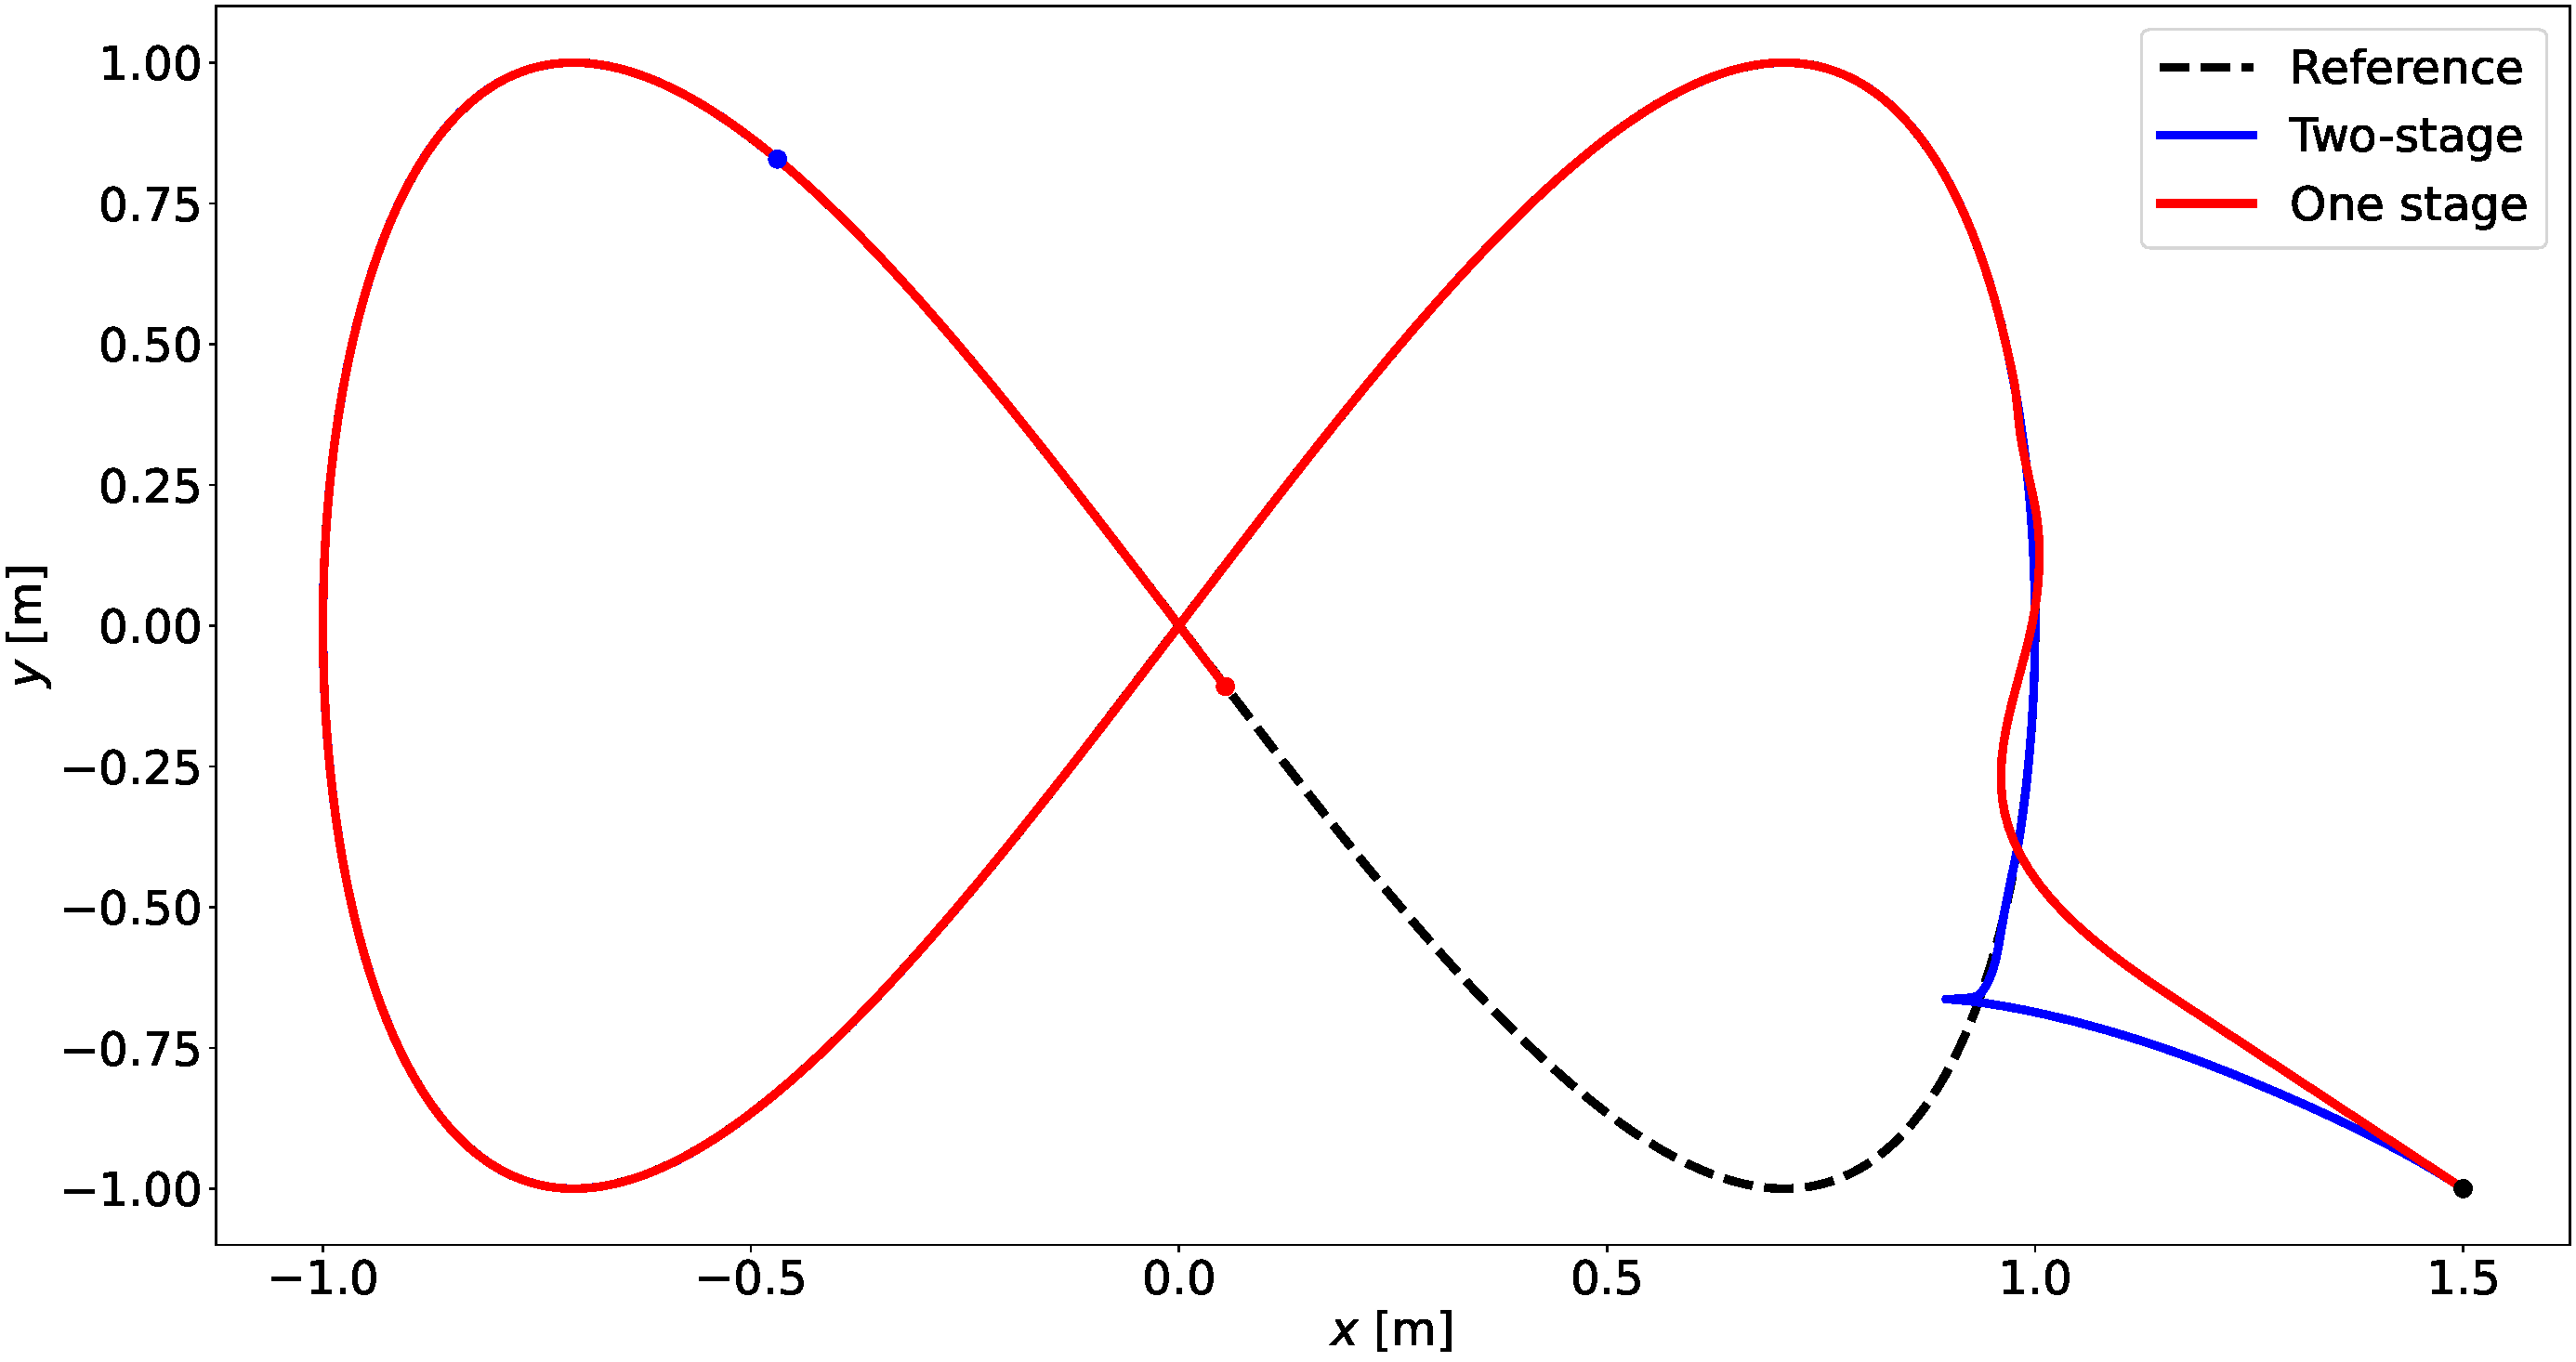
\includegraphics[width=0.49\linewidth]{Figures/one_vs_two_stage_vspeed.pdf}}
%    \subfigure[Constant virtual speed of $0.5$.]{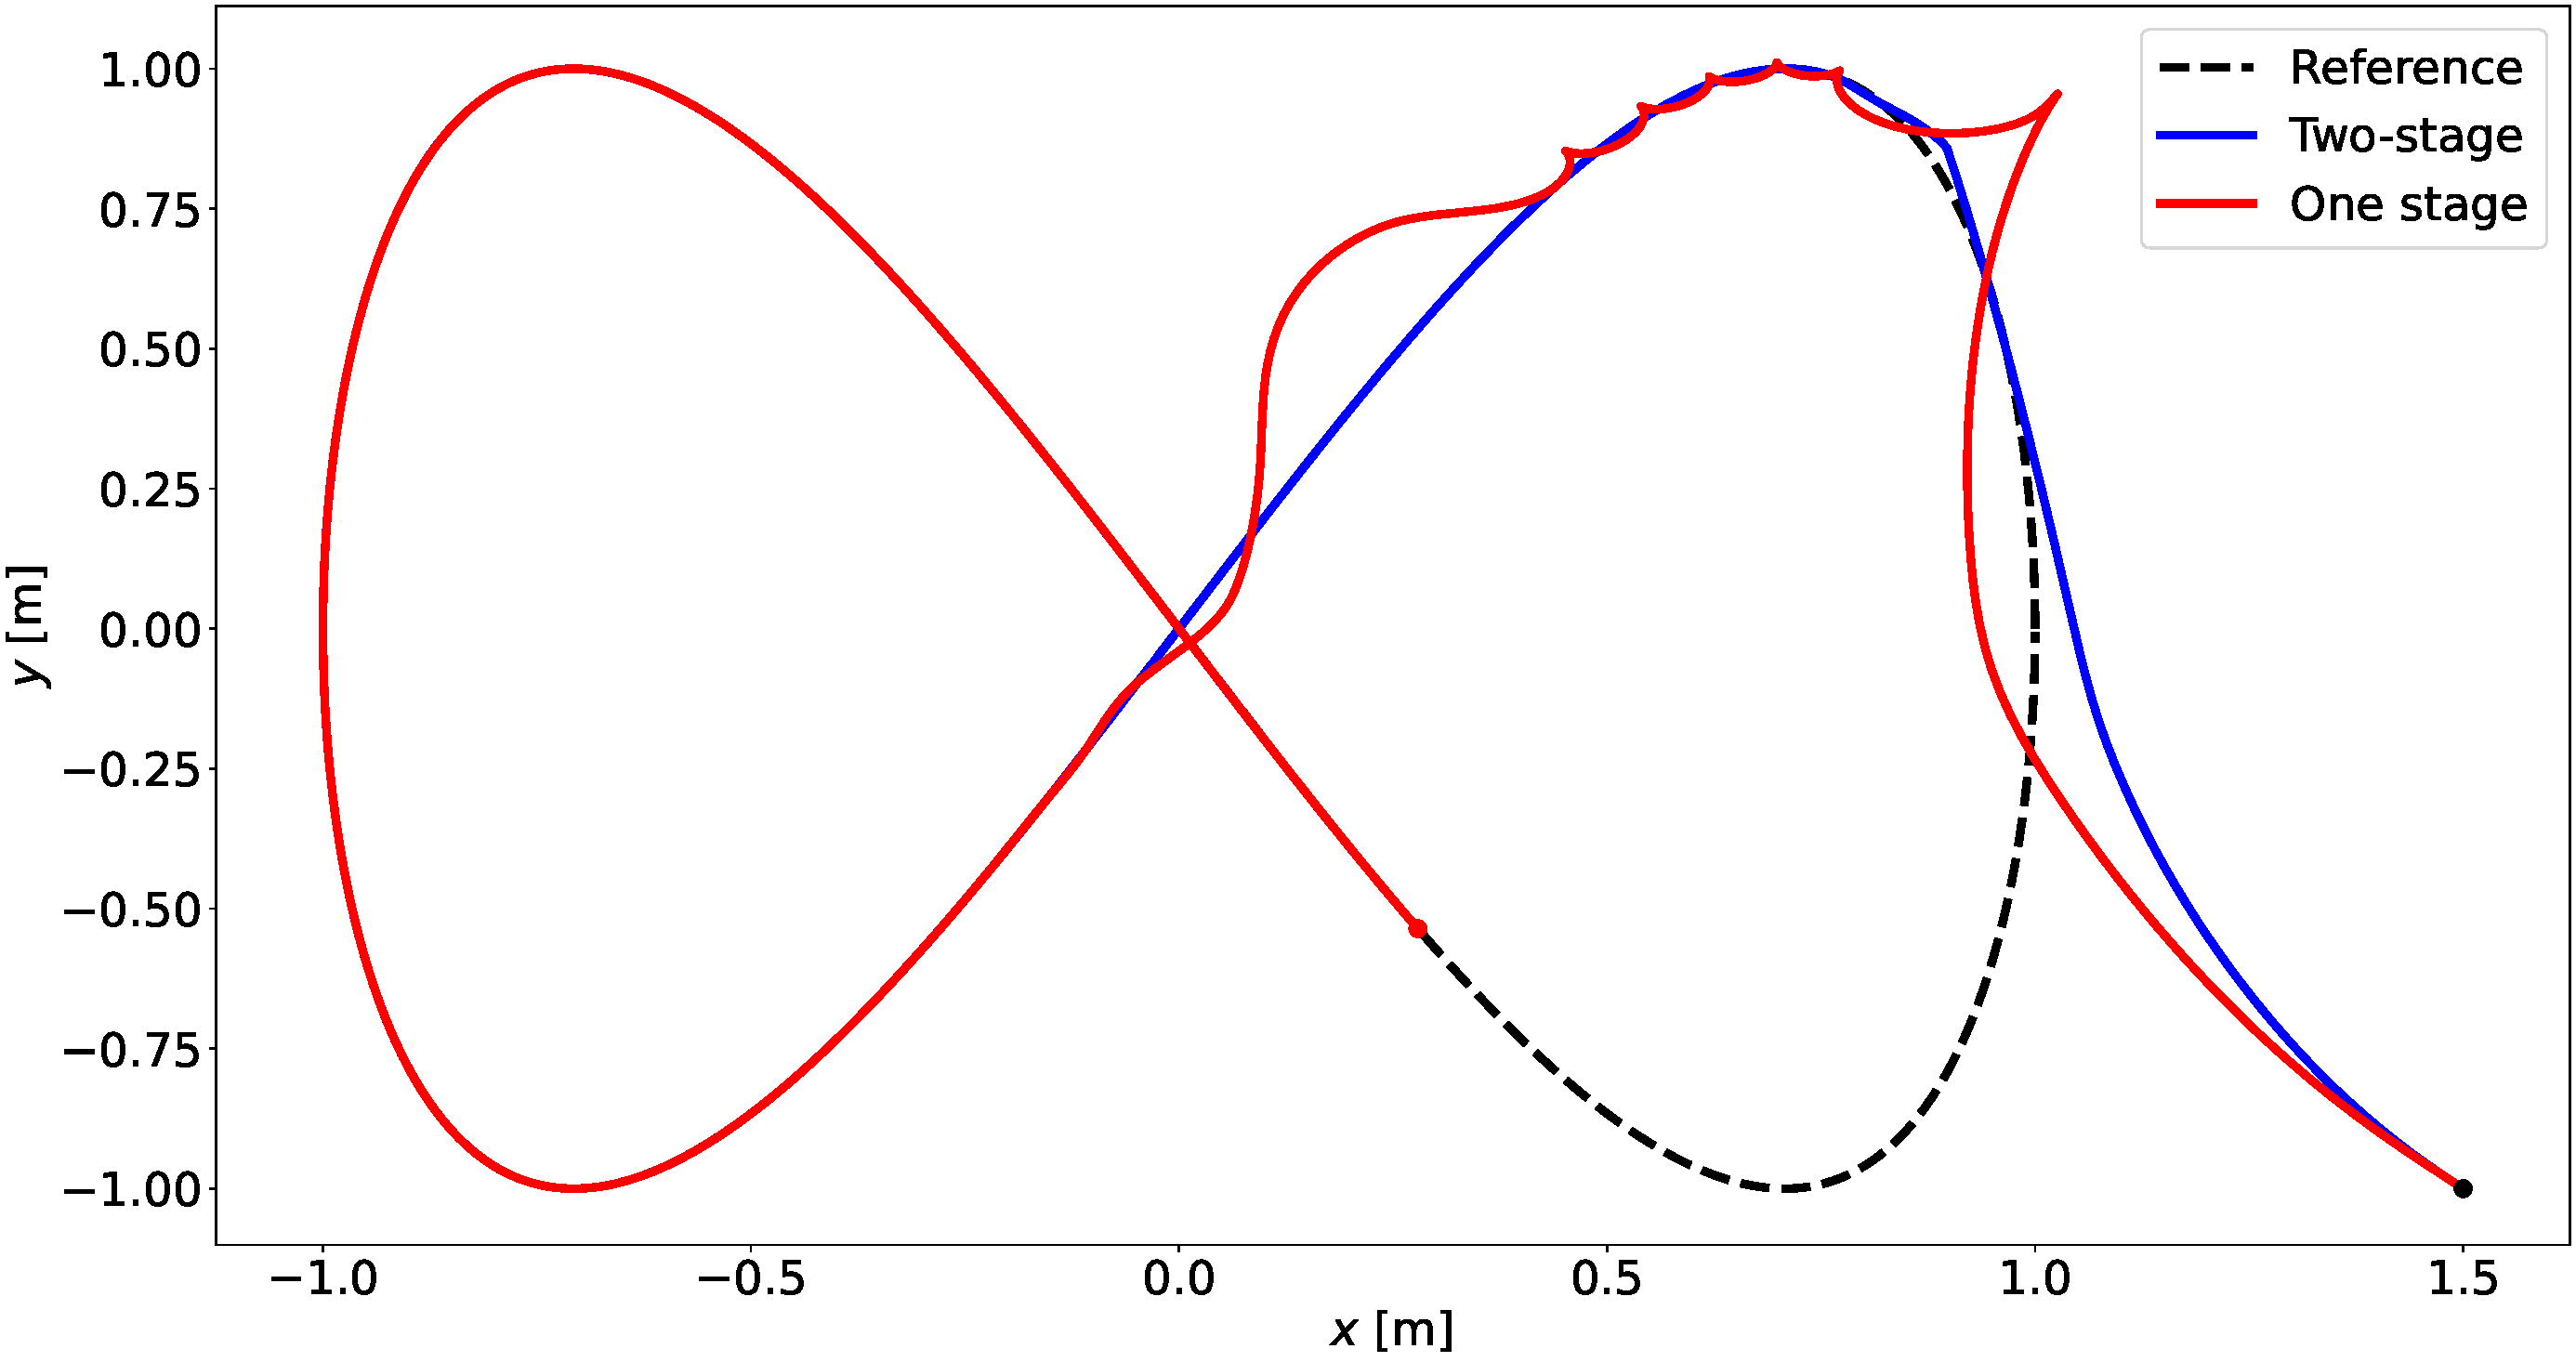
\includegraphics[width=0.49\linewidth]{Figures/one_vs_two_stage_no_vspeed.pdf}}
%  \end{subfigmatrix}
%  \caption{One-stage \textit{vs} two-stage reference tracking.}
%  \label{fig:architecturecomp}
%\end{figure}
%
%\begin{table}[!htb]
%  \caption{Computational cost comparison between different architectures.}
%  \label{tab:compCostarchitecture}
%  \centering
%  \renewcommand{\arraystretch}{1.2}
%  \begin{tabular}{@{}rrrcrr@{}}
%    \toprule
%      & \multicolumn{2}{c}{W/ virtual speed control} & \phantom{abc} & \multicolumn{2}{c}{Constant virtual speed of $0.5$} \\
%    \cmidrule{2-3}
%    \cmidrule{5-6}
%      & Two-stage & One-stage && Two-stage & One-stage \\
%    \midrule
%      Opt. time [ms] & $55.93 \pm 21.95$ & $33.08 \pm 21.59$ && $54.12 \pm 16.12$ & $34.71 \pm 13.20$ \\
%      Cost & $0.27 \pm 1.83$ & $0.36 \pm 2.51$ && $2.24 \pm 10.88$ & $3.56 \pm 16.44$\\
%    \bottomrule
%    \multicolumn{5}{c}{(mean) $\pm$ (standard deviation)}
%  \end{tabular}
%\end{table}
%Both approaches present ups and downs. The two-stage approach main advantage is to break the control algorithm into smaller \acrshort{ocp}s in case too much information is condensed into a single \acrshort{ocp}. On the other hand, the one-stage approach outputs optimal controls much faster. 
%
%In this thesis, one of the main goals is to provide suitable real-time control algorithms, so the optimization time is of utmost importance, so the one-stage approach will be refined and tuned from now on. However, the optimization problem may be reformulated into a two-stage approach in case of need.

%%%%%%%%%%%%%%%%%%%%%%%%%%%%%%%%%%%%%%%%%%%%%%%%%%%%%%%%%%%%%%%%%%%%%%%%
\section{Planar \acrshort{nmpc}}
\label{section:onestageplanarocp}

A general model-based \acrshort{nmpc} is presented in \ref{eq:onestageocp}. In this section, only planar motion is considered ($\roll = \pitch = 0$). The dynamics model is the same as the one in \refeq{eq:skidsteeringStateSpace}. The Lagrange and Mayer terms of the cost function focus on achieving path tracking of the reference but also on keeping the controls rate change not too high, to resemble the fact that on a real system, actuation delays are present.
\begin{subequations}
	\begin{align}
		\begin{split}
			\lagrangeTerm{\mathbf{\x}_k,\,\mathbf{u}_k,\,\mathbf{r},\,\Progress_k,\,\vspeed_k} &= \Vert\left(\x_k - r_{\x}(\Progress_k),\,\y_k - r_{y}(\Progress_k),\,e_{\yaw}\right)\Vert_Q^2 \; +\\ &\Vert\left(\vspeed_k - \vspeed_{ref,\,k},\, \vspeed_k - \vspeed_{k-1},\,\Traction_{l,\,k} - \Traction_{l,\,k-1},\,\Traction_{r,\,k} - \Traction_{r,\,k-1}\right)\Vert_R^2 \label{subeq:onestagelagrange} \\
		\end{split}\\
		\mayerTerm{\mathbf{\x}_k,\,\mathbf{r},\,\Progress_k} &= \Vert\left(\x_k - r_{\x}(\Progress_k),\,\y_k - r_{\y}(\Progress_k),\,e_{\yaw}\right)\Vert_Q^2 \label{subeq:onestagemayer} \\
		e_{\yaw} &= \left(\cos\left(\yaw_k\right) - \cos\left(r_{\yaw}(\Progress_k)\right)\right)^2 + \left(\sin\left(\yaw_k\right) - \sin\left(r_{\yaw}(\Progress_k)\right)\right)^2 \label{subeq:rotationInvtrick}
	\end{align}
\end{subequations}

Equation \eqref{subeq:rotationInvtrick} denotes the rotational invariance trick \cite{schoels2020nmpc}, that aims to prevent ambiguities and unnecessary rotations when $\yaw_k - \yaw_{ref}\left(\Progress_k\right) \geq 2 \pi$. The cost \eqref{subeq:costonestage} also aims to keep the virtual speed, $\vspeed$, somewhat constant but also to promote progress along the reference. 
\begin{subequations}
	\begin{align}
		\underset{\mathbf{x}_k,\,\mathbf{u}_k,\,\Progress_k,\,\vspeed_k}{\text{minimize}} &\sum_{k=0}^{N-1} \lagrangeTerm{\mathbf{\x}_k,\,\mathbf{u}_k,\,\mathbf{r},\,\Progress_k,\,\vspeed_k} + \mayerTerm{\mathbf{\x}_N,\,\mathbf{r},\,\Progress_k} \label{subeq:costonestage} \\
		\text{subject to}&
		\begin{cases}
			\mathbf{x}_{0,\,i} =\mathbf{\hat{x}}_{0,\,i-1}\\
			\Progress_{0,\,i} = \Progress^*_{1,\,i-1}\\
			\DerMathBold{x}(t) = \processModel{\mathbf{x}(t), \mathbf{u}(t), \mathbf{p}} \quad\text{(equation \ref{eq:skidsteeringStateSpace})}\\
			\dot{\Progress} = \vspeed\\
			\ineqCon{\mathbf{x}_k,\,\mathbf{u}_k,\,\mathbf{p}} \leq 0 \quad \text{(equation \ref{eq:skidsteeringcoulomb})}\\
			\vspeed_{min} \leq \vspeed \leq \vspeed_{max}
		\end{cases}
	\end{align}
	\label{eq:onestageocp}
\end{subequations}

Apart from the dynamics model that is presented in continuous time, the cost function and inequality constraints are presented in discrete time. \acrshort{nmpc} \eqref{eq:onestageocp} is presented this way to closely match the implementation within the Opti-stack. The Opti-stack takes care of the dynamics discretization.

In case the virtual speed is controlled within the \acrshort{nmpc}, the reference is also defined in the solver, which depends on the progress variable $\Progress_k$. Moreover, $\Progress$ is also a state and $\vspeed$ a control. In case the reference path is provided to the solver, that dependence vanishes, and $\Progress$ and $\vspeed$ are removed from \acrshort{nmpc} \eqref{eq:onestageocp}. The virtual speed is an unitless variable and not necessarily a parameterized velocity. Its goal is to speed up or delay the traversal of some reference. Finally, the parameters $\mathbf{p}$ are kept constant throughout the control horizon.

\subsection{Planar \acrshort{nmpc} architectures}
\label{subsection:onestageocparch}

When it comes to the inclusion of the virtual speed control into the optimization model, this choice depends on the kind of reference the mobile robot follows up. The solver may be fed with points from a path that the robot needs to catch up with, where the reference virtual speed is controlled outside the solver by changing the gap between consecutive points. Conversely, the virtual speed may be controlled inside the \acrshort{nmpc} if the reference analytical equations are provided to the solver. The latter may add non-negligible overhead to the solver, but the virtual speed control may be removed in case real-time requirements are not met.

Figure \ref{fig:onestagearchitecturecomp} presents the architecture of both variations. Each \acrshort{nmpc} is always fed with the optimal solution of the previous iteration. Then, every optimal solution is shifted and the optimization problem initial guess is filled as it is described in \refeq{eq:shifting}.

\begin{figure}[!htb]
    \subfigure[Virtual speed control inside \acrshort{nmpc}] {
	    \tikzstyle{block} = [draw, text centered, minimum height = 2.0em,minimum width = 3.0em, rounded corners, line width = 0.5 mm]
	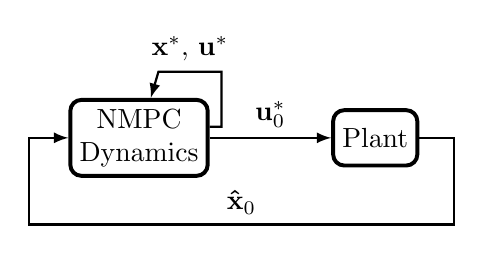
\begin{tikzpicture}
		\node [block, align= center] at (0, 0) (2) {NMPC\\Dynamics};
		\node [block, align= center] at (3.0, 0) (3) {Plant};
  		\draw [-latex,thick, align = center] (2) -- node [above] {$\mathbf{u}_0^*$} (3);
  		\draw [-latex, thick, align = center] (3)
    											-- ++(1.0, 0.0)
    											-- ++(0.0, -1.1)
    											-- node[above]{$\mathbf{\hat{x}}_0$} ++(-5.4, 0.0)
    											-- ++(0.0, 1.1)
    											-- (2);
		\draw [-latex, thick, align=center] ([yshift=4.0]2.east)
		-- ++(0.15, 0.0)
		-- ++(0.0, 0.7)
		-- node[above] {$\mathbf{x}^*,\,\mathbf{u}^*$} ++(-0.8, 0.0)
		-- (2);
	\end{tikzpicture}
	\label{subfig:archvspeedinsideocp}
    }
    \subfigure[Virtual speed control outside \acrshort{nmpc}]{
		\tikzstyle{block} = [draw, text centered, minimum height = 2.0em, minimum width = 3.0em, rounded corners, line width = 0.5 mm]
	\begin{tikzpicture}
		\node [block, align= center, draw={rgb,255:red,30;green,145;blue,30}] at (0.8, 0) (2) {\textcolor{rgb,255:red,30;green,145;blue,30}{Virtual speed control}};
		\node [block, align = center] at (4.0, 0) (3) {NMPC\\Dynamics};
		\node [block, align = center] at (7.0, 0) (4) {Plant};
  		\draw [-latex, thick, align = center] (4)
  												 -- ++(1.0, 0.0)
  												 -- ++(0.0, -1.1)
  												 -- coordinate (bottomSeg) node [above, xshift=-2em] {$\mathbf{\hat{x}}_0$} ++(-9.4, 0.0)
  												 -- ++(0.0, 1.1)
  												 -- (2);
  												 
    	\coordinate (pointBelow3) at ($(3 |- bottomSeg)$);
    	\filldraw[black] (pointBelow3) circle (1pt);
  		\draw [-latex, thick, align=center] ([yshift=4.0]3.east)
		-- ++(0.15, 0.0)
		-- ++(0.0, 0.7)
		-- node[above] {$\mathbf{x}^*,\,\mathbf{u}^*$} ++(-0.8, 0.0)
		-- (3);
  		\draw [-latex,thick] (2) -- node [above] {$\mathbf{r}$} (3);
  		\draw [-latex,thick] (3) -- node [above] {$\mathbf{u}_0^*$} (4);
  		\draw [-latex, thick] (pointBelow3) -- (3);
	\end{tikzpicture}
	\label{subfig:archvspeedoutsideocp}
    }
  \caption{Planar \acrshort{nmpc} architectures}
  \label{fig:onestagearchitecturecomp}
\end{figure}

\subsubsection*{Closest path point to initial position}

At the start of the simulation, it is important to feed the controller with the closest path point to the robot. This prevents the mobile robot from traversing an unnecessary distance (and possibly unsafe) to meet the path where $\Progress = 0$. Then, the mobile robot can start tracking the path at its closest point. This resembles the fact that, on uneven terrain, it is safer for the mobile robot to traverse previously surveyed terrain, and not go through unknown areas.
\begin{eqnarray}
  {\rm Minimize}   && \left(\x_0 - r_{\x}(\Progress)  \right)^2 + \left(\y_0 - r_{\y}(\Progress)\right)^2 \label{eq:closestPoint}\\
  {\rm w.r.t.}     && {\Progress} \nonumber
\end{eqnarray}

\acrshort{nlp} \eqref{eq:closestPoint} is implemented in Opti and \acrshort{ipopt} is the solver. Its solution $\Progress^*$ is used to define the initial path point that the controller will be aiming to track. The initial guess is determined by dividing the reference on equal spaces and retrieving the progress of the closest point.

\begin{figure}[!htb]
	\centering
	\subfigure[Advantage of closest point optimization.]{
        \centering
        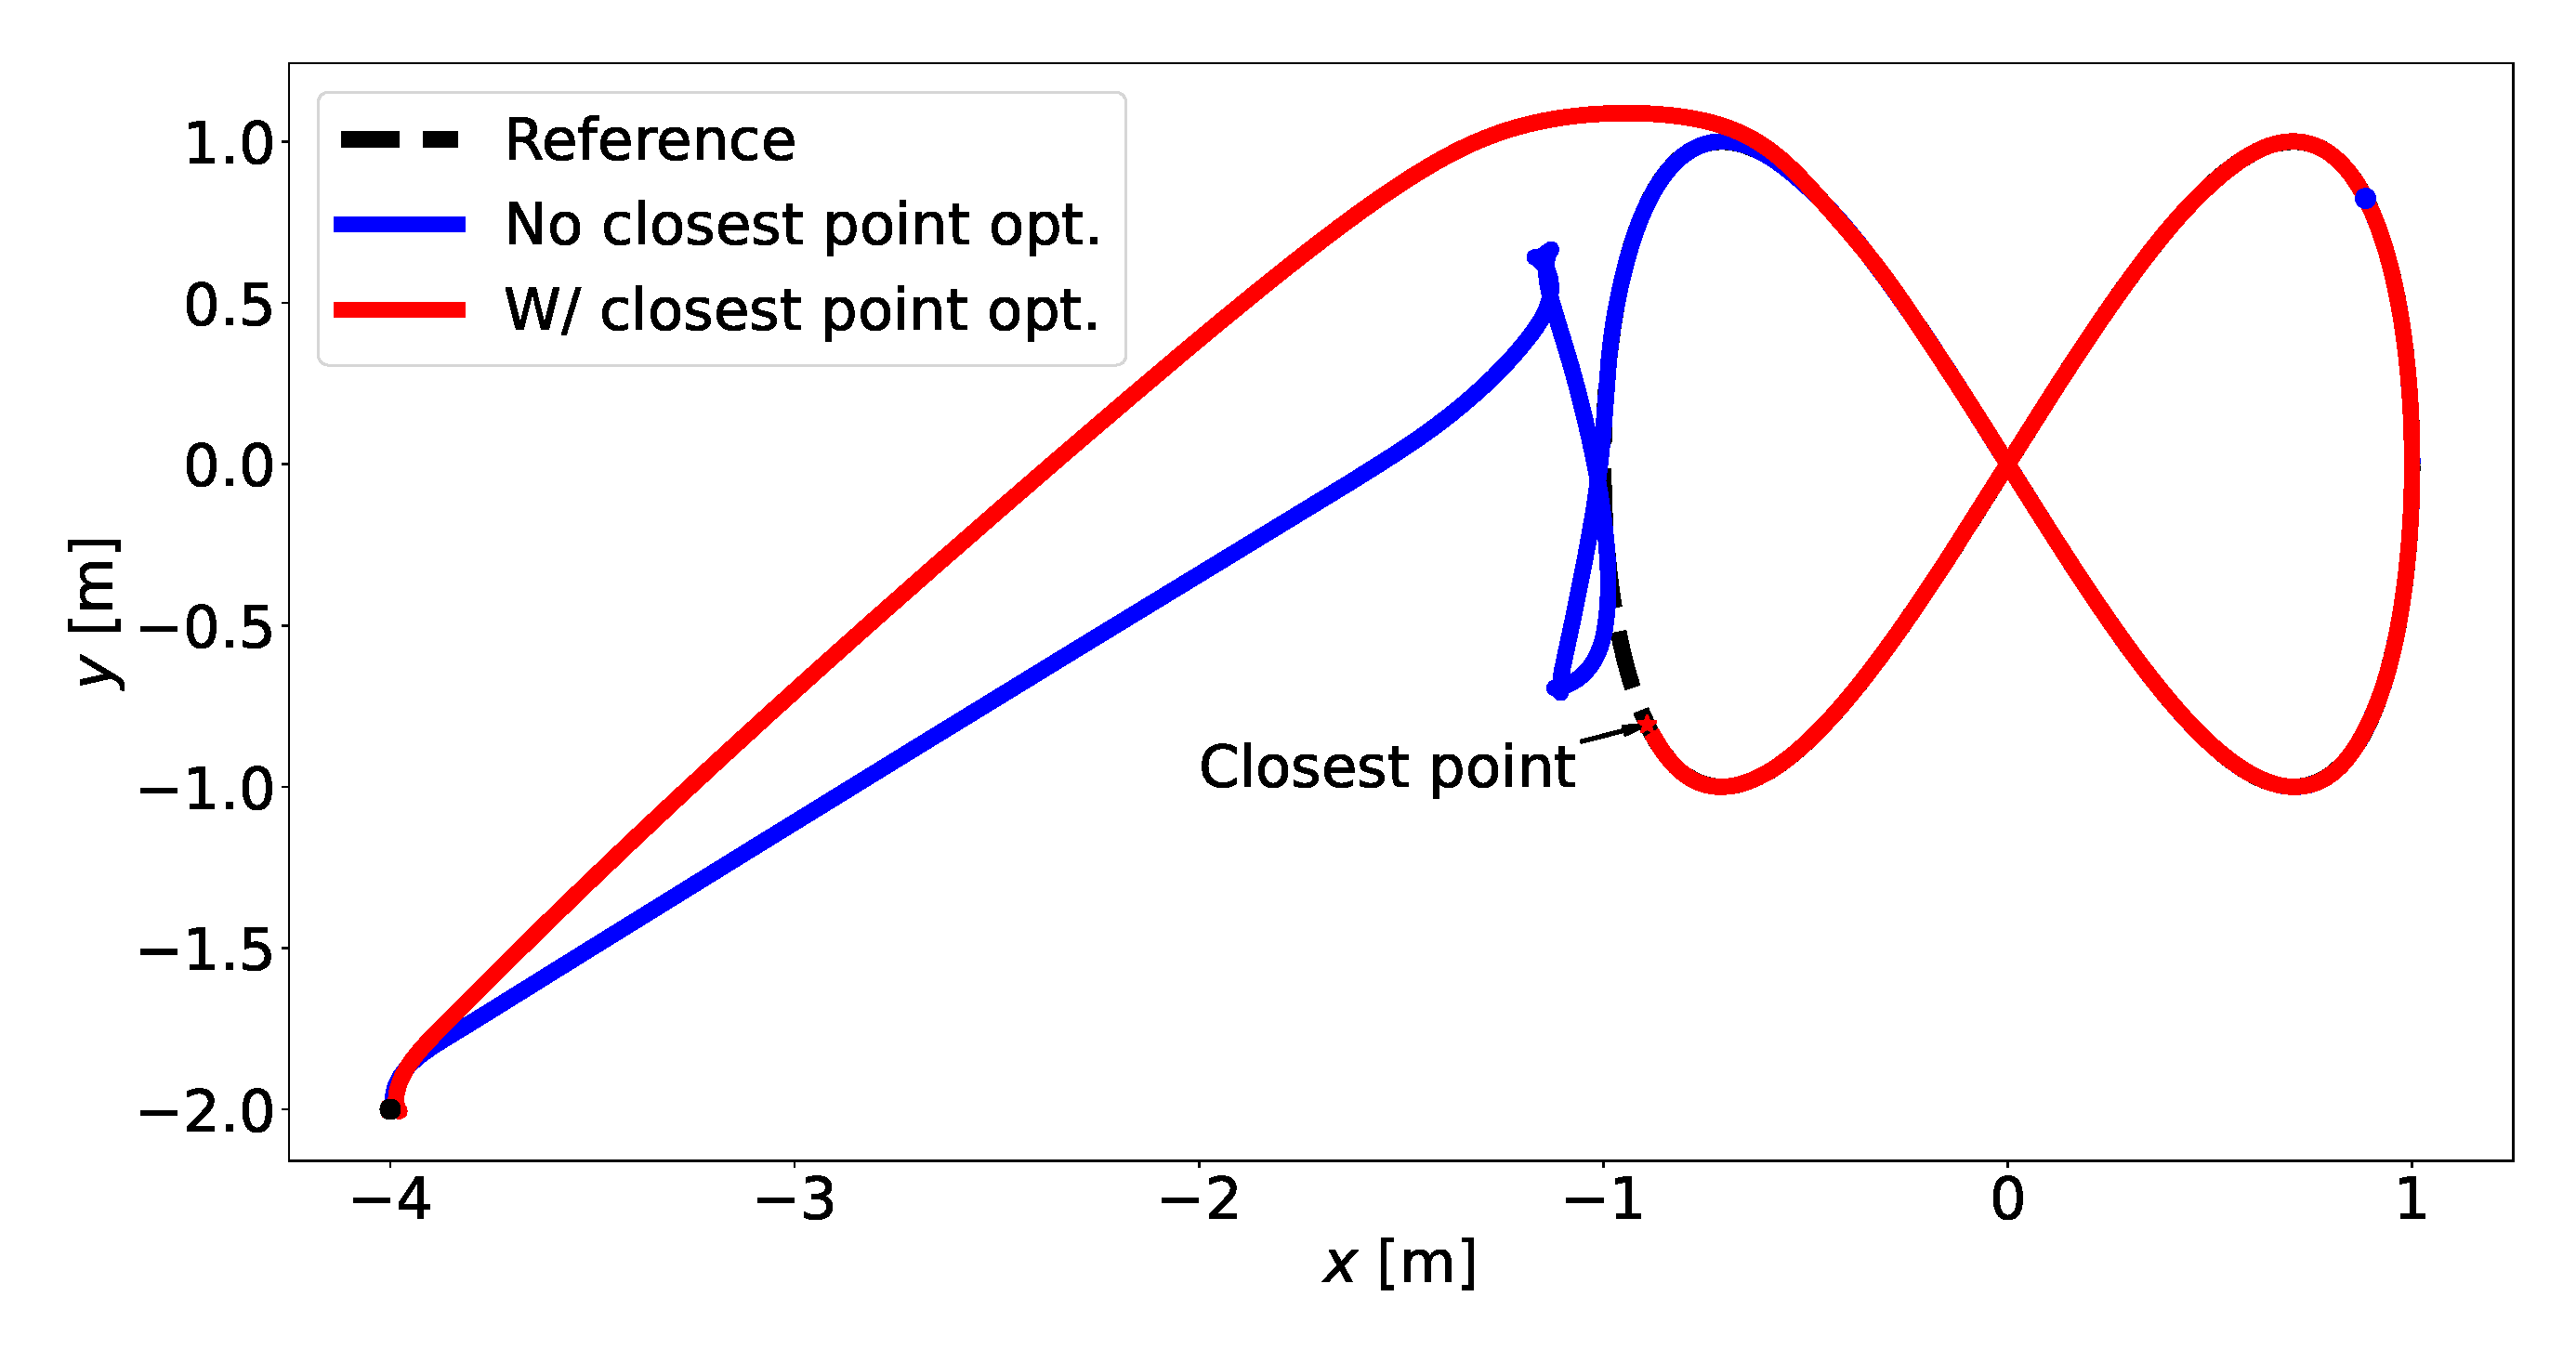
\includegraphics[width=0.495\textwidth]{Figures/One stage OCP/Closest point analysis/closest_point_comp.pdf}
        \label{fig:closestPoint_comp}
	}
	\hspace{-1.9em}
    \subfigure[Path tracking from different initial positions.]{
        \centering
        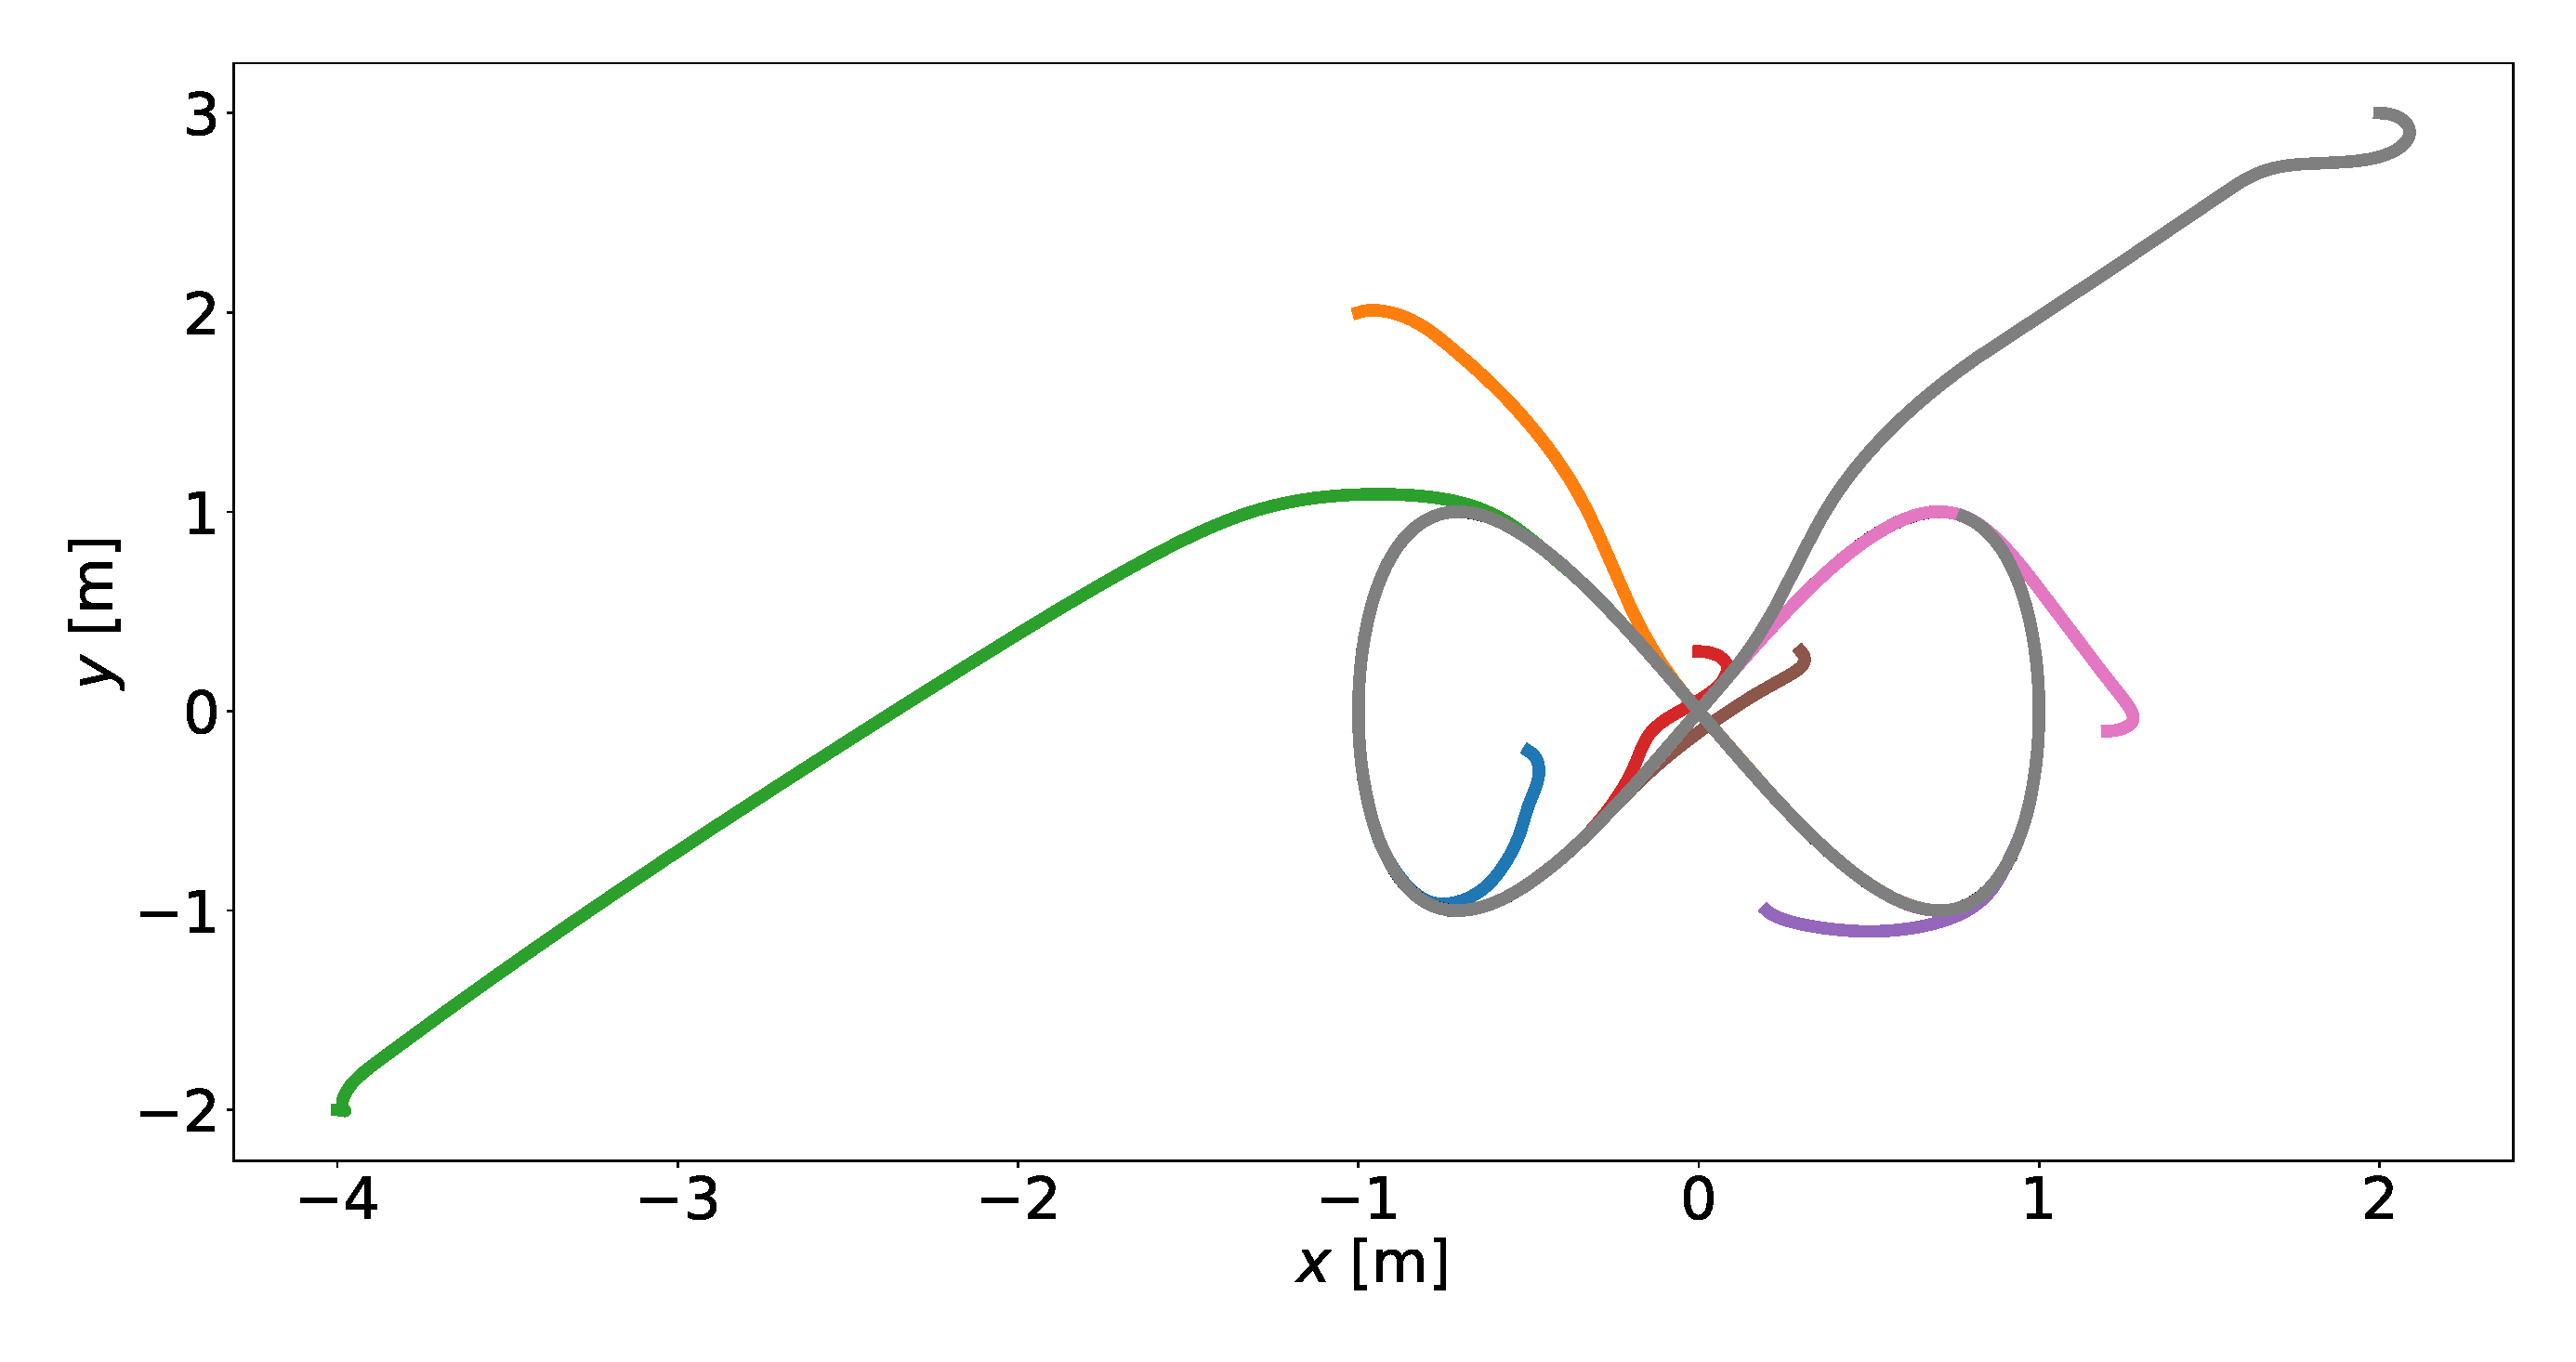
\includegraphics[width=0.495\textwidth]{Figures/One stage OCP/Closest point analysis/closest_point_comp_initialpoints.pdf}
        \label{fig:closestPoint_comp_initial_points}
	}
	\caption{Path tracking improvements due to solver initialization with closest point progress.}
	\label{fig:PathTrackImprovementsClosestPoint}
\end{figure}

Figure \ref{fig:closestPoint_comp} presents a comparison of the path traversed by a mobile robot in case the very first point tracked is the one where $\Progress = 0$, or in case $\Progress$ points to the closest point of the trajectory at the initial position of the mobile robot. When the initial state of $\Progress$ points to the closest point, the path traversed by the mobile robot is much smoother. When the closest point is unknown to the controller, the controller (\ref{eq:onestageocp}) tries to move the reference closer to the mobile robot from far away, which causes the mobile robot to perform very sharp turns before \textit{catching} the reference. In figure \ref{fig:closestPoint_comp_initial_points}, it is observed that all paths are smooth regardless of the initial pose. The simulations presented in figure \ref{fig:PathTrackImprovementsClosestPoint} were performed with virtual speed control within the controller.

\subsection{Solver parameters survey}
\label{subsection:solverspecssurvey}

After the baseline \acrshort{nmpc} architectures are set, it is time to refine the \acrshort{nmpc} by playing with the control horizon, sampling time and weights of the cost function.

Firstly, the problem is reformulated by adding a term on the cost function that aims to account for the control effort, so that the battery of the vehicle is saved as much as possible. Then, \refeq{subeq:onestagelagrange} becomes,
\begin{equation}
	\begin{split}
		\lagrangeTerm{\mathbf{\x}_k,\,\mathbf{u}_k,\,\mathbf{r},\,\Progress_k,\,\vspeed_k} &= \Vert\left(\x_k - r_{\x}(\Progress_k),\,\y_k - r_{\y}(\Progress_k),\,e_{\yaw}\right)\Vert_Q^2 \; +\\&\Vert\left(\vspeed_k - \vspeed_{ref,\,k},\, \vspeed_k - \vspeed_{k-1},\,\Traction_{l,\,k} - \Traction_{l,\,k-1},\,\Traction_{r,\,k} - \Traction_{r,\,k-1},\,\Traction_{l,\,k},\,\Traction_{r,\,k}\right)\Vert_R^2
	\end{split}
	\label{eq:reflagrange}
\end{equation}

The rest of the solver's structure remains unchanged. Both controllers architectures are evaluated separately. Some performance metrics are selected, that take into account the cumulatives control effort, position and heading errors, as well as the progress made by the vehicle. The cumulative position and heading errors are given by $\varepsilon_i = \sum_i \sqrt{ (\x_i - r_{\x,\,i})^2 + (\y_i - r_{\y,\,i})^2 }$ and $\sum_i e_{\yaw,\,i}$, respectively. The cumulative control effort is designed to get an idea of the electric energy spent by the vehicle, that is $\sum_i \left(\Traction_{l,\,i} + \Traction_{r,\,i}\right)\,T_{c,\,i}$.

In case the virtual speed is controlled inside the \acrshort{nmpc}, $\vspeed_{ref,\,k} = 0.5,\;\forall\,k$. For the opposite case, the reference path is generated by determining a virtual speed, which is generated as follows,

\begin{equation}
v_i\left(\kappa,\,\varepsilon\right) = min\left( \frac{0.5}{ 1 + \exp\left( 5.0\times( \varepsilon - 2.0 ) \right) },\, \frac{0.5}{ 1 + \exp\left( 0.1 \times ( \kappa - 10.0 ) \right) } \right)
\label{eq:vspeed_computation_architecture_b}
\end{equation}

\noindent, where $\varepsilon$ and $\kappa$ denote the positional error and curvature at the current progress, respectively.

The results presented below were generated on an Intel® Core™ i7-10750H CPU @ 2.60GHz × 12 processor. The \acrshort{nmpc}s were formulated in the Opti stack and \acrshort{ipopt} was used as solver. Real-time specs were neglected at this point.

\subsubsection*{Control horizon}

The simulation results of the planar \acrshort{nmpc} with respect to the control horizon are presented in figure \ref{fig:PathTrackCompHorizonVar} and tables \ref{tab:cumulativeControlEffortControlHorizon}, \ref{tab:cumulativePositionalErrorControlHorizon} and \ref{tab:cumulativeHeadingErrorControlHorizon}. The parameters of the solver that are kept constant on every simulation are stated in table \ref{tab:controlHorizonSpecs}. The order of $Q$ and $R$ diagonal elements is aligned with the order of the cost terms presented in equations \eqref{eq:reflagrange} and \eqref{subeq:onestagemayer}.

\begin{table}[!htb]
  \caption[Constant solver parameters when control horizon changes.]{Constant solver parameters.}
  \label{tab:controlHorizonSpecs}
  \renewcommand{\arraystretch}{1.2}
  \centering
  \begin{tabular}[]{ccccccc}
	\toprule
        $Q$ & $R$ & $\SamplingTime\,[ms]$\\
	\midrule
        $diag\left(3.0,\,3.0,\,3.0\right)$ & $diag\left(1\mathrm{e}{-3}
,\, 1\mathrm{e}{-6},\,1\mathrm{e}{-6},\,1\mathrm{e}{-6},\,1\mathrm{e}{-9},\,1\mathrm{e}{-9}\right)$ & $10.0$\\
	\toprule
		$\left[(v_x)_{min},\; (v_x)_{max}\right]\,[m/s]$ & $\left[(\omega_z)_{min},\; (\omega_z)_{max}\right]\,[rad/s]$ & $\left[v_{min},\;v_{max}\right]$ & $\FrictionCoefficient$\\
	\midrule
		$[0.0,\;2.0]$ & $[-10.0,\;10.0]$ & $[0.0,\;1.0]$ & $1.0$\\
  	\bottomrule
  \end{tabular}
\end{table}

\begin{figure}[!htb]
	\centering
	\subfigure[Controlled virtual speed inside \acrshort{nmpc}]{
        \centering
        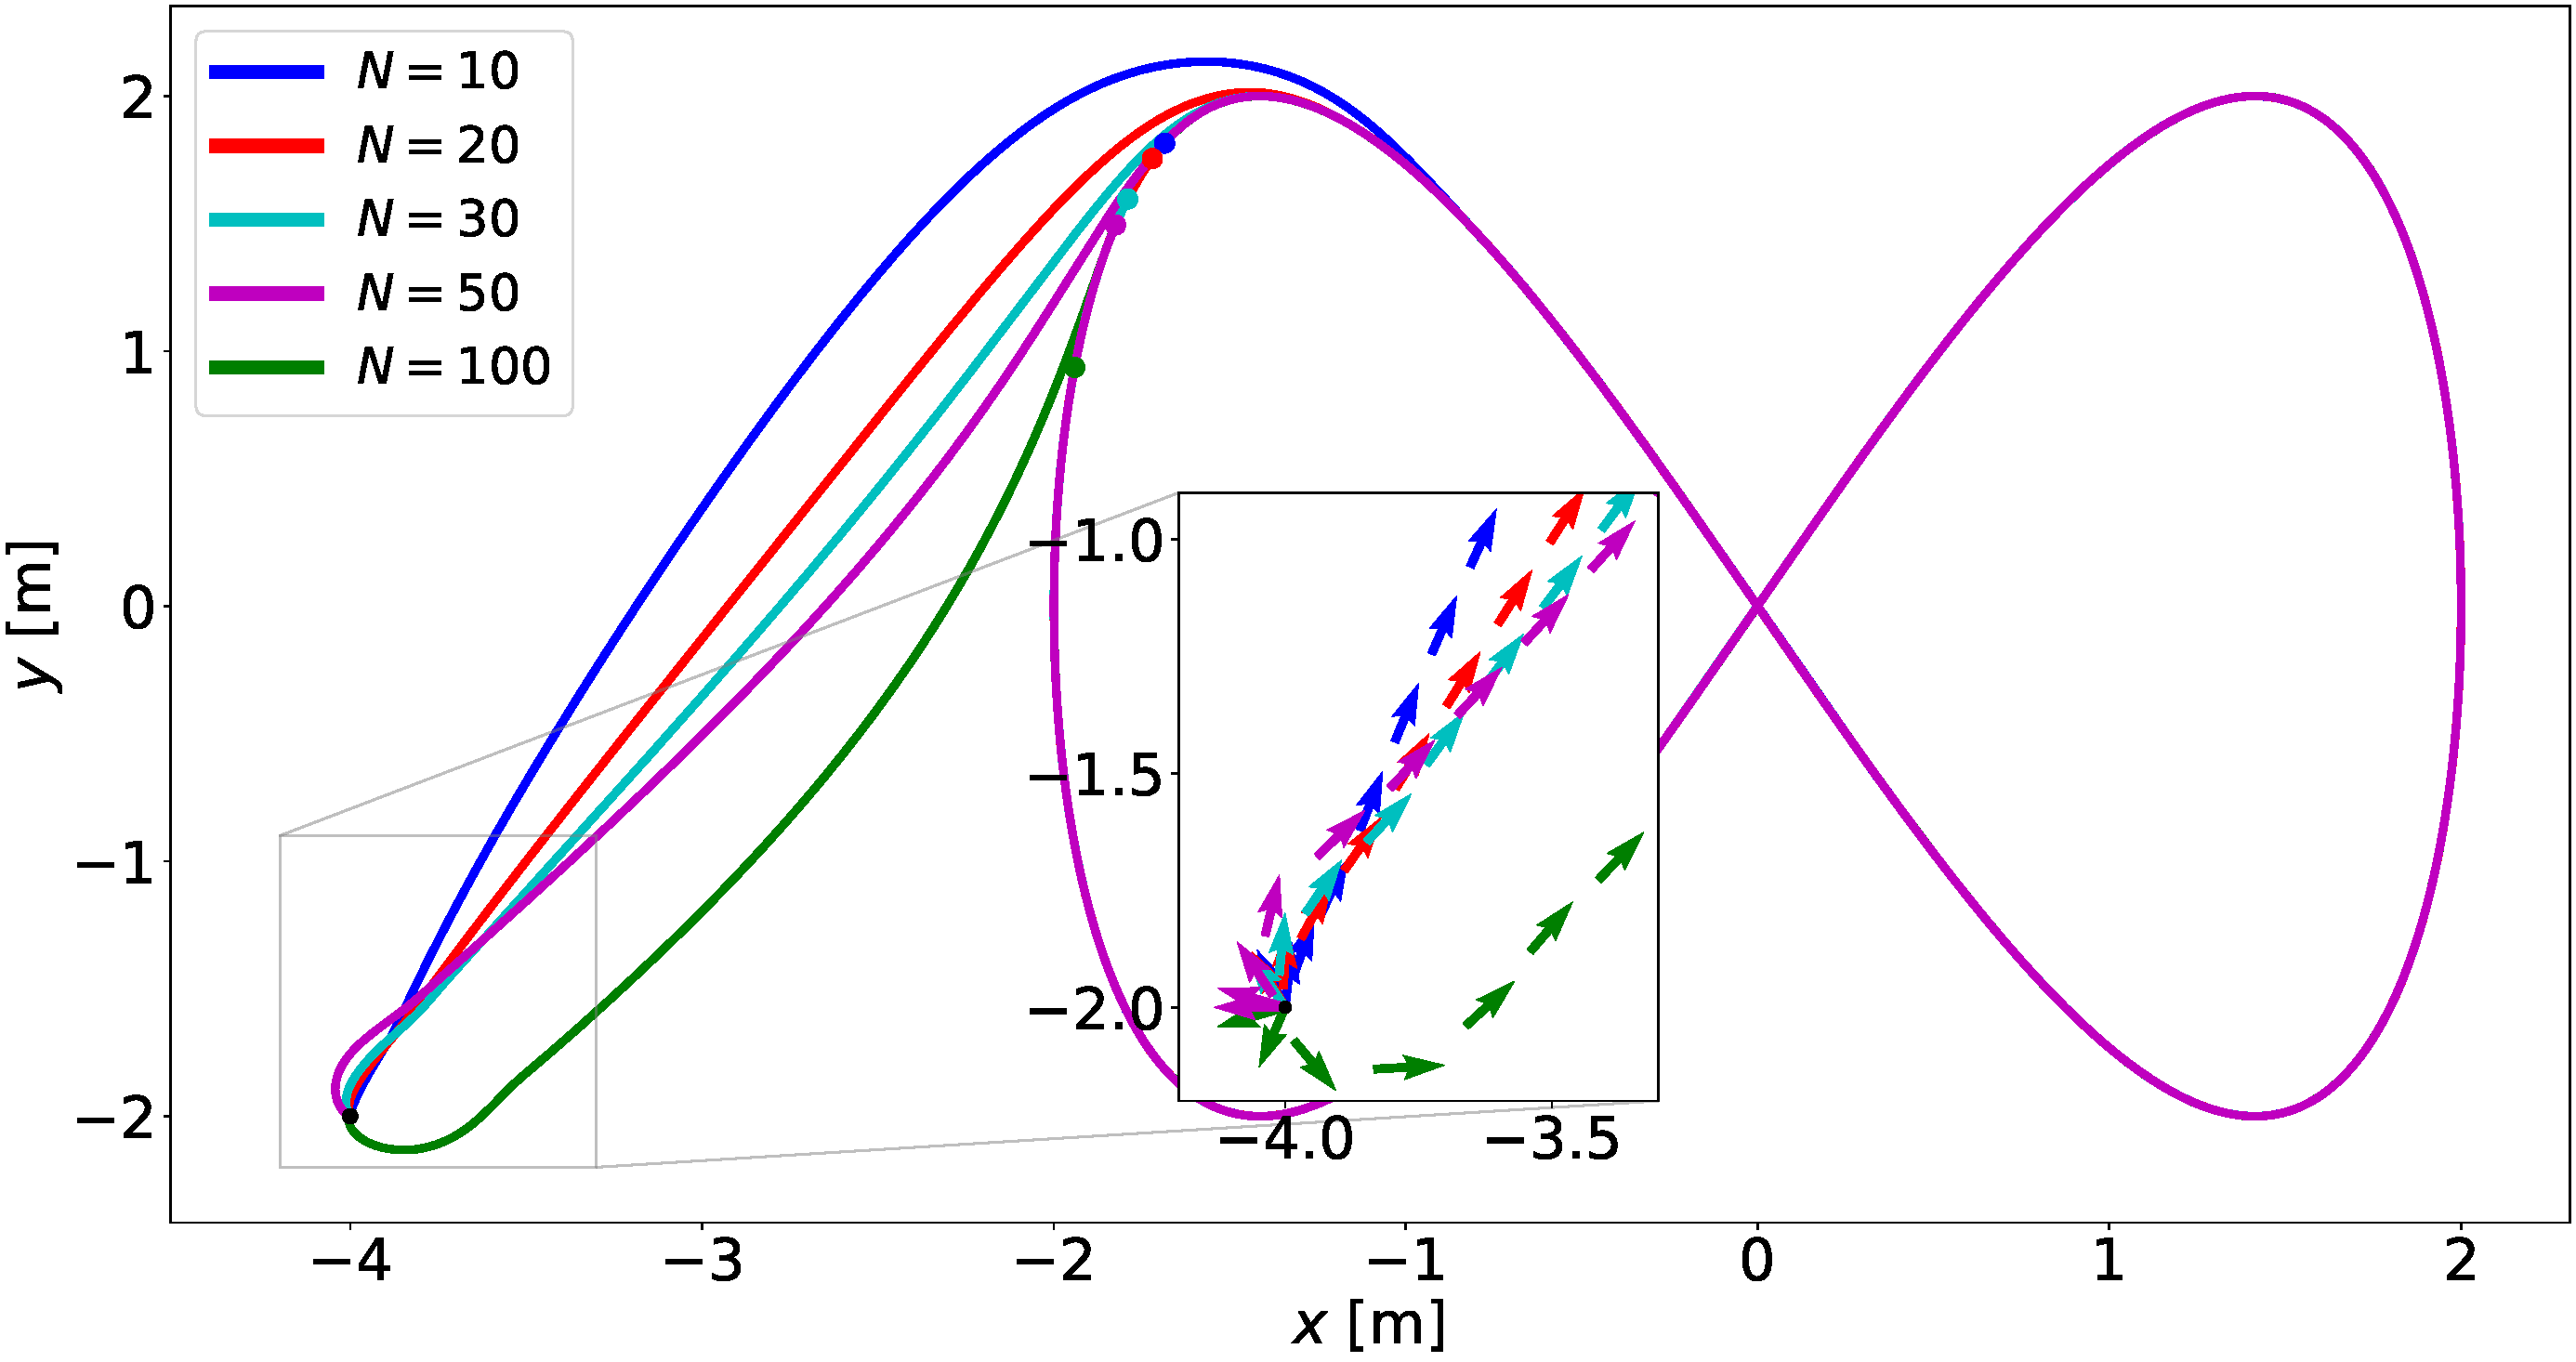
\includegraphics[width=0.48\textwidth]{Figures/One stage OCP/Solver specs comparison/horizon/Virtual speed controlled inside OCP/Planar_onestage_ocp_control_vspeed_comp_horizon.pdf}
        \label{subfig:PathTrackCompHorizonVarInsideVspeed}
	}
	\hspace{-1.0em}
    \subfigure[Controlled virtual speed outside \acrshort{nmpc}]{
        \centering
        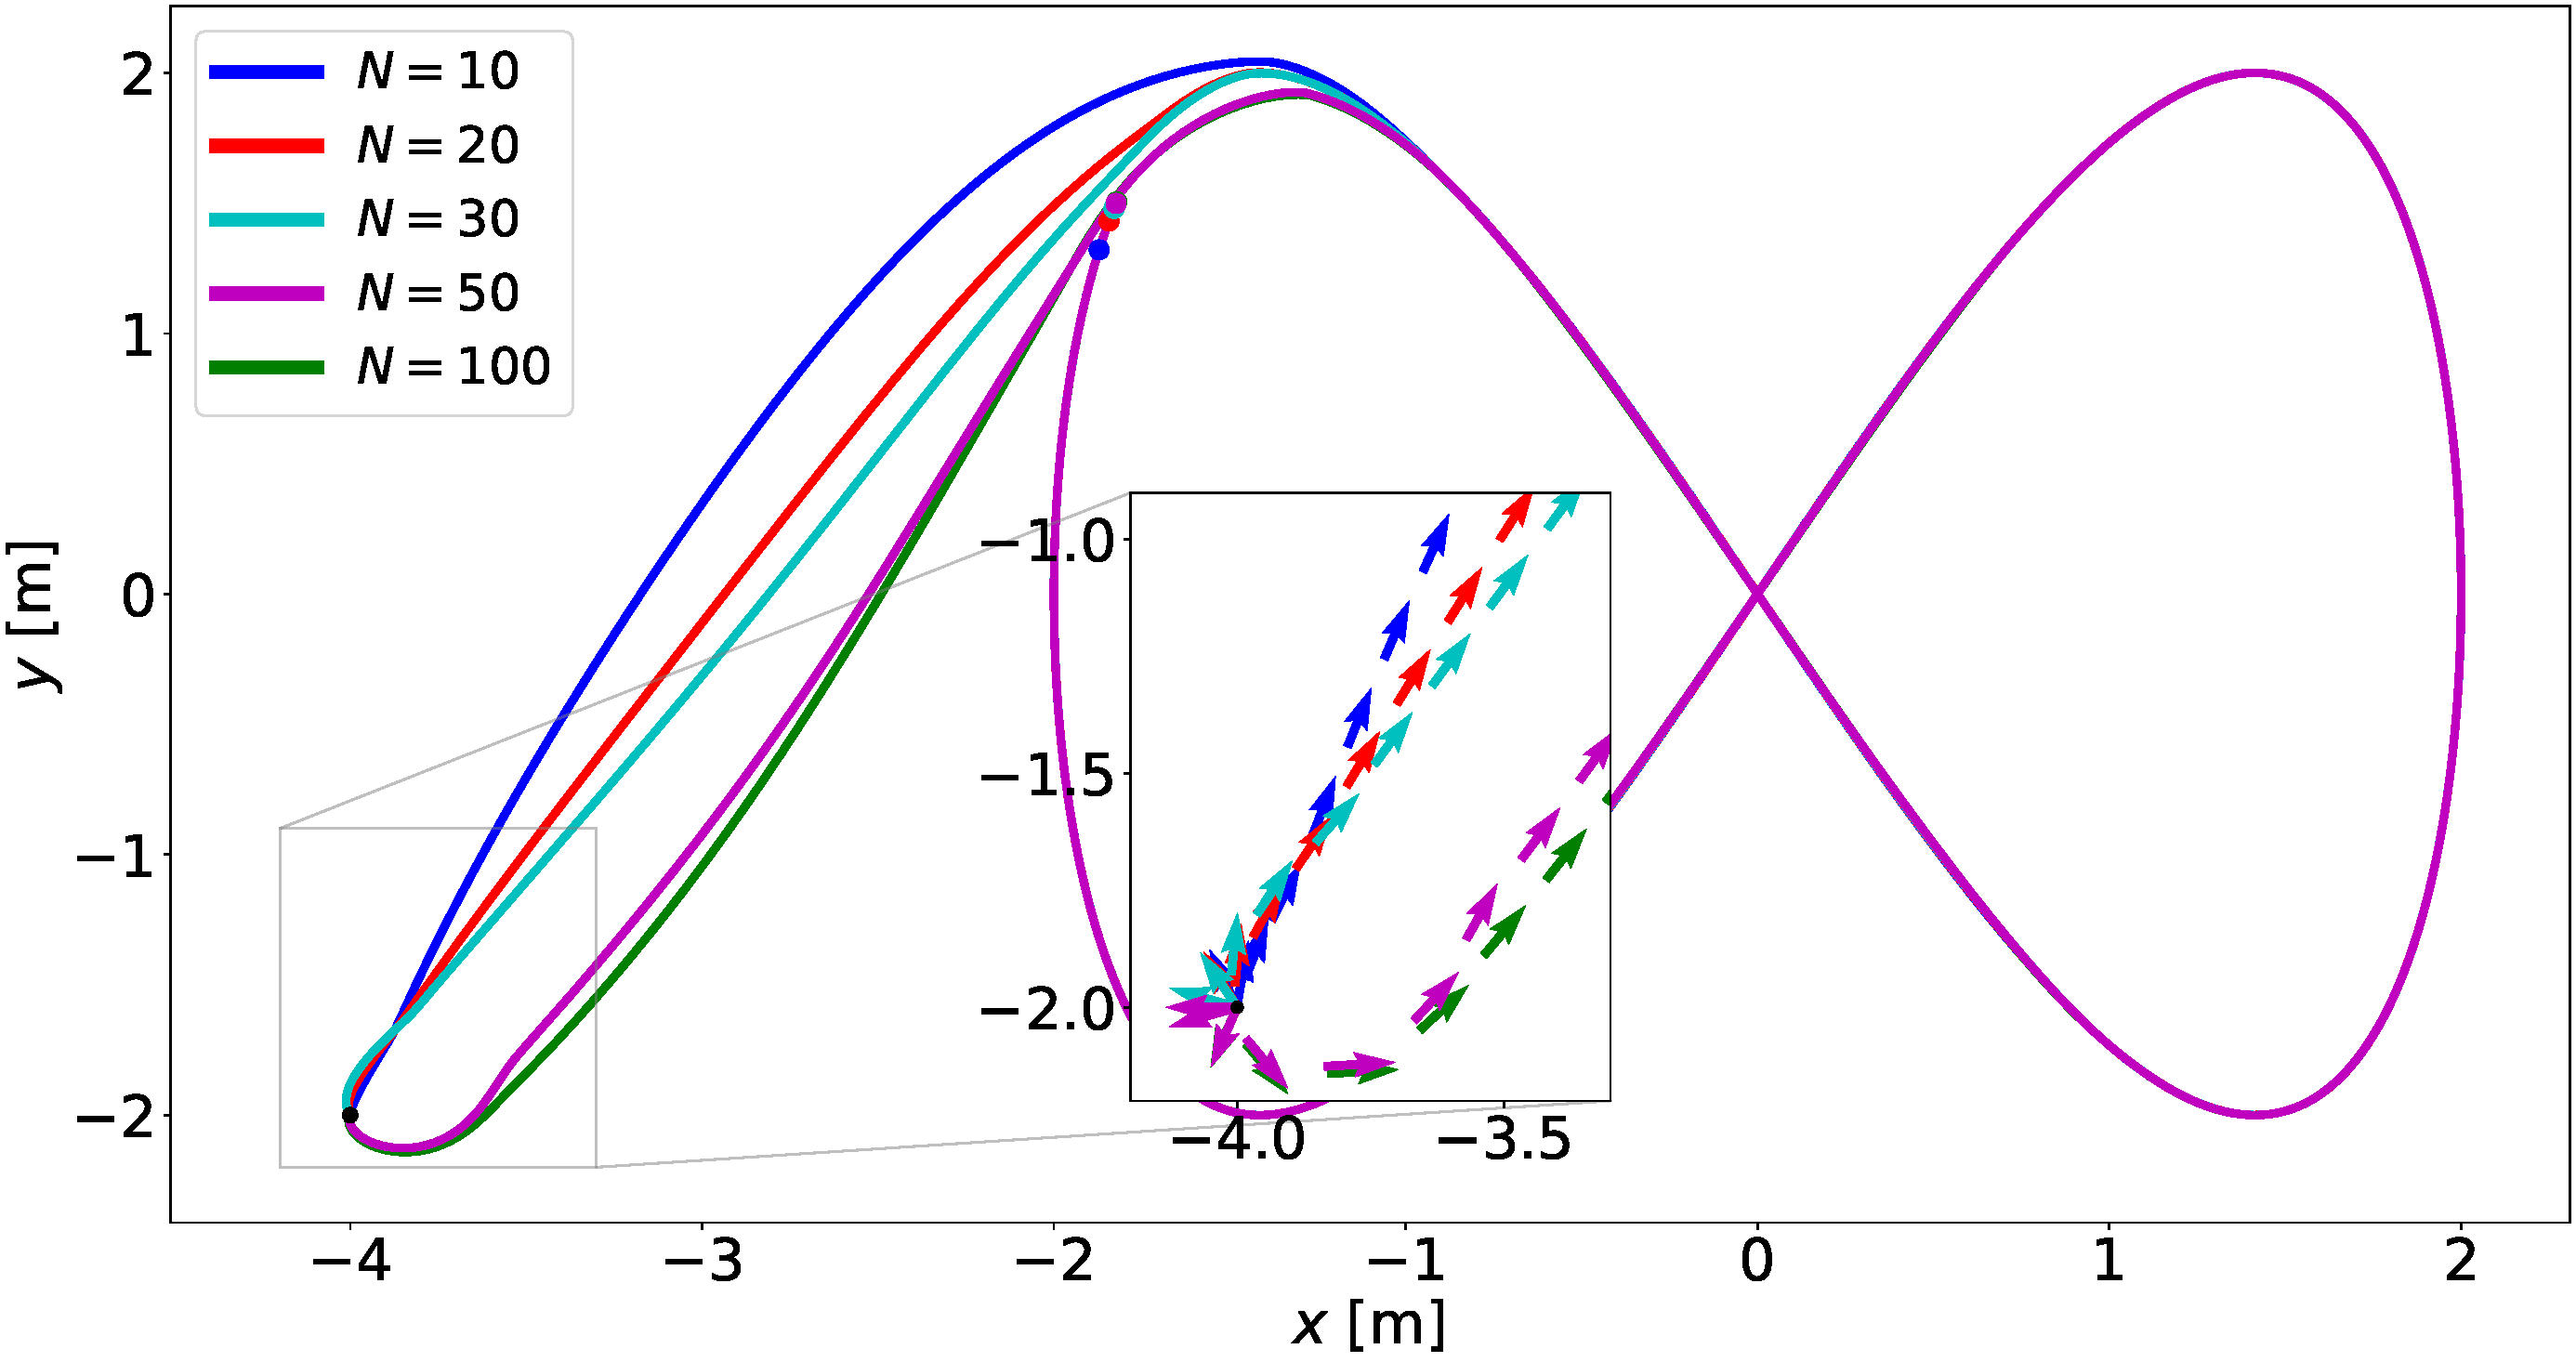
\includegraphics[width=0.48\textwidth]{Figures/One stage OCP/Solver specs comparison/horizon/Virtual speed controlled outside OCP/Planar_onestage_ocp_control_outside_vspeed_comp_horizon.pdf}
        \label{subfig:PathTrackCompHorizonVarOutsideVspeed}
	}
	\caption{Path tracking comparison with control horizon variation.}
	\label{fig:PathTrackCompHorizonVar}
\end{figure}

In all cases, the controllers meet the reference and track it successfully. In the zoomed sections of figure \ref{fig:PathTrackCompHorizonVar}, one can also see that the vehicle turns around from an initial yaw of $-\pi$ to the reference heading and does not move backwards.

The major differences are seen when performance metrics are evaluated. Regarding the cumulative control effort, a clear trend is not identified. However, the cumulative positional error decreases on both architectures as the control horizon increases. The opposite trend is observed with respect to the cumulative heading error. The most significant portions of these two latter cumulative errors come from the first iterations of the simulation. As the control horizon increases, the vehicle catches the reference earlier. That makes the positional error to be smaller, although the heading error is higher. When it comes to progress, it is somewhat the same in all cases, although a smaller progress was recorded when $N=100$ in case the virtual speed is controlled within the \acrshort{nmpc}.

\subsubsection*{Sampling time}

Likewise, the constant parameters are presented in table \ref{tab:samplingTimeSpecs}. The respective results are presented in figure \ref{fig:PathTrackCompSamplingTimeVar} and tables \ref{tab:cumulativeControlEffortSamplingTime}, \ref{tab:cumulativePositionalErrorSamplingTime} and \ref{tab:cumulativeHeadingErrorSamplingTime}.

\begin{table}[!htb]
  \caption[Constant solver parameters when sampling time changes.]{Constant solver parameters.}
  \label{tab:samplingTimeSpecs}
  \renewcommand{\arraystretch}{1.2}
  \centering
  \begin{tabular}[]{ccccccc}
	\toprule
        $Q$ & $R$ & $N$\\
	\midrule
        $diag\left(3.0,\,3.0,\,3.0\right)$ & $diag\left(1\mathrm{e}{-3}
,\, 1\mathrm{e}{-6},\,1\mathrm{e}{-6},\,1\mathrm{e}{-6},\,1\mathrm{e}{-9},\,1\mathrm{e}{-9}\right)$ & $30$\\
	\toprule
		$\left[(v_x)_{min},\; (v_x)_{max}\right]\,[m/s]$ & $\left[(\omega_z)_{min},\; (\omega_z)_{max}\right]\,[rad/s]$ & $\left[v_{min},\;v_{max}\right]$ & $\FrictionCoefficient$\\
	\midrule
		$[0.0,\;2.0]$ & $[-10.0,\;10.0]$ & $[0.0,\;1.0]$ & $1.0$\\
  	\bottomrule
  \end{tabular}
\end{table}

\begin{figure}[!htb]
	\centering
	\subfigure[Controlled virtual speed inside \acrshort{nmpc}]{
        \centering
        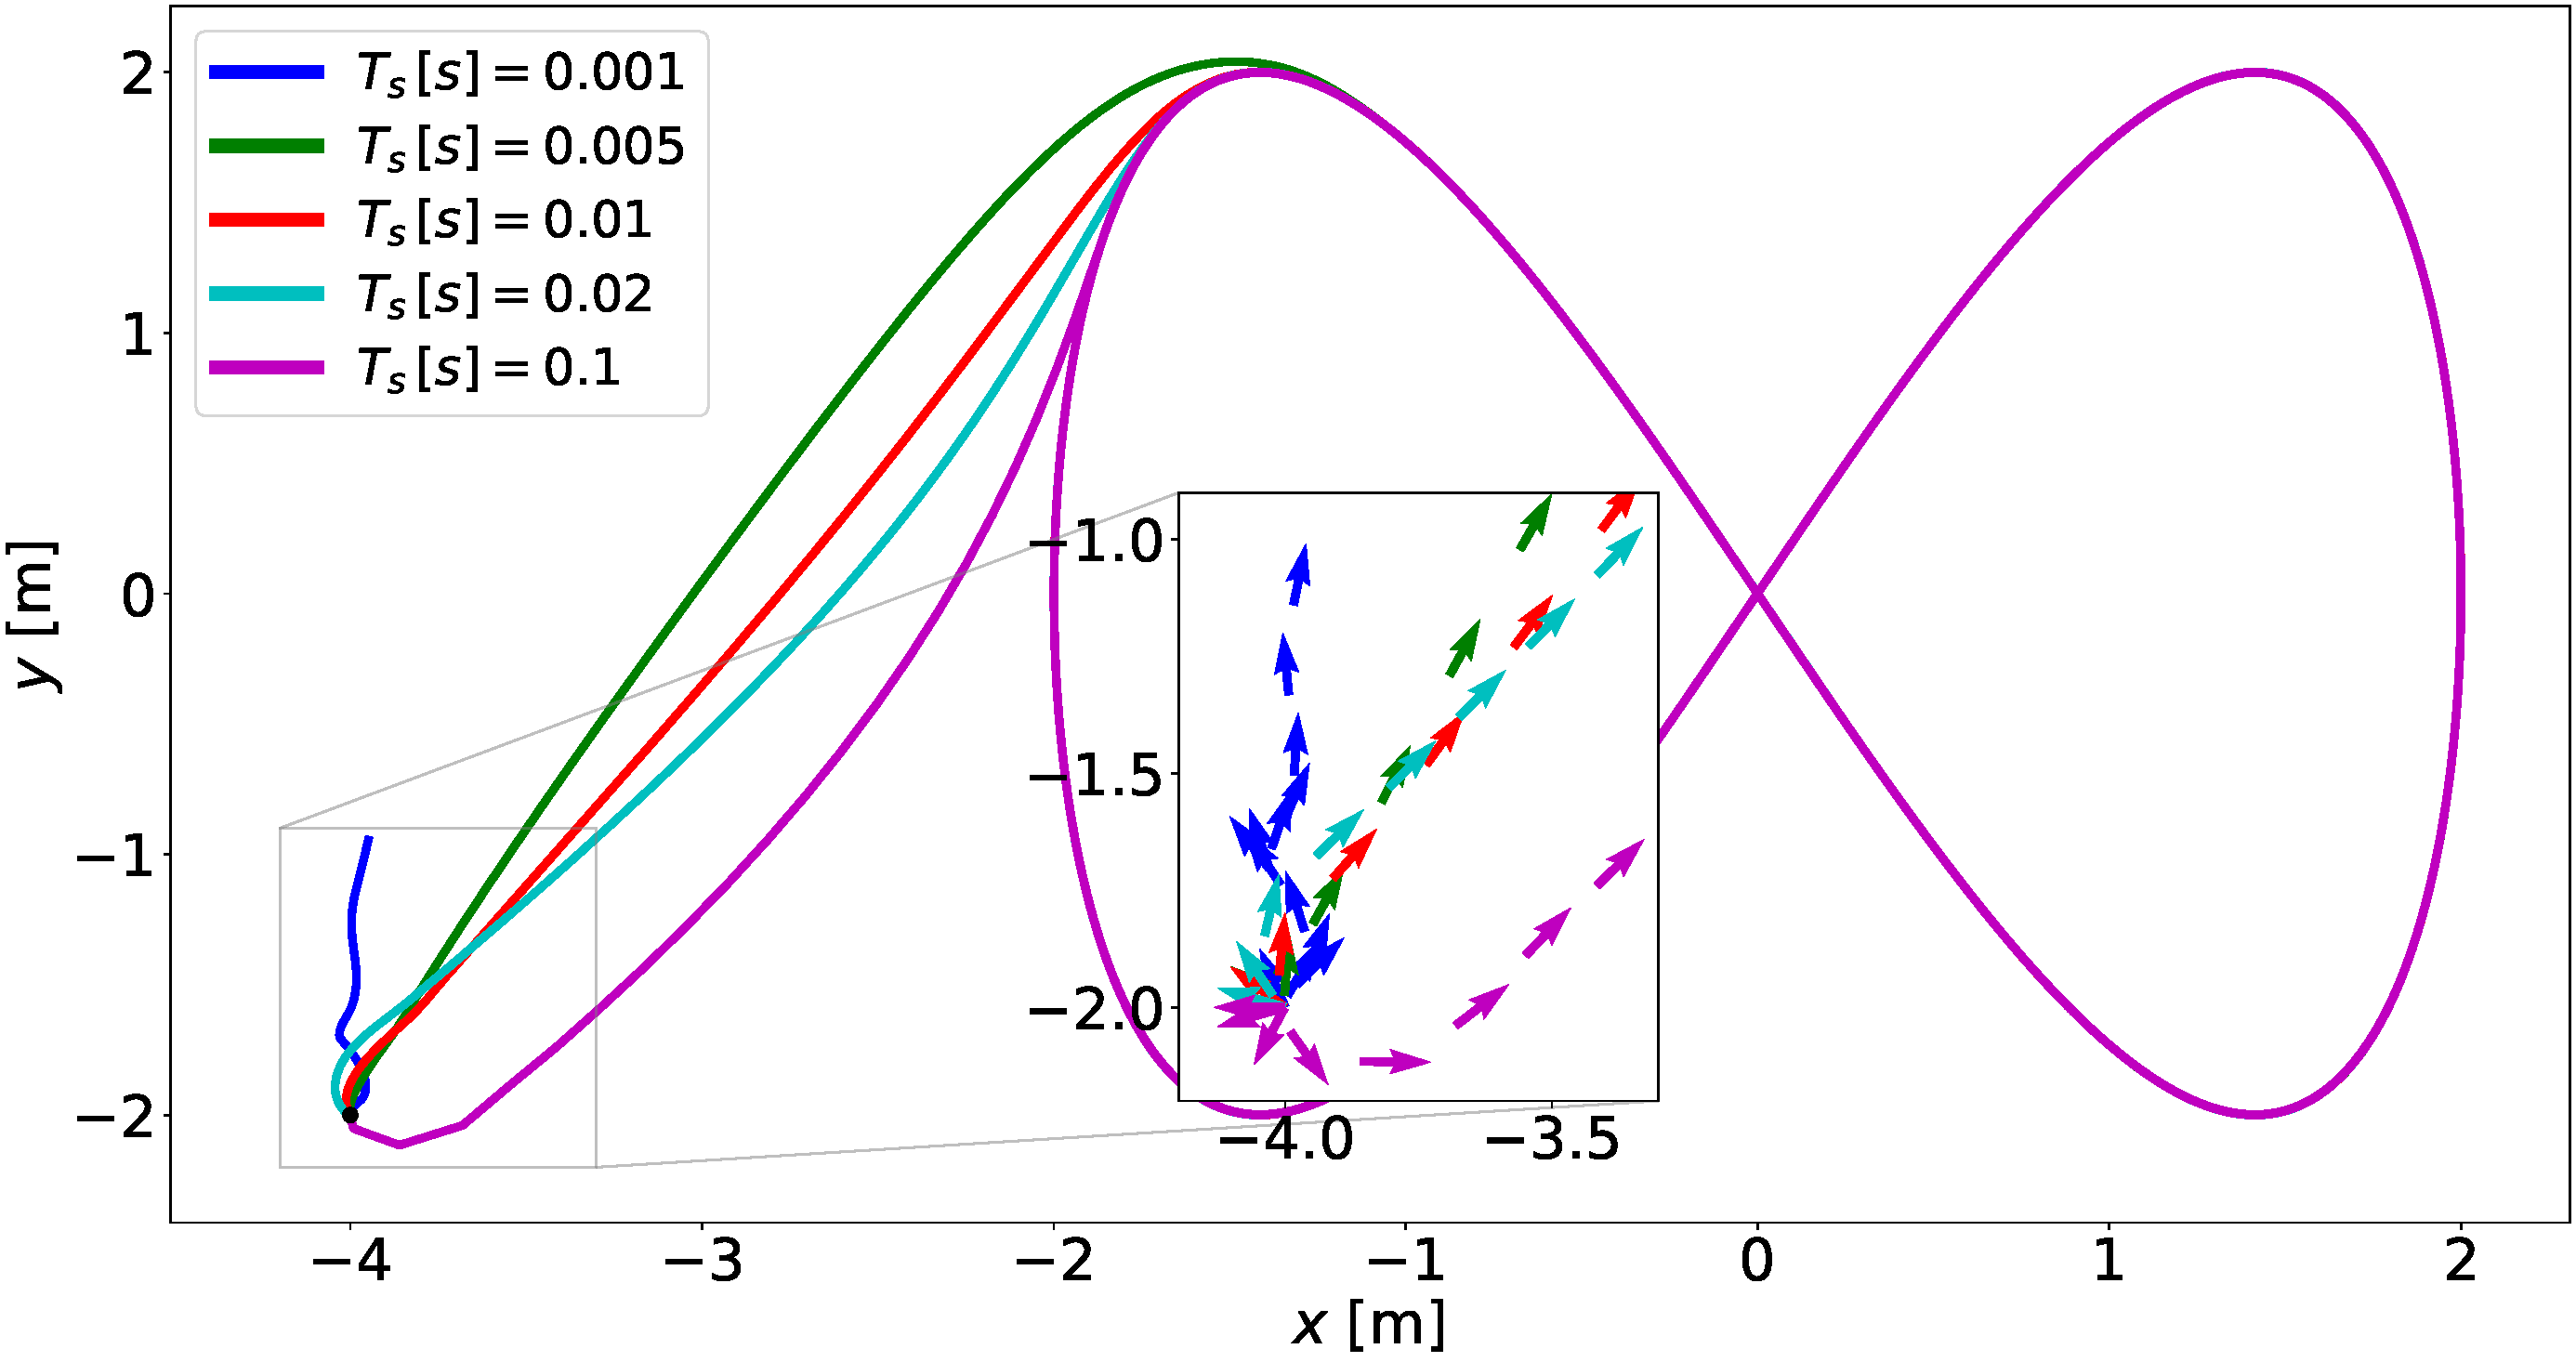
\includegraphics[width=0.48\textwidth]{Figures/One stage OCP/Solver specs comparison/Sampling time/Virtual speed controlled inside OCP/Planar_onestage_ocp_control_vspeed_comp_samplingtime.pdf}
        \label{subfig:PathTrackCompSamplingTimeVarInsideVspeed}
	}
	\hspace{-1.0em}
    \subfigure[Controlled virtual speed outside \acrshort{nmpc}]{
        \centering
        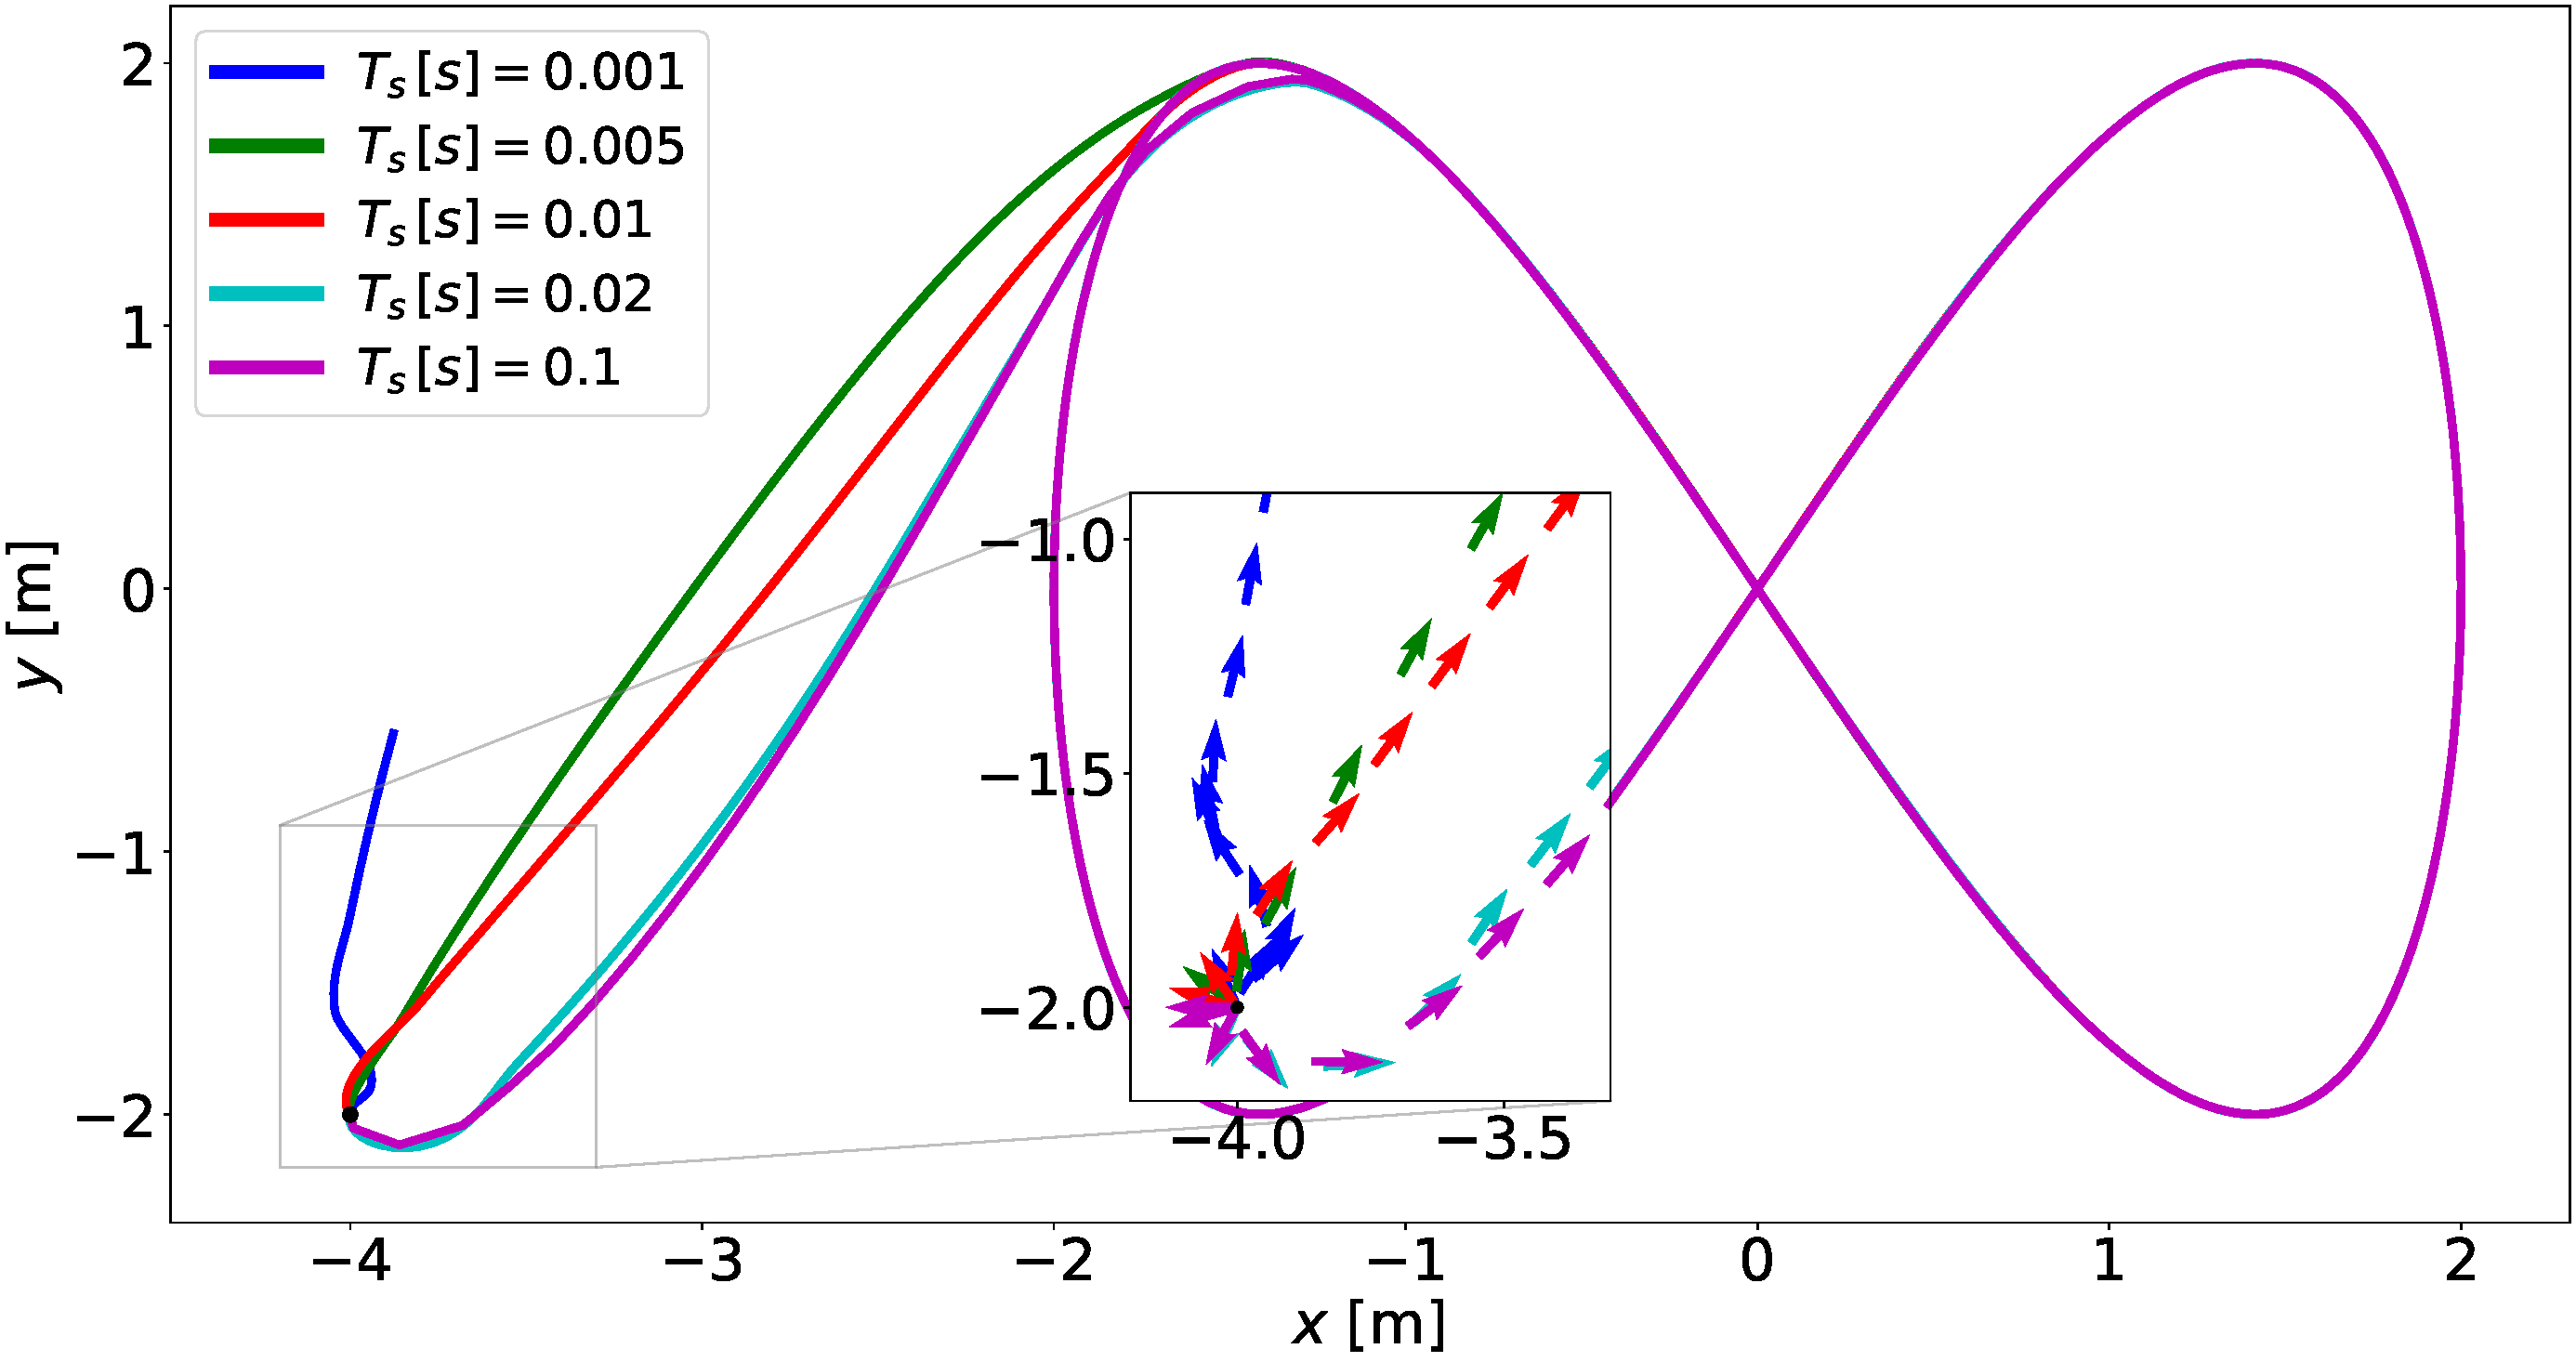
\includegraphics[width=0.48\textwidth]{Figures/One stage OCP/Solver specs comparison/Sampling time/Virtual speed controlled outside OCP/Planar_onestage_ocp_control_outside_vspeed_comp_samplingtime.pdf}
        \label{subfig:PathTrackCompSamplingTimeVarOutsideVspeed}
	}
	\caption{Path tracking comparison with sampling time variation.}
	\label{fig:PathTrackCompSamplingTimeVar}
\end{figure}

All performance metrics are inversely proportional to sampling time. This is due to the fact that higher sampling times increase the time horizon, so the controller may reach the reference sooner and adapt its controls to achieve improved metrics. This is not necessarily the case when the control horizon increases because the number of terms on the cost function increase as well.

Although it seems better performance metrics can be achieved by increasing the sampling time, one should be aware that there is a sampling time floor on a real-time simulation. On one hand, the \textbf{sampling time can't be smaller than the loop time} ($T_c < T_s$). If this rule is violated, there is a great mismatch between the controller's next initial guess and the initial state at the first node of the following iteration. On the other hand, if the sampling time is too big, that mismatch will also happen. In both cases, $\mathbf{x}_{1,\,i-1}^* \nsim \mathbf{\hat{x}}_{0,\,i}$.

\subsubsection*{Cost function weights}
In this segment, the controller is tested against different sets of weights. The control horizon and sampling time remain constant.

\begin{remark}
The cost function of an \acrshort{nmpc} shall pursue the minimization of a single and clearly stated goal. From trial and error experiments, it is not a good practice to seek more than one goal at the same time.
\end{remark}

Based on the previous remark, several types of controllers are set up in table \ref{tab:setsWeights}. Although tracking the reference stands as the main goal, some attention is paid to secondary performance objectives in controllers \textit{Low control effort} and \textit{Smooth controls}. The traversal performed by the vehicle is presented in figure \ref{fig:PathTrackCompWeightsVar}.

\begin{table}[!htb]
  \caption[Constant solver parameters when sampling time changes.]{Solver parameters ($N = 50,\, T_s = 0.01 \, ms$).}
  \label{tab:setsWeights}
  \renewcommand{\arraystretch}{1.2}
  \centering
  \begin{tabular}[]{lcc}
	\toprule
    Type of controller & $Q$ & $R^{\dagger}$\\
	\midrule
    Pose tracker & $diag\left(3.0,\,3.0,\,3.0\right)$ & $diag\left(1\mathrm{e}{-3}
,\, 1\mathrm{e}{-6},\,1\mathrm{e}{-6},\,1\mathrm{e}{-6},\,1\mathrm{e}{-9},\,1\mathrm{e}{-9}\right)$\\
	Position tracker & $diag\left(3.0,\,3.0,\,1.0\right)$ & $diag\left(1\mathrm{e}{-3}
,\, 1\mathrm{e}{-6},\,1\mathrm{e}{-6},\,1\mathrm{e}{-6},\,1\mathrm{e}{-9},\,1\mathrm{e}{-9}\right)$\\
	Heading tracker & $diag\left(1.0,\,1.0,\,3.0\right)$ & $diag\left(1\mathrm{e}{-3}
,\, 1\mathrm{e}{-6},\,1\mathrm{e}{-6},\,1\mathrm{e}{-6},\,1\mathrm{e}{-9},\,1\mathrm{e}{-9}\right)$\\
	Focus on low control effort & $diag\left(1.0,\,1.0,\,1.0\right)$ & $diag\left(1\mathrm{e}{-3}
,\, 1\mathrm{e}{-6},\,1\mathrm{e}{-6},\,1\mathrm{e}{-6},\,1\mathrm{e}{-3},\,1\mathrm{e}{-3}\right)$\\
	Focus on smooth controls & $diag\left(1.0,\,1.0,\,1.0\right)$ & $diag\left(1\mathrm{e}{-3}
,\, 1\mathrm{e}{-3},\,1\mathrm{e}{-3},\,1\mathrm{e}{-3},\,1\mathrm{e}{-9},\,1\mathrm{e}{-9}\right)$\\
	\bottomrule
  	\multicolumn{3}{l}{\footnotesize $\dagger$ When it comes to virtual speed control outside the \acrshort{nmpc}, the respective weights are removed from $R$.}
  \end{tabular}
  \begin{tabular}[]{cccc}
	\toprule
		$\left[(v_x)_{min},\; (v_x)_{max}\right]\,[m/s]$ & $\left[(\omega_z)_{min},\; (\omega_z)_{max}\right]\,[rad/s]$ & $\left[v_{min},\;v_{max}\right]$ & $\FrictionCoefficient$\\
	\midrule
		$[0.0,\;2.0]$ & $[-10.0,\;10.0]$ & $[0.0,\;1.0]$ & $1.0$\\
  	\bottomrule
  \end{tabular}
\end{table}

\begin{figure}[!htb]
	\centering
	\subfigure[Controlled virtual speed inside \acrshort{nmpc}]{
        \centering
        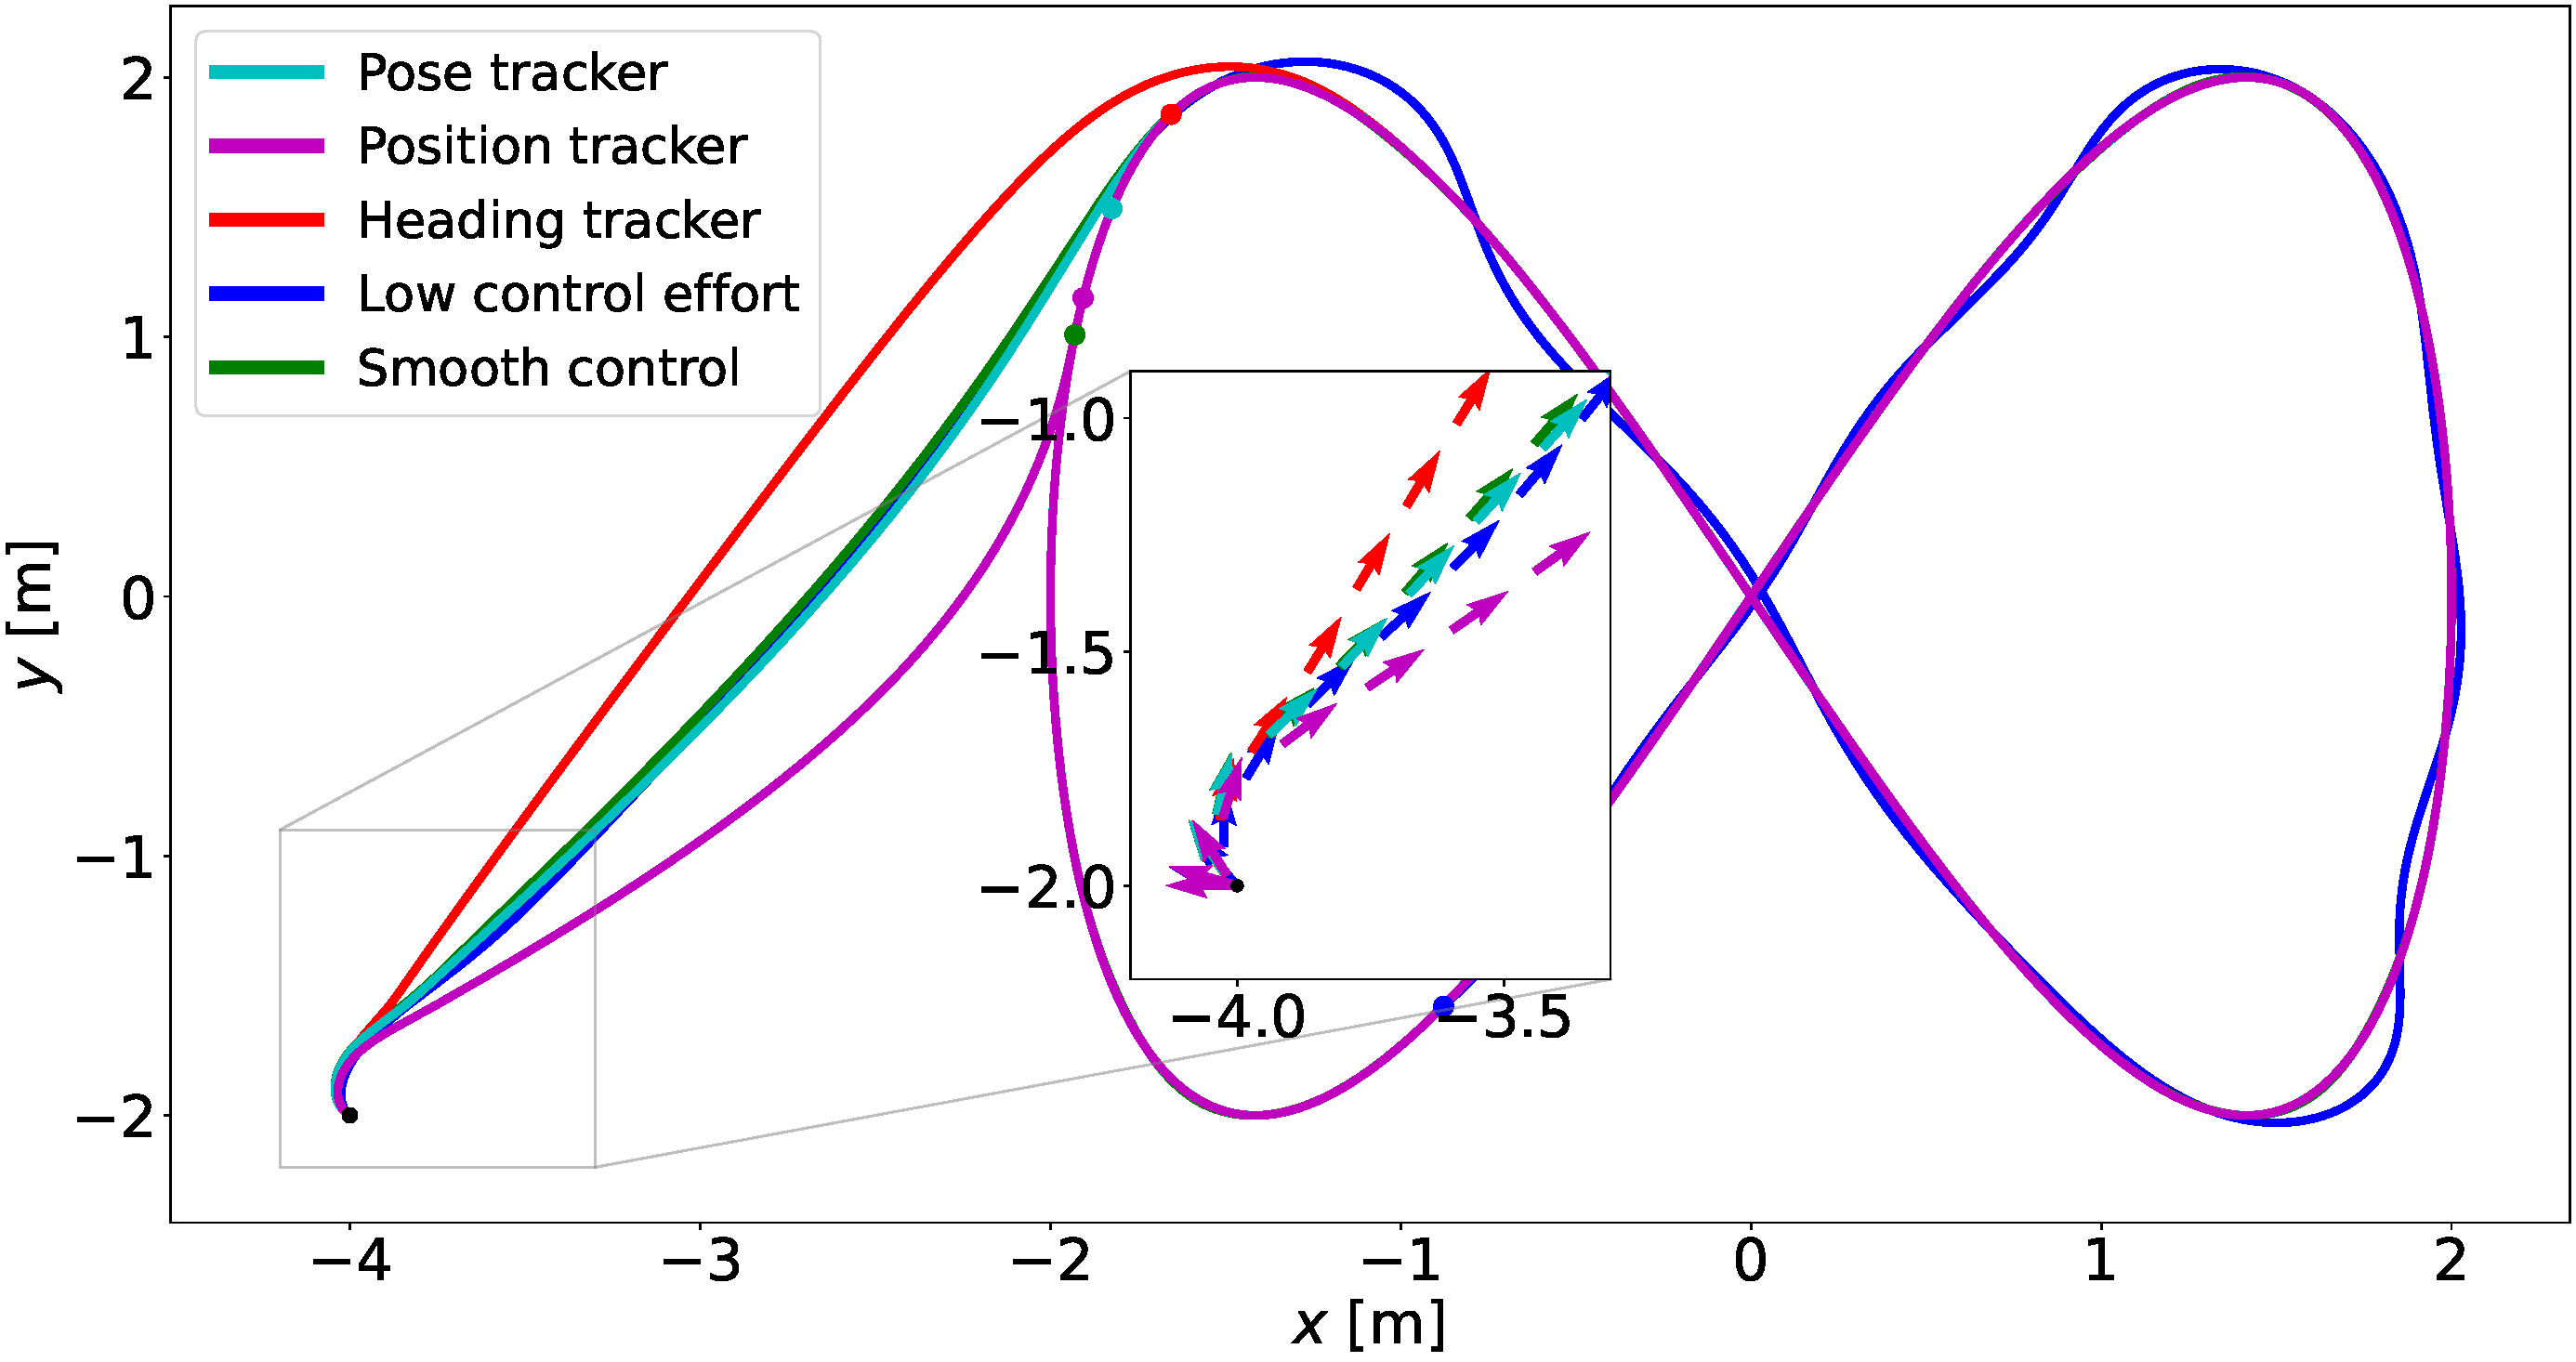
\includegraphics[width=0.48\textwidth]{Figures/One stage OCP/Solver specs comparison/Weights/Virtual speed controlled inside OCP/Planar_onestage_ocp_control_vspeed_comp_weights.pdf}
        \label{subfig:PathTrackCompWeightsVarInsideVspeed}
	}
	\hspace{-1.0em}
    \subfigure[Controlled virtual speed outside \acrshort{nmpc}]{
        \centering
        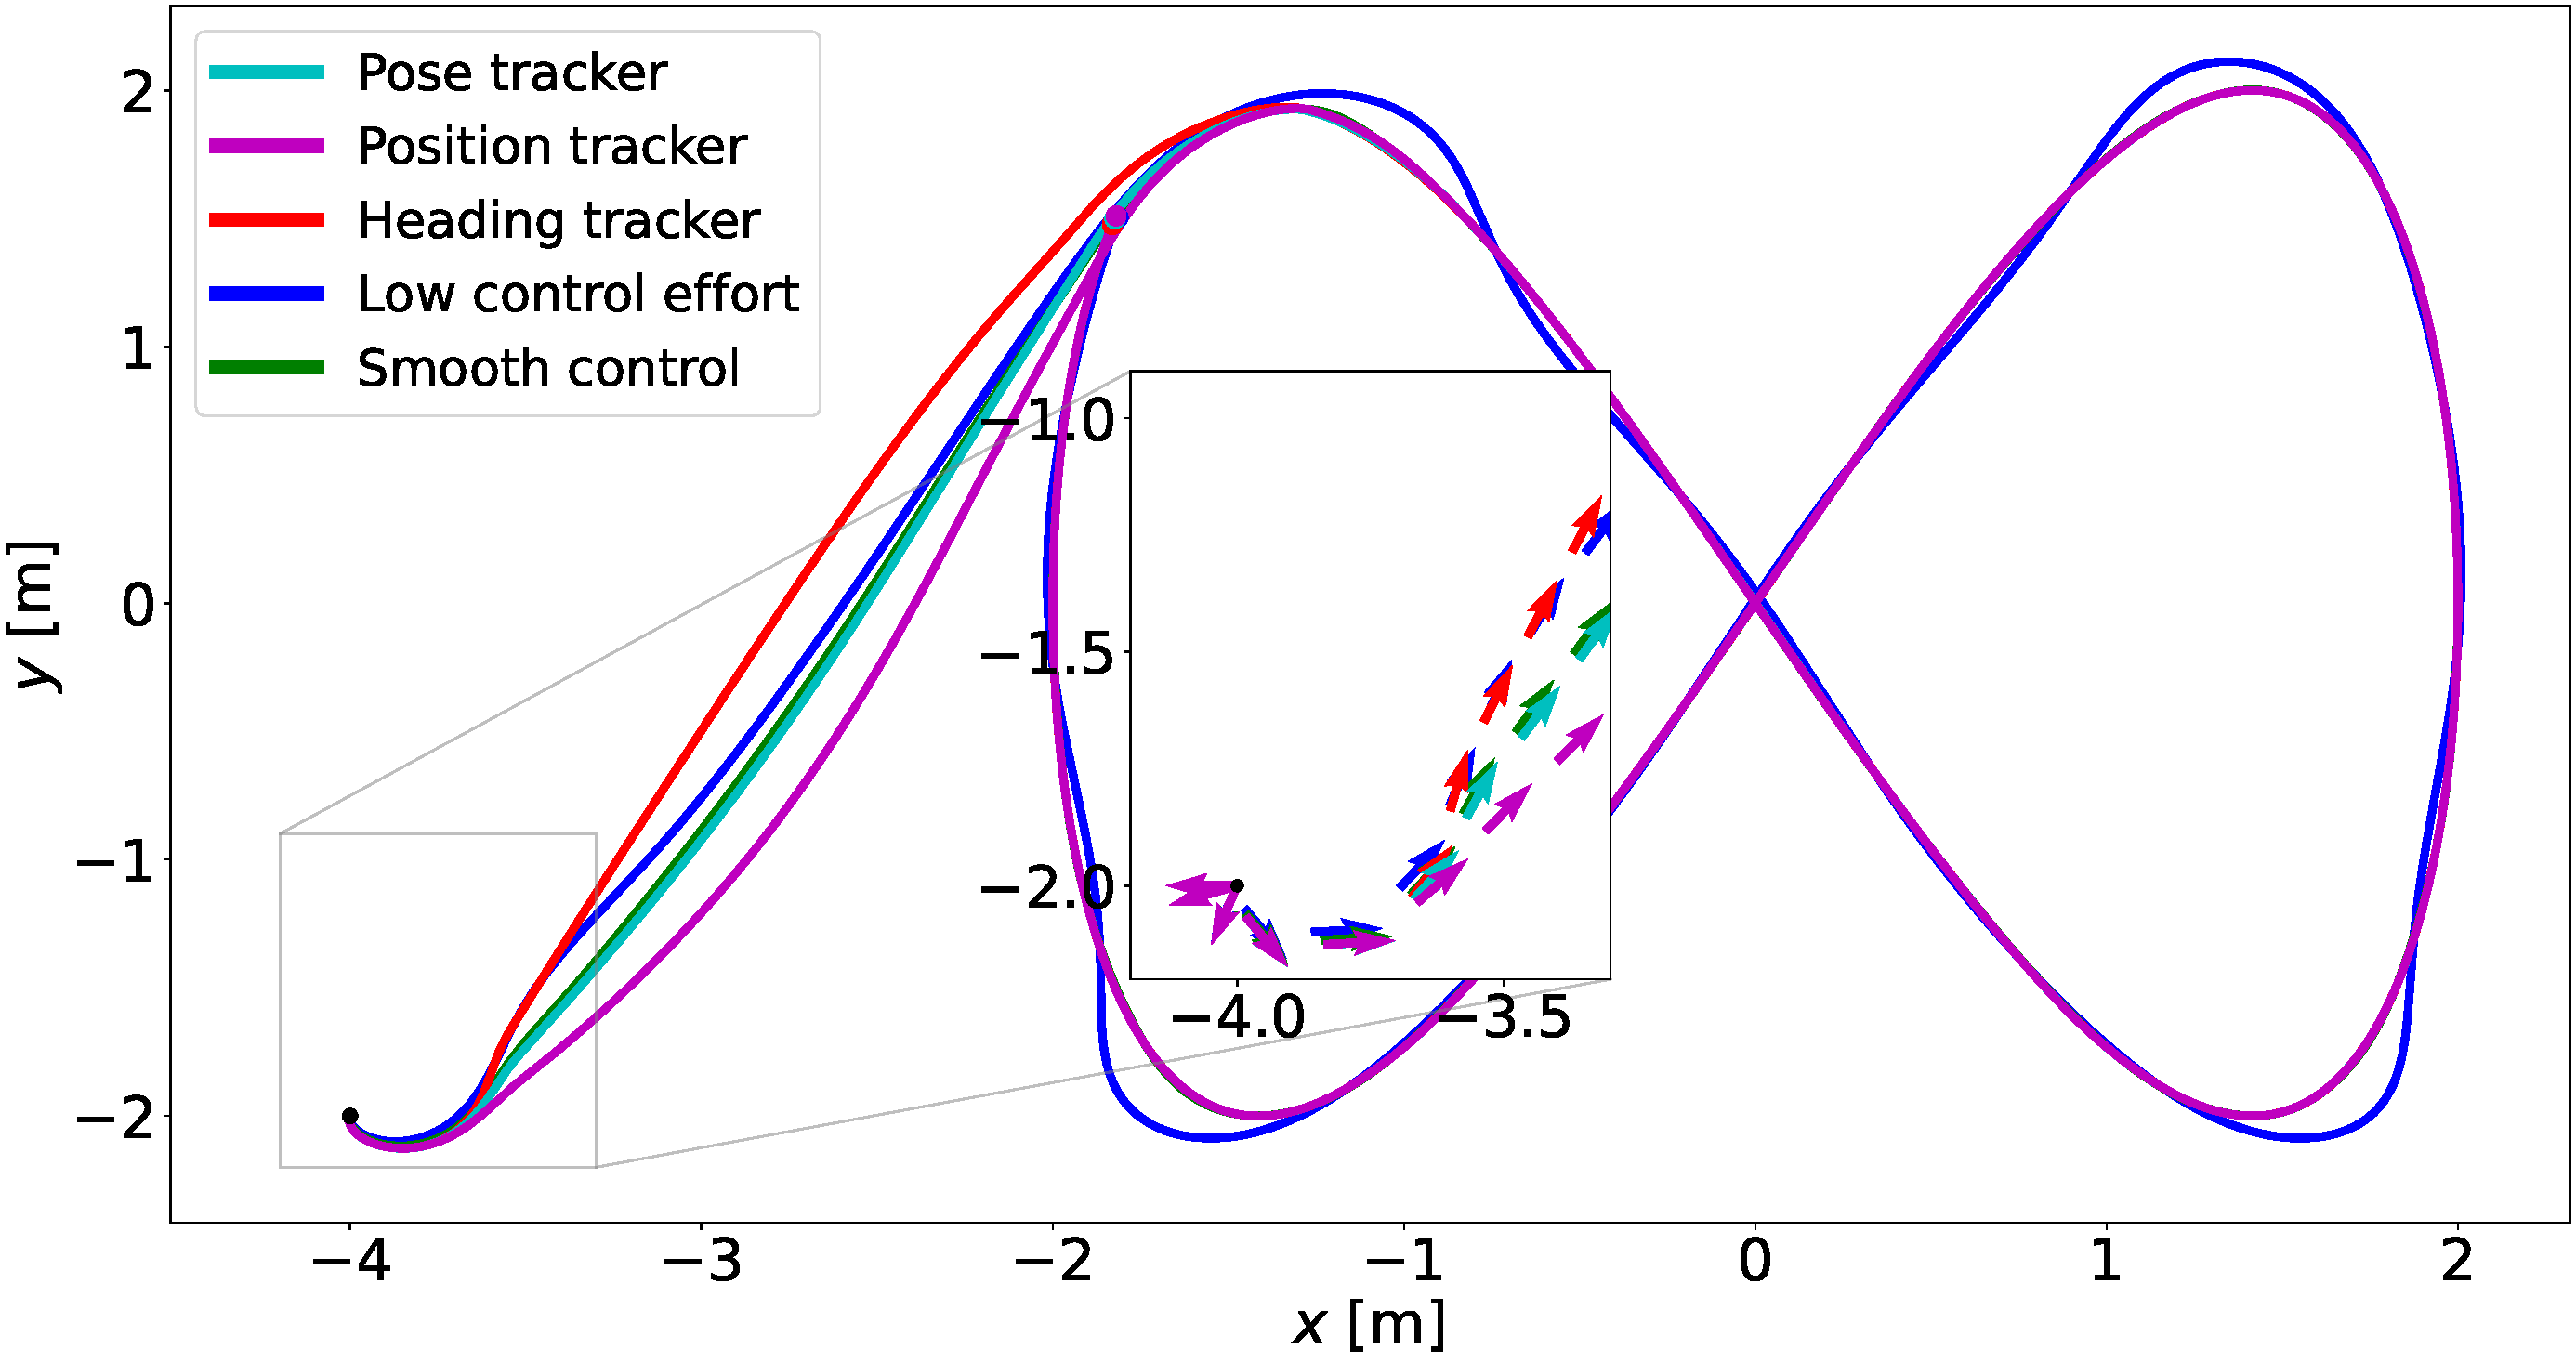
\includegraphics[width=0.48\textwidth]{Figures/One stage OCP/Solver specs comparison/Weights/Virtual speed controlled outside OCP/Planar_onestage_ocp_control_outside_vspeed_comp_weights.pdf}
        \label{subfig:PathTrackCompWeightsVarOutsideVspeed}
	}
	\caption{Path tracking comparison among types of controllers.}
	\label{fig:PathTrackCompWeightsVar}
\end{figure}

For the sake of brevity and simplicity, only the output of $\Traction_l$ and $\Traction_r$ from controllers \textit{Low control effort} and \textit{Smooth controls} is presented in figures \ref{fig:PathTrackCompWeightsVar_tl_limited} and \ref{fig:PathTrackCompWeightsVar_tr_limited}. Data relative to all states and controls on every controller is assembled in figures \ref{fig:PathTrackCompWeightsVar_vx}, \ref{fig:PathTrackCompWeightsVar_wz}, \ref{fig:PathTrackCompWeightsVar_tl} and \ref{fig:PathTrackCompWeightsVar_tr}.

\begin{figure}[!htb]
	\centering
	\subfigure[Controlled virtual speed inside \acrshort{nmpc}]{
        \centering
        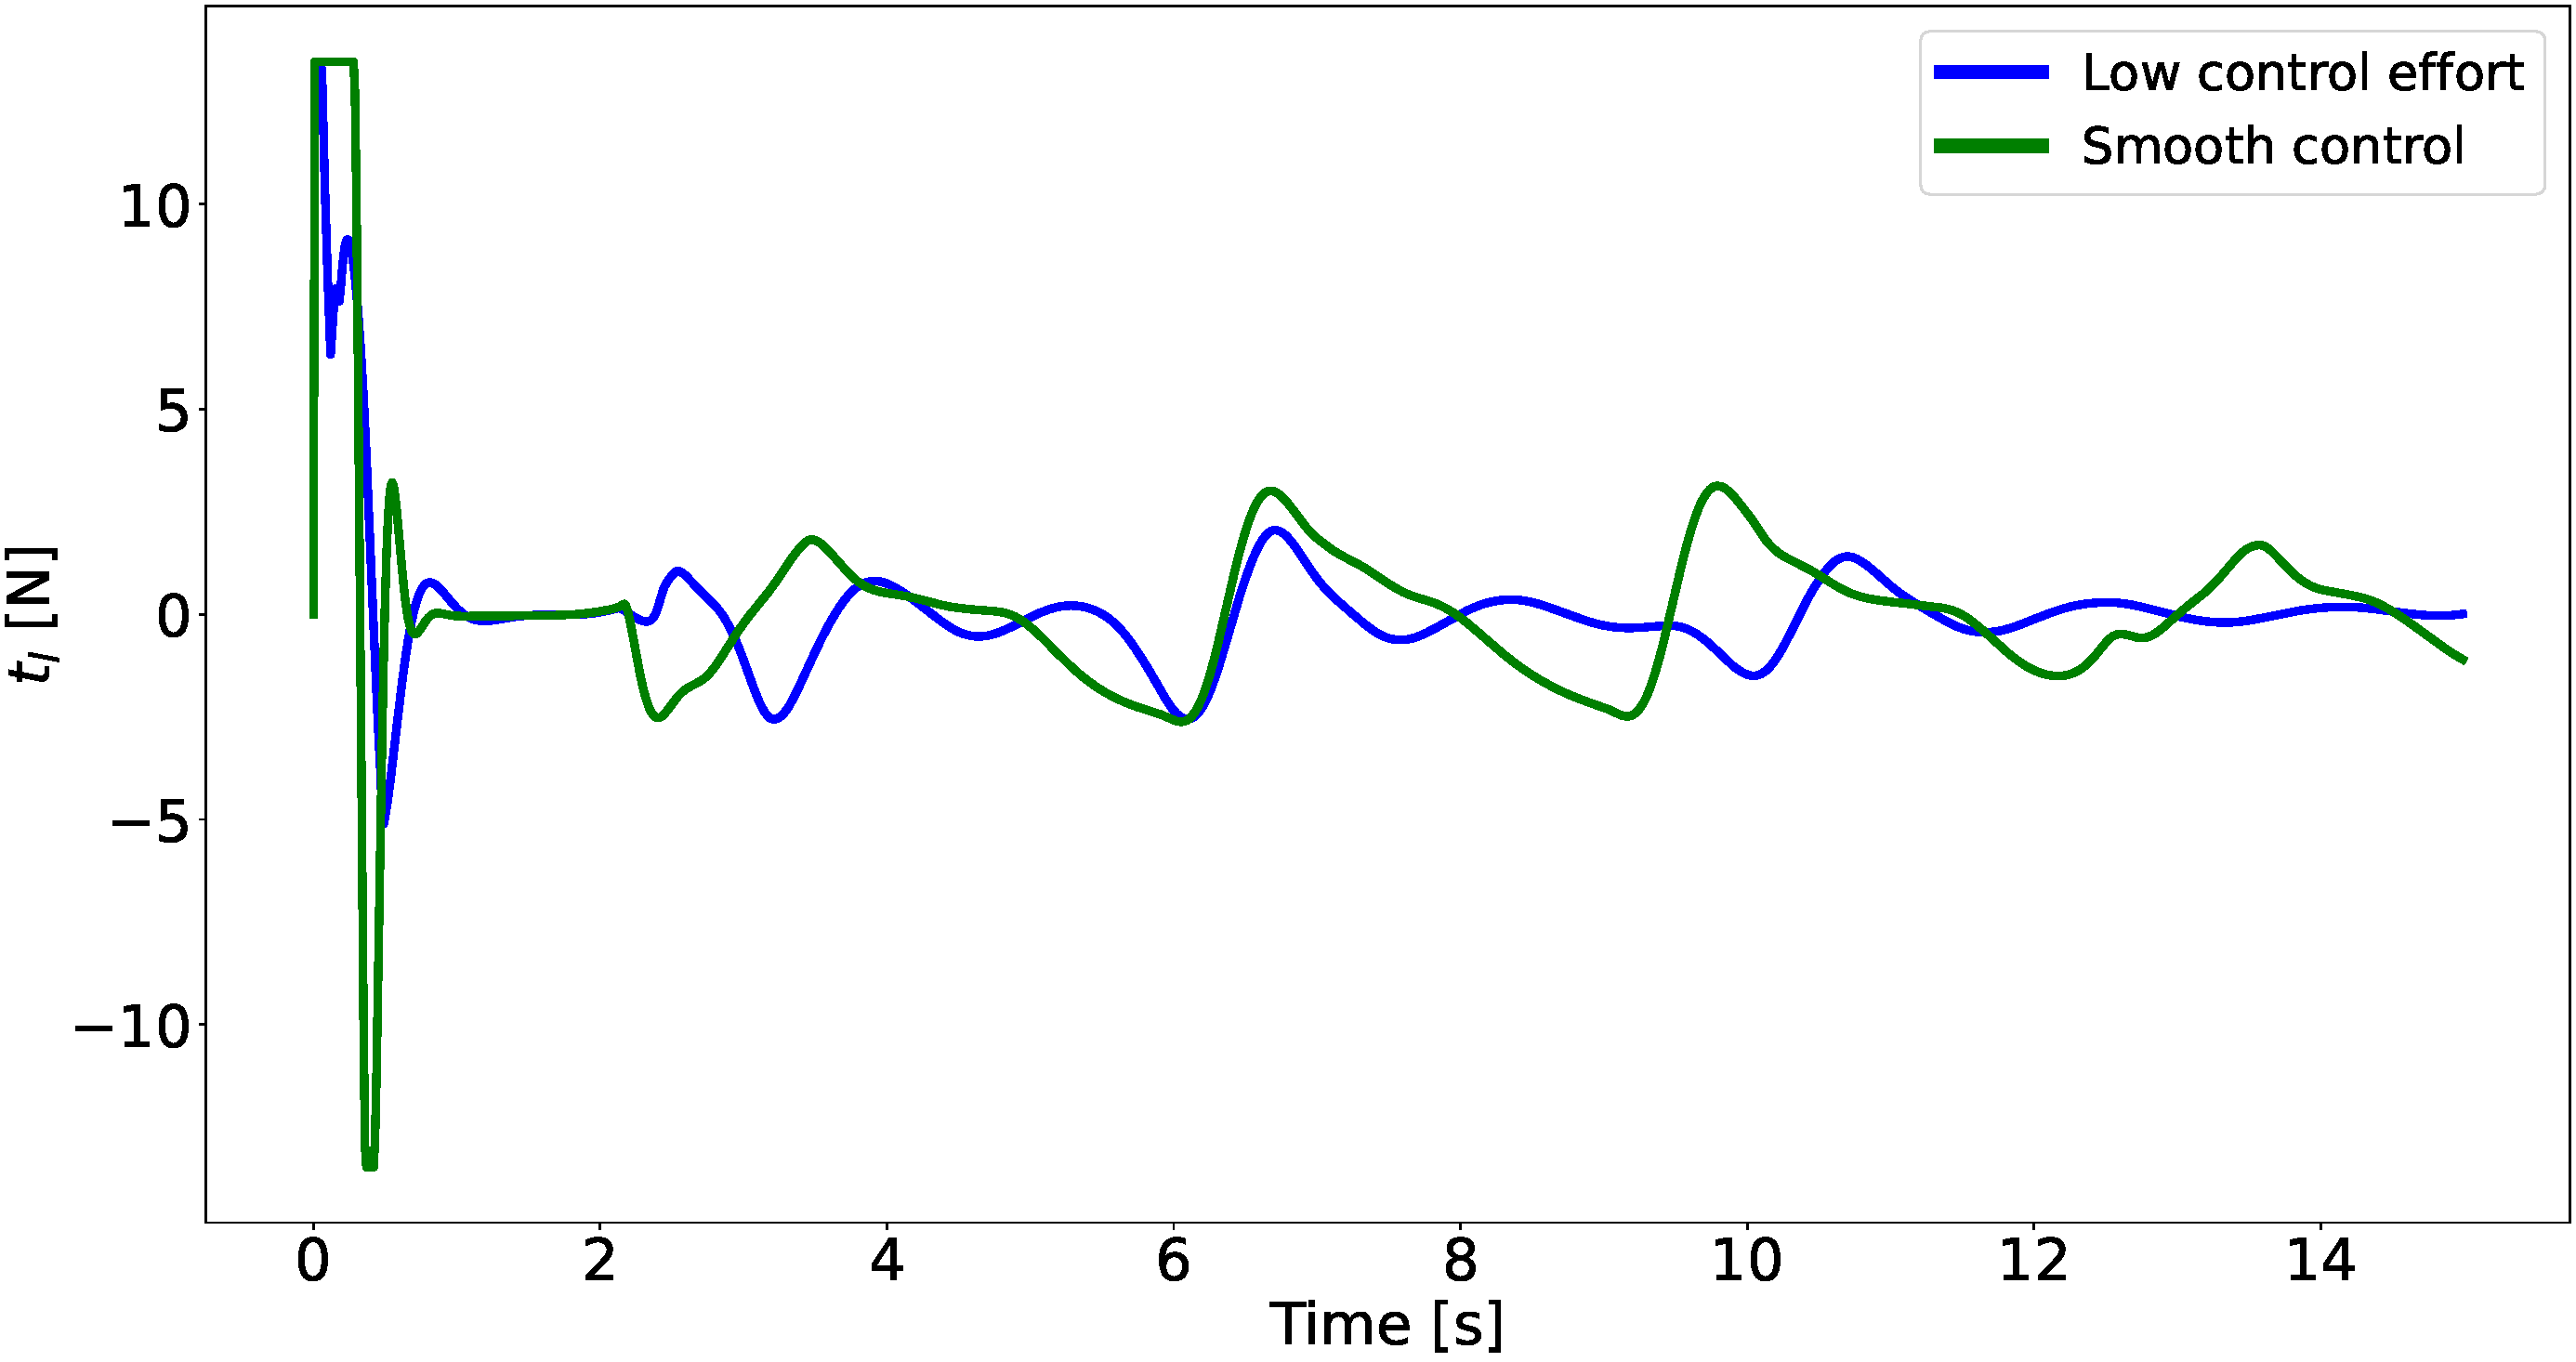
\includegraphics[width=0.48\textwidth]{Figures/One stage OCP/Solver specs comparison/Weights/Virtual speed controlled inside OCP/Planar_onestage_ocp_control_vspeed_comp_tl_limited_weights.pdf}
        \label{subfig:PathTrackCompWeightsVarInsideVspeed_tl}
	}
	\hspace{-1.0em}
    \subfigure[Controlled virtual speed outside \acrshort{nmpc}]{
        \centering
        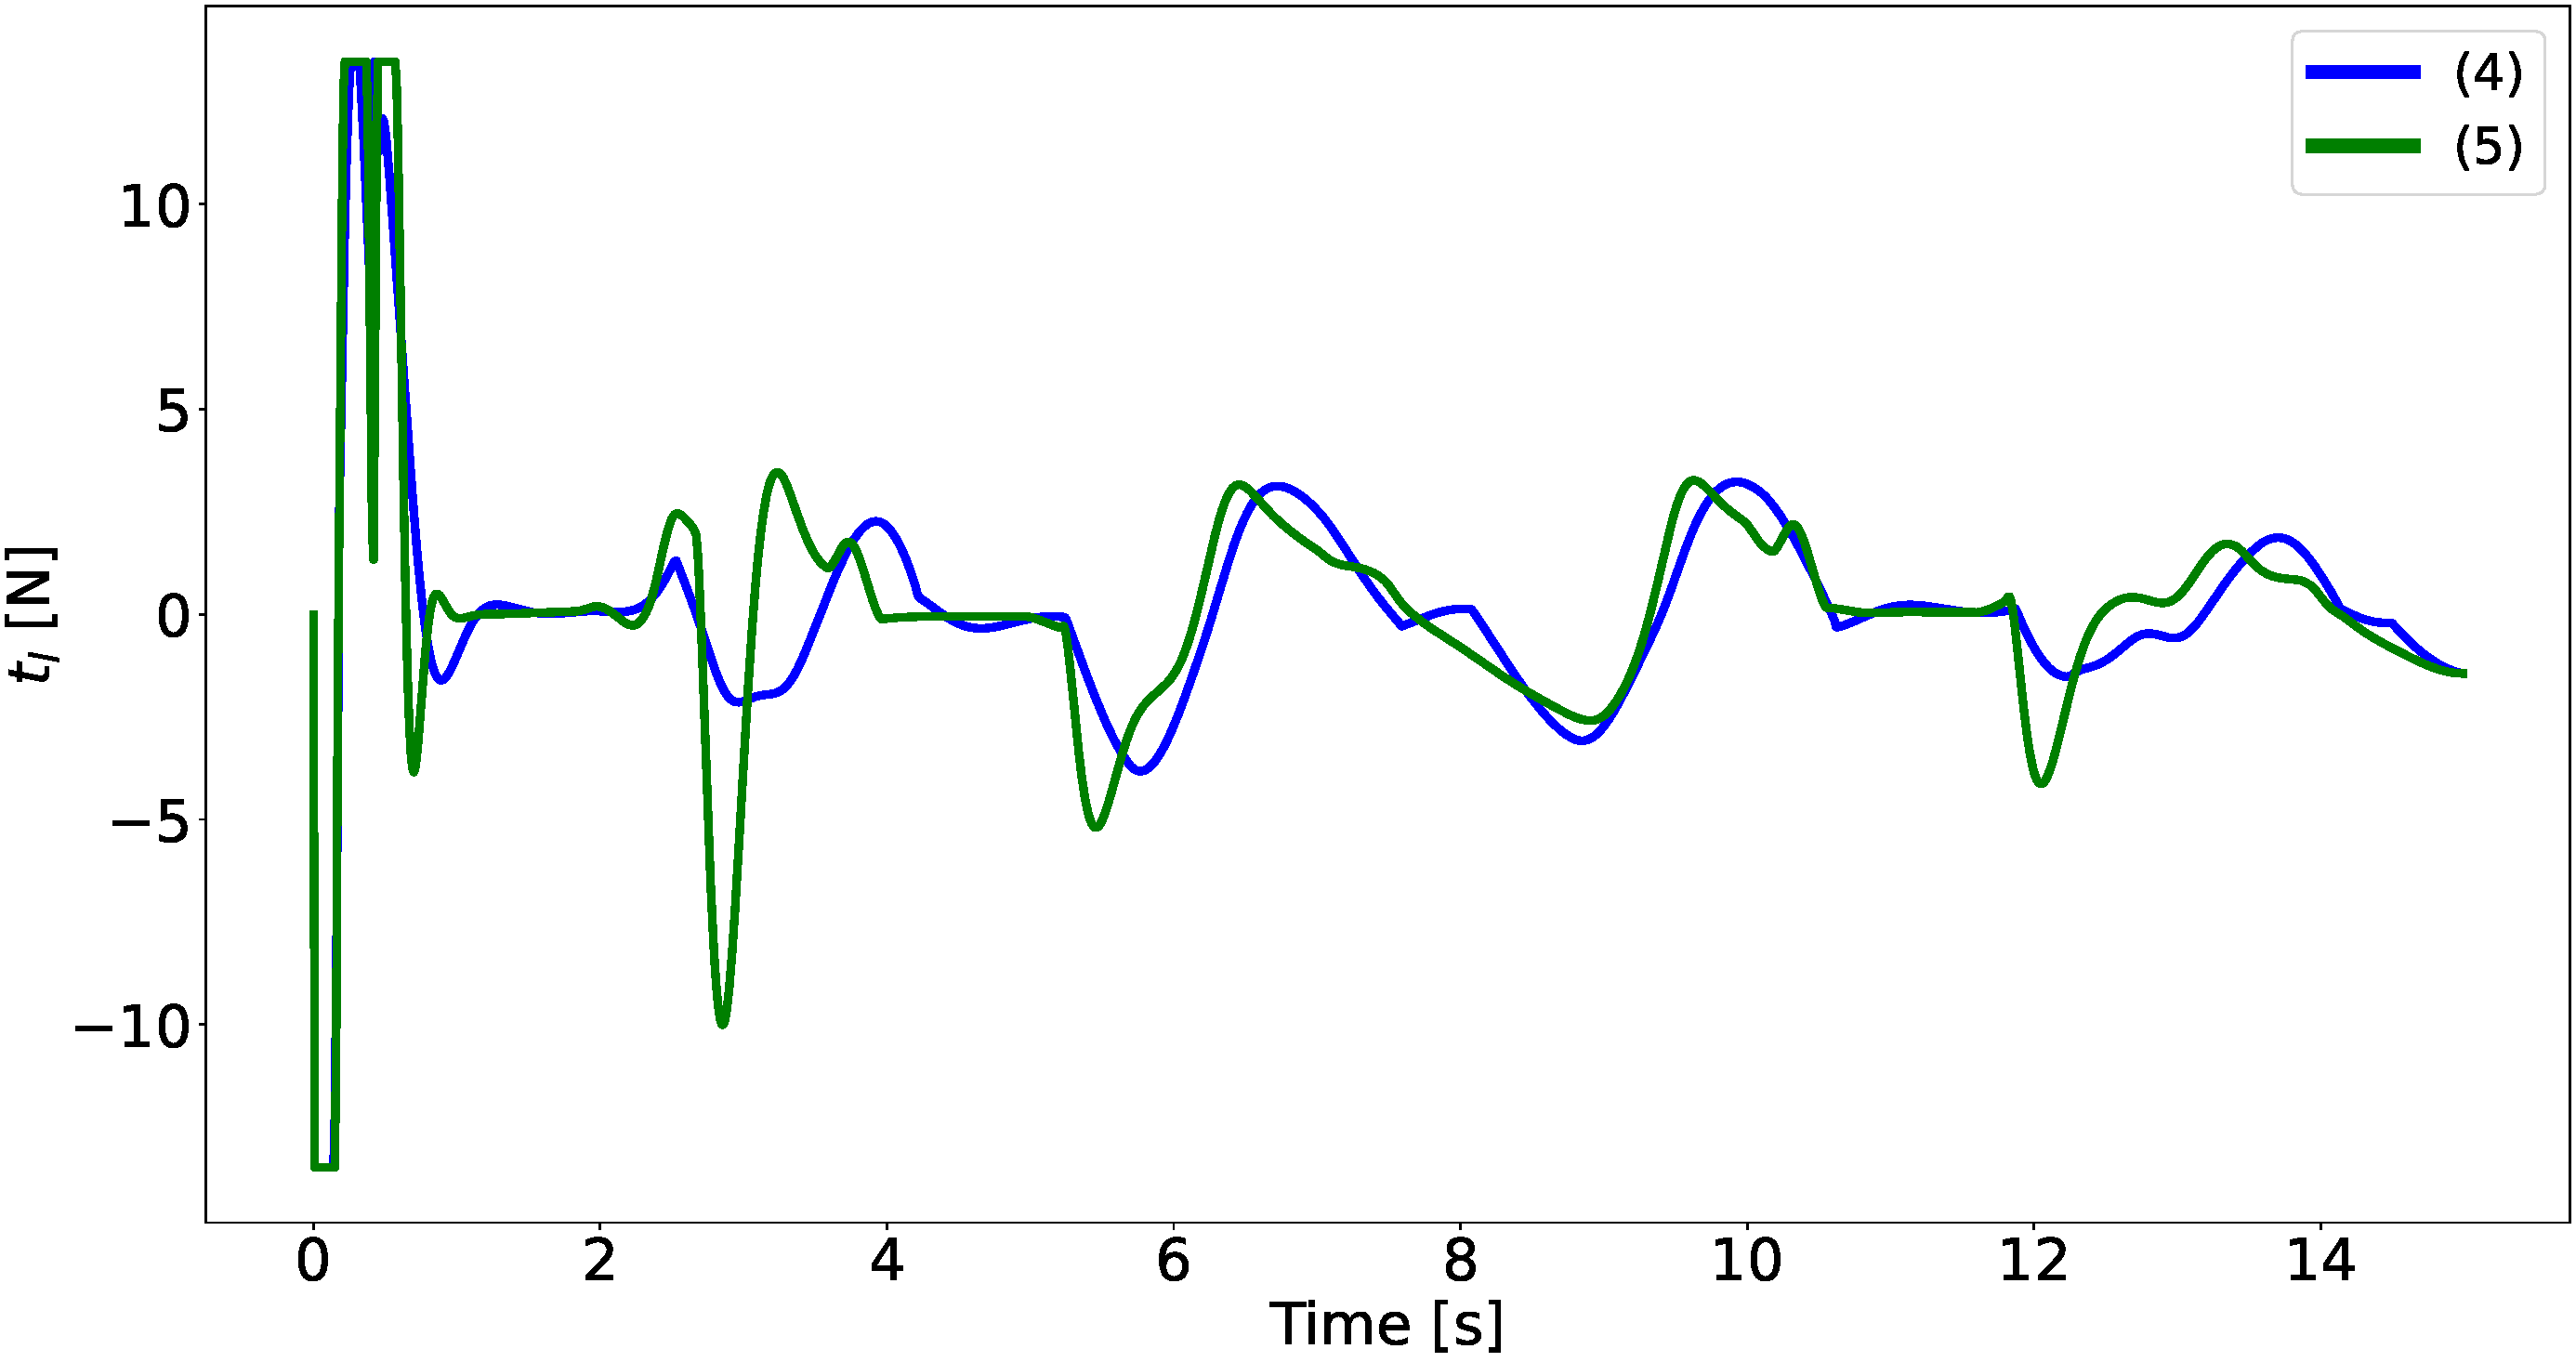
\includegraphics[width=0.48\textwidth]{Figures/One stage OCP/Solver specs comparison/Weights/Virtual speed controlled outside OCP/Planar_onestage_ocp_control_outside_vspeed_comp_tl_limited_weights.pdf}
        \label{subfig:PathTrackCompWeightsVarOutsideVspeed_tl}
	}
	\caption{$\Traction_l$ curve comparison between controllers \textit{Low control effort} and \textit{Smooth control}.}
	\label{fig:PathTrackCompWeightsVar_tl_limited}
\end{figure}

\begin{figure}[!htb]
	\centering
	\subfigure[Controlled virtual speed inside \acrshort{nmpc}]{
        \centering
        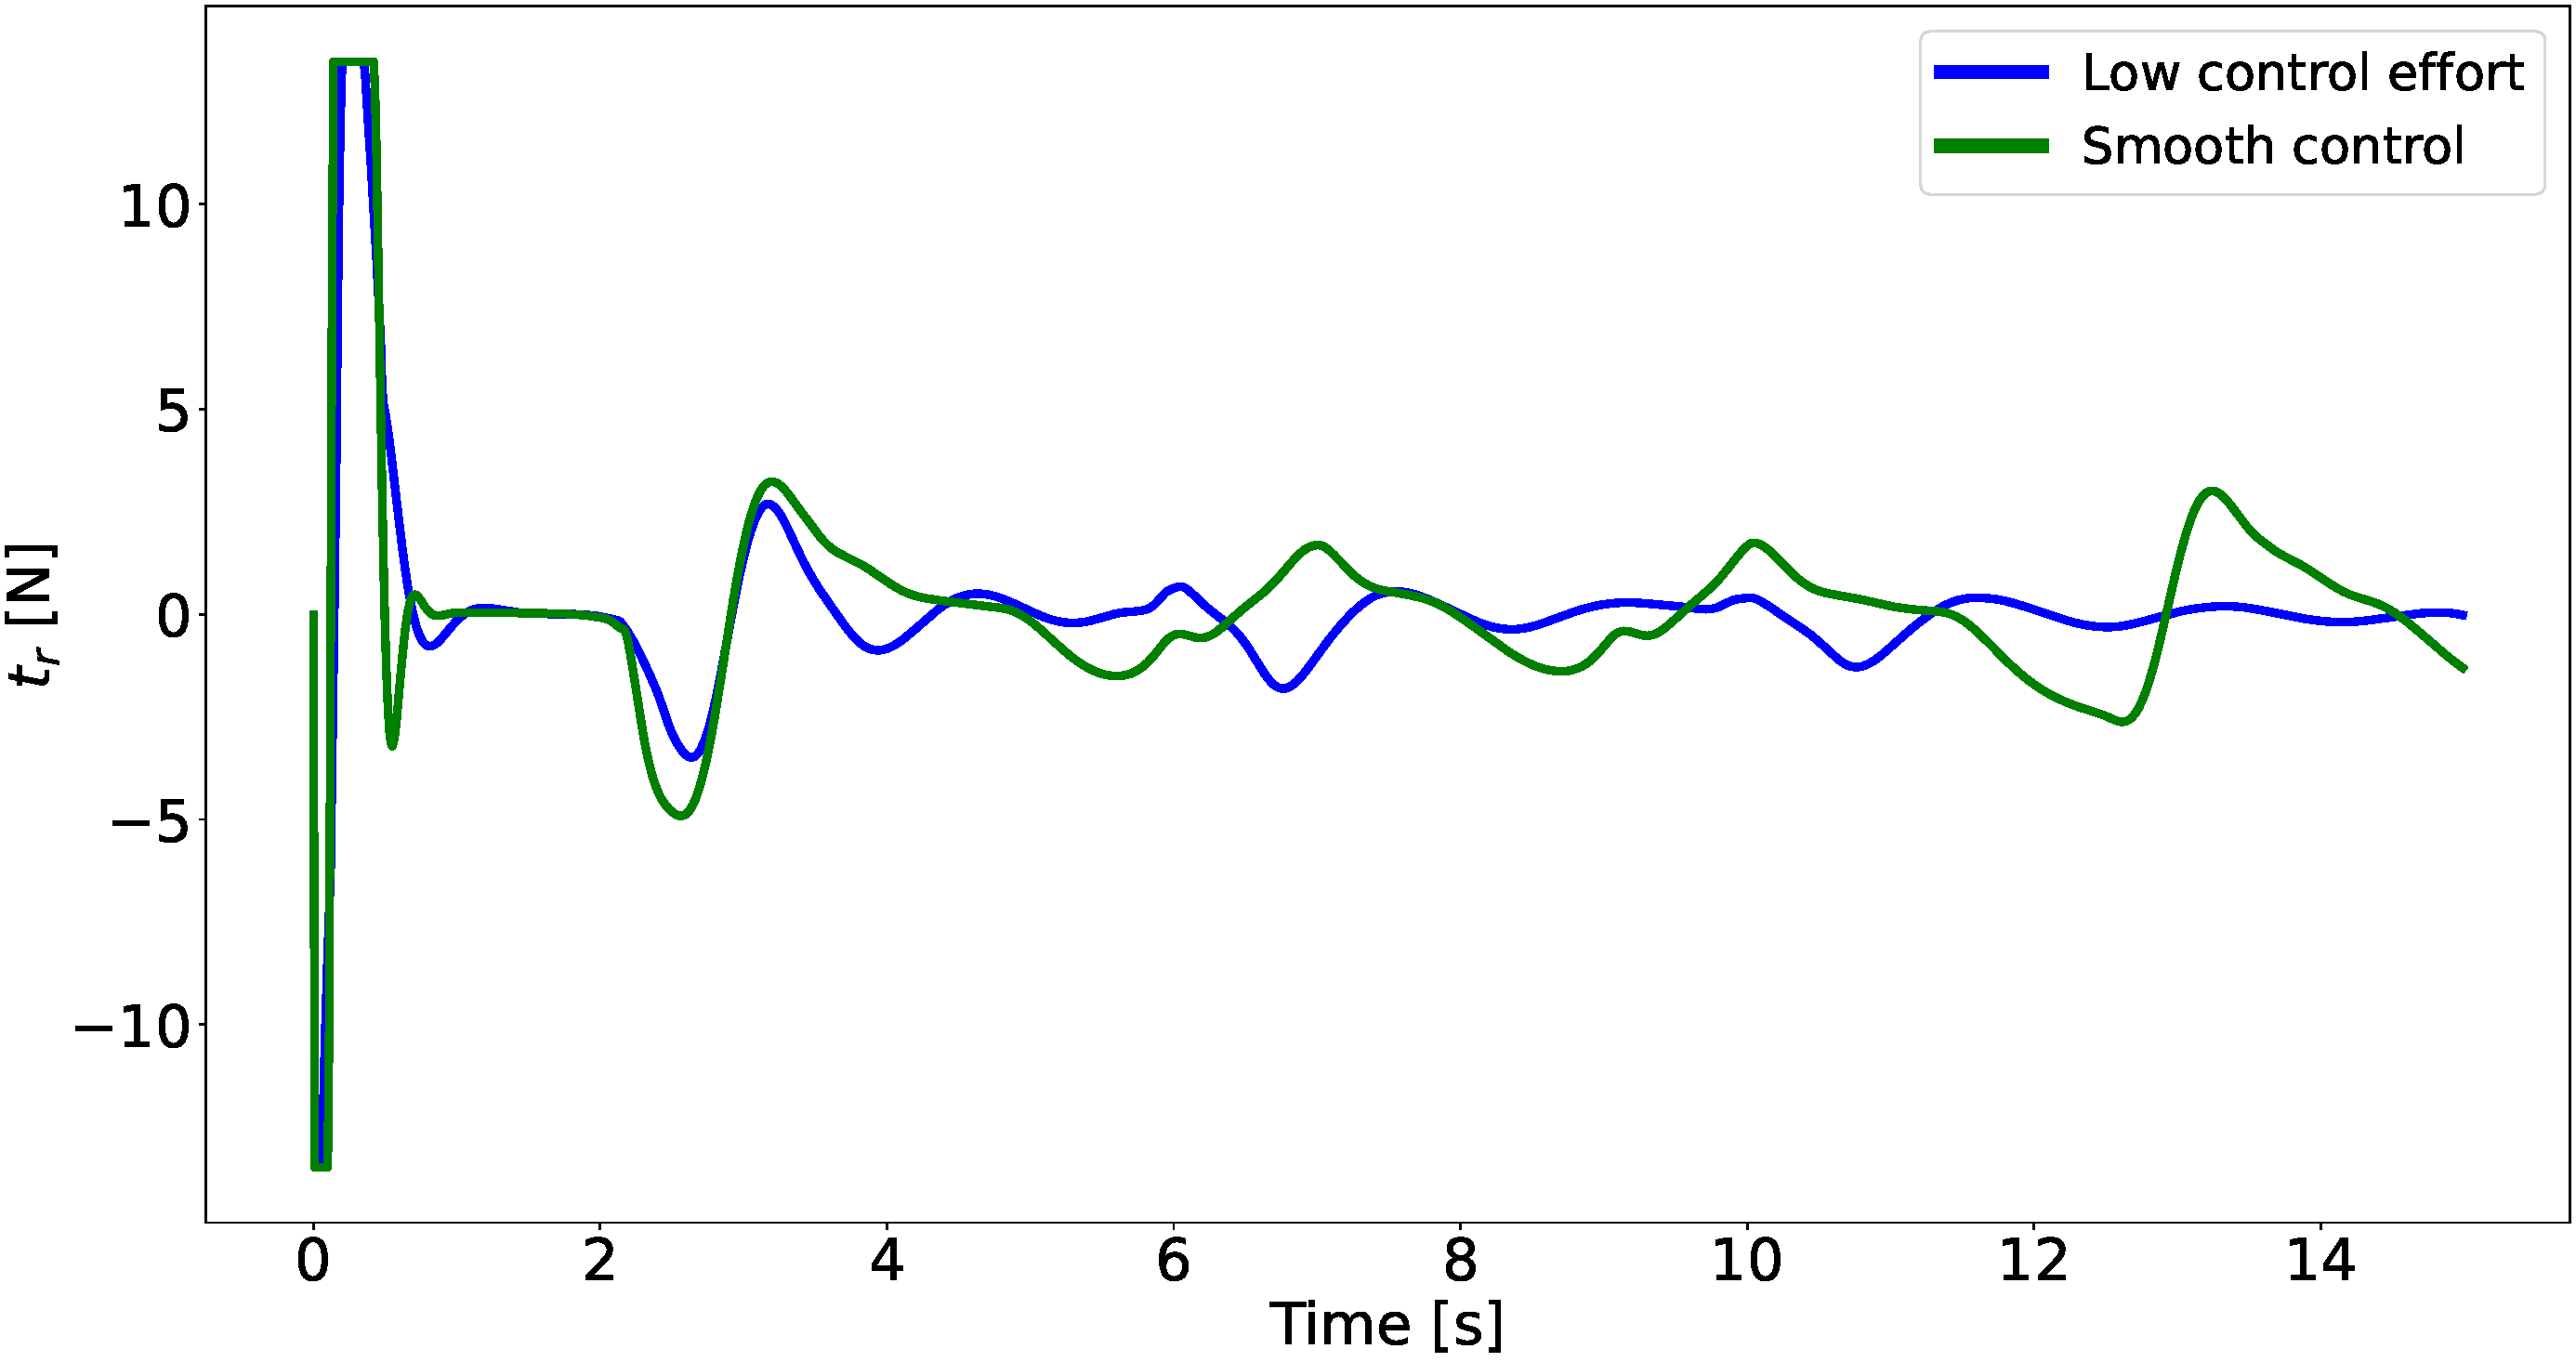
\includegraphics[width=0.48\textwidth]{Figures/One stage OCP/Solver specs comparison/Weights/Virtual speed controlled inside OCP/Planar_onestage_ocp_control_vspeed_comp_tr_limited_weights.pdf}
        \label{subfig:PathTrackCompWeightsVarInsideVspeed_tr}
	}
	\hspace{-1.0em}
    \subfigure[Controlled virtual speed outside \acrshort{nmpc}]{
        \centering
        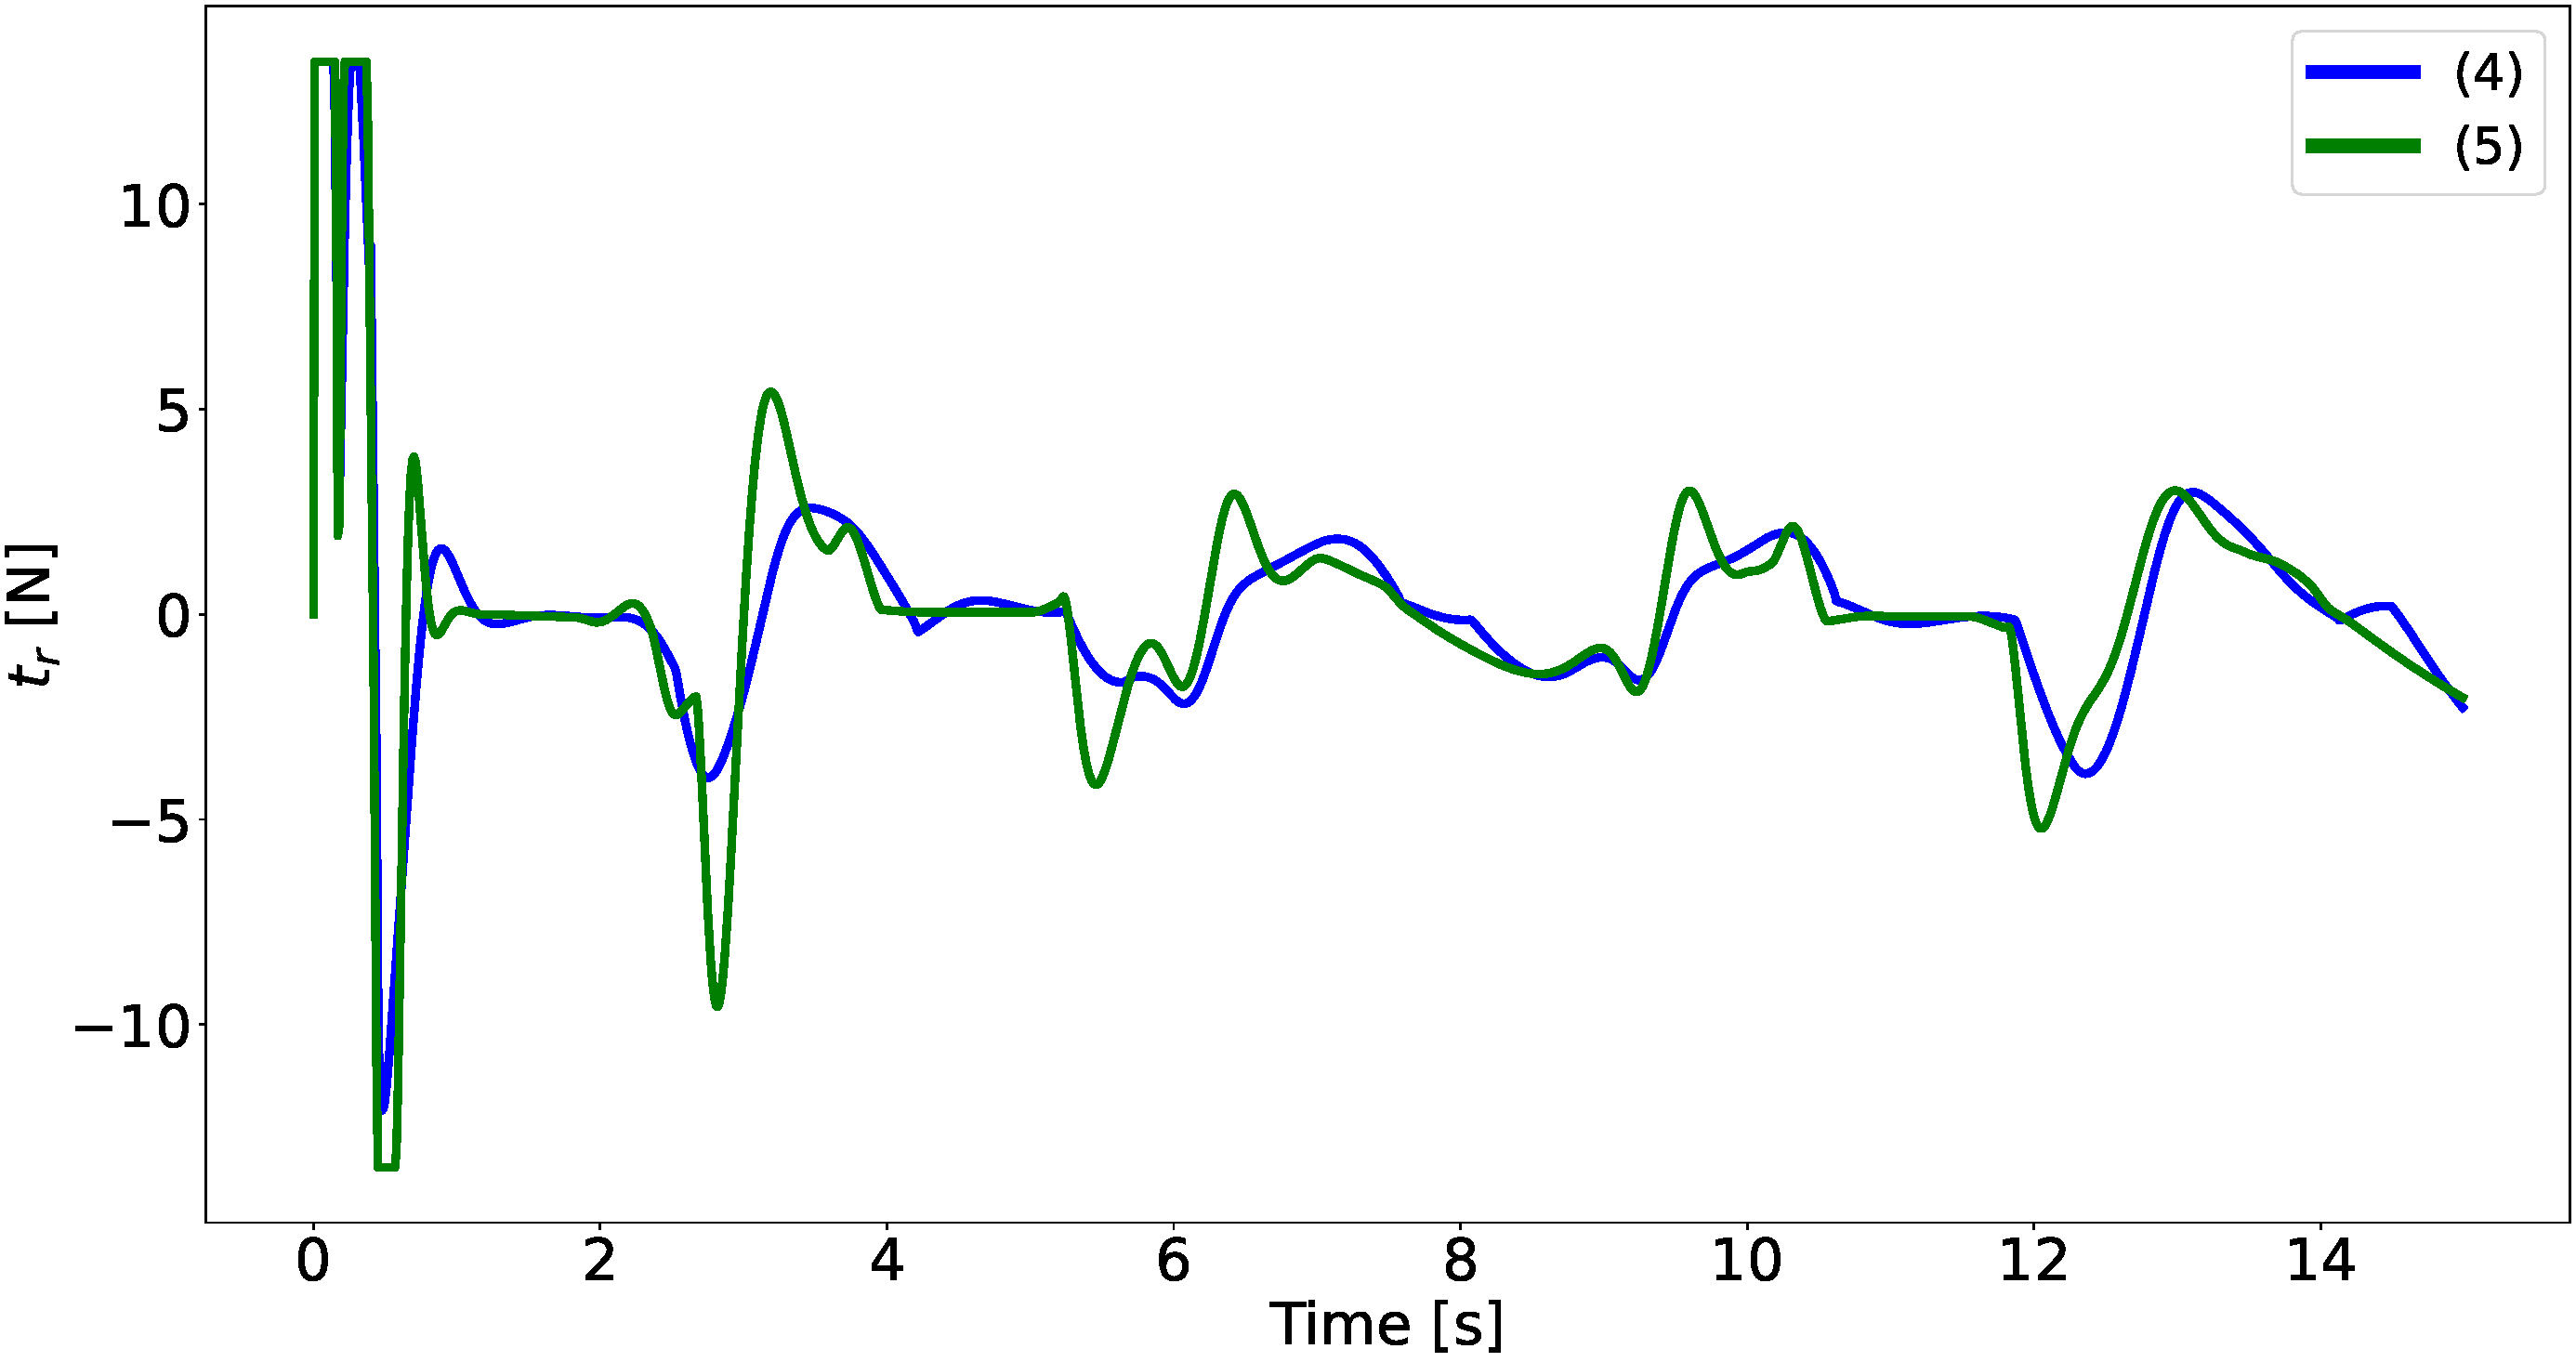
\includegraphics[width=0.48\textwidth]{Figures/One stage OCP/Solver specs comparison/Weights/Virtual speed controlled outside OCP/Planar_onestage_ocp_control_outside_vspeed_comp_tr_limited_weights.pdf}
        \label{subfig:PathTrackCompWeightsVarOutsideVspeed_tr}
	}
	\caption{$\Traction_r$ curve comparison between controllers \textit{Low control effort} and \textit{Smooth control}.}
	\label{fig:PathTrackCompWeightsVar_tr_limited}
\end{figure}

For the most part, the analysis of tables \ref{tab:cumulativeControlEffortWeights}, \ref{tab:cumulativePositionalErrorWeights} and \ref{tab:cumulativeHeadingErrorWeights} show us that each controller excels on its purpose with respect to other controllers on both architectures. Moreover, a look to figures \ref{fig:PathTrackCompWeightsVar_tl_limited} and \ref{fig:PathTrackCompWeightsVar_tr_limited} shows that $\Traction_l$ and $\Traction_r$ stay closer to zero with respect to other controllers, whereas the same variables present a smoother behaviour under the rule of controller \textit{Smooth control}, although it may reach higher values than controller \textit{Low control effort}. Even though the latter achieves its energy saving goal, it compromises a lot on reference tracking, so some care shall be taken from now on to carefully promote energy saving whenever possible, without compromising on reference tracking.

\begin{remark}
Energy saving may also be achieved with optimal path planning (chapter \ref{chapter:globalpathplanner}) or by reaching a goal state faster. However, limits to its velocities must be set, for the sake of safety.
\end{remark}

\subsubsection*{Subsection summary}

The analysis performed in this subsection has provided a good rule of thumbs to bear in mind. First, a good balance on the control horizon shall be found so that a good trade-off with respect to positional and heading errors is found. Then, the sampling time shall be increased whenever possible, although the solver computation time sets the sampling time's reference.

Finally, each set of cost function weights has achieved its purpose. However, the controller must be set up so that a single and specific control objective is solely pursued. Both architectures follow the same trends, although the virtual speed control inside the \acrshort{nmpc} delivers a better performance.

\subsection{Real-time planar \acrshort{nmpc}}
\label{subsection:realTimeOneStagePlanarOCP}

In this subsection, a similar analysis to the one performed previously is carried on for an \acrshort{nmpc} implemented in \texttt{acados}. This time, virtual speed will only be controlled outside the \acrshort{nmpc}. A real-time \acrshort{nmpc} must meet stringent time requirements, which may make it unfeasible to handle considerable non-convexities and non-linearities. So, as the problem of path planning may be solved outside the solver, the virtual speed control is managed outside the \acrshort{nmpc}. The closest point computation is always performed, when applicable. Once again, a small reformulation of the cost function is performed in \refeq{eq:realtimeplanarocpcost}.
\begin{subequations}
	\begin{align}
		\lagrangeTerm{\mathbf{\x},\,\mathbf{u},\,\mathbf{p}}_k = \Vert\x - r_{\x},\,&\y - r_{\y},\,e_{\yaw},\,v_{x},\,\omega_{z},\,\Traction_{l},\,\Traction_{r}\Vert_{Q,\,k}^2 + \Vert u_{l},\,u_{r} \Vert_{R,\,k}^2 \label{subeq:realtimeonestagelagrange}\\
		\mayerTerm{\mathbf{\x},\,\mathbf{p}}_k &= \Vert \x - r_{\x},\,\y - r_{\y},\,e_{\yaw},\,v_{x},\,\omega_{z},\,\Traction_{l},\,\Traction_{r} \Vert_{Q,\,k}^2 \label{subeq:realtimeonestagemayer}
	\end{align}
	\label{eq:realtimeplanarocpcost}
\end{subequations}

In this analysis, the optimization time is also considered. \acrshort{sqprti} is selected as solver. Due to that, assumptions from \ref{assumption:rti1} to \ref{assumption:rti5} shall be taken into account in order to yield a global optimal solution. An exact hessian is computed and partial-condensing \texttt{\acrshort{hpipm}} is selected as the \acrshort{qp} solver.

\subsubsection*{Regulation problem}

The \acrshort{nmpc} is tested in a position and heading regulation scenarios. The results are presented in figures \ref{fig:PositionRegulationCompRealTimeOCP} and \ref{fig:HeadingRegulationCompRealTimeOCP}, respectively. Table \ref{tab:regulatorWeights} denotes the set of weights and parameters for each type of controller. The Coulomb friction constraint is enforced as well.

\begin{table}[!htb]
  \caption{Regulator solver parameters. Controllers $^p$ and $^h$ are used for position and heading regulation, respectively.}
  \label{tab:regulatorWeights}
  \renewcommand{\arraystretch}{1.1}
  \centering
  \begin{tabular}[]{lcccccc}
	\toprule
    Type of controller & $Q$ & $R$\\
	\midrule
    Baseline & $diag\left(1.0,\,1.0,\,1.0,\,1\mathrm{e}{-9},\,1\mathrm{e}{-9},\,1\mathrm{e}{-9},\,1\mathrm{e}{-9}\right)$ & $1\mathrm{e}{-3}\cdot \mathbf{1}_2$\\
	Standard$^p$ & $diag\left(1.0,\,1.0,\,1.0,\,1\mathrm{e}{-9},\,1\mathrm{e}{-9},\,1\mathrm{e}{-9},\,1\mathrm{e}{-9}\right)$ & $1\mathrm{e}{-9}\cdot \mathbf{1}_2$\\
	Position regulator$^p$ & $diag\left(3.0,\,3.0,\,1.0,\,1\mathrm{e}{-9},\,1\mathrm{e}{-9},\,1\mathrm{e}{-9},\,1\mathrm{e}{-9}\right)$ & $1\mathrm{e}{-9}\cdot \mathbf{1}_2$\\
	Low control effort$^p$ & $diag\left(3.0,\,3.0,\,1.0,\,1\mathrm{e}{-9},\,1\mathrm{e}{-9},\,1\mathrm{e}{-6},\,1\mathrm{e}{-6}\right)$ & $1\mathrm{e}{-3}\cdot \mathbf{1}_2$\\
	Smooth controls$^p$ & $diag\left(3.0,\,3.0,\,1.0,\,1\mathrm{e}{-9},\,1\mathrm{e}{-9},\,1\mathrm{e}{-9},\,1\mathrm{e}{-9}\right)$ & $1\mathrm{e}{-3}\cdot \mathbf{1}_2$\\
	Standard$^h$ & $diag\left(1.0,\,1.0,\,1.0,\,1\mathrm{e}{-9},\,1\mathrm{e}{-9},\,1\mathrm{e}{-9},\,1\mathrm{e}{-9}\right)$ & $1\mathrm{e}{-9}\cdot \mathbf{1}_2$\\
	Heading regulator$^h$ & $diag\left(1.0,\,1.0,\,3.0,\,1\mathrm{e}{-9},\,1\mathrm{e}{-9},\,1\mathrm{e}{-9},\,1\mathrm{e}{-9}\right)$ & $1\mathrm{e}{-9}\cdot \mathbf{1}_2$\\
	Low control effort$^h$ & $diag\left(1.0,\,1.0,\,3.0,\,1\mathrm{e}{-9},\,1\mathrm{e}{-9},\,1\mathrm{e}{-6},\,1\mathrm{e}{-6}\right)$ & $1\mathrm{e}{-3}\cdot \mathbf{1}_2$\\
	Smooth controls$^h$ & $diag\left(1.0,\,1.0,\,3.0,\,1\mathrm{e}{-9},\,1\mathrm{e}{-9},\,1\mathrm{e}{-9},\,1\mathrm{e}{-9}\right)$ & $1\mathrm{e}{-3}\cdot \mathbf{1}_2$\\
  	\toprule
  	$\left[(v_x)_{min},\; (v_x)_{max}\right]\,[m/s]$ & $\left[(\omega_z)_{min},\; (\omega_z)_{max}\right]\,[rad/s]$ & $\left[u_{i,\,min},\,u_{i,\,max}\right]\,[N \cdot s]$ & $\FrictionCoefficient$\\
  	\midrule
  	$\left[-0.5,\,0.5\right]$ & $\left[-100,\,100\right]$ & $\left[-1000,\,1000\right]$ & $1.0$\\
  	\bottomrule
  \end{tabular}
\end{table}

\begin{figure}[!htb]
	\centering
	\subfigure[$T_s = 10\,ms\;\&\;$Baseline]{
        \centering
        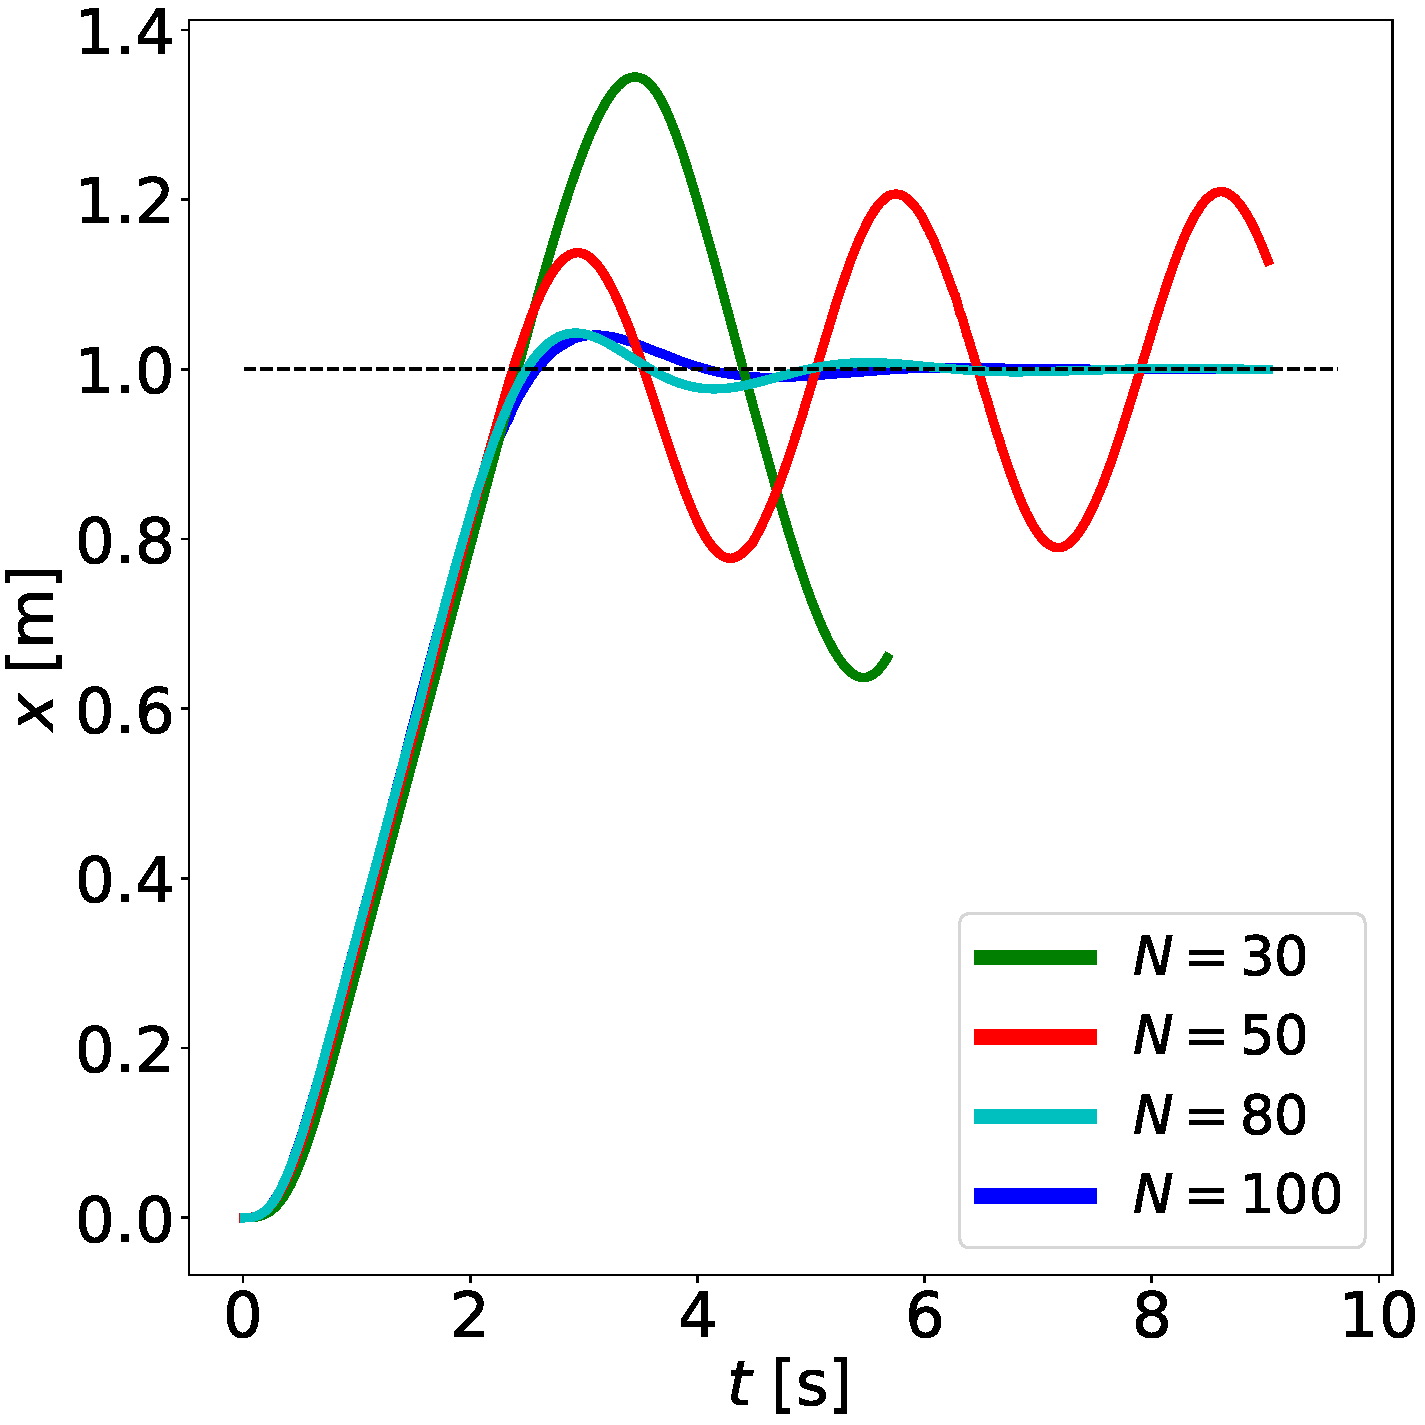
\includegraphics[width=0.315\textwidth]{Figures/Real time one stage planar OCP/Regulation/Position_regulation_horizon.pdf}
        \label{subfig:PositionRegulationCompHorizonRealTimeOCP}
	}
	\hspace{-1.0em}
    \subfigure[$N = 100\;\&\;$Baseline]{
        \centering
        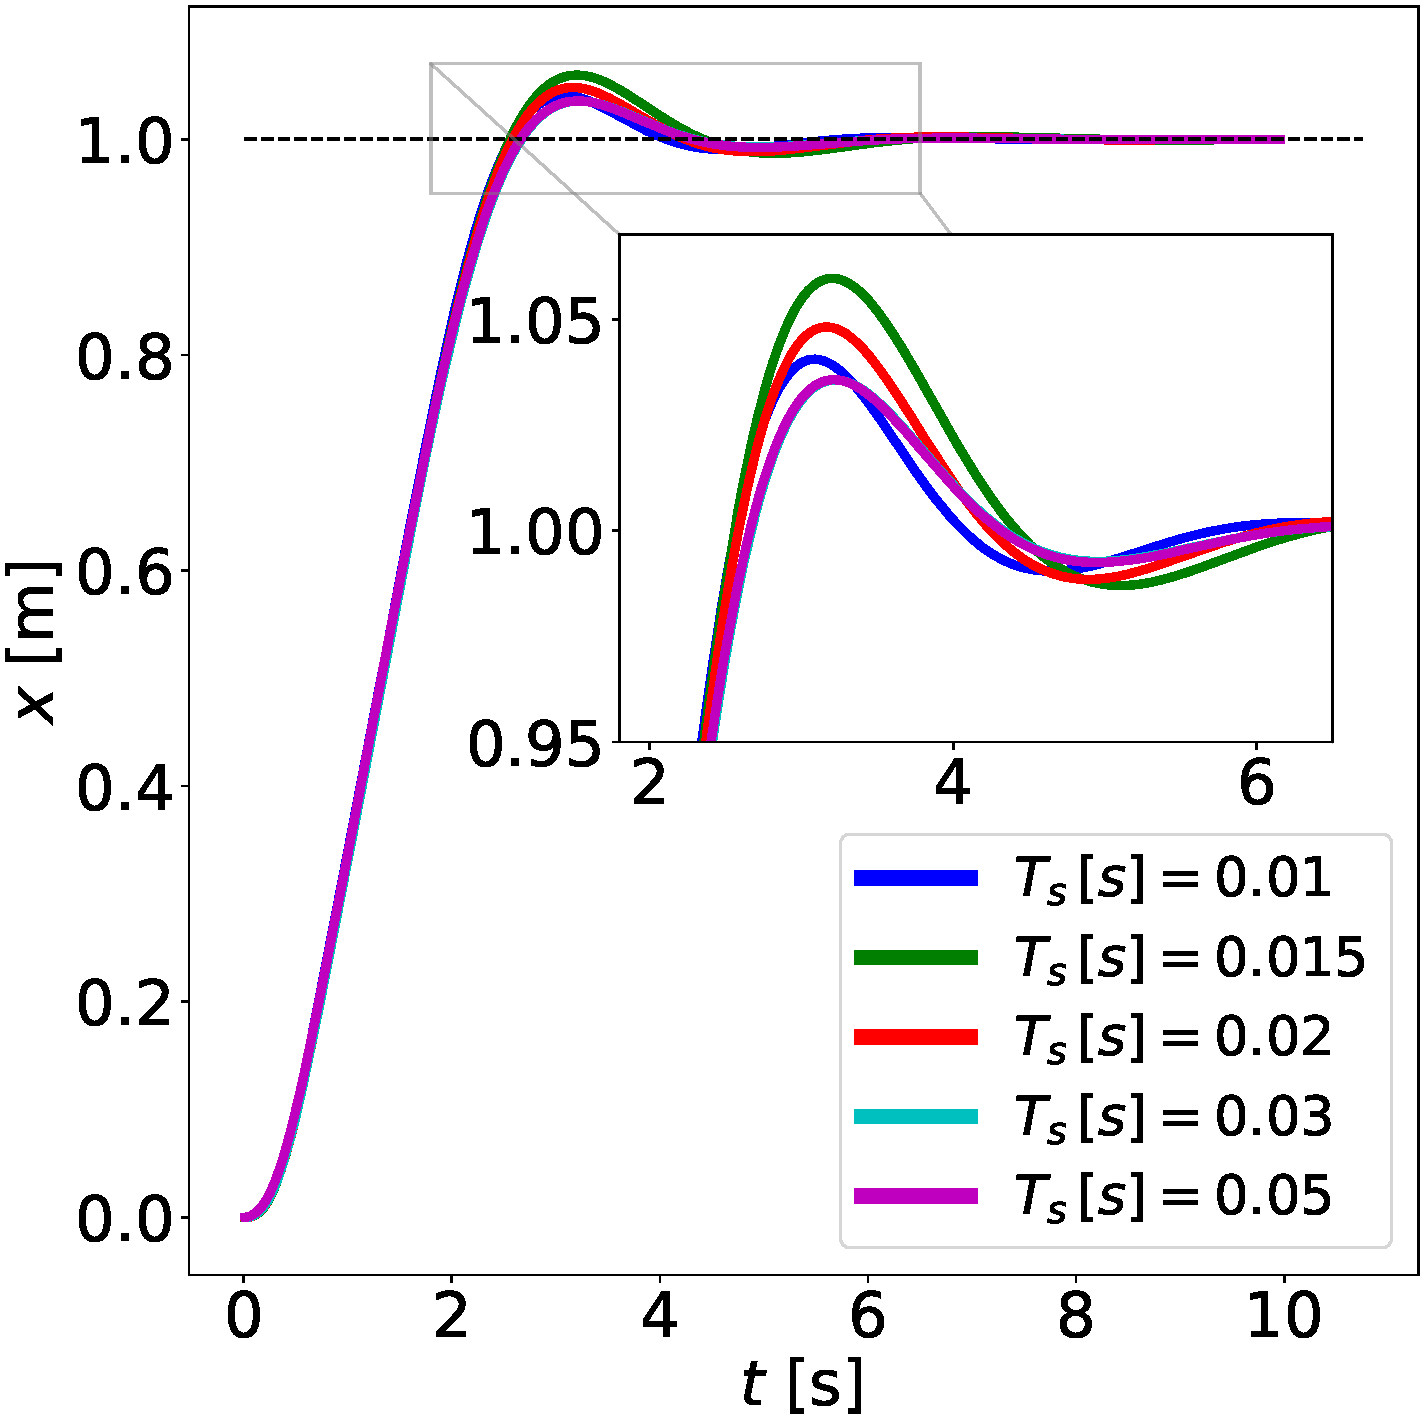
\includegraphics[width=0.315\textwidth]{Figures/Real time one stage planar OCP/Regulation/Position_regulation_sampling_time.pdf}
        \label{subfig:PositionRegulationCompTimeRealTimeOCP}
	}
	\subfigure[$T_s = 30\,ms\;\&\;N=100$]{
        \centering
        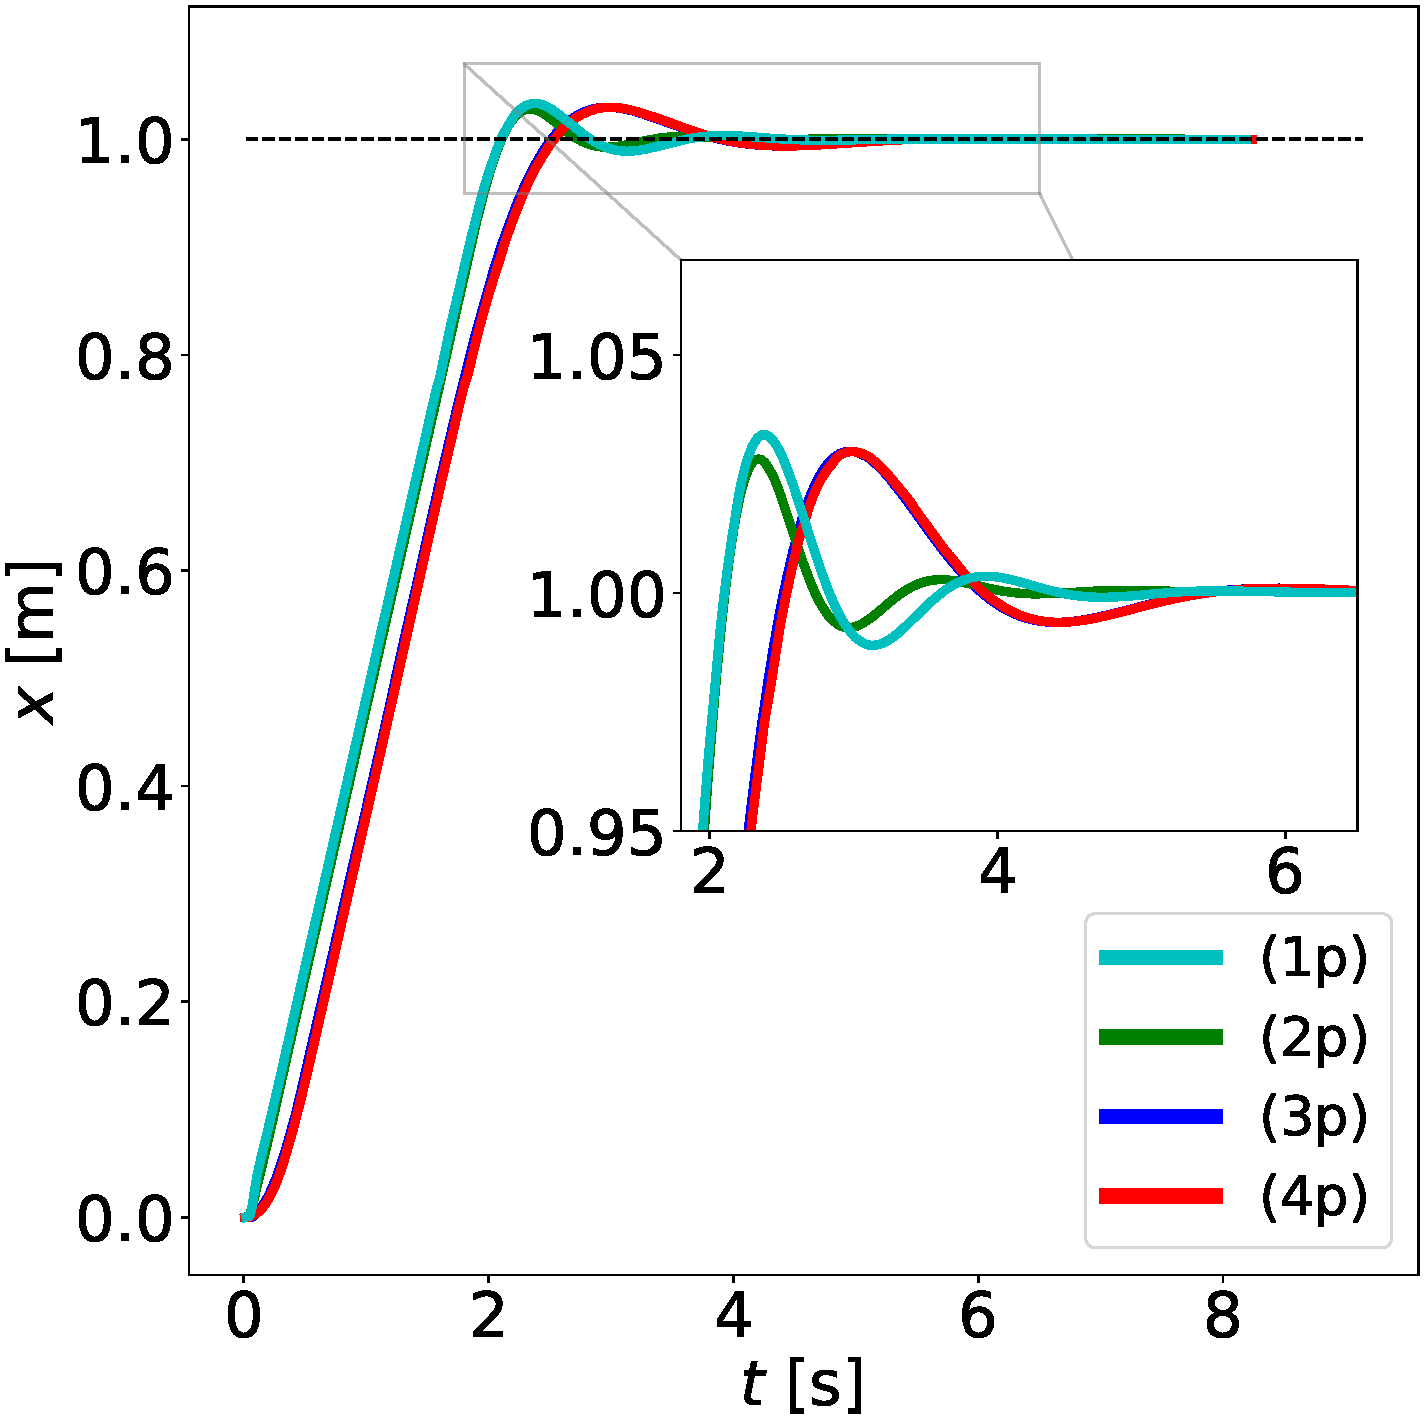
\includegraphics[width=0.315\textwidth]{Figures/Real time one stage planar OCP/Regulation/Position_regulation_weights.pdf}
        \label{subfig:PositionRegulationCompWeightsRealTimeOCP}
	}
	\caption{Comparison among position regulations.}
	\label{fig:PositionRegulationCompRealTimeOCP}
\end{figure}

\begin{figure}[!htb]
	\centering
	\subfigure[$T_s = 10\,ms\;\&\;$Baseline]{
        \centering
        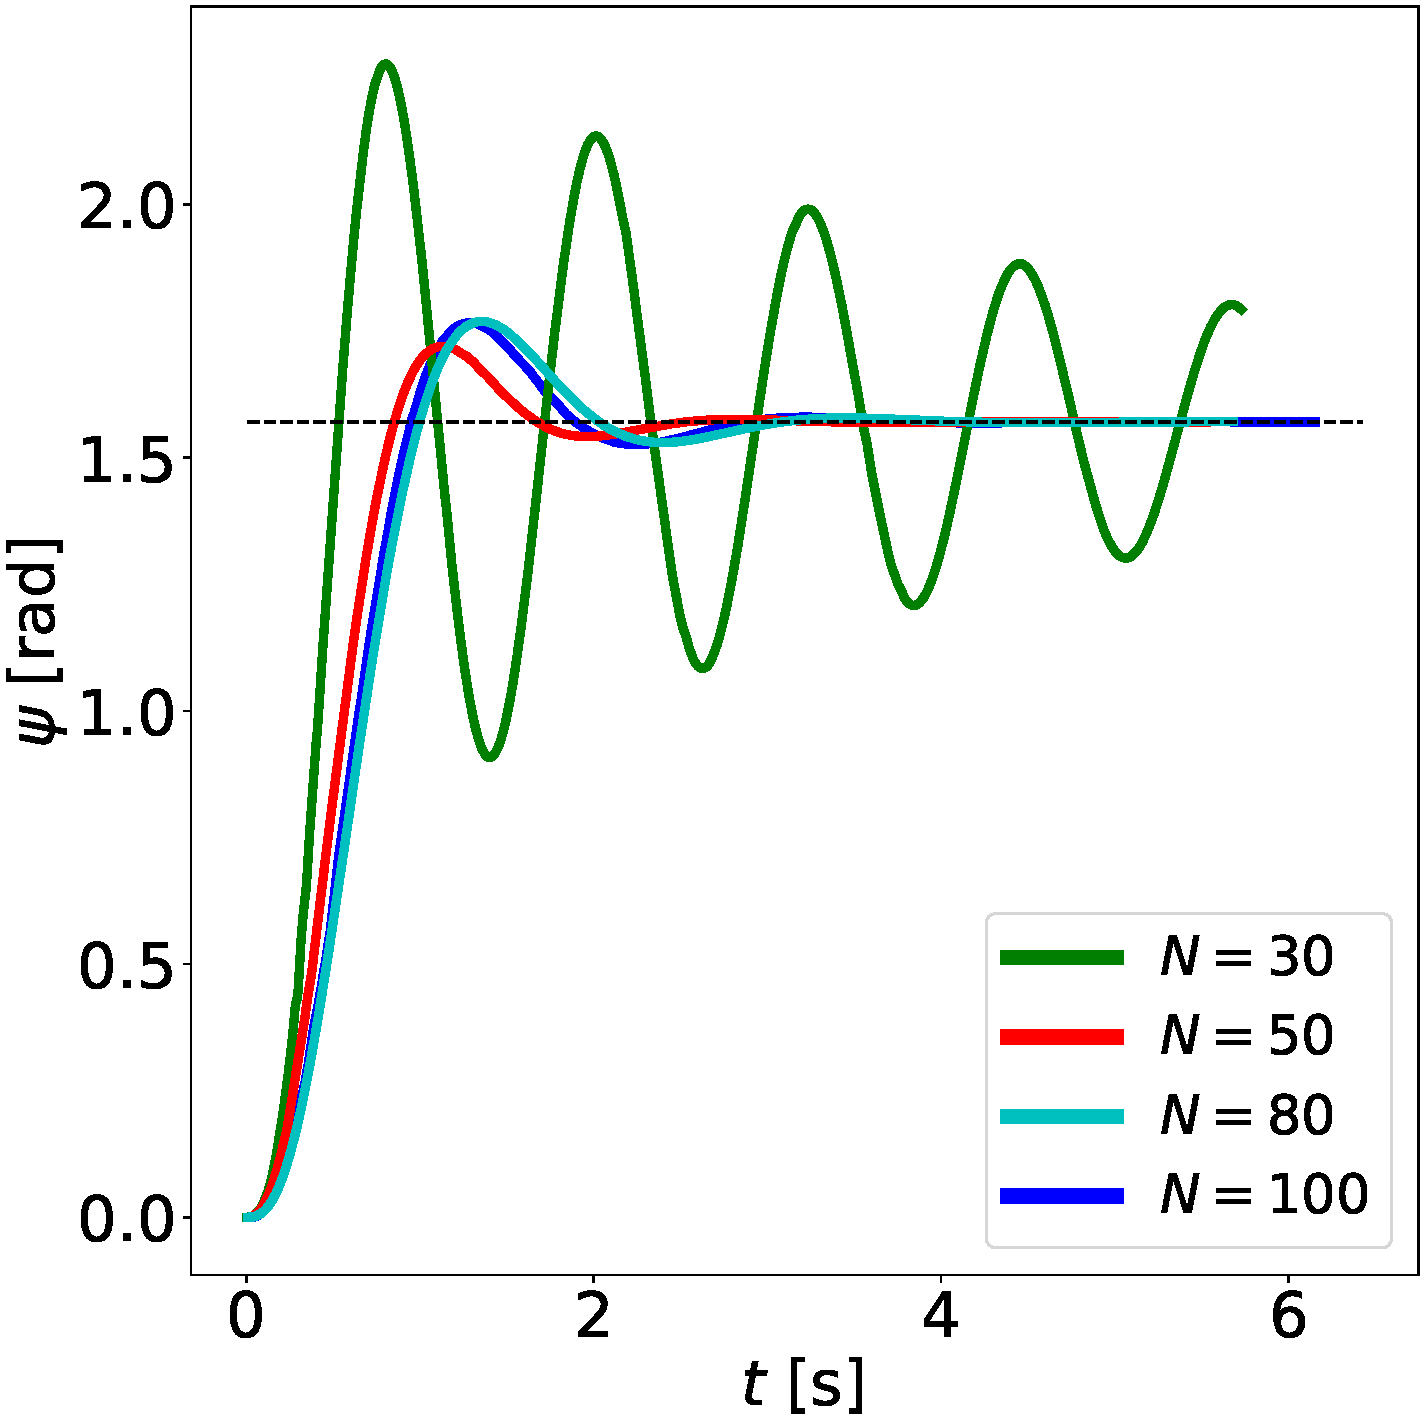
\includegraphics[width=0.315\textwidth]{Figures/Real time one stage planar OCP/Regulation/Heading_regulation_horizon.pdf}
        \label{subfig:HeadingRegulationCompHorizonRealTimeOCP}
	}
	\hspace{-1.0em}
    \subfigure[$N = 100\;\&\;$Baseline]{
        \centering
        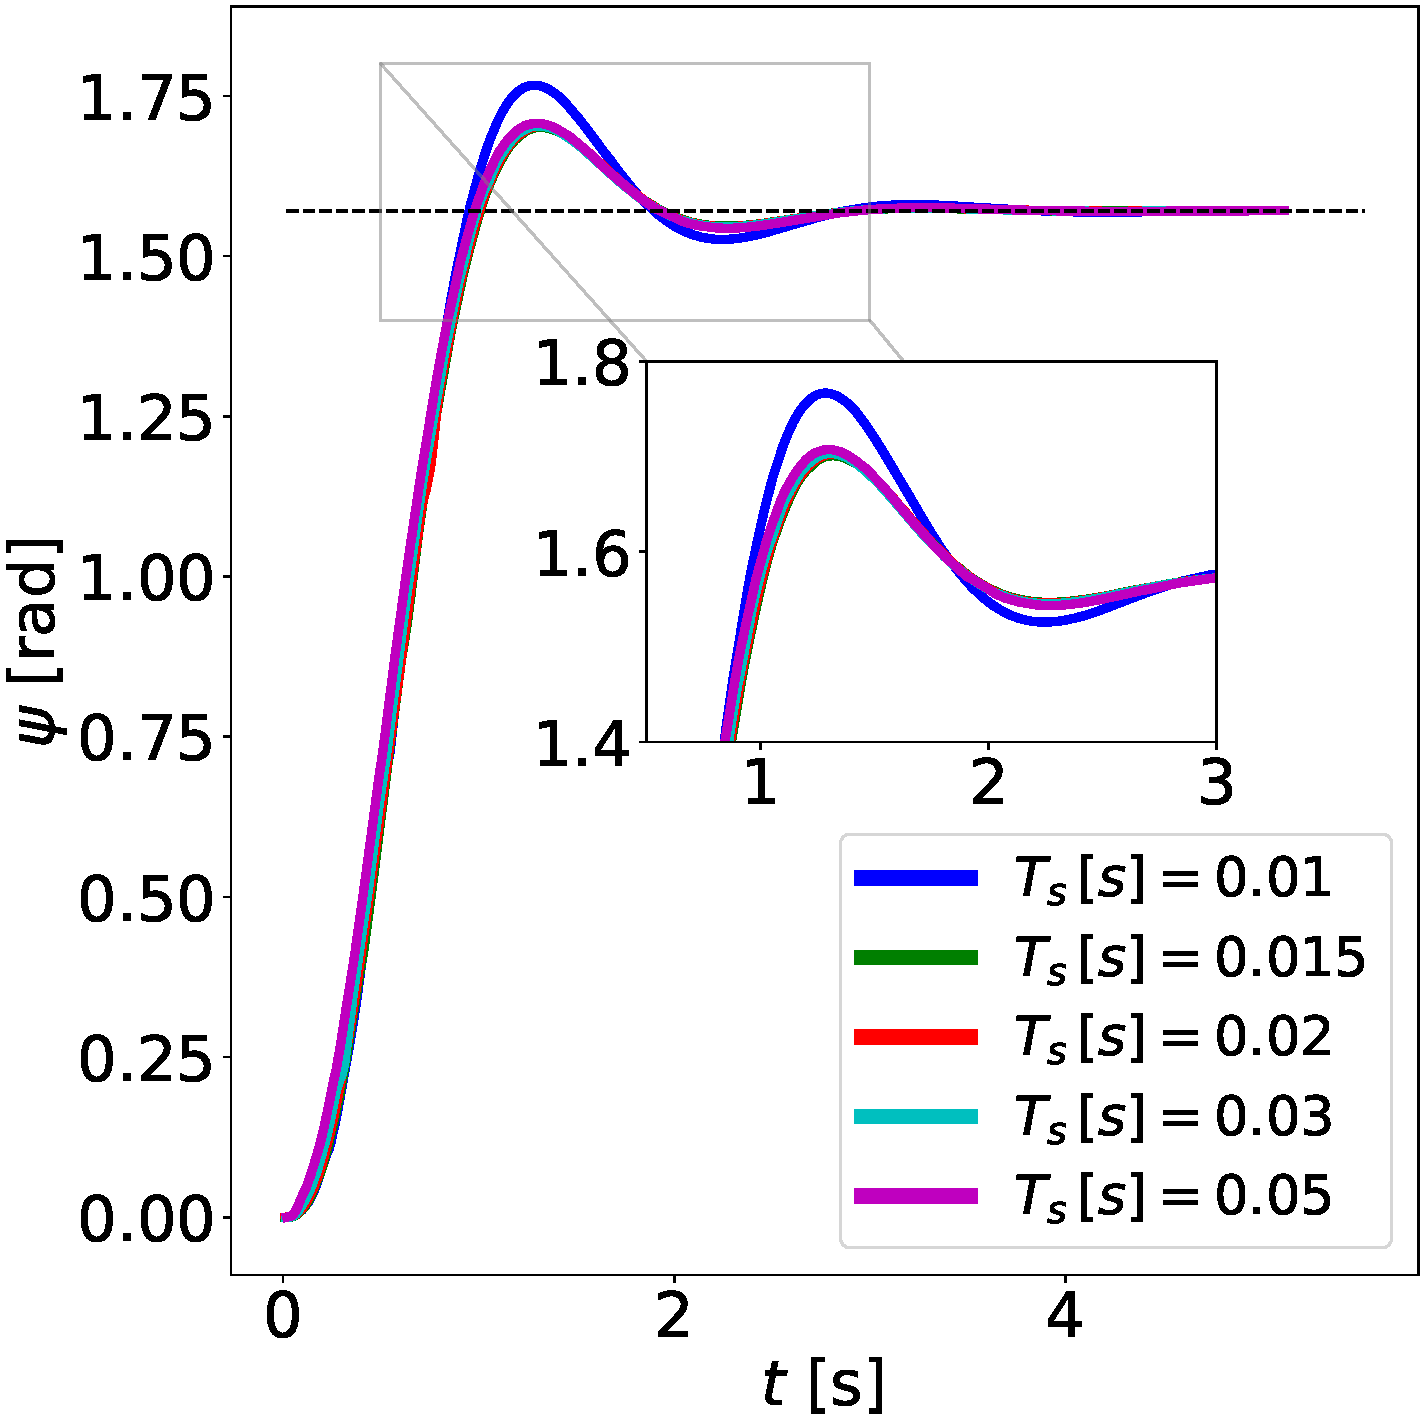
\includegraphics[width=0.315\textwidth]{Figures/Real time one stage planar OCP/Regulation/Heading_regulation_sampling_time.pdf}
        \label{subfig:HeadingRegulationCompTimeRealTimeOCP}
	}
	\subfigure[$T_s = 30\,ms\;\&\;N=100$]{
        \centering
        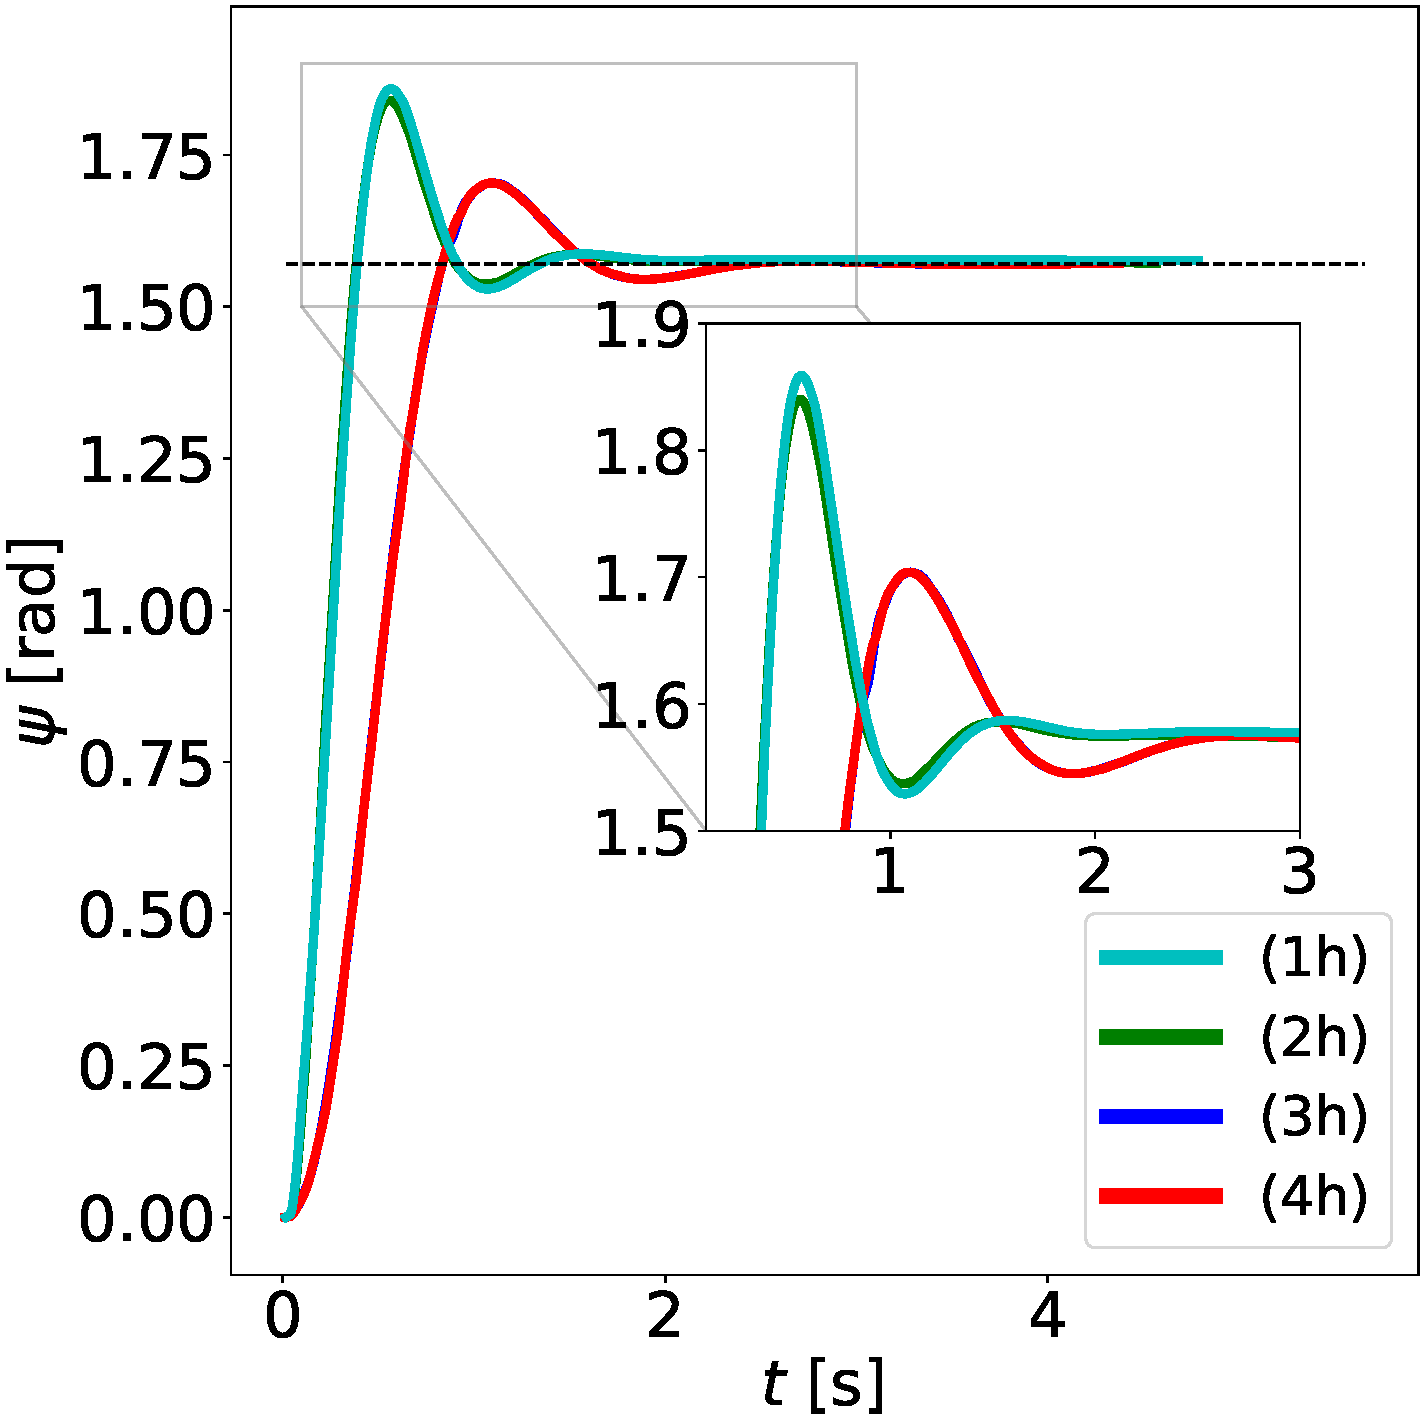
\includegraphics[width=0.315\textwidth]{Figures/Real time one stage planar OCP/Regulation/Heading_regulation_weights.pdf}
        \label{subfig:HeadingRegulationCompWeightsRealTimeOCP}
	}
	\caption{Comparison among heading regulations.}
	\label{fig:HeadingRegulationCompRealTimeOCP}
\end{figure}

In both scenarios, it is clear that a higher time horizon correlates well with low overshoot and fast settling times. When it comes to a comparison among the type of controllers, a higher weight on the reference and on the controls rate of change yields a more stable regulation, with less ups and downs. In all simulations, the computation time is below the sampling time and the optimal cost approaches zero in case the regulation is performed effectively.

\subsubsection*{Path tracking problem}

Up to now, it is possible to address the path tracking problem, as the results of regulation and subsection \ref{subsection:solverspecssurvey} provide a good rule of thumbs. At the end, comprehensive results of the best solvers are presented.

\begin{figure}[h]
    \centering
    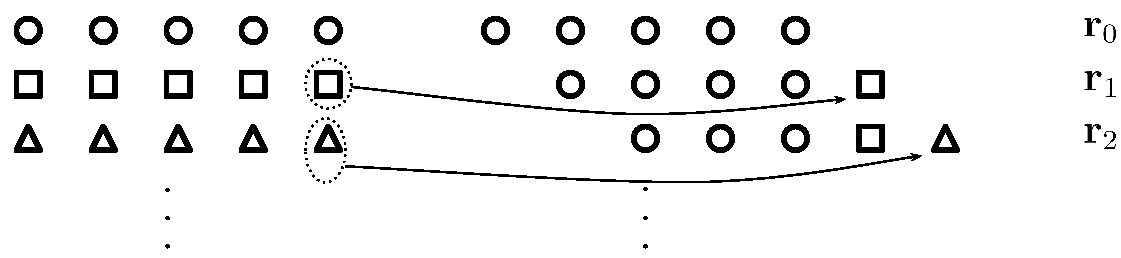
\includegraphics[width=0.8\textwidth]{Figures/reference_switch.pdf}
    \caption{Reference shift between consecutive iterations. In every iteration, a full reference is computed as in the standard case. However, the reference that is fed into the \acrshort{nmpc} is shifted by removing the first node and appending the last node of the standard reference to it. This variant of the reference generation was tested because it offers a greater compliance with assumption \ref{assumption:rti3}.}
    \label{fig:refswitch}
\end{figure}

The solver is tested under several conditions, which are outlined in table \ref{tab:pathTrackingSpecs}. In figure \ref{fig:pathtrackingperformance}, the performance metrics of the solvers are presented. The reference provided to the \acrshort{nmpc} is updated on every node, by taking the nearest point to the trajectory as the first reference node. When $\dagger$ is appended to the controller number, that means the reference provided to the solver is updated incrementally (figure \ref{fig:refswitch}), where the reference horizon is shifted forward and a new reference pose is added to the last node \cite{gros2020linear}. Moreover, the optimization cost (time) is determined as the sum of the preparation and feedback phase costs (times) (see algorithm \nameref{alg:rti}).

Up to now, the virtual speed control module was just made of \refeq{eq:vspeed_computation_architecture_b}. From now on, a weighted average of \refeq{eq:virtualspeedqp} follows it, in order to promote smooth reference changes. A scheme of the virtual speed control module reformulation is presented in figure \ref{fig:virtual_speed_module_qp}.

\begin{figure}[!htb]
  \begin{minipage}[c]{0.60\linewidth}
    \centering
    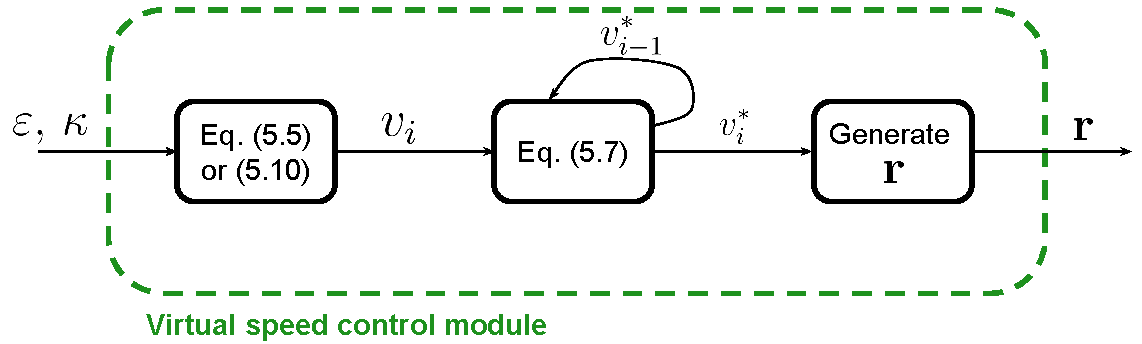
\includegraphics[width=\linewidth]{Figures/Real time one stage planar OCP/Path tracking/Virtual_speed_control_module.pdf}
  \end{minipage}
  \begin{minipage}[c]{0.35\linewidth}
    \centering
    \begin{equation}
		v_i^* = 0.3 \cdot v_i + 0.7 \cdot v^*_{i-1}
		\label{eq:virtualspeedqp}
	\end{equation}
  \end{minipage}
\caption{Detail view of virtual speed control module and weighted average equation.}
\label{fig:virtual_speed_module_qp}
\end{figure}

On every controller, the loop time is below the sampling time. The loop times of controllers $(i^{\dagger})$ are lower because the \acrshort{nmpc} changes minimally from iteration to iteration. However, controllers $i$ present a lower optimization cost, due to the fact that these controllers don't match the pose horizon with the reference. The cost of controllers $(i^{\dagger})$ is higher because the reference does not take into account the change of pose between consecutive iterations. Then, controllers $(i)$ are a better choice because their cost is very low, even though the computational time is higher, but still well below the sampling time.

Moreover, lower loop times are recorded when variable weights are used, as the states horizon is more stable \cite{schoels2020nmpc}. In the case of constant weights, an oscillatory behaviour of the solution between iterations is recorded.

\begin{table}[!htb]
  \caption[Planar path tracking solver parameters ($N = 50,\; T_s = 20\,ms$). Controllers $^i$ have cost terms with \textit{increasing} weights.]{Planar path tracking solver parameters ($N = 50,\; T_s = 20\,ms$). Controllers $^i$ have cost terms with \textit{increasing} weights.}
  \label{tab:pathTrackingSpecs}
  \renewcommand{\arraystretch}{1.1}
  \centering
  \begin{tabular}[]{lcc}
	\toprule
	Controller & $Q_i$ & $R$\\
	\midrule
	(1) Pose tracker & $diag\left(3.0 \cdot \mathbf{1}_3,\,1\mathrm{e}{-9} \cdot \mathbf{1}_4\right)$ & $1\mathrm{e}{-3}\cdot \mathbf{1}_2$\\
	(2) Pose tracker$^i$ & $diag\left(3.0 \times 1.1^i \cdot \mathbf{1}_3,\,1\mathrm{e}{-9} \cdot \mathbf{1}_4\right)$ & $1\mathrm{e}{-3}\cdot \mathbf{1}_2$\\
	(3) Energy saver & $diag\left(3.0 \cdot \mathbf{1}_3,\,1\mathrm{e}{-9}\cdot\mathbf{1}_2,\,1\mathrm{e}{-6}\cdot\mathbf{1}_2\right)$ & $1\mathrm{e}{-3}\cdot\mathbf{1}_2$\\
	(4) Energy saver$^i$ & $diag\left(3.0\times 1.1^i \cdot \mathbf{1}_3,\,1\mathrm{e}{-9} \cdot \mathbf{1}_2,\,1\mathrm{e}{-6}\cdot\mathbf{1}_2\right)$ & $1\mathrm{e}{-3}\cdot \mathbf{1}_2$\\
	\end{tabular}
	\begin{tabular}[]{cccccc}
  	\toprule
  		$\left[(v_x)_{min},\; (v_x)_{max}\right]\,[m/s]$ & $\left[(\omega_z)_{min},\; (\omega_z)_{max}\right]\,[rad/s]$ & $\left[u_{i,\,min},\,u_{i,\,max}\right]\,[N \cdot s]$ & $\FrictionCoefficient$\\
  	\midrule
  		$\left[-5.0,\,5.0\right]$ & $\left[-100,\,100\right]$ & $\left[-1000,\,1000\right]$ & $1.0$\\
  	\bottomrule
  \end{tabular}
\end{table}

\begin{figure}[!htb]
  \begin{subfigmatrix}{2}
    \subfigure[Simulation loop times.]{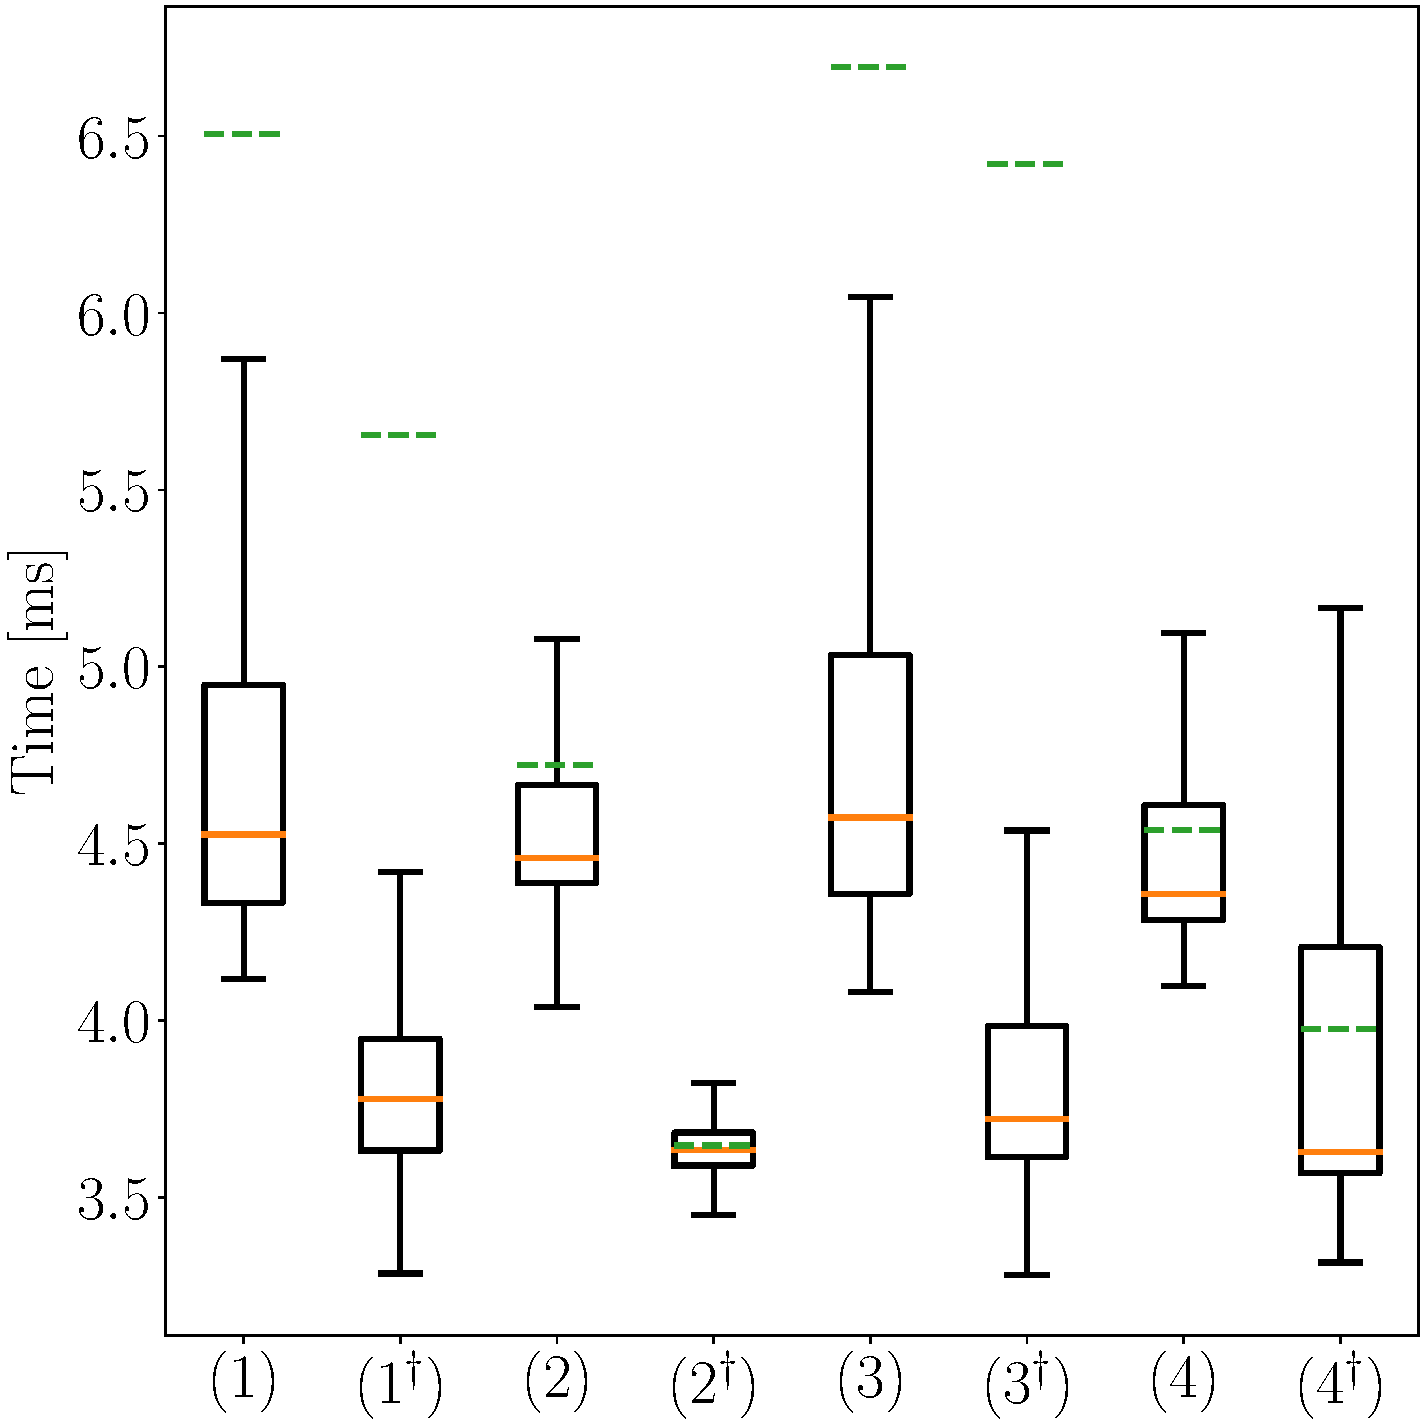
\includegraphics[width=0.49\linewidth]{Figures/Real time one stage planar OCP/Path tracking/cycle times.pdf}}
    \subfigure[Optimization cost.]{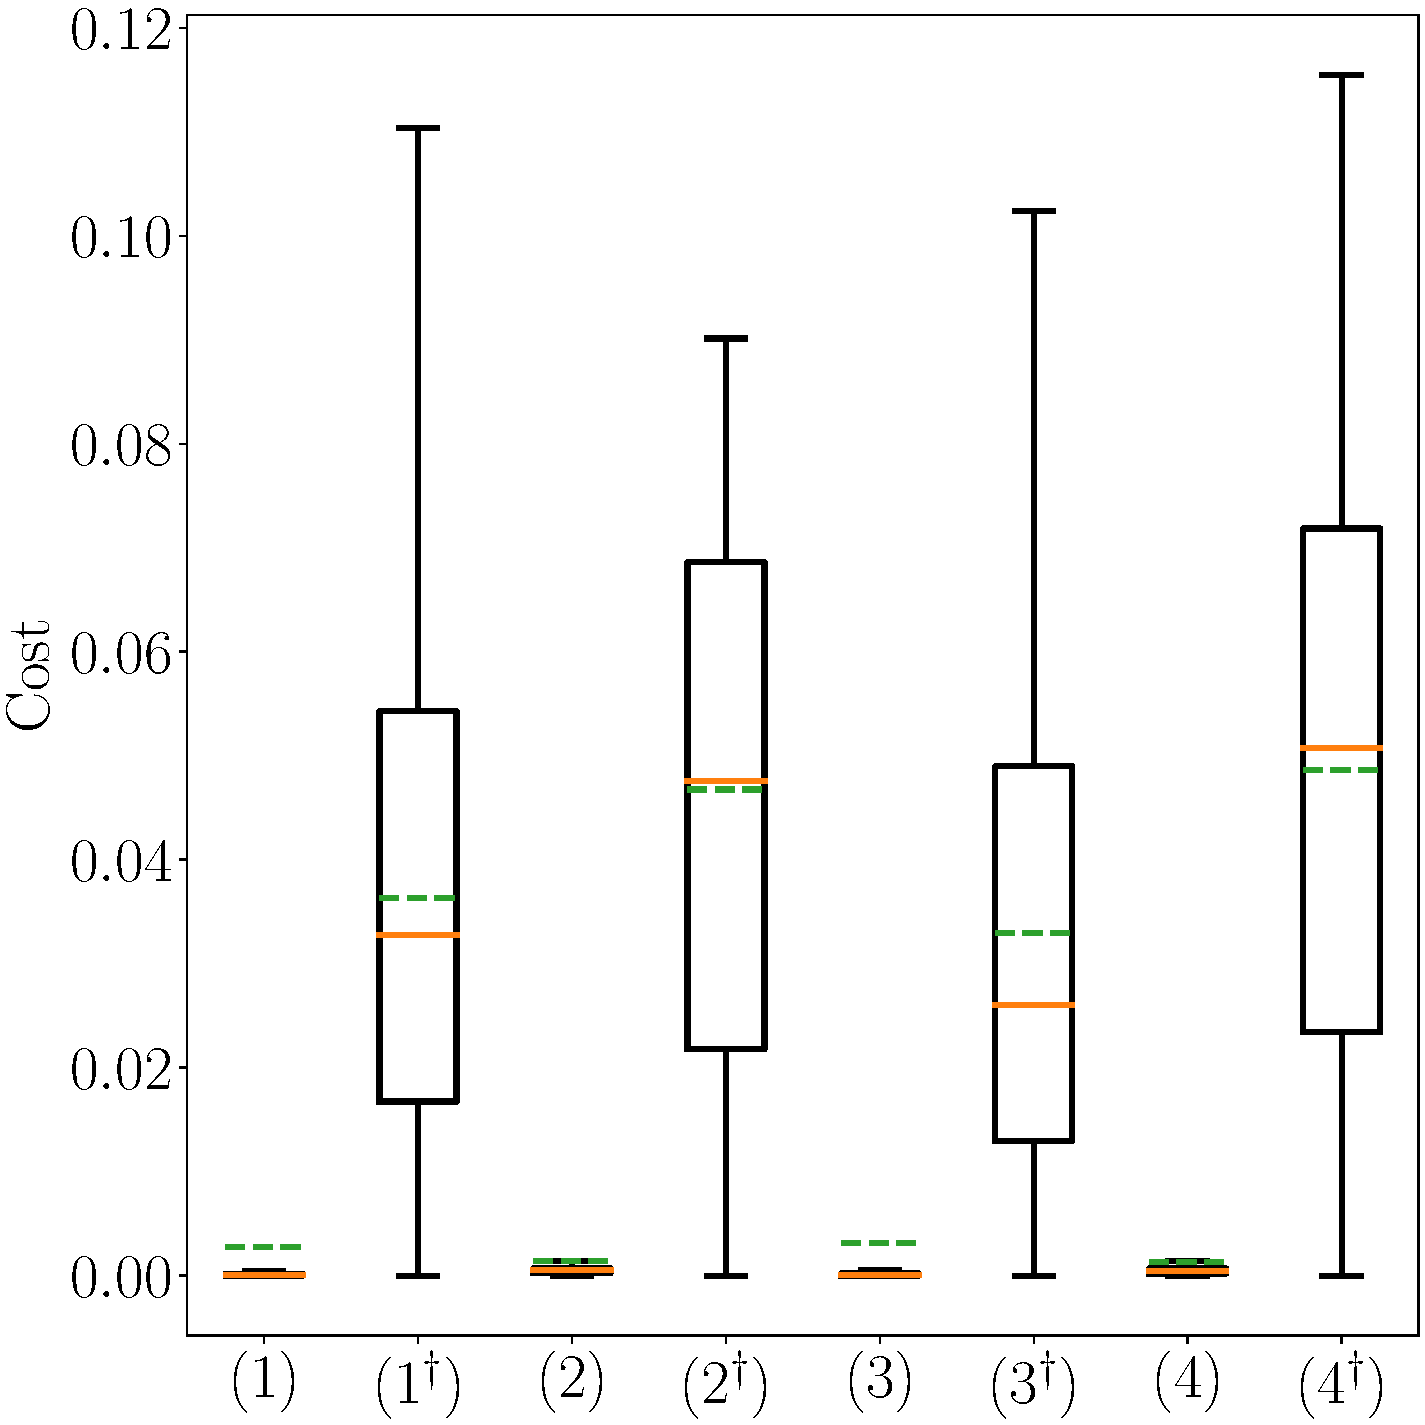
\includegraphics[width=0.49\linewidth]{Figures/Real time one stage planar OCP/Path tracking/optimal_costs.pdf}}
  \end{subfigmatrix}
  \caption{Path tracking performance metrics.}
  \label{fig:pathtrackingperformance}
\end{figure}

It is verified that all solvers effectively track the reference. Figure \ref{subfig:realtimepathtrackingplanarocp} presents the tracking results for the solvers with increasing weights. The solvers not only track the path but also align the vehicle heading so that it does not move backwards. Figure \ref{subfig:energyrealtimepathtrackingplanarocp} also exhibits the correlation between higher cost weights on $\Traction_l$ and $\Traction_r$. However, a higher focus on energy saving delays progress and non-negligible energy saving is only achieved when high penalties are placed on $\Traction_l$ and $\Traction_r$. The results of picture \ref{subfig:energyrealtimepathtrackingplanarocp} were recorded for path tracking simulations with the same reference and initial conditions. From these results and respective analysis, increasing weight controllers will be considered for more complex problems and scenarios.

\begin{figure}[!htb]
  \begin{subfigmatrix}{2}
    \subfigure[Path tracking comparison.]{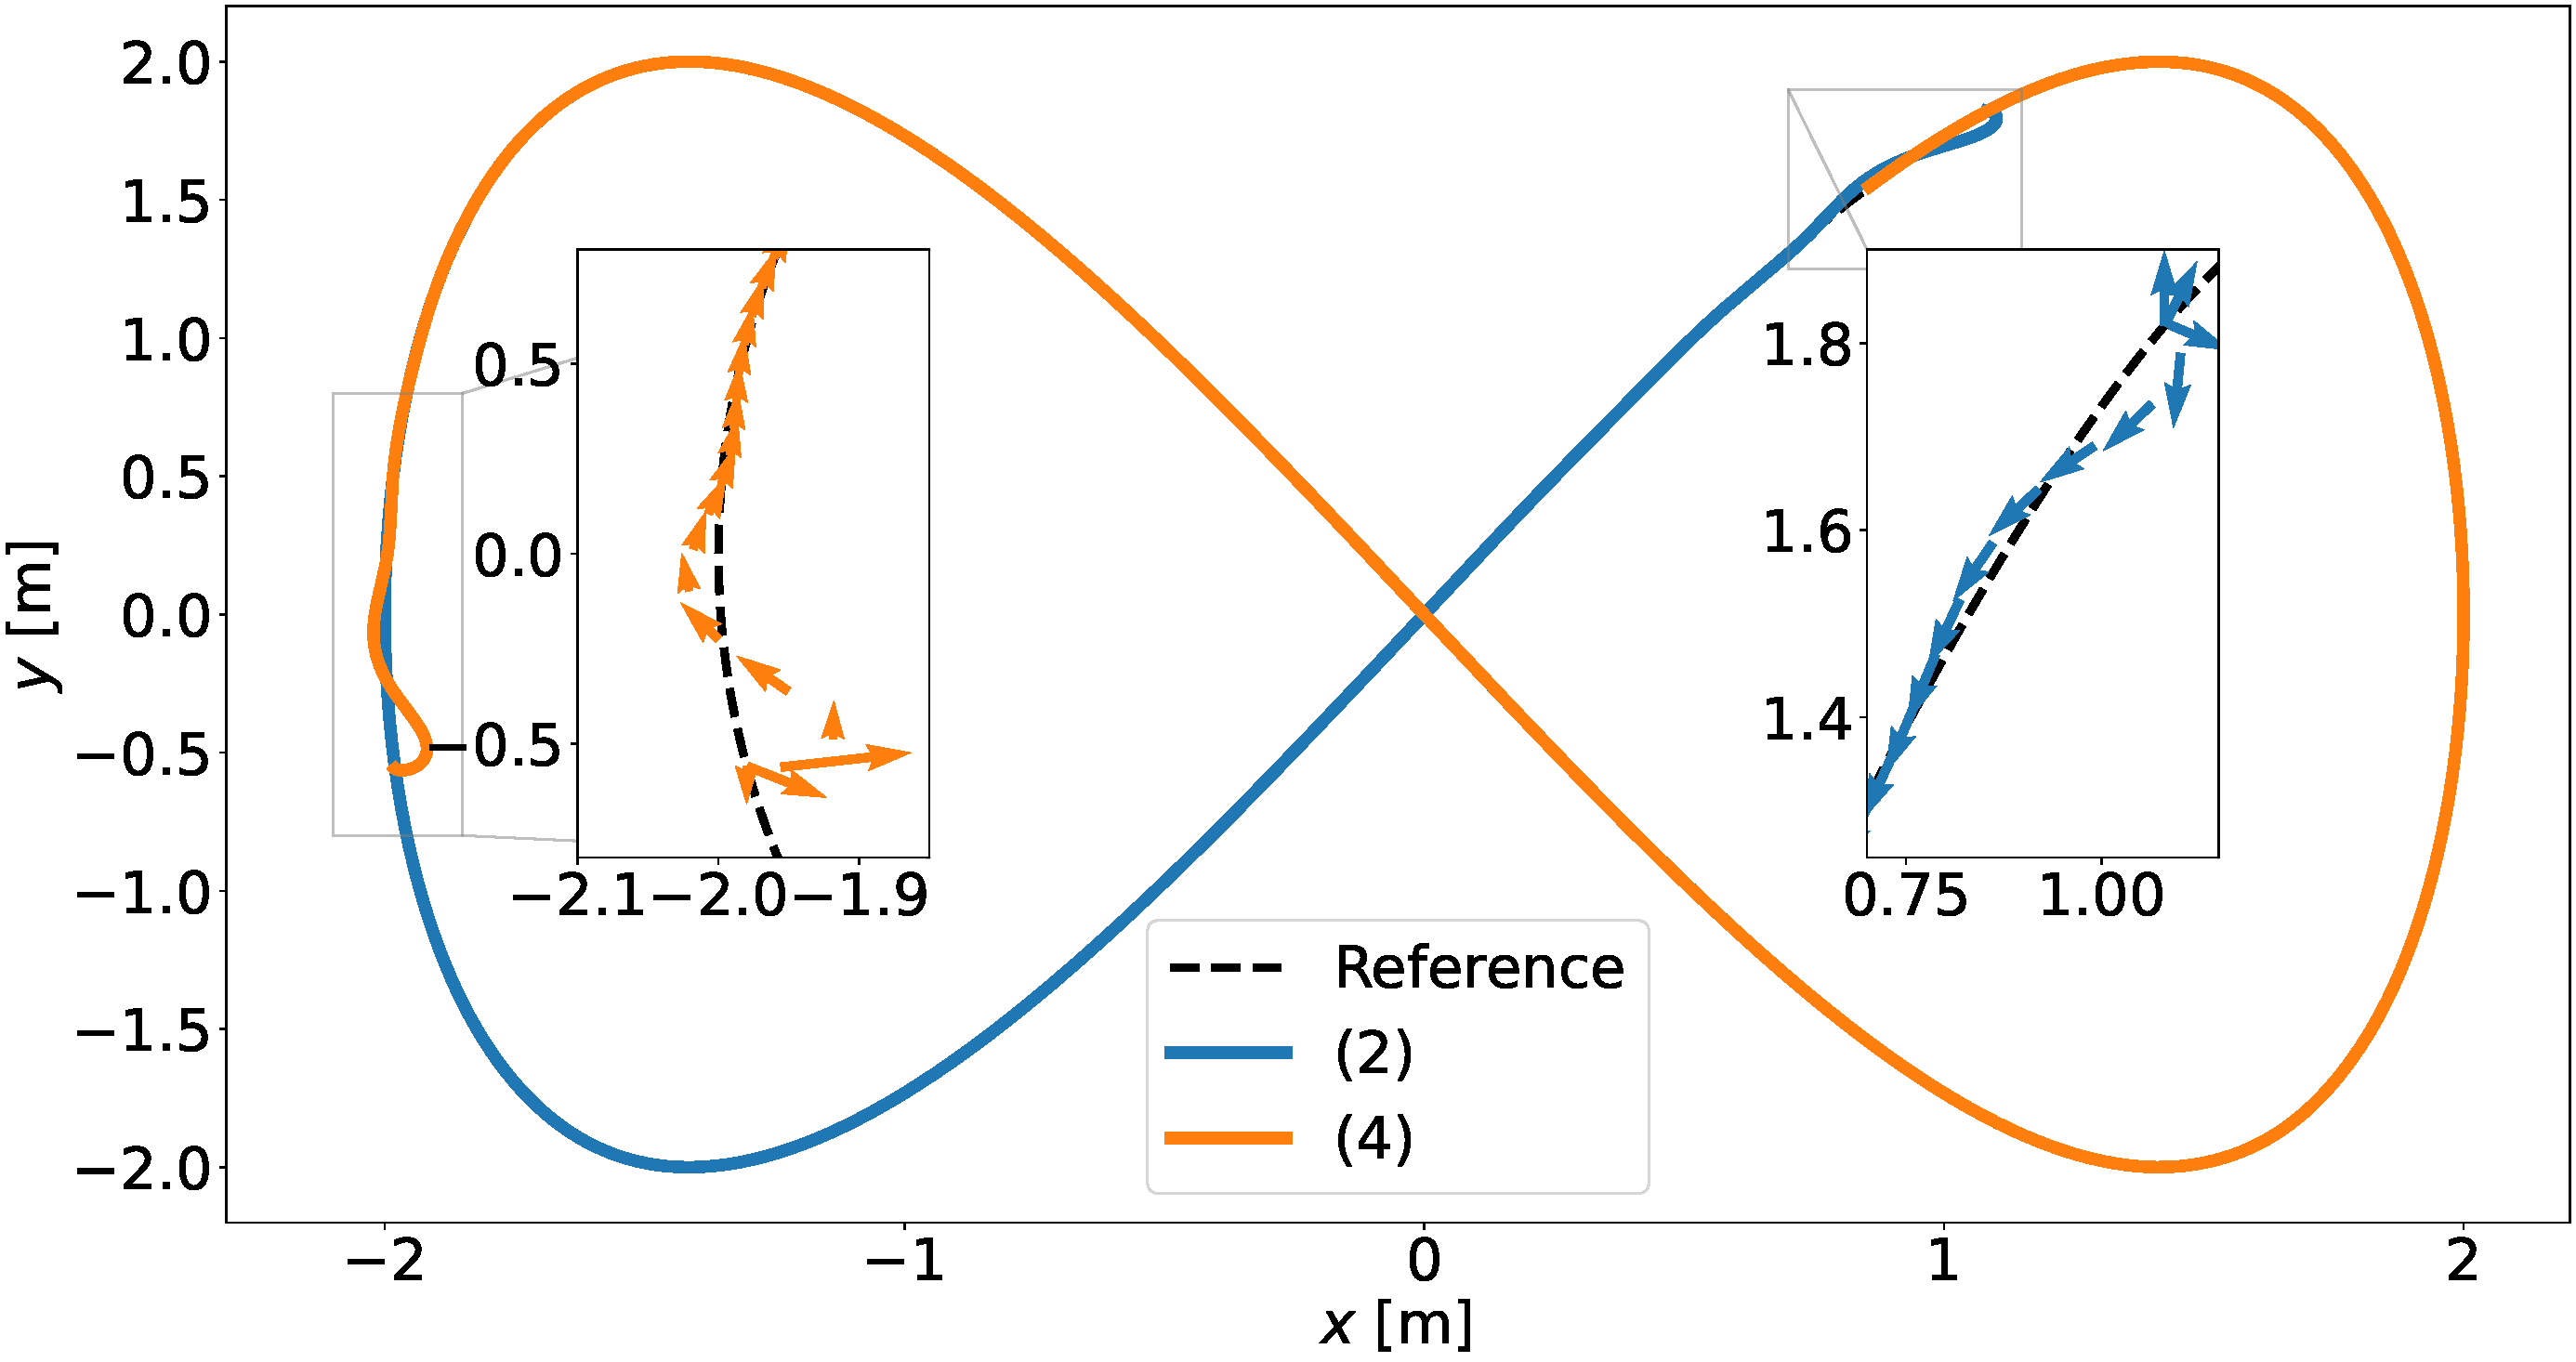
\includegraphics[width=0.49\linewidth]{Figures/Real time one stage planar OCP/Path tracking/path_tracking_comparison.pdf}
    \label{subfig:realtimepathtrackingplanarocp}}
    \subfigure[Cumulative sum of traction forces.]{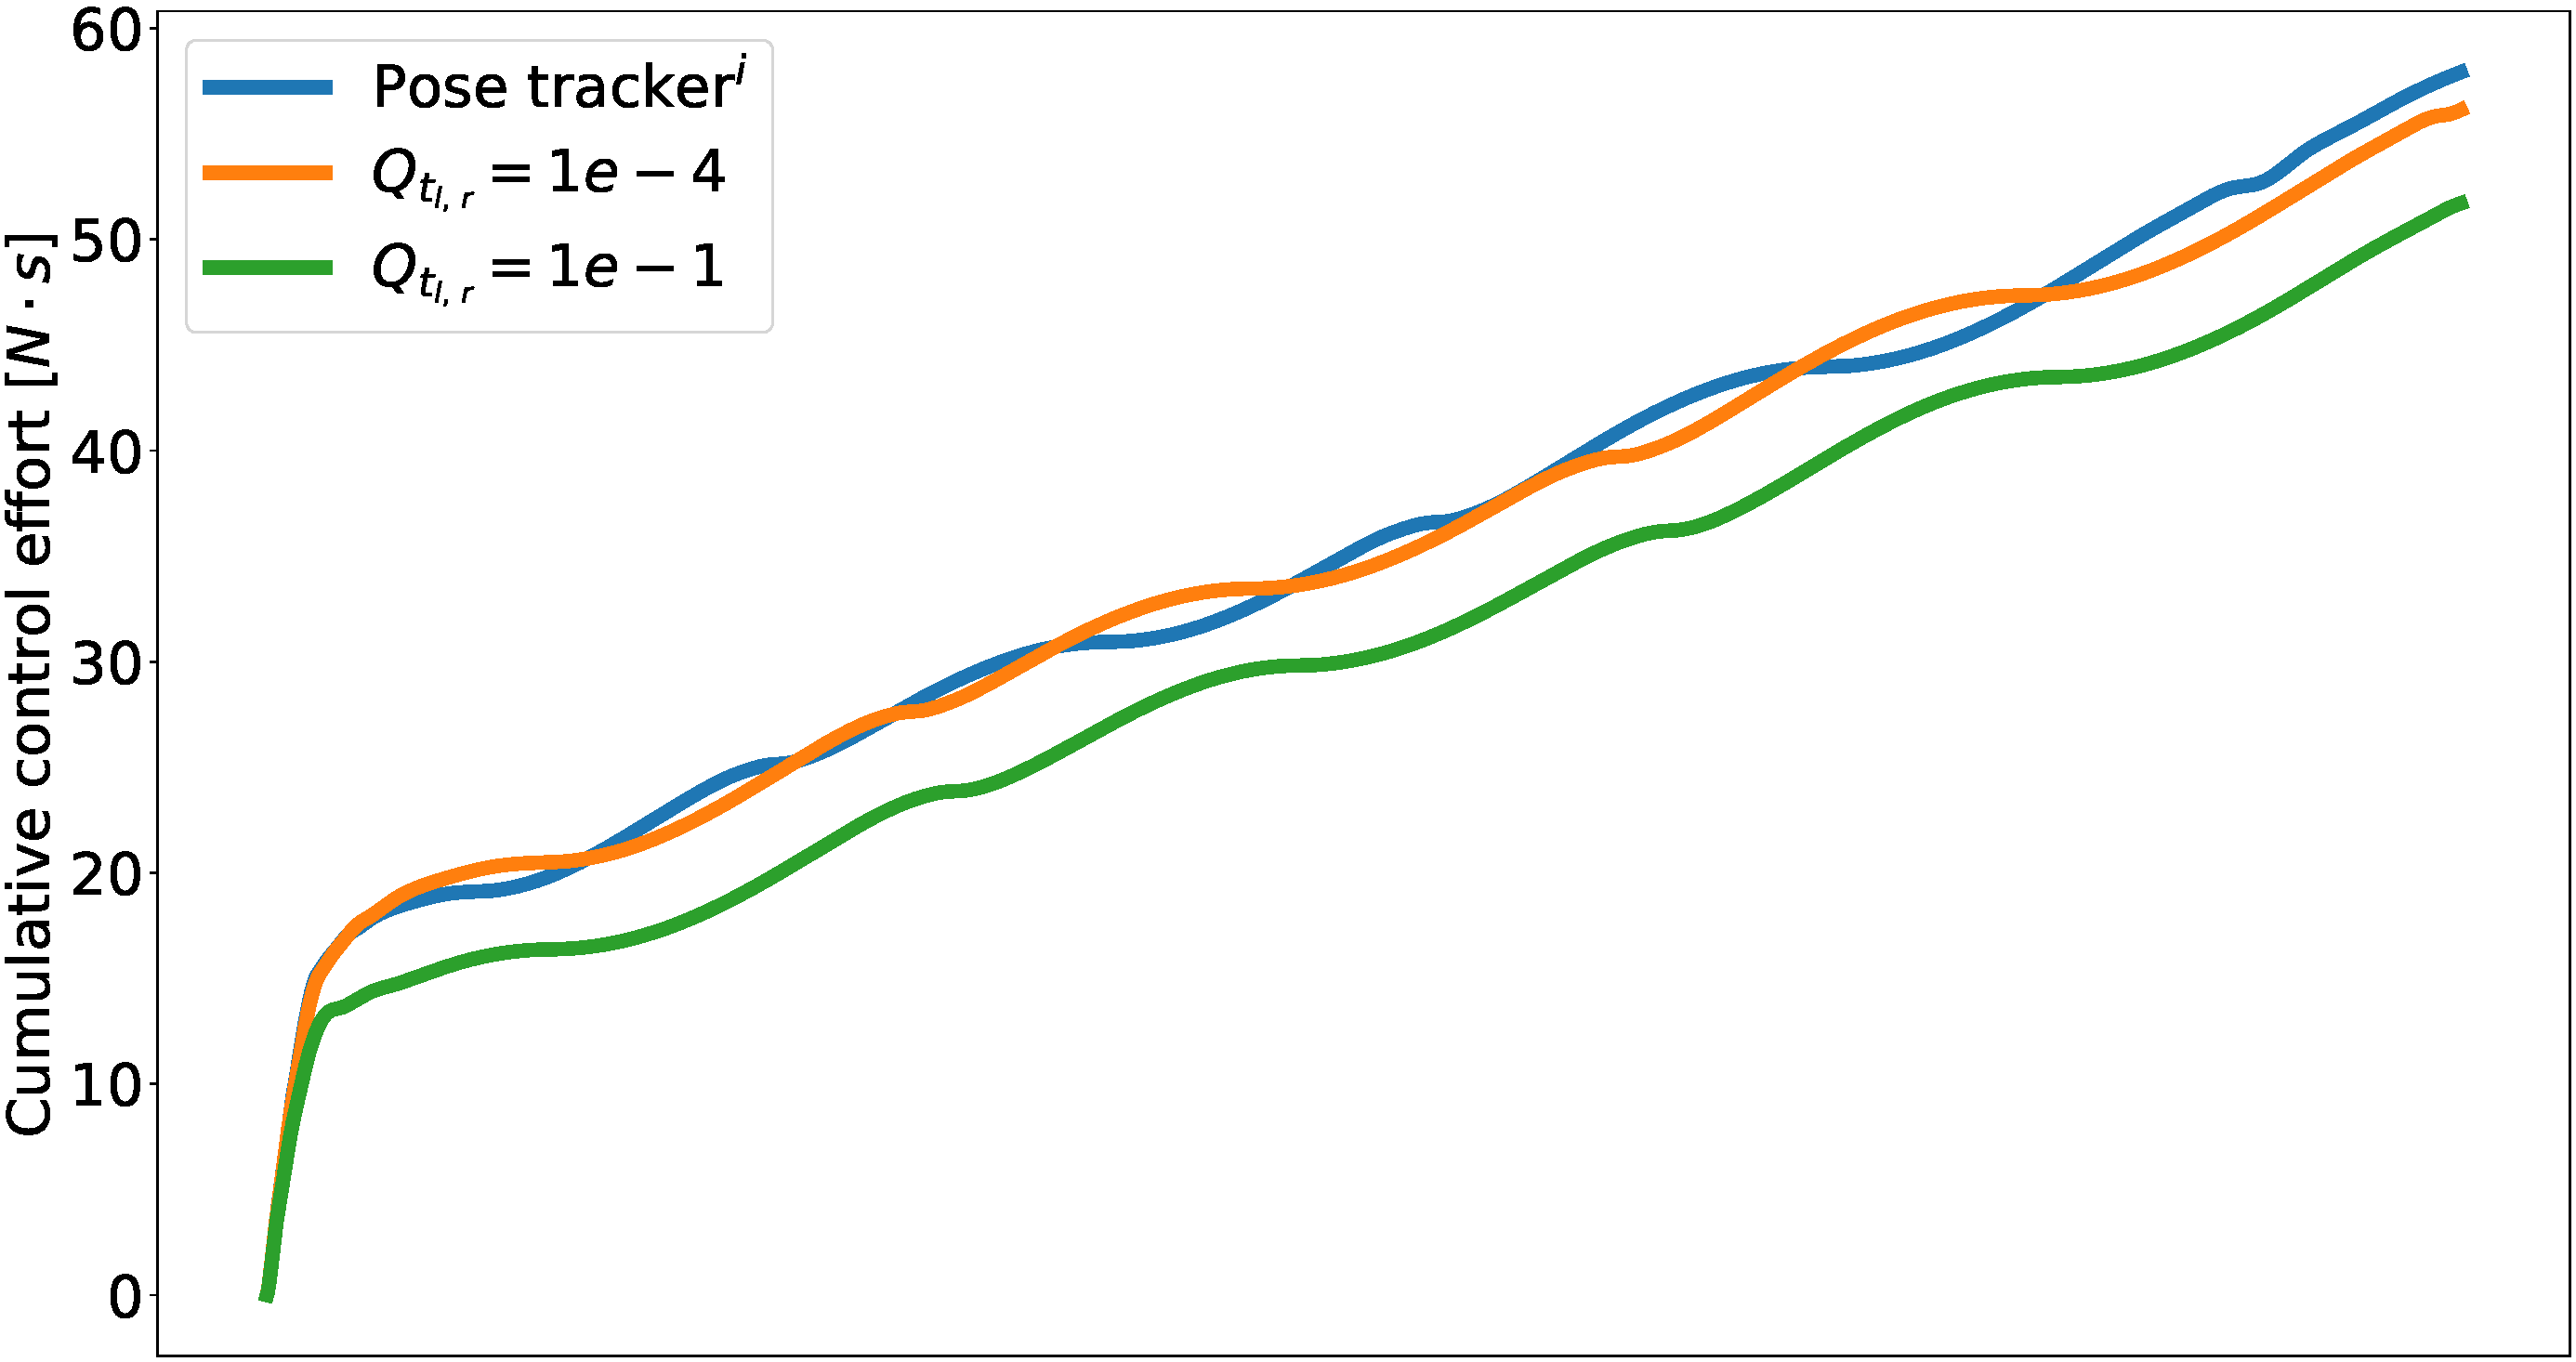
\includegraphics[width=0.49\linewidth]{Figures/Real time one stage planar OCP/Path tracking/forces_cum_sum_comp.pdf}
    \label{subfig:energyrealtimepathtrackingplanarocp}}
  \end{subfigmatrix}
  \caption{Path tracking simulation data.}
  \label{fig:pathtrackingsimdata}
\end{figure}

\subsubsection*{Robustness tests}

Finally, these solvers are subject to robustness tests to evaluate the flexiblity of the proposed solutions to optimally keep tracking the reference, when the mobile robot deviates from it or in case the sensors are affected by noise. Two sets of white gaussian noise are defined and added to the respective states after the vehicle dynamics is forward simulated. As these simulations are affected by white gaussian noise, the control problem becomes stochastic so ten simulations are run for each case.

\begin{figure}[!htb]
  \begin{subfigmatrix}{2}
    \subfigure[$\x,\,\y \sim \mathcal{N}\left(0.0,\,0.01\right),\; \yaw\sim\mathcal{N}\left(0.0,\,0.001\right)$]{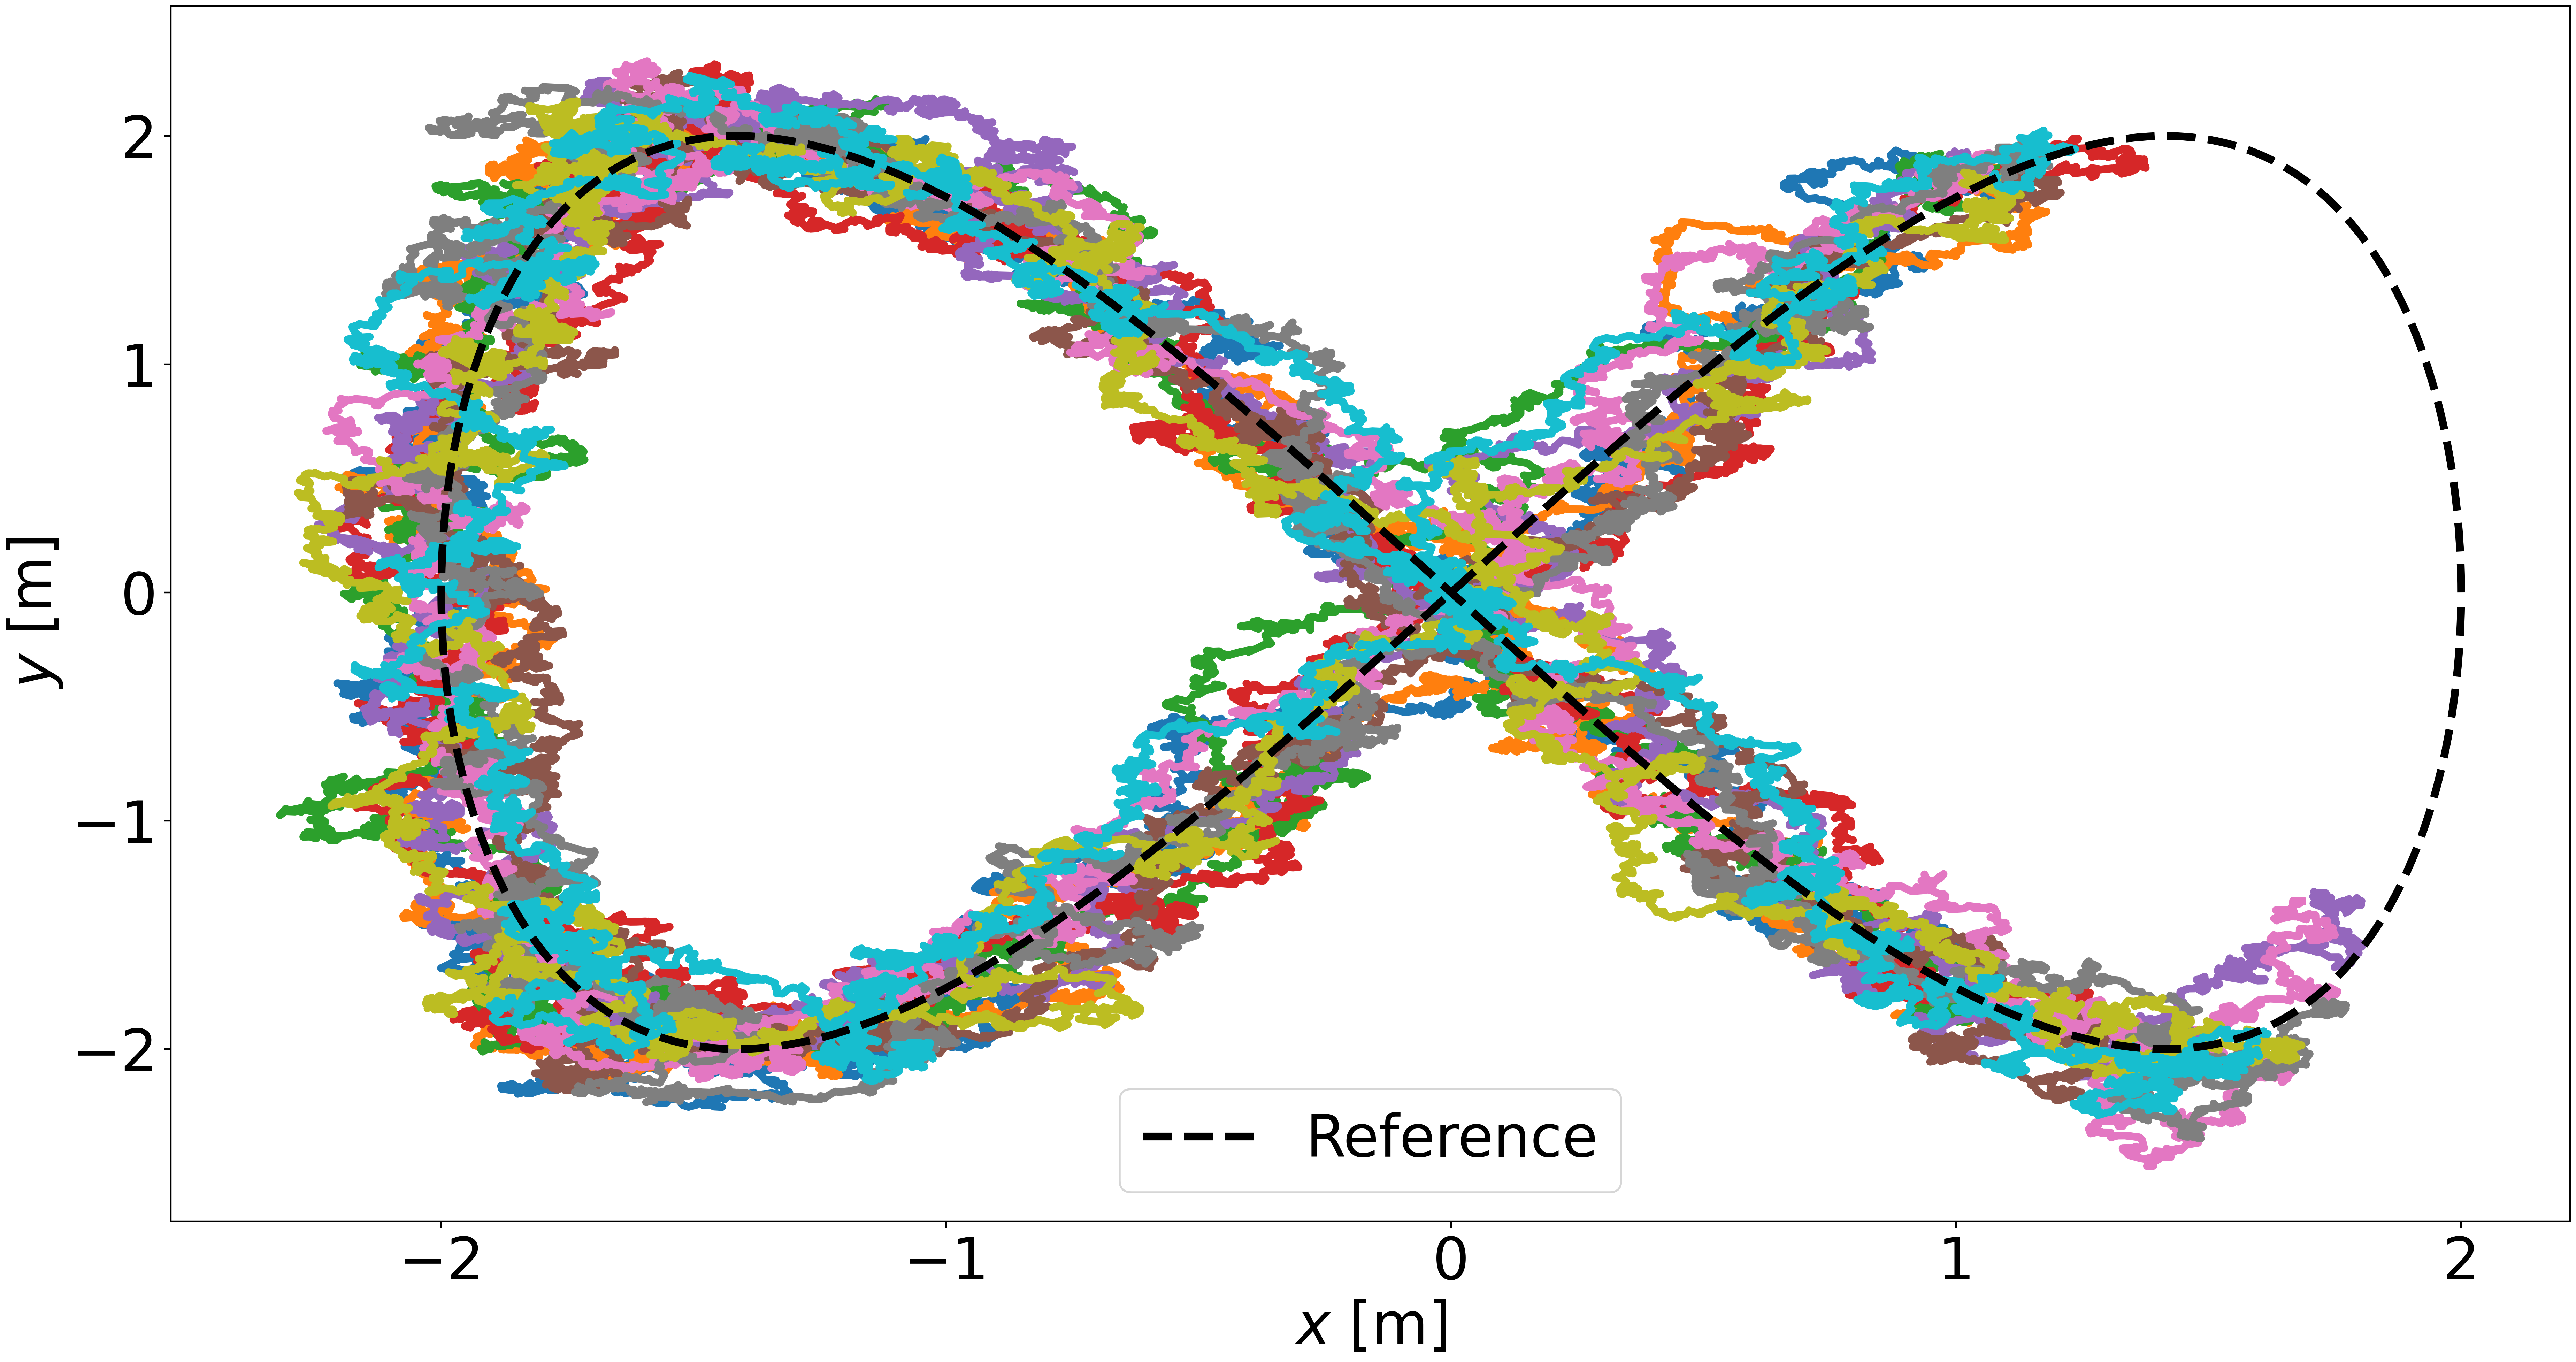
\includegraphics[width=0.49\linewidth]{Figures/Real time one stage planar OCP/Robustness_tests/path_std_noise_position_0.01_std_noise_heading_0.001.png}}
    \subfigure[$\x,\,\y \sim \mathcal{N}\left(0.0,\,0.03\right),\; \yaw\sim\mathcal{N}\left(0.0,\,0.005\right)$]{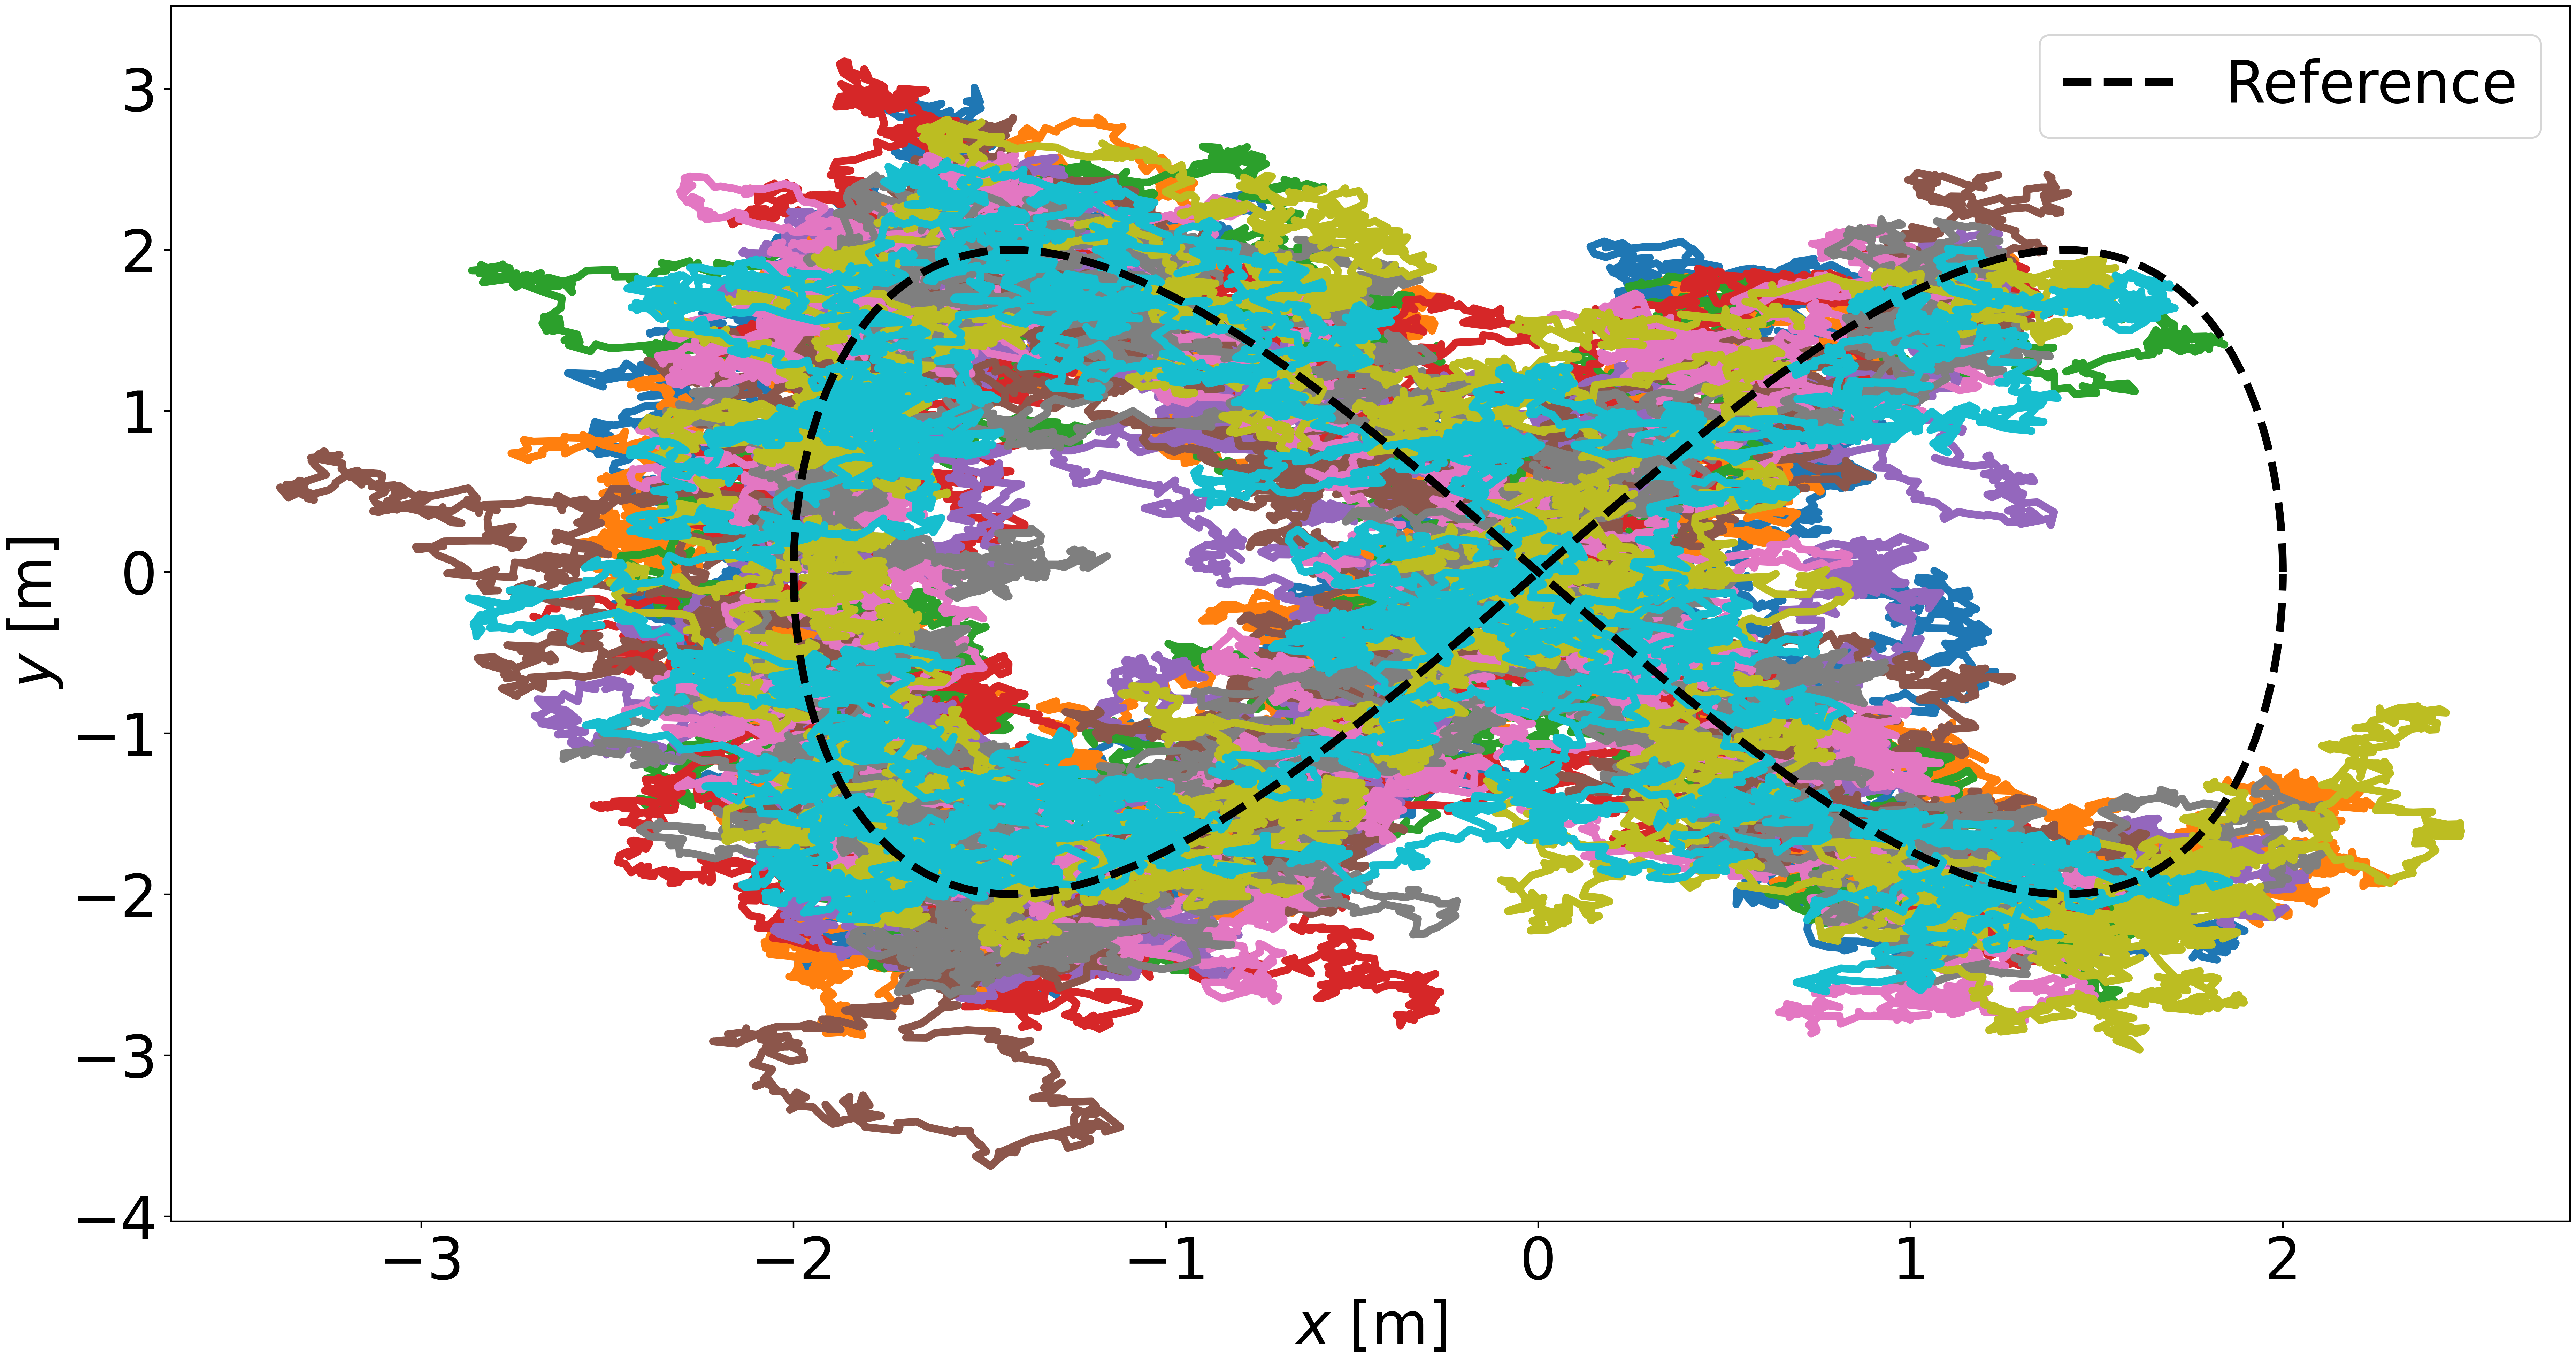
\includegraphics[width=0.49\linewidth]{Figures/Real time one stage planar OCP/Robustness_tests/path_std_noise_position_0.03_std_noise_heading_0.005.png}}
  \end{subfigmatrix}
  \caption{Path tracking simulation subject to noise.}
  \label{fig:pathtrackingsimdatanoise}
\end{figure}

\begin{figure}[!htb]
  \begin{subfigmatrix}{2}
    \subfigure[$\x,\,\y \sim \mathcal{N}\left(0.0,\,0.01\right),\; \yaw\sim\mathcal{N}\left(0.0,\,0.001\right)$]{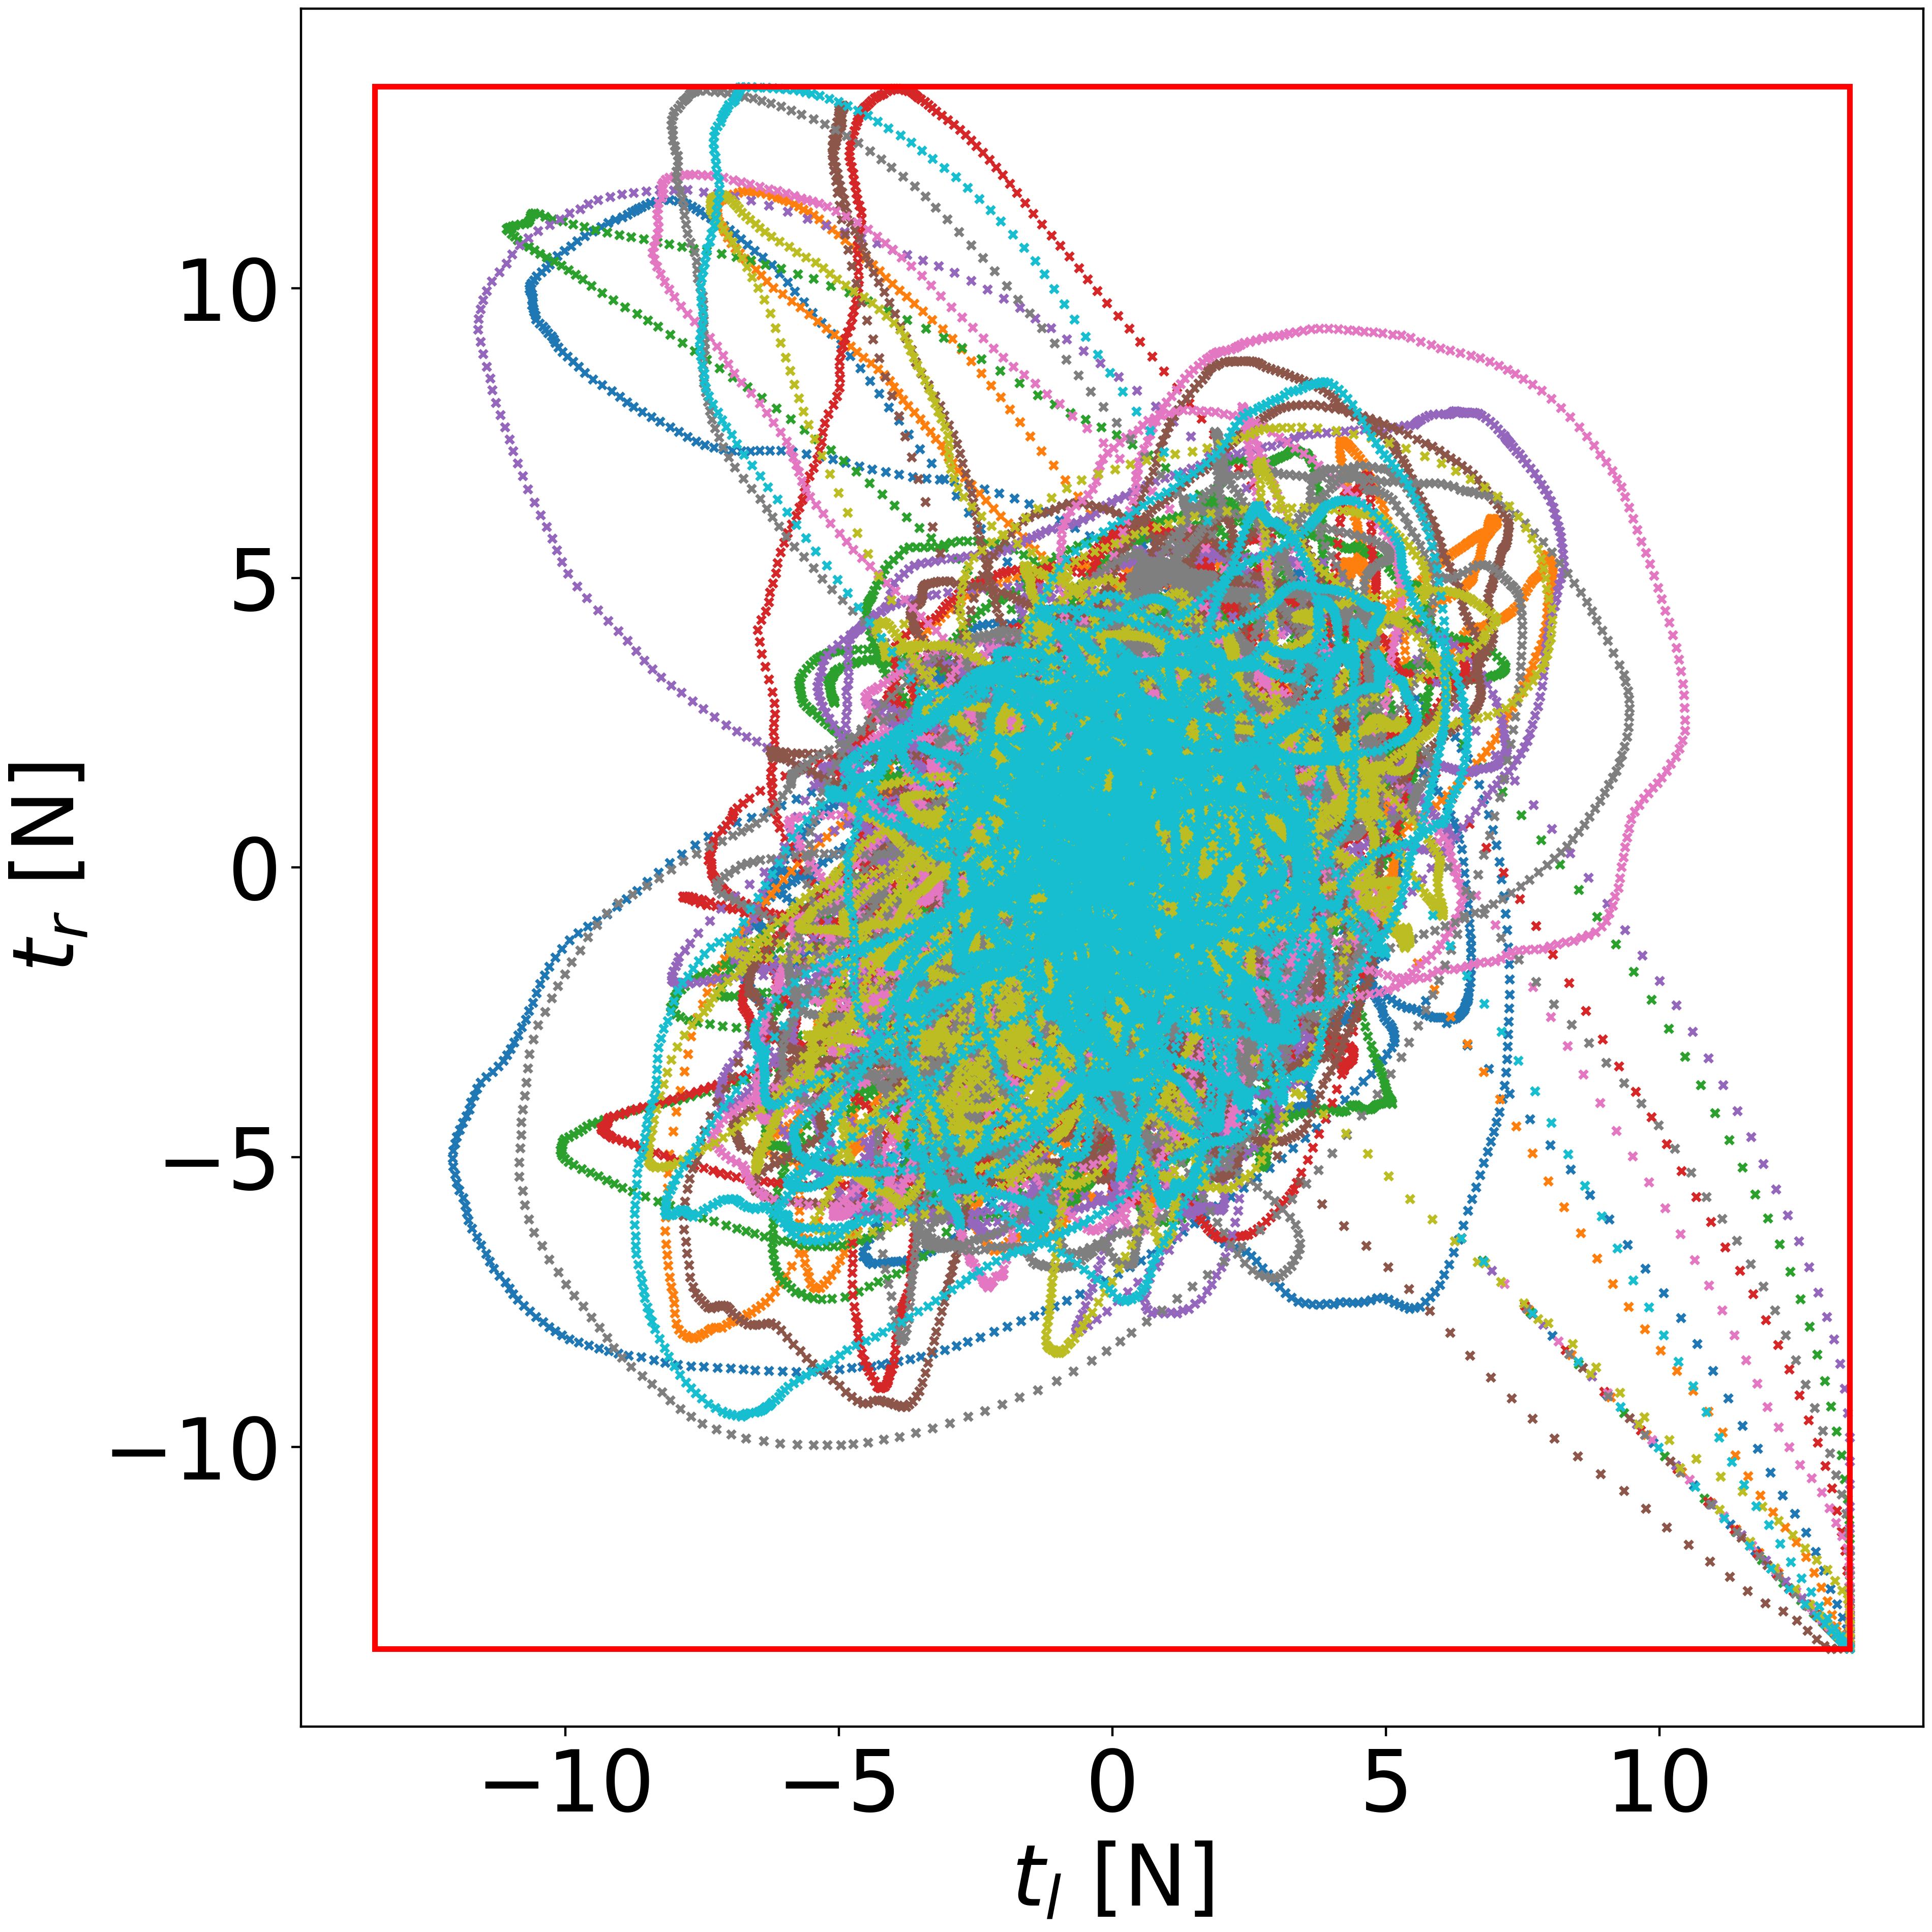
\includegraphics[width=0.49\linewidth]{Figures/Real time one stage planar OCP/Robustness_tests/map_forces_std_noise_position_0.01_std_noise_heading_0.001.png}}
    \subfigure[$\x,\,\y \sim \mathcal{N}\left(0.0,\,0.03\right),\; \yaw\sim\mathcal{N}\left(0.0,\,0.005\right)$]{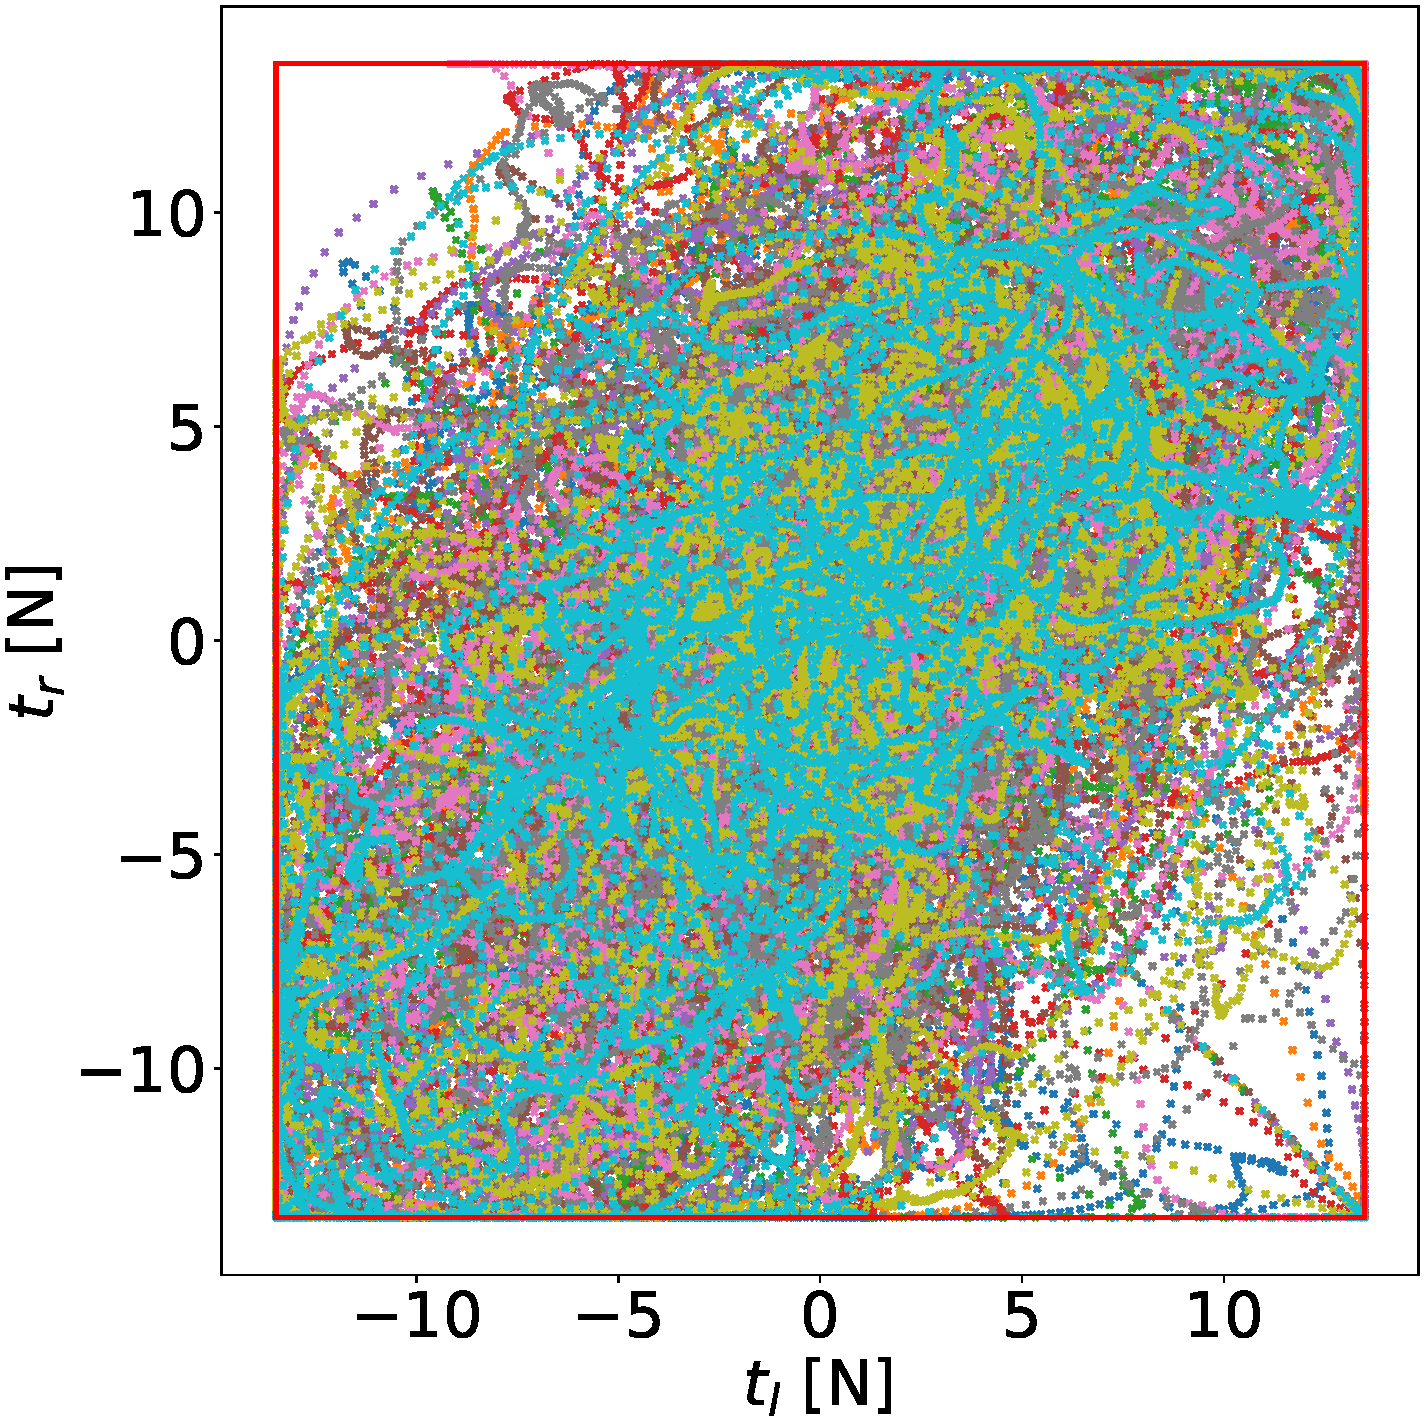
\includegraphics[width=0.49\linewidth]{Figures/Real time one stage planar OCP/Robustness_tests/map_forces_std_noise_position_0.03_std_noise_heading_0.005.png}}
  \end{subfigmatrix}
  \caption{Map of forces.}
  \label{fig:pathtrackingsimdatanoise}
\end{figure}

As expected, when noise amplitude is increased, the tube of positions enlarges and the map of forces shows a more often approximation of forces to its limits, because a greater effort is required from the controller to return the vehicle to the reference.

These simulations aim to take the controller to its limits, so that the \acrshort{nmpc} feasibility is tested under harsh conditions. In every iteration, the solver successfully outputs an optimal solution to the respective \acrshort{nmpc}. However, one shall be careful in case the forces yielded by the controller touch its limits several times, because this may delay the vehicle when it comes to following the reference or introduce wheel slippage in case the vehicle is traversing slopes.

The average loop time among all simulations is always below $5.1$ ms and only a single timeout is recorded (a timeout is considered to happen when the loop time is higher than $T_s$). The computational cost becomes much higher than in the deterministic case, mainly due to significant jumps between consecutive \acrshort{nmpc}s (assumption \ref{assumption:rti3} is not respected).

\begin{remark}
When the mobile robot considerably deviates from the reference, it is advisable to introduce an auxiliary reference to smoothly guide the vehicle back to the main reference. If the vehicle is too far away from the baseline reference, the controller will likely guide the vehicle with high velocities or it may output unstable solutions as the velocities and forces constraints prevent the vehicle from reaching the reference right away. This problem is not directly addressed in this thesis, but it is considered to be solved in case these two references are concatenated into a single continuous reference.
\end{remark}

%%%%%%%%%%%%%%%%%%%%%%%%%%%%%%%%%%%%%%%%%%%%%%%%%%%%%%%%%%%%%%%%%%%%%%%%
\section{Real-time \acrshort{nmpc} over rough terrain}
\label{section:realtimeonestageocproughterrain}

According to the results obtained in the previous section, the \acrshort{nmpc} architecture combined with increasing weight solvers and the virtual speed control module, is tested on a rough terrain scenario, where $\roll \neq 0$ and $\pitch \neq 0$. Firstly, the solvers reaction is tested on a scenario where the mobile robot starts moving on a hill. Secondly, the same solvers are tested against path tracking when $\roll$ and $\pitch$ change abruptly.

This scenario calls for an adaptation of the \acrshort{nmpc} architecture that was used in the planar case. Firstly, the \acrshort{nmpc} must be aware of the vehicle orientation that is imposed by the terrain, namely $\roll$ and $\pitch$. These are continuously measured and provided in advance to the \acrshort{nmpc} (figure \ref{fig:reformarchvspeedoutsideocp}). Moreover, \textbf{one may look to the rough terrain scenario as an extended version of the planar case}. In every situation, the mobile robot needs to take into account the gravity that acts on it. Due to that, the longitudinal wheel force is always equal to the gravity component plus or minus the traction force that is required to follow the respective reference (\refeq{eq:reformSumForces}). Therefore, the solver only needs to find the optimal deviation from the gravity component that enables an optimal reference tracking. Due to that, the state vector becomes $\mathbf{x} = \begin{bmatrix}\x,\,\y,\,\yaw,\,v_x,\,\omega_z,\,\delta\Traction_l,\,\delta\Traction_r\end{bmatrix}^T$. Moreover, $\dot{\delta\Traction}_l = u_l$ and $\dot{\delta\Traction}_r = u_r$. In this section, a Gauss-Newton approximation is used for the hessian. \acrshort{sqprti} is used as solver and partial condensing \texttt{\acrshort{hpipm}} is the \acrshort{qp} solver.

\begin{figure}[!htb]
  \begin{minipage}[c]{0.64\linewidth}
		\tikzstyle{block} = [draw, text centered, minimum height = 2.0em, minimum width = 3.0em, rounded corners, line width = 0.5 mm]
	\begin{tikzpicture}
		\node [block, align= center] at (0.5, 1.3) (1) {\shortstack{Algorithm\\\nameref{alg:determineeulerangles}}};
		\node [block, align= center, draw={rgb,255:red,30;green,145;blue,30}] at (0.7, 0) (2) {\textcolor{rgb,255:red,30;green,145;blue,30}{Virtual speed control}};
		\node [block, align = center] at (4.0, 0) (3) {NMPC\\Dynamics};
		\node [block, align = center] at (7.0, 0) (4) {Plant};
  		\draw [-latex, thick, align = center] (4)
  												 -- ++(1.0, 0.0)
  												 -- ++(0.0, -1.1)
  												 -- coordinate (bottomSeg) node [above, xshift=-2em] {$\mathbf{\hat{x}}_0$} ++(-9.4, 0.0)
  												 -- ++(0.0, 1.1) coordinate (point2)
  												 -- (2);
    	\coordinate (pointBelow3) at ($(3 |- bottomSeg)$);
    	\filldraw[black] (pointBelow3) circle (1pt);
    	\filldraw[black] (point2) circle (1pt);
  		\draw [-latex, thick, align=center] ([yshift=4.0]3.east)
		-- ++(0.15, 0.0)
		-- ++(0.0, 0.7)
		-- node[above] {$\mathbf{x}^*,\,\mathbf{u}^*$} ++(-0.8, 0.0)
		-- (3);
		
		\draw [-latex, thick, align=center] (1)
		-- node [above] {$\hat{\roll}_0,\,\hat{\pitch}_0$} ++(3.0, 0.0)
		-- (3);
		
  		\draw [-latex,thick] (2) -- node [above] {$\mathbf{r}$} (3);
  		\draw [-latex,thick] (3) -- node [above] {$\mathbf{u}_0^*$} (4);
  		\draw [-latex, thick] (pointBelow3) -- (3);
  		\draw [-latex, thick] (point2)
  			-- ++(0.0, 1.3)
  			-- (1);
  		
  		
	\end{tikzpicture}
  \end{minipage}
  \begin{minipage}[c]{0.34\linewidth}
  	\begin{equation}
		\begin{cases}
			\Traction_l &= \frac{mg\sin(\theta)}{4} + \delta\,\Traction_l\\
			\Traction_r &= \frac{mg\sin(\theta)}{4} + \delta\,\Traction_r 
		\end{cases}
		\label{eq:reformSumForces}
	\end{equation}
  \end{minipage}
\caption{\acrshort{nmpc} adapted to a rough terrain environment. The \textcolor{tabvs}{virtual speed control module} is detailed in figure \ref{fig:virtual_speed_module_qp}.}
\label{fig:reformarchvspeedoutsideocp}
\end{figure}

The determination of the roll and pitch angles is outlined in section \ref{section:eulerAnglesDetermination}. In this case it is done analytically, but may be replaced by data from sensors. Then, some white gaussian noise is added to the determined values in order to simulate rough, uneven terrain.
\begin{subequations}
	\begin{align}
		\hat{\roll}_0 &= \roll_0 + \epsilon_{\roll}, \; \epsilon_{\roll} \sim \mathcal{N}\left(0.0,\,\sigma_{\roll}^2\right)\\
		\hat{\pitch}_0 &= \pitch_0 + \epsilon_{\pitch}, \; \epsilon_{\pitch} \sim \mathcal{N}\left(0.0,\,\sigma_{\pitch}^2\right)
	\end{align}
\end{subequations}
\subsection{Moving on hill}
\label{subsection:hill}

The mobile robot is placed on a hill of type $h\left(\x,\,\y\right) = a\,x$, where $a$ sets the hill steepness. The virtual speed control module is made of equations \eqref{eq:vspeed_computation_architecture_b} and \eqref{eq:virtualspeedqp}. Table \ref{tab:hillPathTrackingSpecs} presents the parameters of the solvers that are used in this subsection. Figure \ref{fig:pathCompHills} presents the path tracking results to a straight line while traversing the hill, whereas the right side of it presents the roll and pitch angles the mobile robot was subject to during this traversal.

\begin{table}[!htb]
  \caption[Solver parameters on hill.]{Path tracking solver parameters ($N = 50,\; T_s = 10\,ms$).}
  \label{tab:hillPathTrackingSpecs}
  \renewcommand{\arraystretch}{1.1}
  \centering
  \begin{tabular}[]{lcc}
	\toprule
		& $Q_i$ & $R$\\
	\midrule
	(1) Pose tracker & $diag\left(3.0 \cdot \mathbf{1}_3,\,1\mathrm{e}{-9} \cdot \mathbf{1}_4\right)$ & $1\mathrm{e}{-3}\cdot \mathbf{1}_2$\\
	(2) Energy saver & $diag\left(3.0\times 1.1^i \cdot \mathbf{1}_3,\,1\mathrm{e}{-9} \cdot \mathbf{1}_2,\,1\mathrm{e}{-4}\cdot\mathbf{1}_2\right)$ & $1\mathrm{e}{-3}\cdot \mathbf{1}_2$\\
	\end{tabular}
	\begin{tabular}[]{cccccc}
  	\toprule
  	$\left[(v_x)_{min},\; (v_x)_{max}\right]\,[m/s]$ & $\left[(\omega_z)_{min},\; (\omega_z)_{max}\right]\,[rad/s]$ & $\left[(u_i)_{min},\,(u_i)_{max}\right]\,[N \cdot s]$ & $\FrictionCoefficient$ & $\sigma_{\roll}$ & $\sigma_{\pitch}$\\
  	\midrule
  	$\left[-5.0,\,5.0\right]$ & $\left[-5.0,\,5.0\right]$ & $\left[-100,\,100\right]$ & $0.7$ & $7\mathrm{e}{-2}$ & $7\mathrm{e}{-2}$\\
  	\bottomrule
  \end{tabular}
\end{table}

\begin{figure}[!htb]
  \begin{subfigmatrix}{2}
    \subfigure[Path tracking over hill with different conditions.]{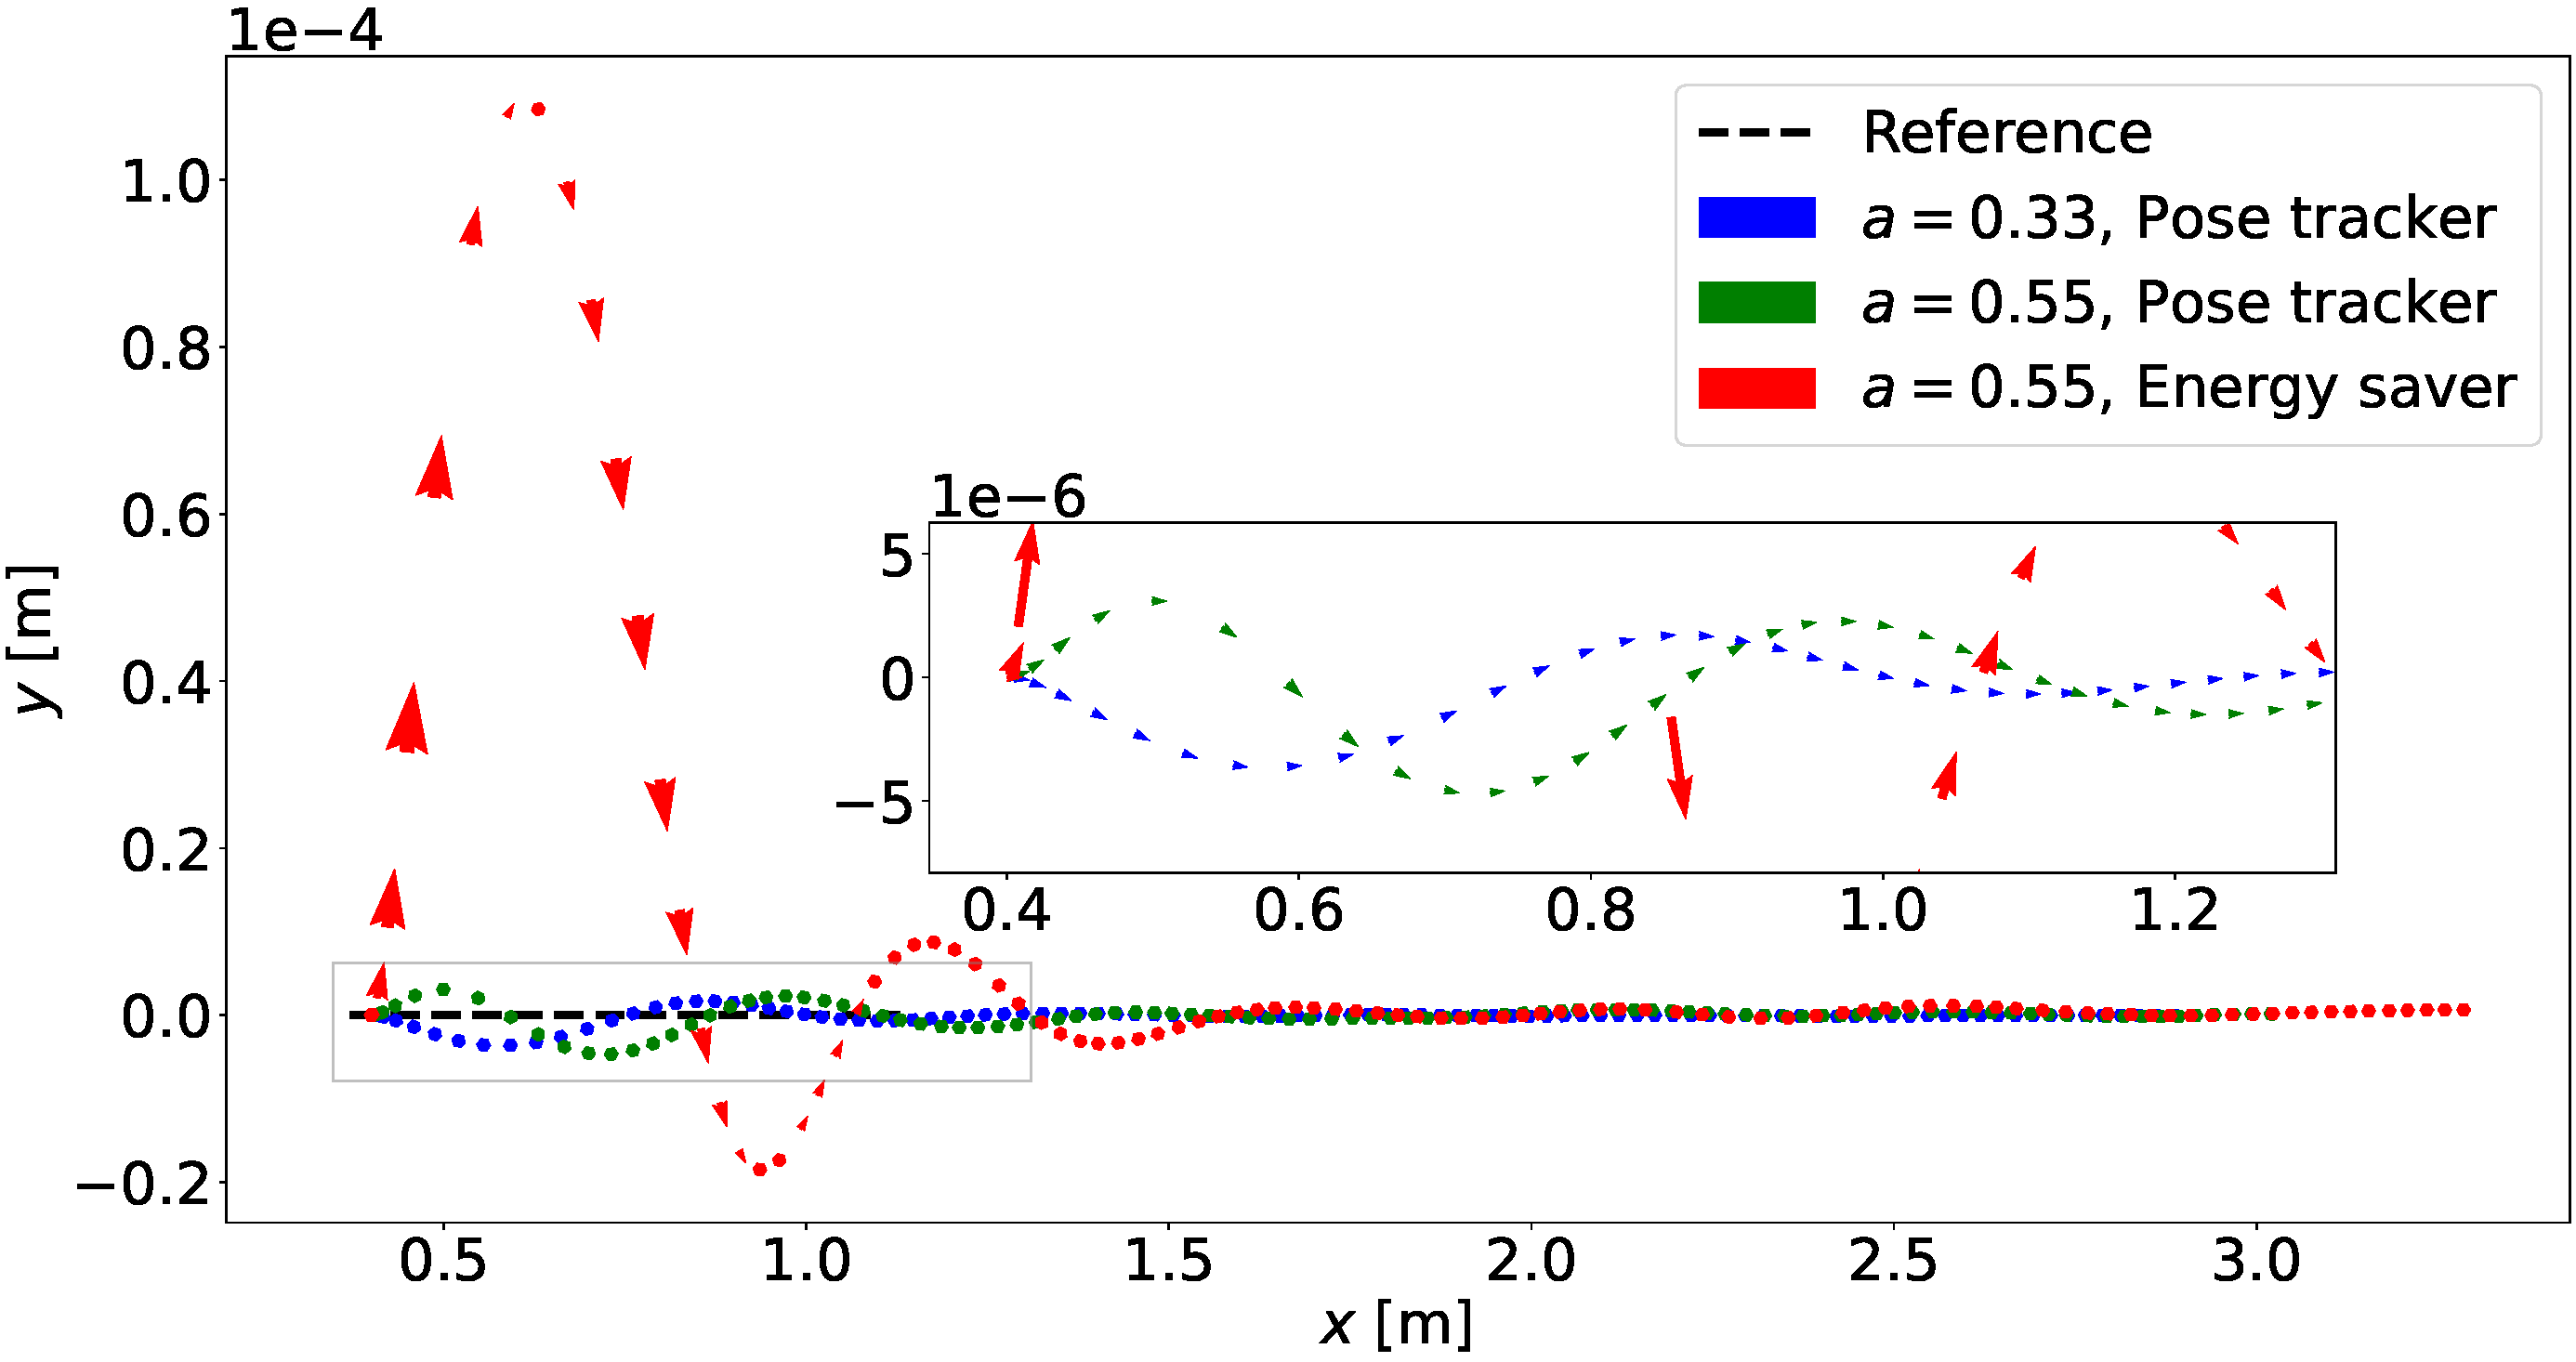
\includegraphics[width=0.49\linewidth]{Figures/Real time one stage OCP on rough terrain/Hill/Path tracking comparison among hills.pdf}}
    \subfigure[Pitch \textcolor{orange}{(orange)} and roll \textcolor{blue}{(blue)}. $a=0.3$ (top) and $a=0.55$ (bottom).]{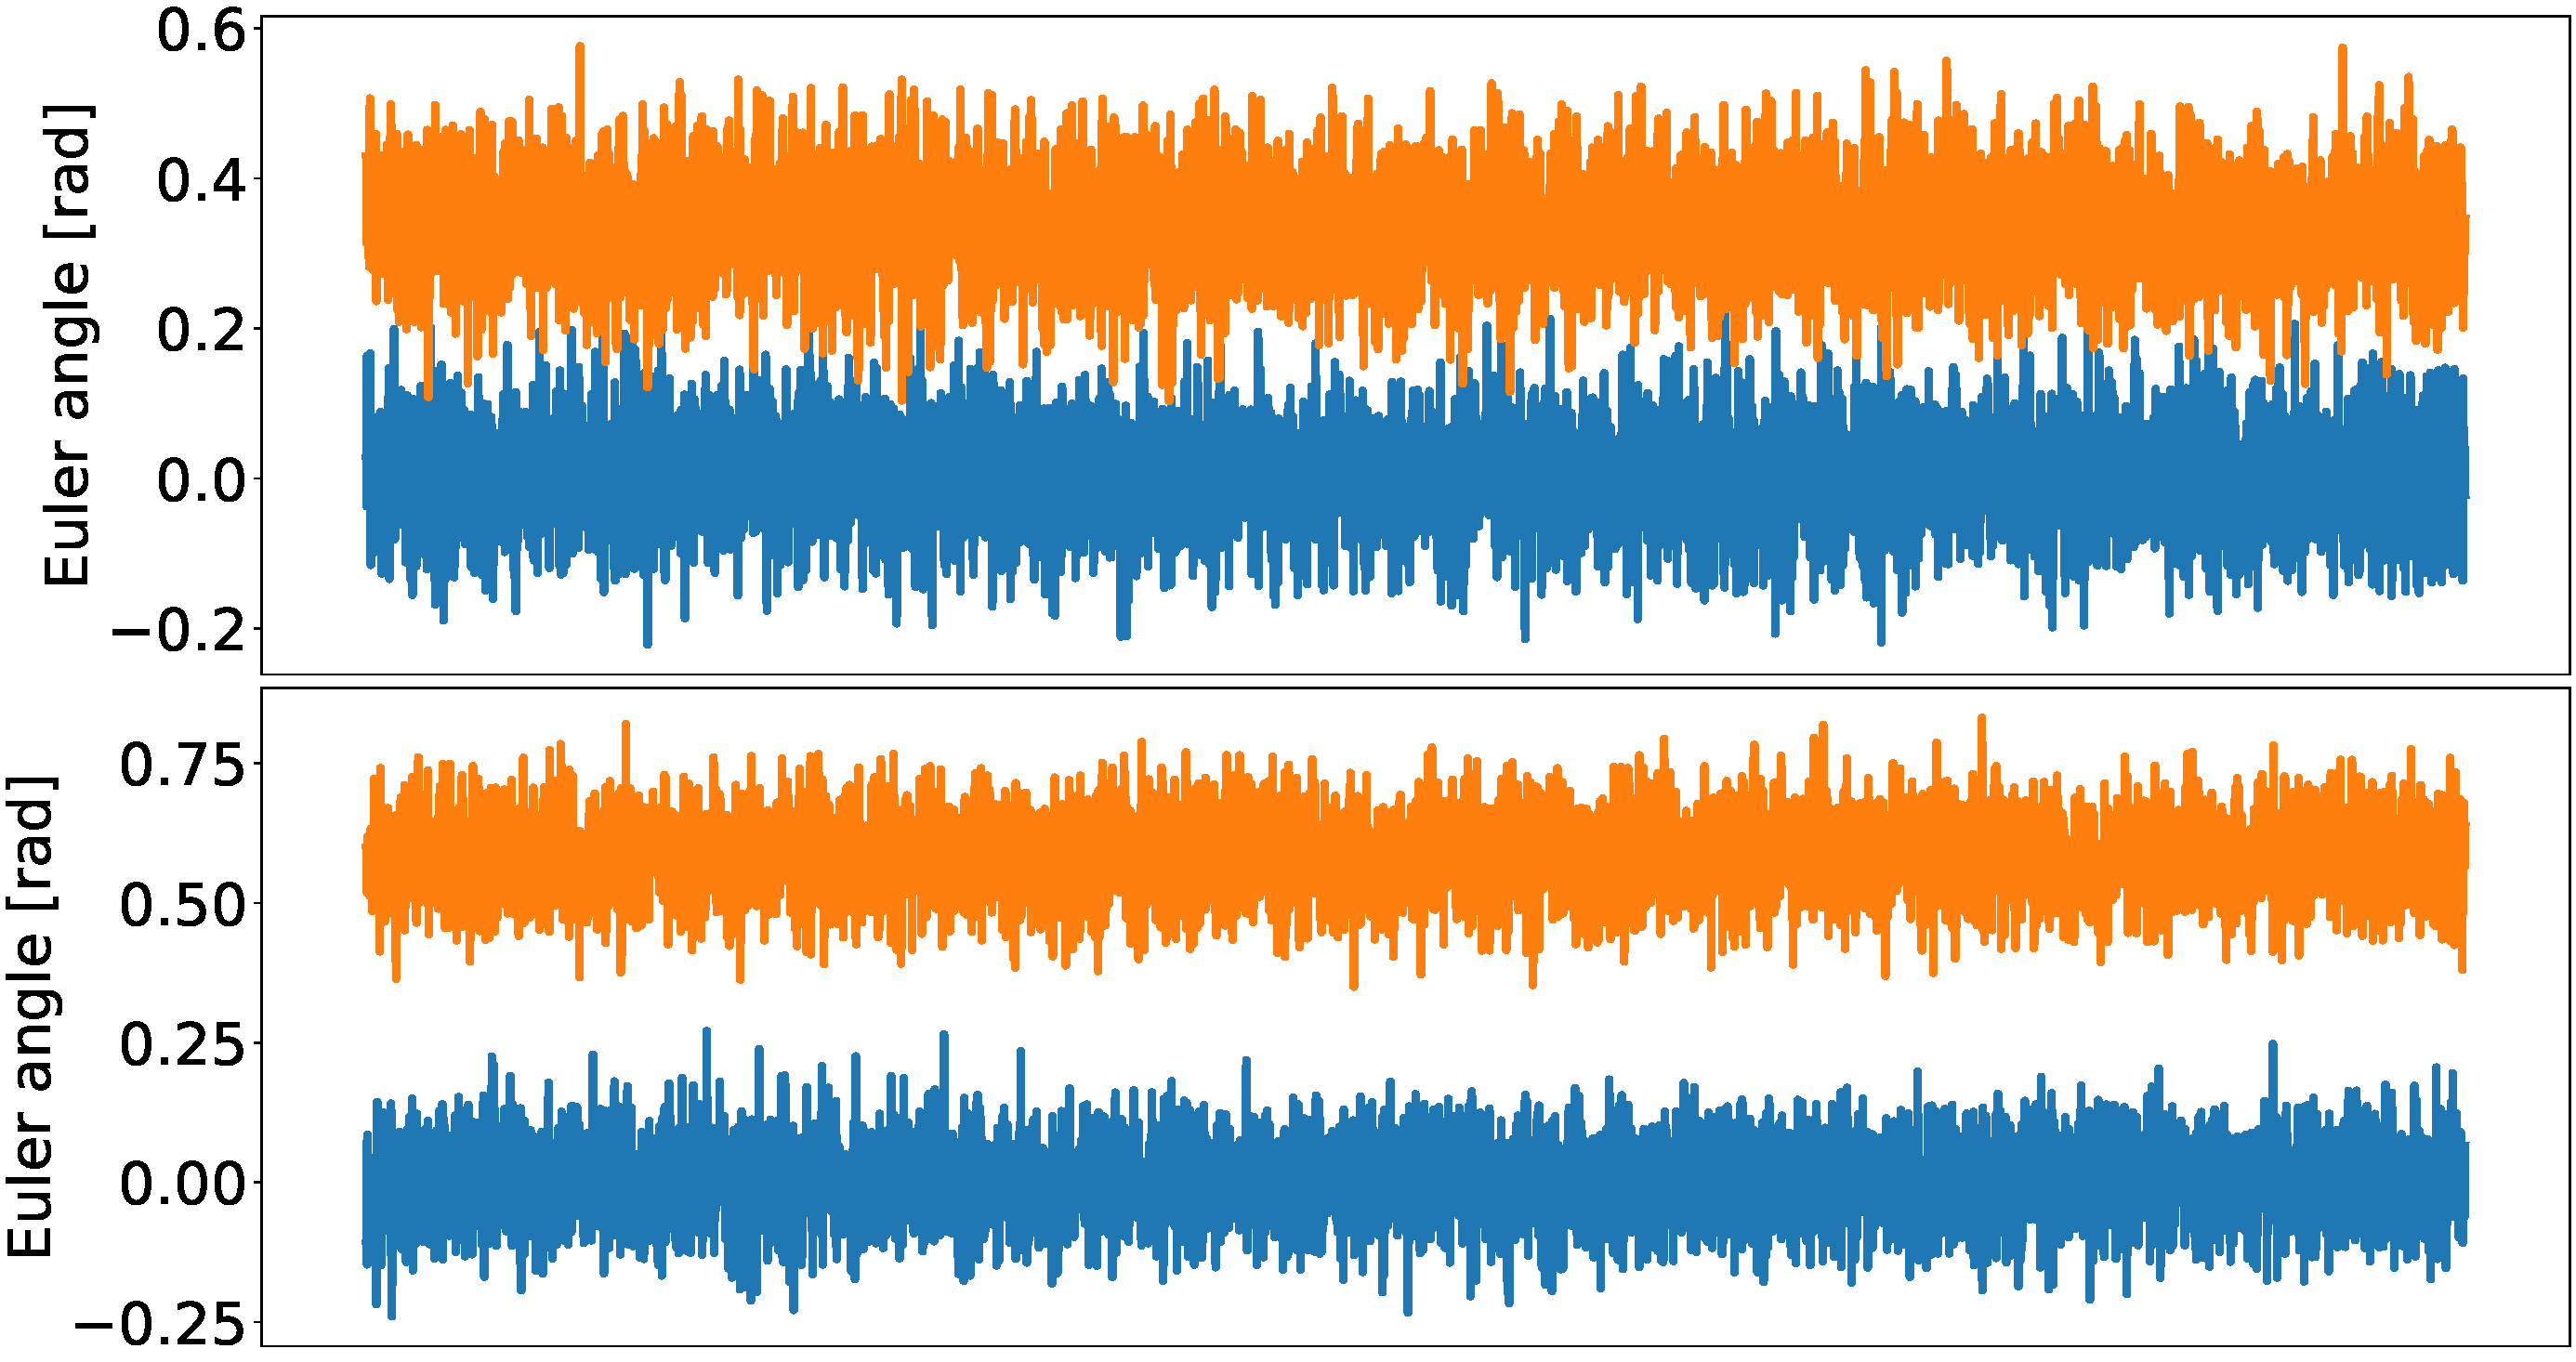
\includegraphics[width=0.49\linewidth]{Figures/Real time one stage OCP on rough terrain/Hill/roll_pitch_hill.pdf}}
  \end{subfigmatrix}
  \caption{Path tracking over hill with rough, uneven terrain.}
  \label{fig:pathCompHills}
\end{figure}

The adapted \acrshort{nmpc} architecture has proven to work well under the new scenario. As expected, the controller tracks the reference pose. However, the controller outputs different optimal controls according to the terrain steepness. Figure \ref{fig:ForcesConeHill} presents the position of the wheel traction forces in the Coulomb friction cone. If the norm of the wheel traction force vector is in the light green area, there is no wheel slippage. On the other hand, in case the traction force norm is in the light red area, wheel slippage arises.

\begin{figure}[!htb]
  \begin{subfigmatrix}{3}
    \subfigure[$a=0.33$, Pose tracker.]{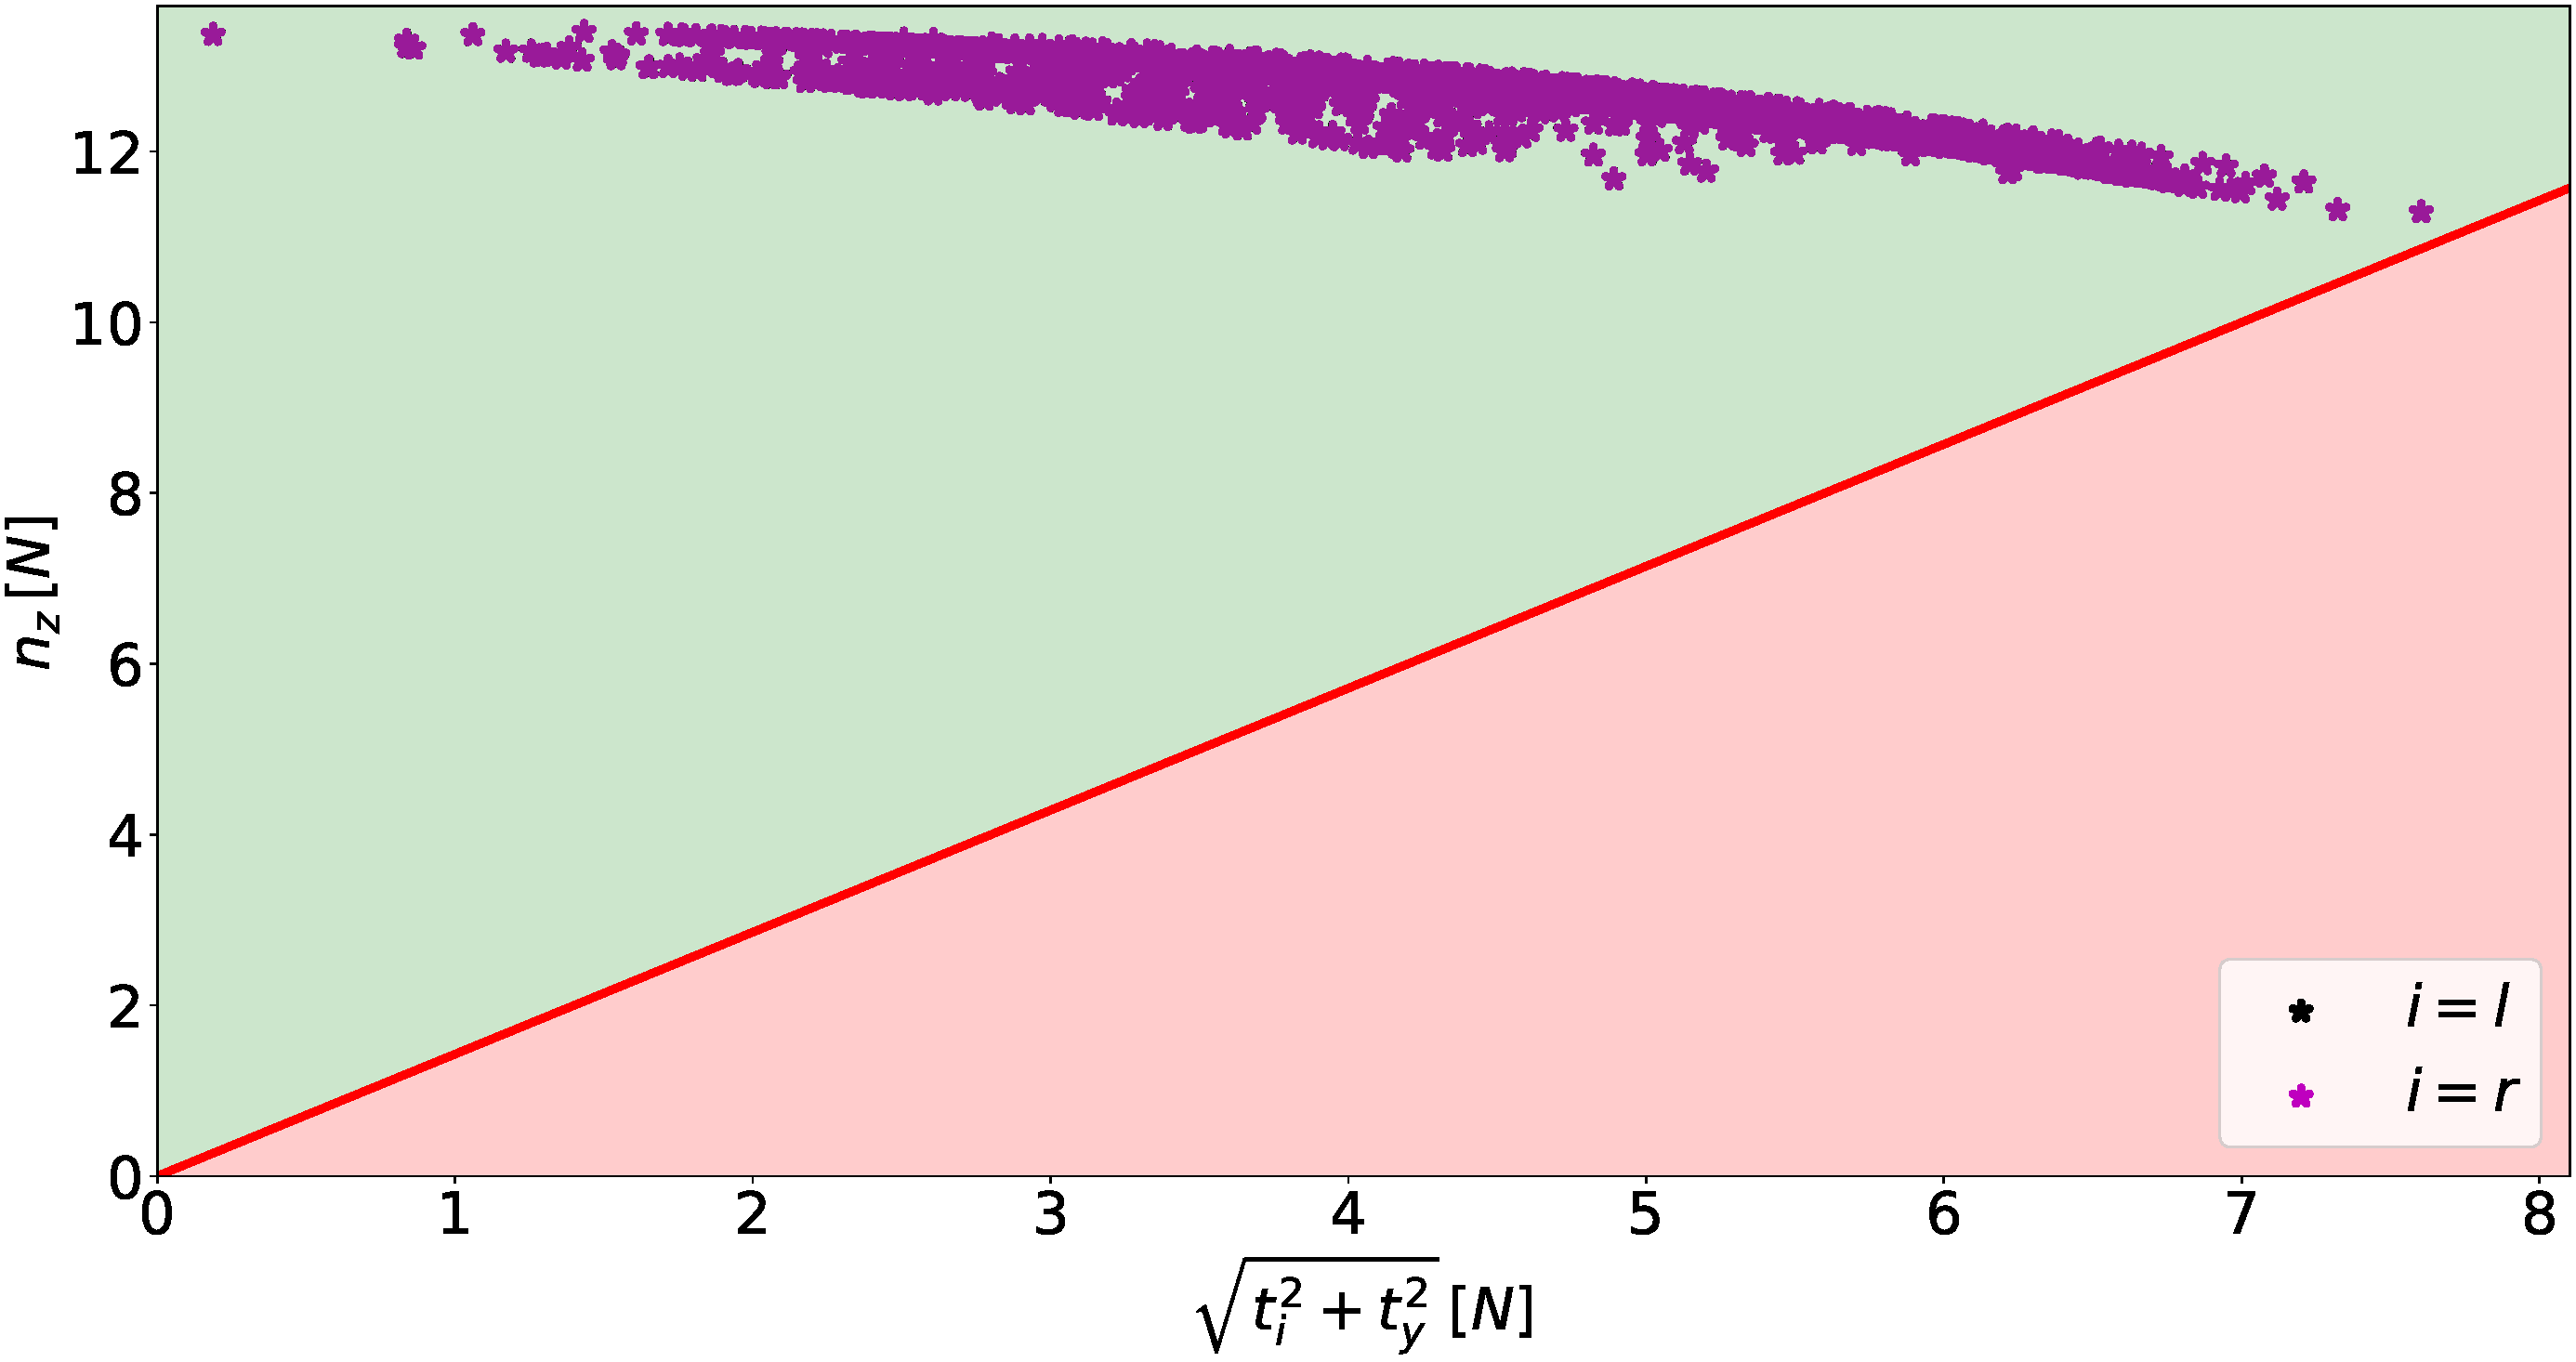
\includegraphics[width=0.31\linewidth]{Figures/Real time one stage OCP on rough terrain/Hill/forces_cone_a_33_1.pdf}}
    \subfigure[$a=0.55$, Pose tracker.]{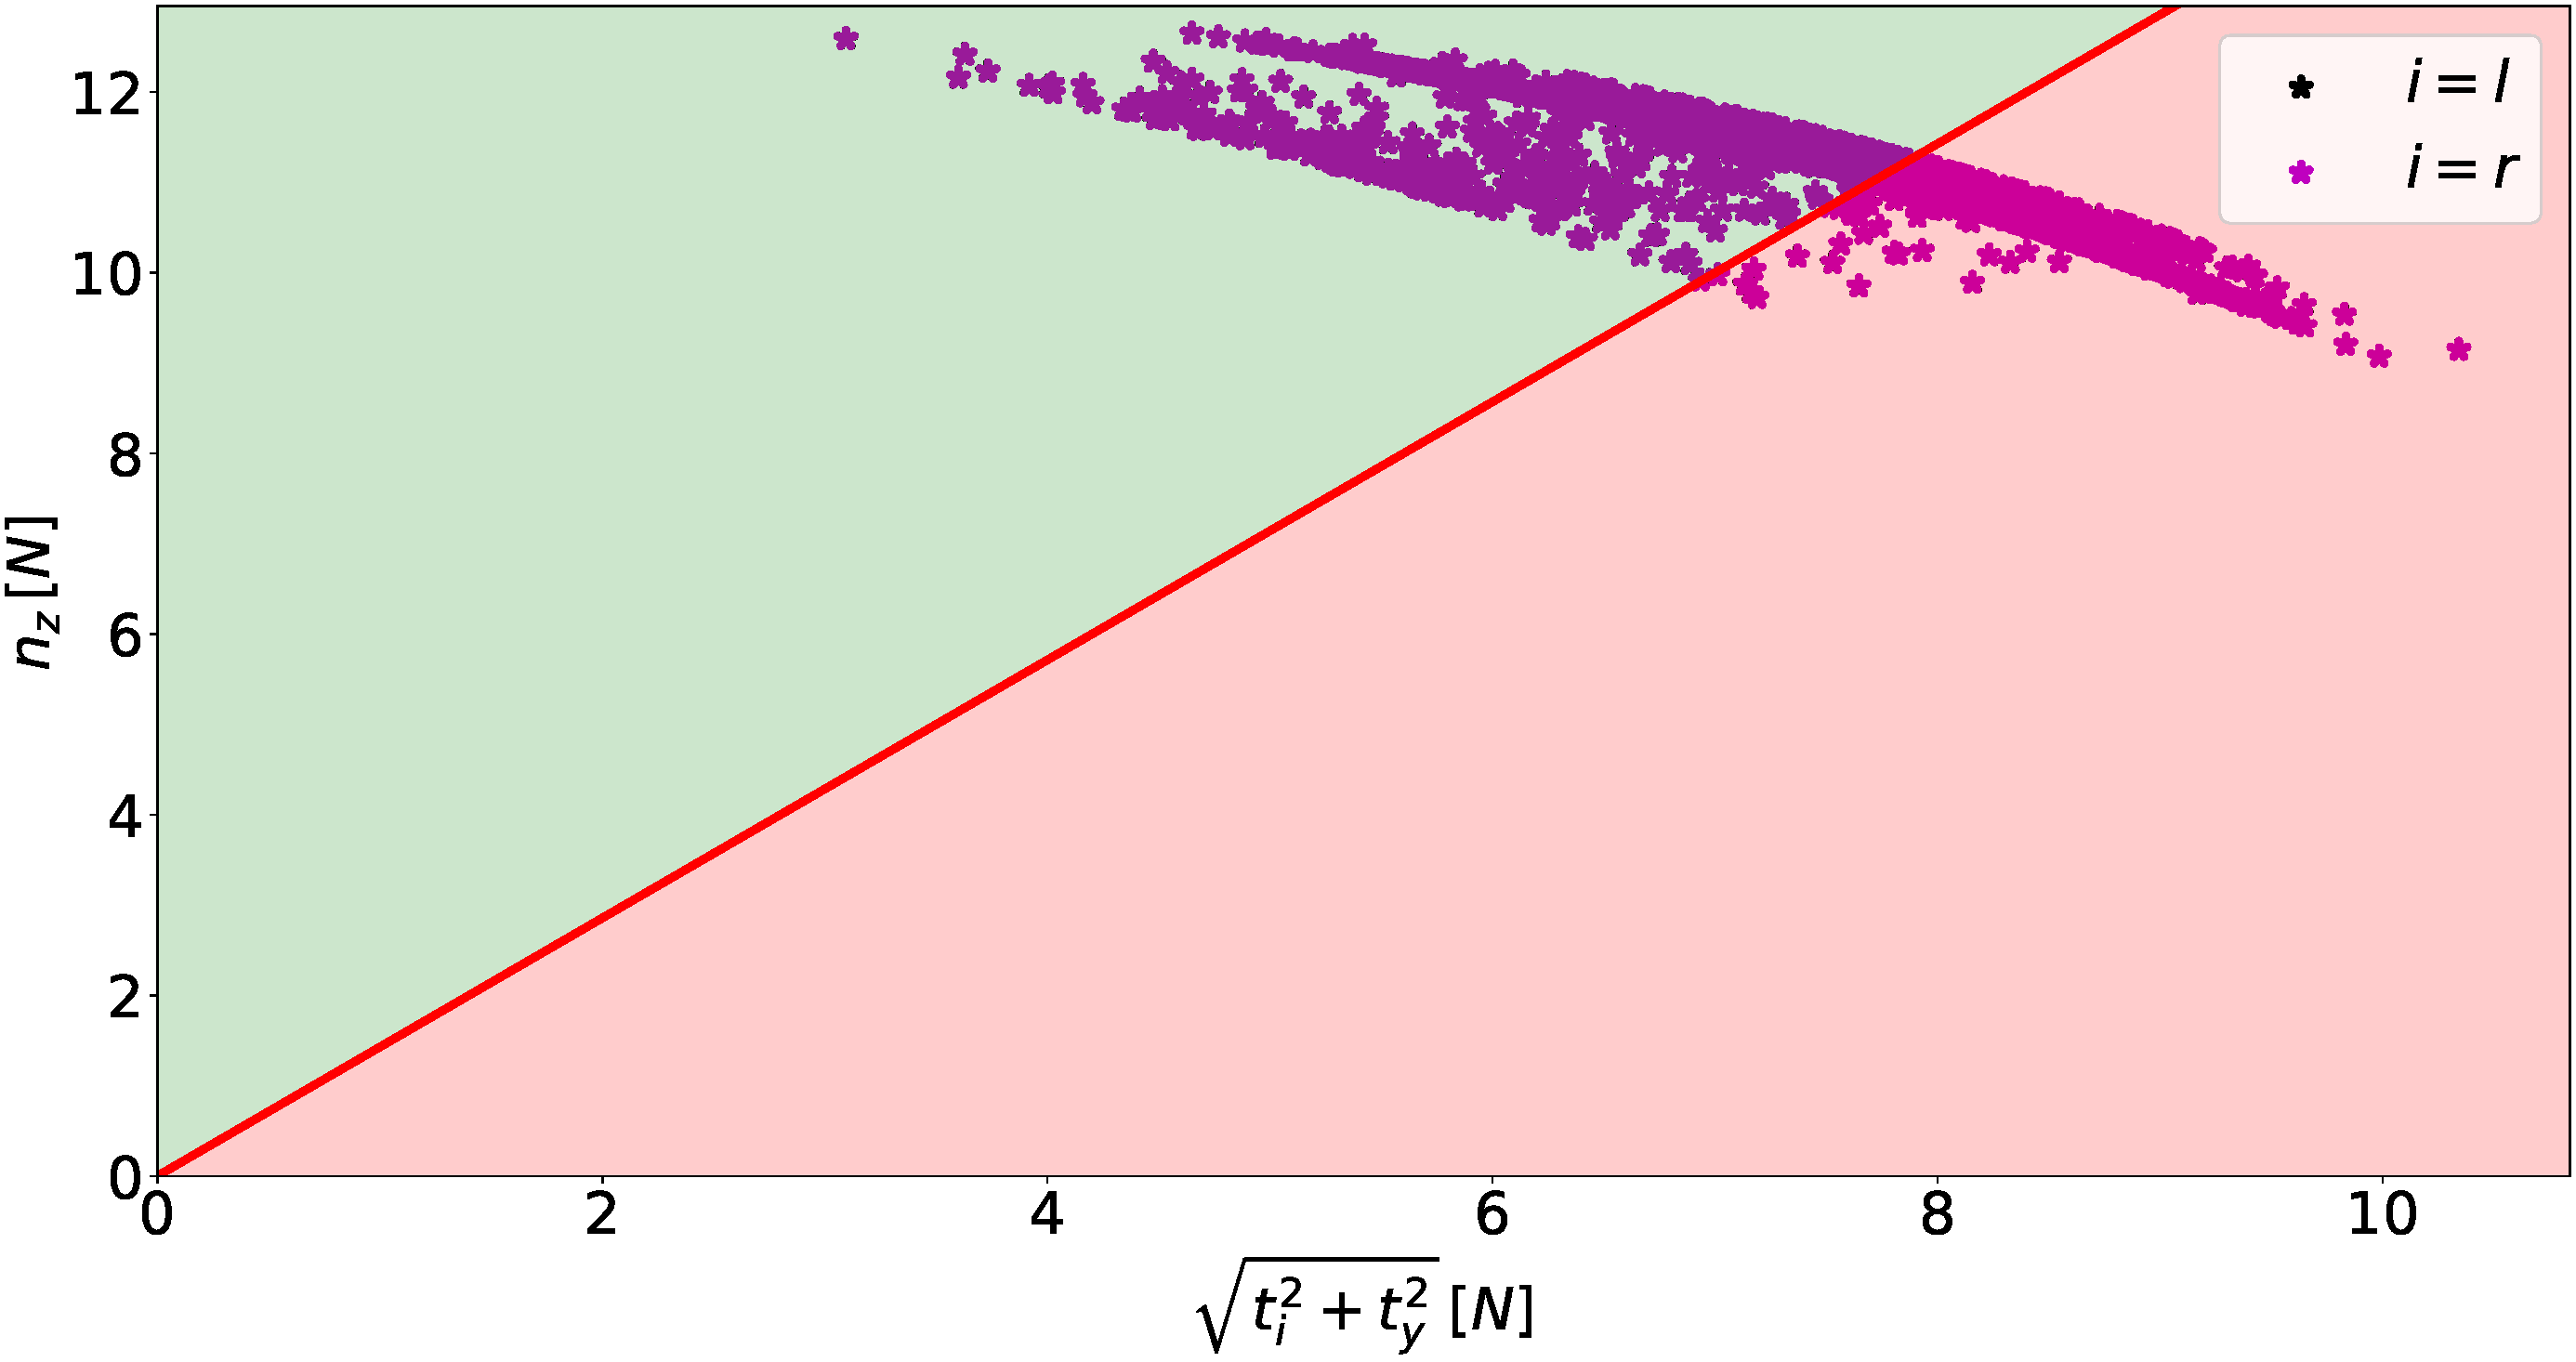
\includegraphics[width=0.31\linewidth]{Figures/Real time one stage OCP on rough terrain/Hill/forces_cone_a_55_1.pdf}}
    \subfigure[$a=0.55$, Energy saver.]{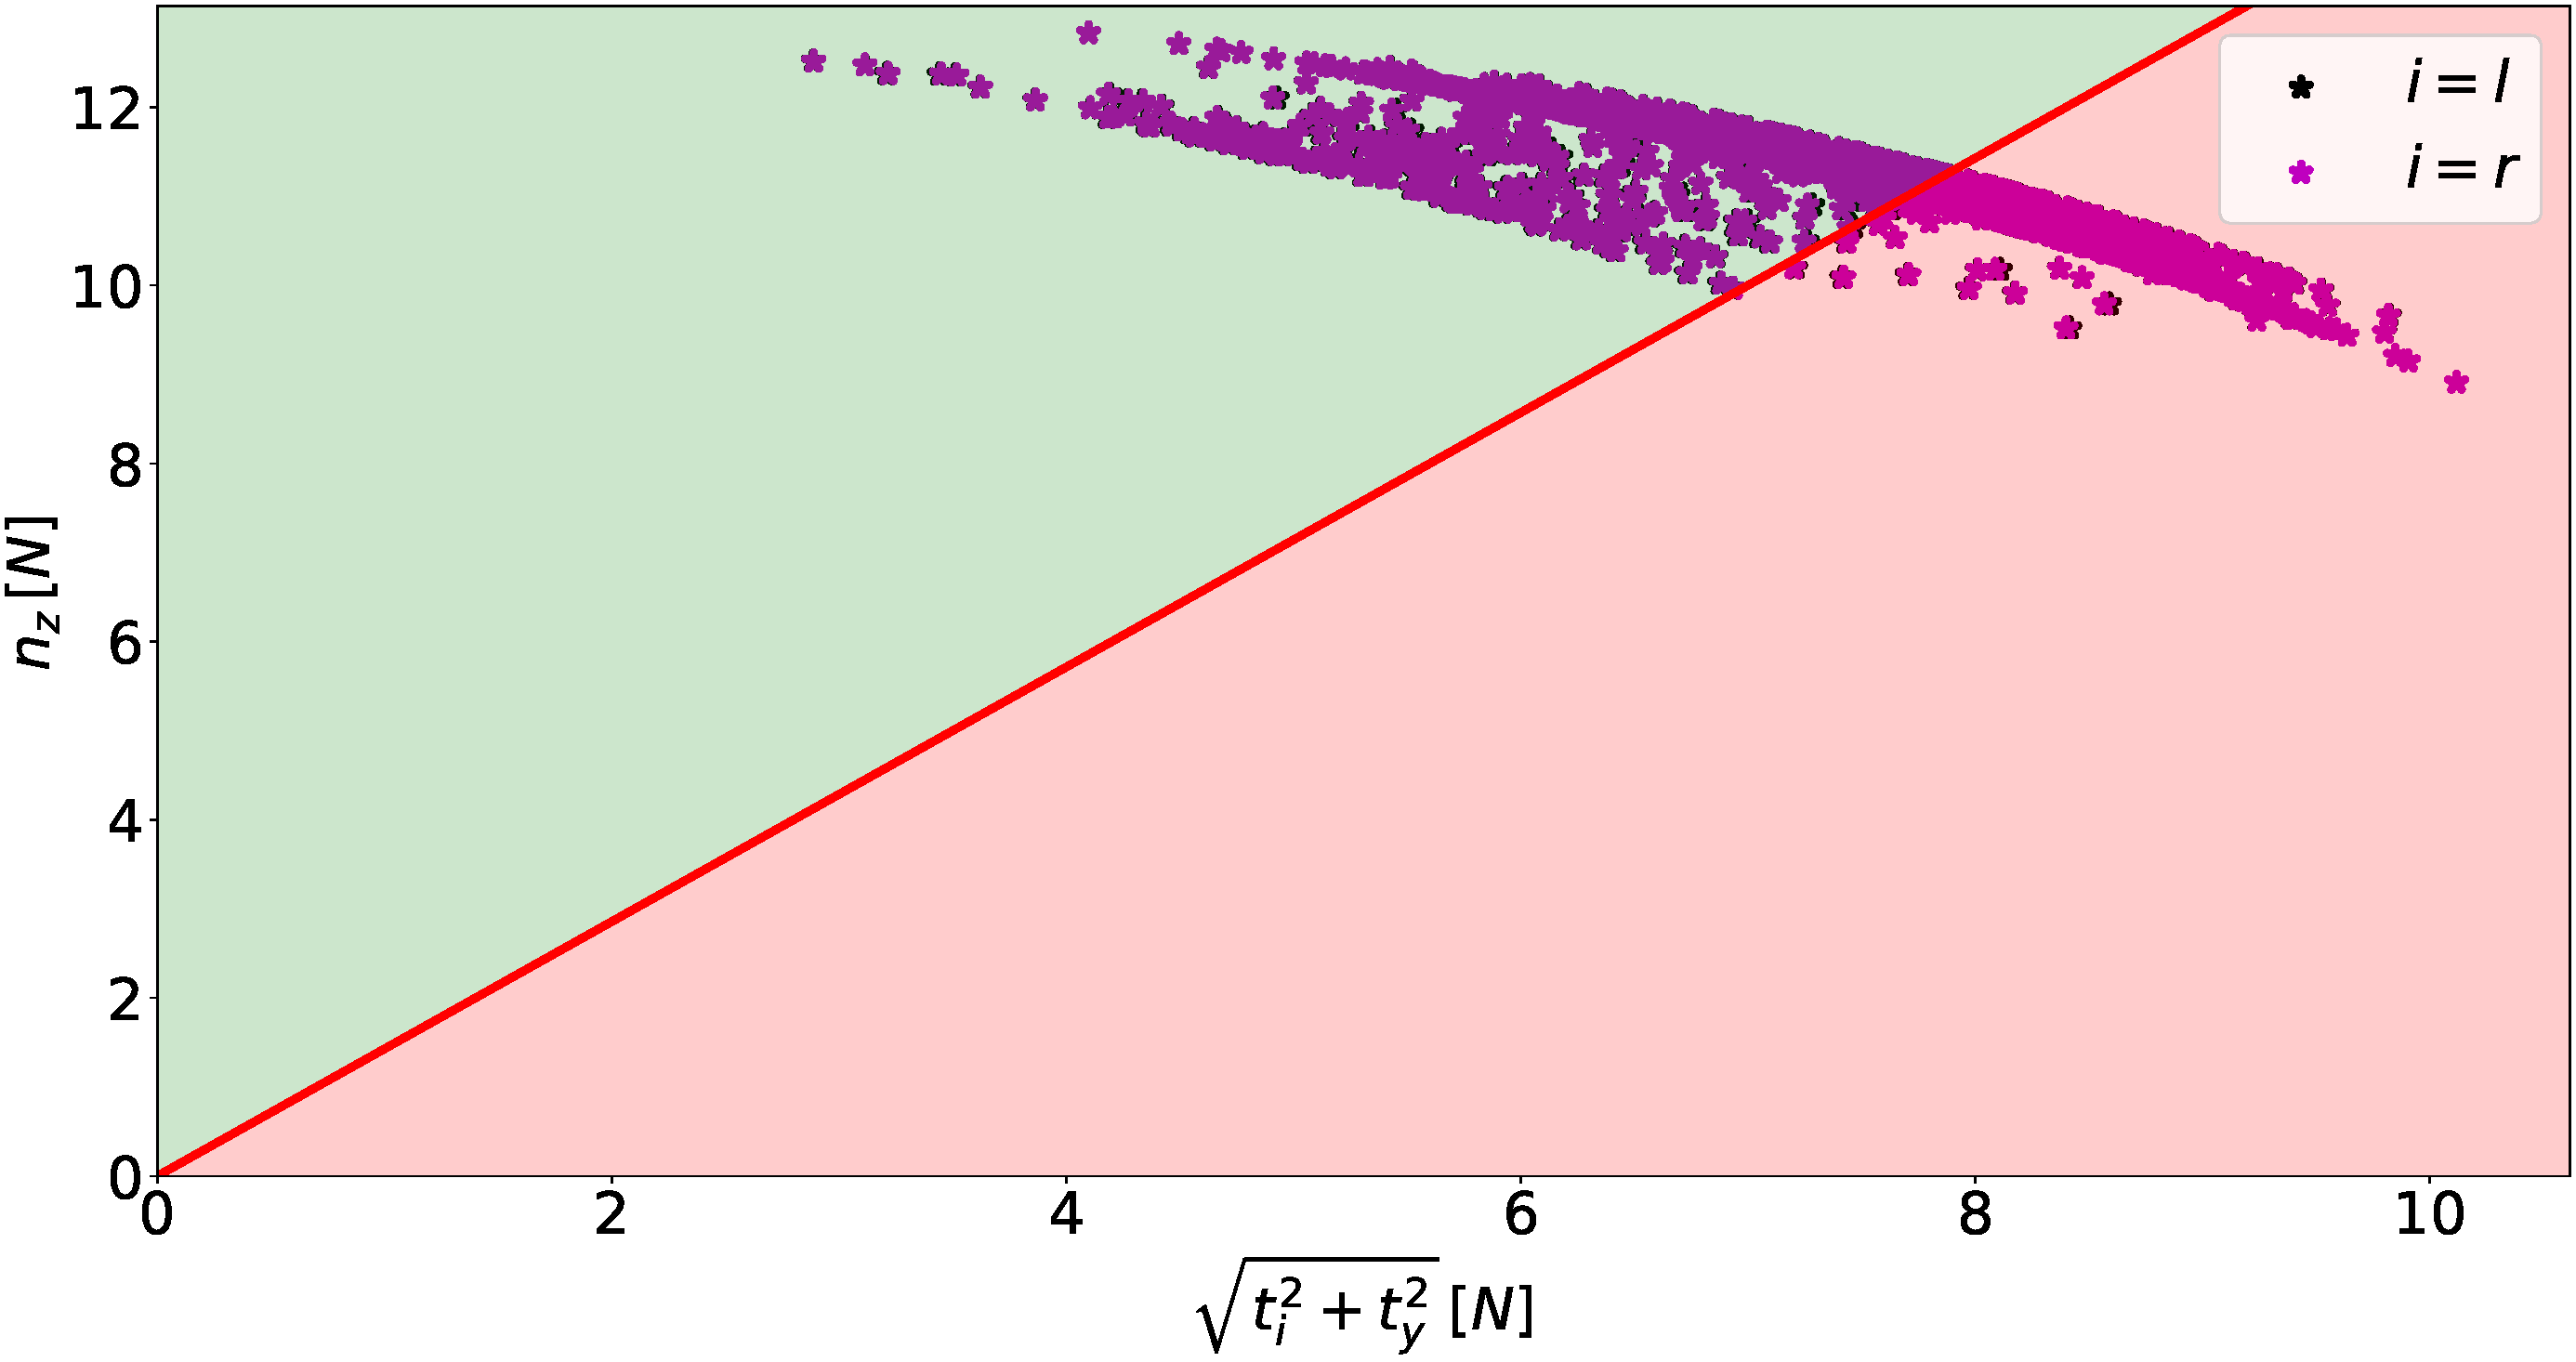
\includegraphics[width=0.31\linewidth]{Figures/Real time one stage OCP on rough terrain/Hill/forces_cone_a_55_2.pdf}}
  \end{subfigmatrix}
  \caption{Coulomb traction forces cone. No slippage area is on \textcolor{tabgreen}{light green} and the slippage area is on \textcolor{tabred}{light red}.}
  \label{fig:ForcesConeHill}
\end{figure}

In case the mobile robot is at some configuration (see subsection \ref{subsection:maxinclination}) where the steady-state traction force is close to the Coulomb friction cone border (red line), there is little room to increase the longitudinal traction force if necessary, which may lead to slippage (and unsafety) as well as solver failure, because the solver tries to look for an optimal solution outside the Coulomb friction cone. The left picture of figure \ref{fig:ForcesConeHill} denotes the recorded optimal wheel traction forces on a scenario of lower steepness, whereas the remaining pictures concern a scenario of higher steepness. As expected, no slippage is recorded when $a=0.33$, although that is not the case when $a=0.55$. 

If one takes the simulation specs of this subsection and sets $\roll = 0,\,\mu = 1$ (therefore $\pitch$ takes the maximum value), \refeq{eq:ForcesRest} yields $0.55^2 \leq 0.7^2$ and $0.33^2 \leq 0.7^2$, when $a=0.55$ and $a=0.33$, respectively, which explains why the mobile robot is more exposed to slippage when $a=0.55$.

Finally, table \ref{tab:hillSolverPerformance} presents the performance results of the solver for the simulations presented in this subsection. As stepness increases, solver times increase a bit. However, timeouts are very rare in all simulations, so the solver is computationally feasible for real-time use. Unsurprisingly, the solver fails the most when the optimal forces are located at the slippage area of the Coulomb friction cone. Solver \ti{Energy saver} attemped to decrease slippage events by keeping the wheel traction force away from the Coulomb friction cone border, but this has not succedded, because the need to track the reference and to provide the respective forces to achieve this goal, govern the entire control simulation.

\begin{remark}
Slippage may also be avoided by feeding the solver with a reference that does not ask for high accelerations, and not just by avoiding spots with high inclinations. In this thesis, the reference computation is controlled by its virtual speed, but the control of the virtual acceleration may largely decrease slippage situations and enlarge the window of accessible locations.
\end{remark}

\begin{table}[!htb]
  \caption[Solver performance on hilly terrain.]{Solver performance over hill traversal.}
  \label{tab:hillSolverPerformance}
  \renewcommand{\arraystretch}{1.2}
  \centering
  \begin{tabular}[]{lccccc}
	\toprule
	& Loop time [ms] & Solver time [ms] & Cost $\times\,[\mathrm{e}{-3}]$ & Timeouts [\%] & \shortstack{Solver fails\\/slippage [\%]} \\
	\midrule
	\textit{Pose tracker} & & & & & \\
	$a=0.33$ & $(5.09) \pm (1.90)$ & $(1.38) \pm (0.17)$ & $(3.82) \pm (14.75)$ & $0.06$ & $0.0$\\
	$a=0.55$ & $(4.94) \pm (1.49)$ & $(1.45) \pm (0.47)$ & $(4.46) \pm (17.69)$ & $0.02$ & $83.45$\\
	\textit{Energy saver} & & & & & \\
	$a=0.55$ & $(5.31) \pm (1.50)$ & $(1.60) \pm (0.61)$ & $(6.21) \pm (113.29)$ & $0.4$ & $84.62$\\
  	\bottomrule
  \end{tabular}
\end{table}
\subsection{Traversal of rough, uneven terrain}
\label{subsection:traversalRoughTerrain}

After the first assessment of the \acrshort{nmpc} over a hilly scenario, the performance analysis of the same architecture is carried on for a more complex terrain. This time, the chosen heightmap is of the type $h\left(\x,\,\y\right) = c \, \sin(a\,x) \, \cos(b\,y)$, where $a,\,b,\,c$ denote parameters of the heightmap.

In the virtual speed control module, \refeq{eq:vspeed_computation_architecture_b} is replaced by \eqref{eq:vspeed_computation_architecture_b_2}. The weighted average is still given by \refeq{eq:virtualspeedqp}.

\begin{equation}
v_i\left(\kappa,\,\varepsilon\right) = min\left( \frac{0.1}{ 1 + \exp\left( 5.0\,( \varepsilon - 2.0 ) \right) },\, \frac{0.1}{ 1 + \exp\left( 0.1\,( \kappa - 10.0 ) \right) } \right)
\label{eq:vspeed_computation_architecture_b_2}
\end{equation}

\begin{table}[!htb]
  \caption[Solver parameters on hill.]{Path tracking solver parameters ($N = 50,\; T_s = 20\,ms$).}
  \label{tab:RoughPathTrackingSpecs}
  \renewcommand{\arraystretch}{1.2}
  \centering
  \begin{tabular}[]{lcccccccc}
	\toprule
	& $Q_i$ & $R$\\
	\midrule
	Fast rate of change & $diag\left(3.0\times 1.1^i \cdot \mathbf{1}_3,\,1\mathrm{e}{-9} \cdot \mathbf{1}_4\right)$ & $1\mathrm{e}{-3} \cdot \mathbf{1}_2$\\
	Moderate rate of change & $diag\left(3.0\times 1.1^i \cdot \mathbf{1}_3,\,1\mathrm{e}{-9} \cdot \mathbf{1}_4\right)$ & $1\mathrm{e}{-1} \cdot \mathbf{1}_2$\\
	Low rate of change & $diag\left(3.0\times 1.1^i \cdot \mathbf{1}_3,\,1\mathrm{e}{-9} \cdot \mathbf{1}_4\right)$ & $\mathbf{1}_2$\\
	Energy saver & $diag\left(3.0\times 1.1^i \cdot \mathbf{1}_3,\,1\mathrm{e}{-9} \cdot \mathbf{1}_2,\,1\mathrm{e}{-4} \cdot \mathbf{1}_2\right)$ & $\mathbf{1}_2$\\
	Very low rate of change & $diag\left(3.0\times 1.1^i \cdot \mathbf{1}_3,\,1\mathrm{e}{-9} \cdot \mathbf{1}_2,\,1\mathrm{e}{-4} \cdot \mathbf{1}_2\right)$ & $2.0 \cdot \mathbf{1}_2$\\
	\end{tabular}
	\begin{tabular}[]{cccccc}
  	\toprule
  		$\left[(v_x)_{min},\; (v_x)_{max}\right]\,[m/s]$ & $\left[(\omega_z)_{min},\; (\omega_z)_{max}\right]\,[rad/s]$ & $\left[(u_i)_{min},\,(u_i)_{max}\right]\,[N \cdot s]$ & $\FrictionCoefficient$ & $\sigma_{\roll}$ & $\sigma_{\pitch}$\\
  	\midrule
  		$\left[-5.0,\,5.0\right]$ & $\left[-5.0,\,5.0\right]$ & $\left[-100,\,100\right]$ & $0.7$ & $7\mathrm{e}{-2}$ & $7\mathrm{e}{-2}$\\
  	\bottomrule
  \end{tabular}
\end{table}

Figure \ref{fig:pathCompRoughTerrain} presents the first 1500 iterations of path tracking control with the solvers of table \ref{tab:RoughPathTrackingSpecs}, in order to survey the controller reaction to a situation where the initial yaw is $\pi\,[rad]$ deviated from the reference yaw. Apart from solver \ti{Fast rate of change}, the controllers successfully guide the mobile robot along the reference with the correct heading. Picture \ref{subfig:rollpitchref2} denotes an example of the roll and pitch fluctuation for the chosen heightmap.

Figure \ref{fig:RoughUnevenTerrainForcesConeHill} depicts the set of optimal wheel traction forces generated by the solvers of table \ref{tab:RoughPathTrackingSpecs}. Slippage is not avoided by placing higher weights on $\delta \Traction_i$, but rather on $u_i$. Higher forces were achieved in the beginning of the simulation when the solver is asked to address a greater heading error. Although it is normal for the solver to generate higher wheel traction forces in these situations, greater forces are recorded if big spikes on the forces are allowed. Then, the solver response to pose errors needs to be restrained so that the wheel traction forces rate of change decreases. Figure \ref{fig:Forces_ForcesRates_Curves} shows evidence of what is described in this paragraph. Equation \eqref{eq:forcesLimits} outlines the limits of the traction deviations. These limits are determined by replacing \refeq{eq:reformSumForces} into \eqref{eq:skidsteeringcoulomb} and by solving the respective equation with respect to $\delta\Traction_i$. Picture \ref{subfig:traction_rates_solvers_2_4} shows the effect of placing higher weights in the traction rates.

\begin{figure}[!htb]
  \begin{subfigmatrix}{2}
    \subfigure[Path tracking on rough, uneven terrain.]{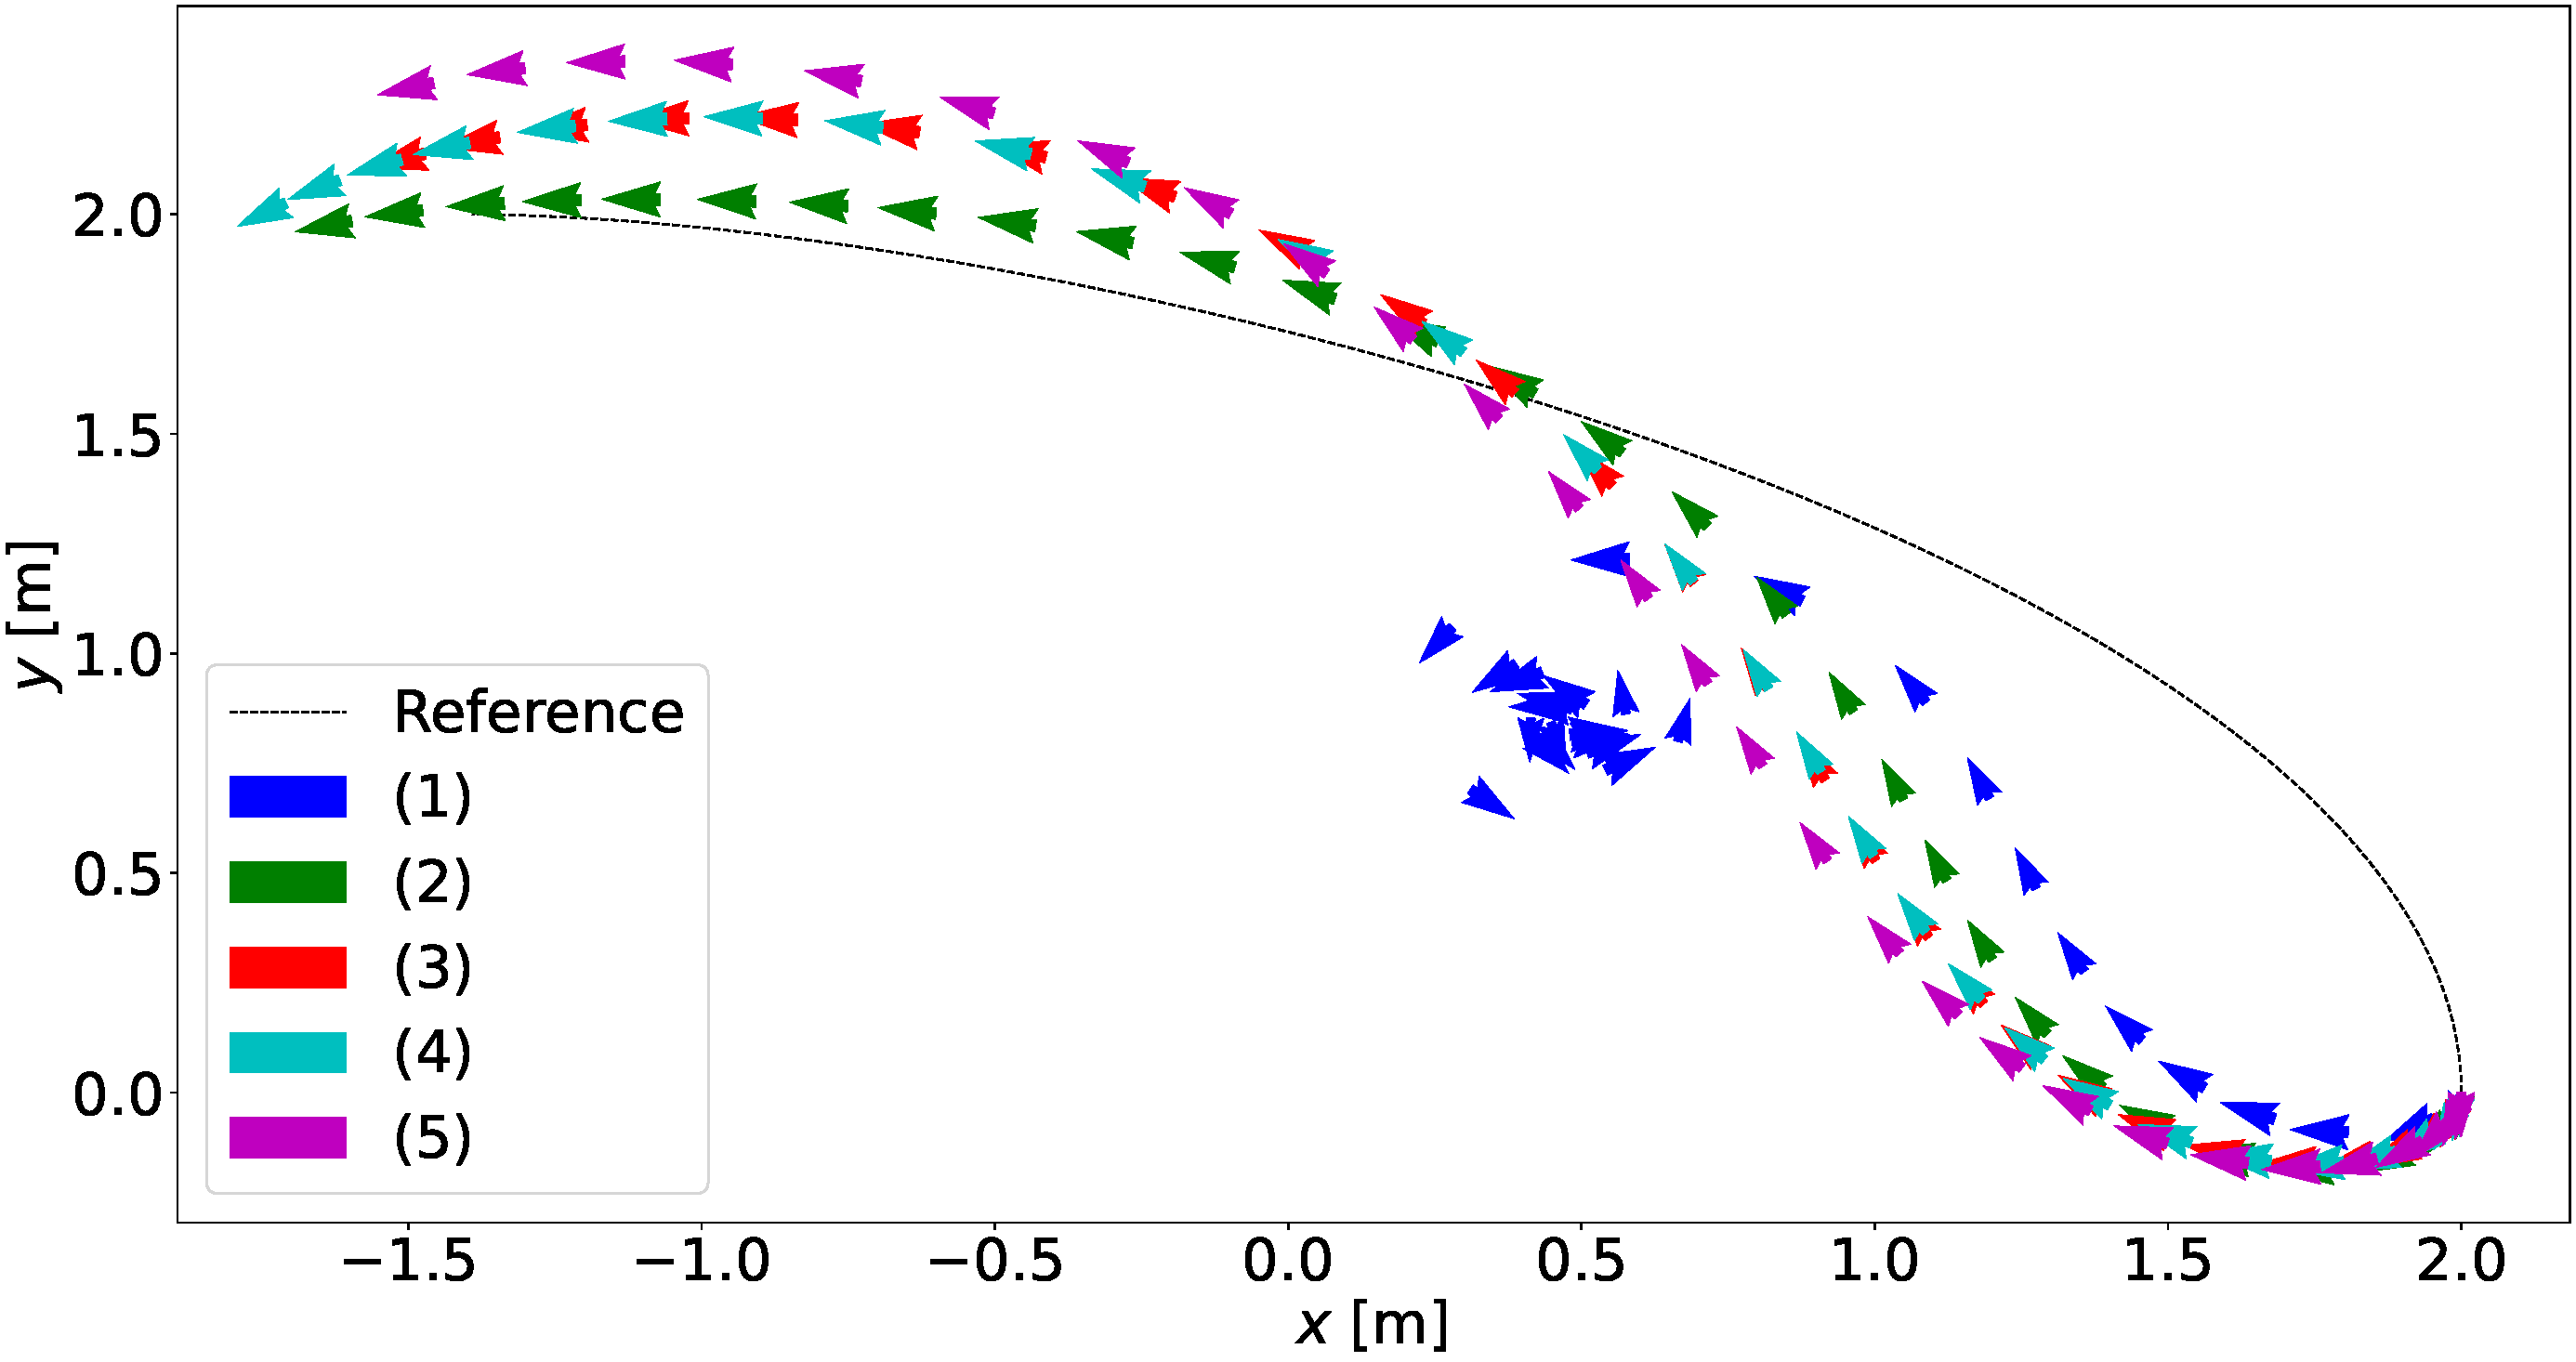
\includegraphics[width=0.49\linewidth]{Figures/Real time one stage OCP on rough terrain/Rough and uneven terrain map/Path_comparison.pdf}}
    \subfigure[Example of pitch \textcolor{orange}{(orange)} and roll \textcolor{blue}{(blue)} fluctuation.]{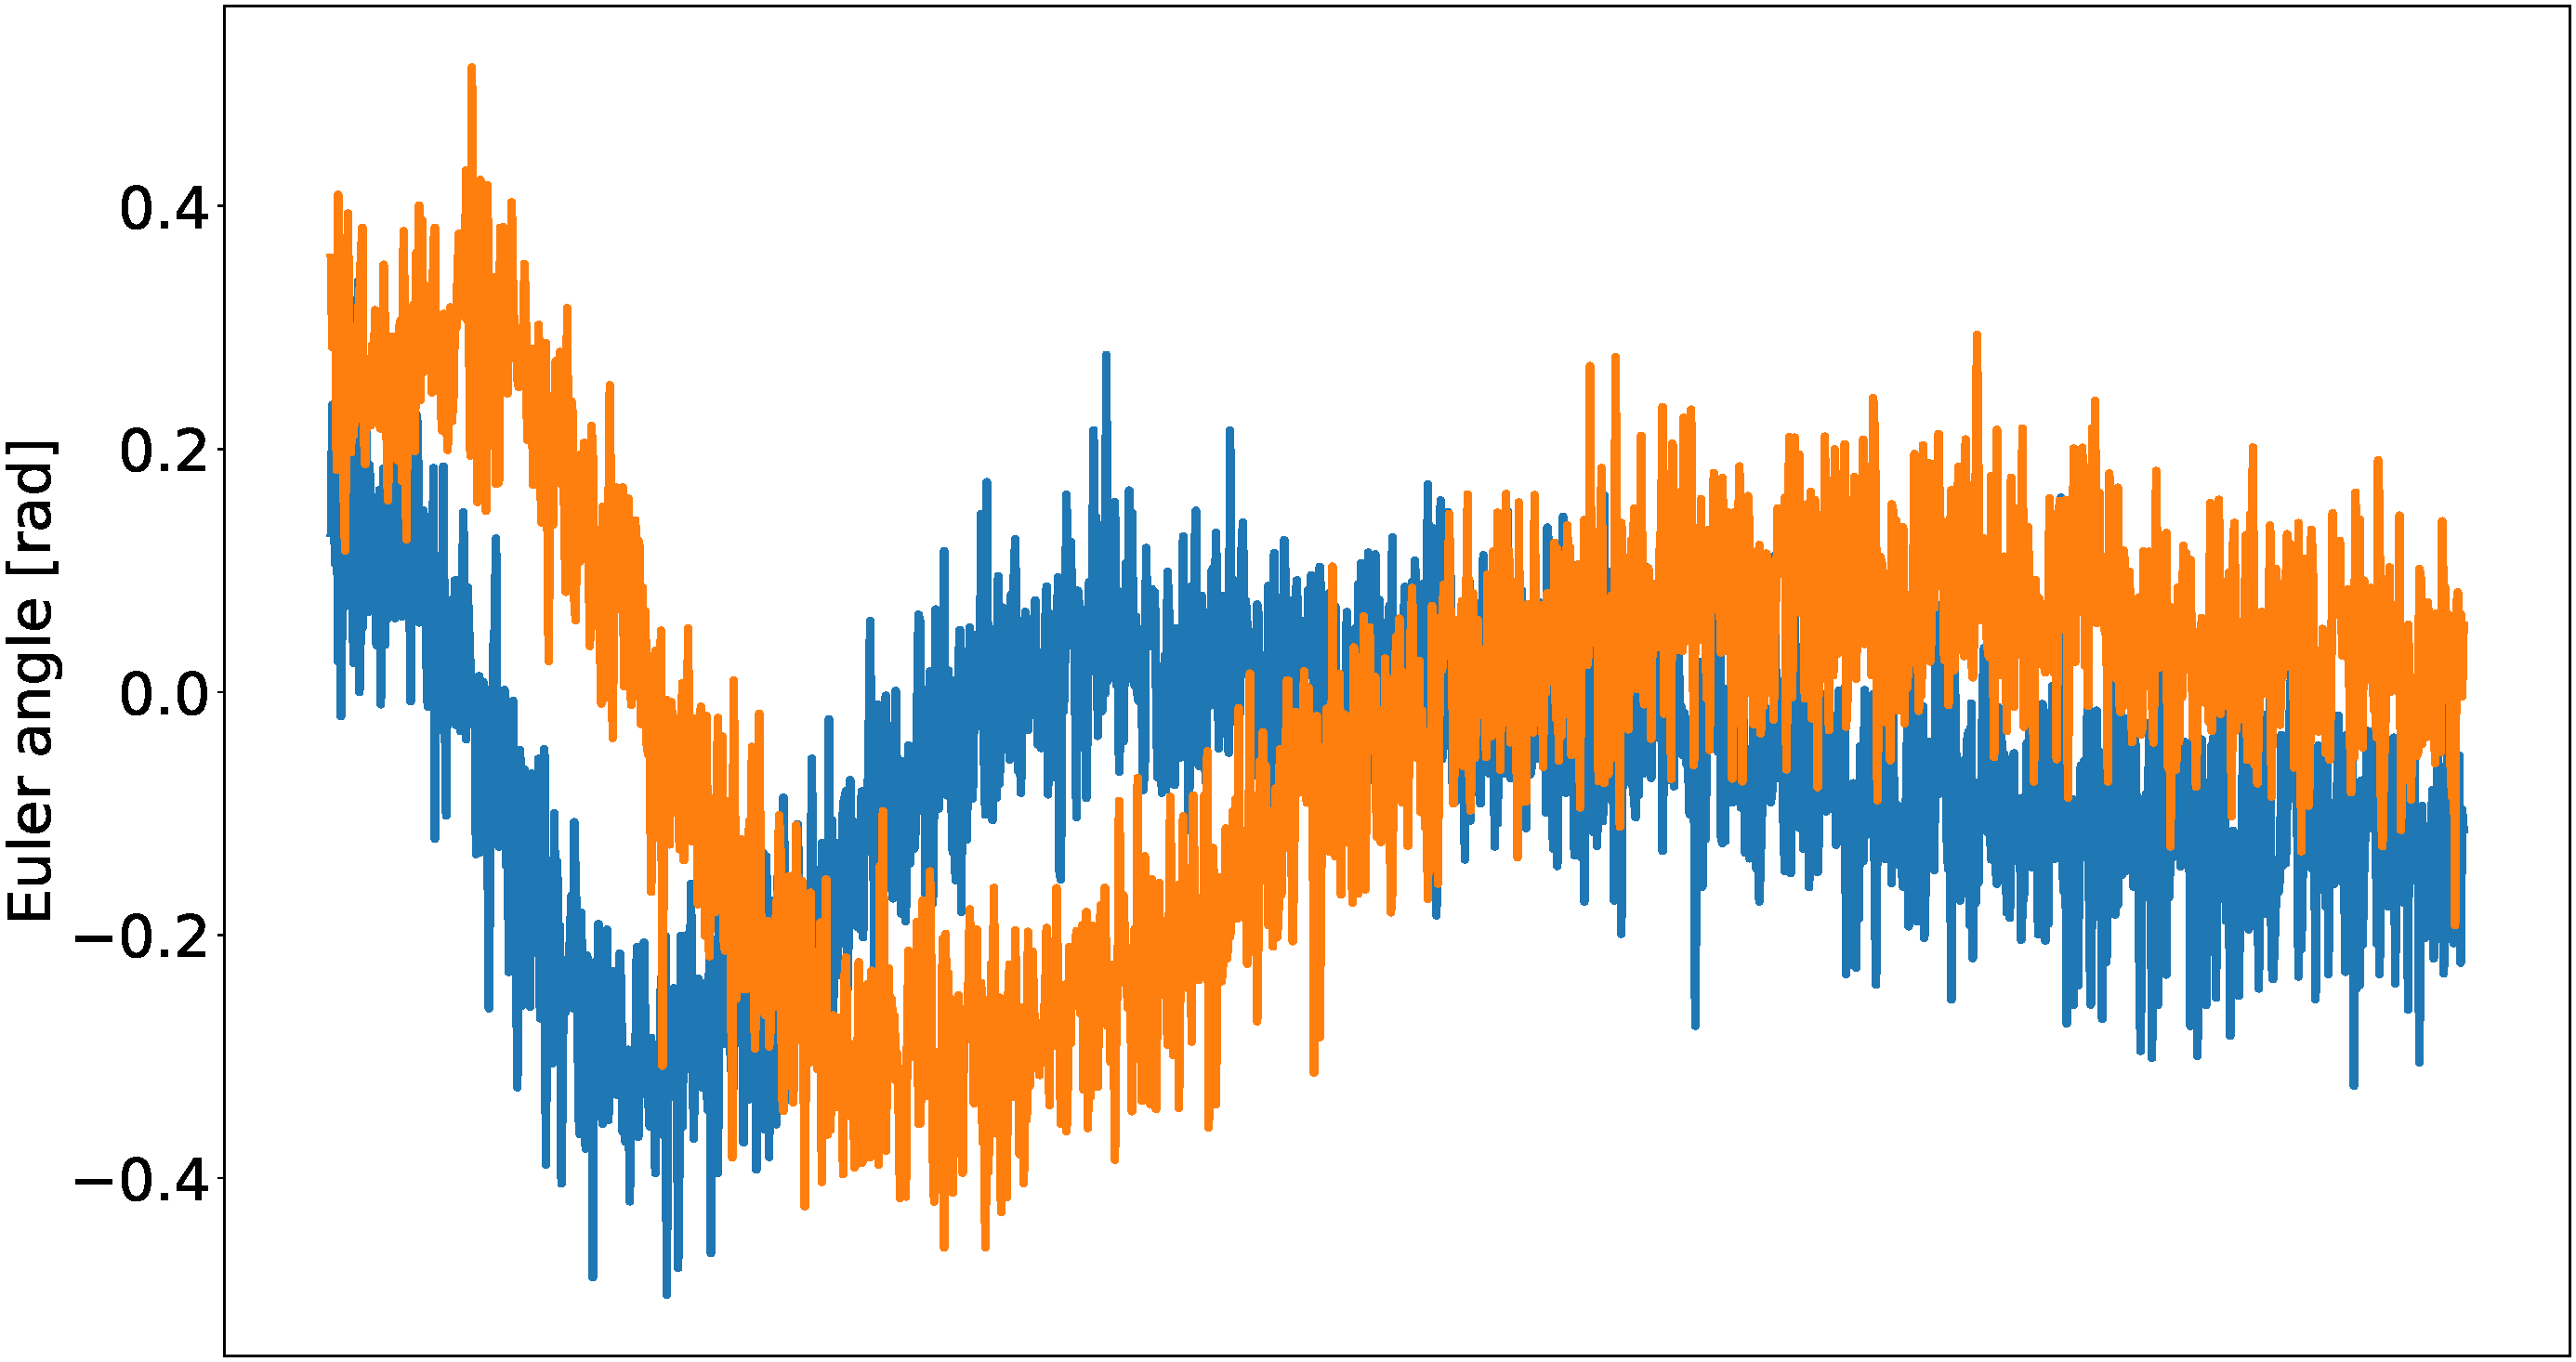
\includegraphics[width=0.49\linewidth]{Figures/Real time one stage OCP on rough terrain/Rough and uneven terrain map/roll_and_pitch.pdf}
    \label{subfig:rollpitchref2}}
  \end{subfigmatrix}
  \caption{Initial path tracking on rough, uneven terrain, where $a=1.0,\,b=1.0,\,c=0.3$.}
  \label{fig:pathCompRoughTerrain}
\end{figure}

\begin{figure}[!htb]
  \begin{subfigmatrix}{3}
    \subfigure[Fast rate of change.]{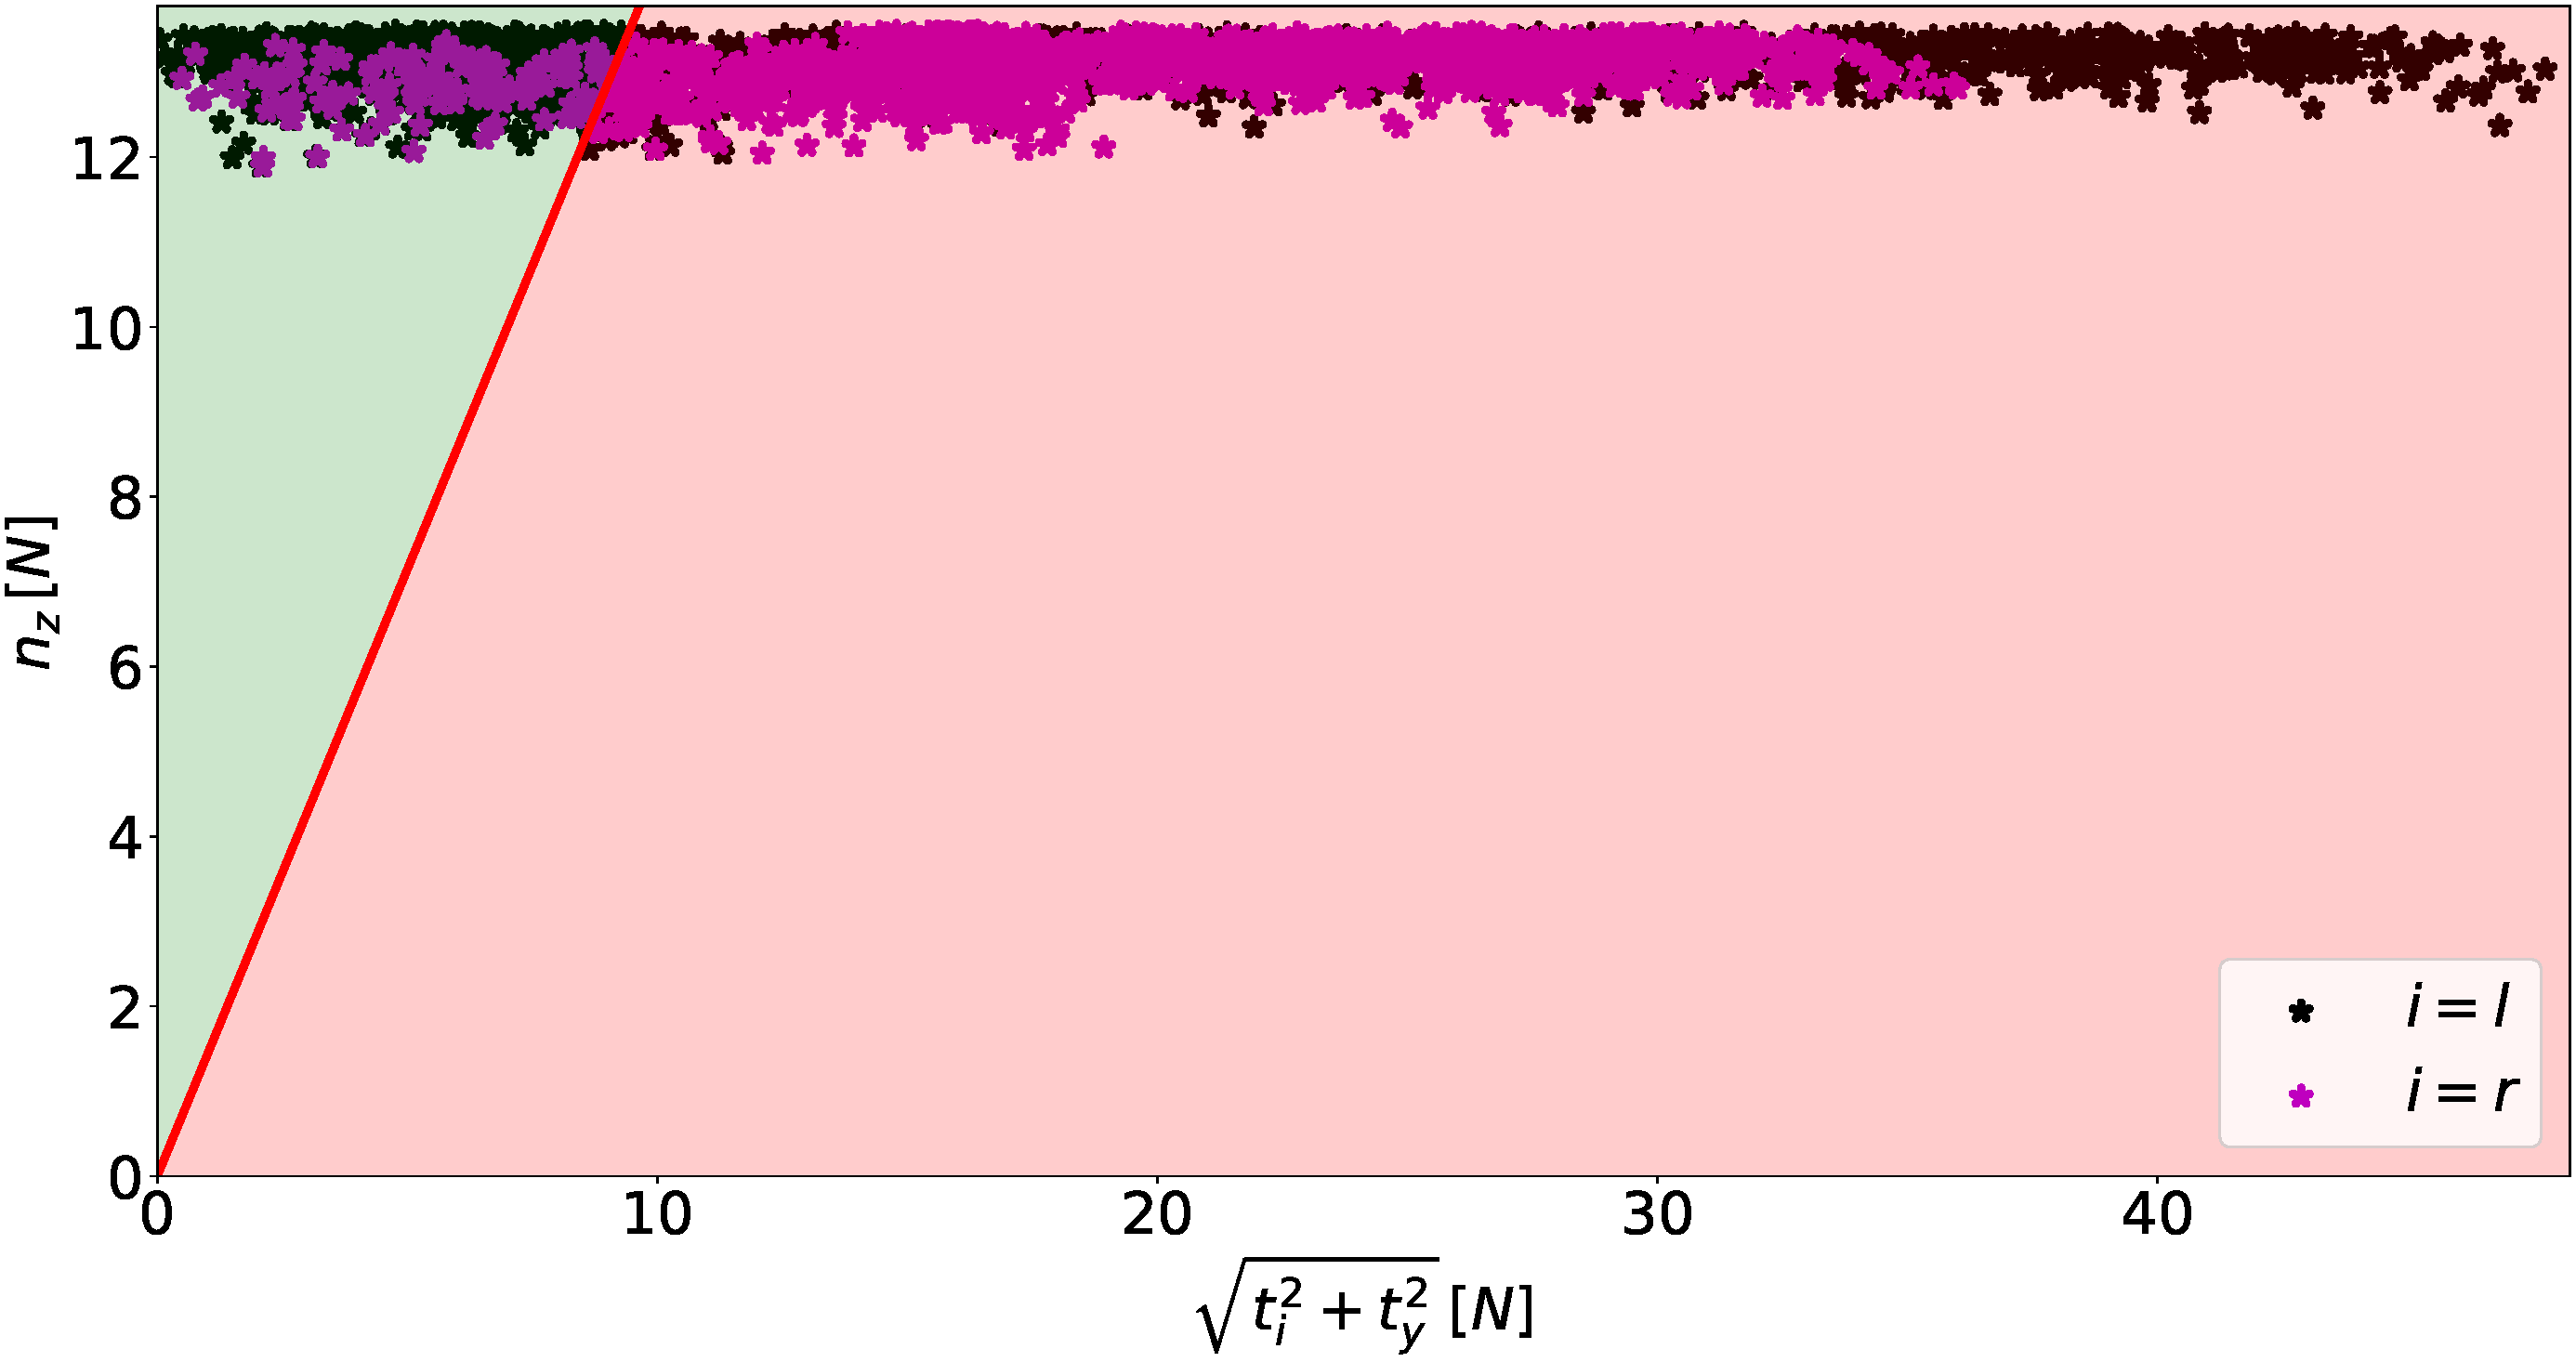
\includegraphics[width=0.325\linewidth]{Figures/Real time one stage OCP on rough terrain/Rough and uneven terrain map/forces_cone_1.pdf}}
    \subfigure[Moderate rate of change.]{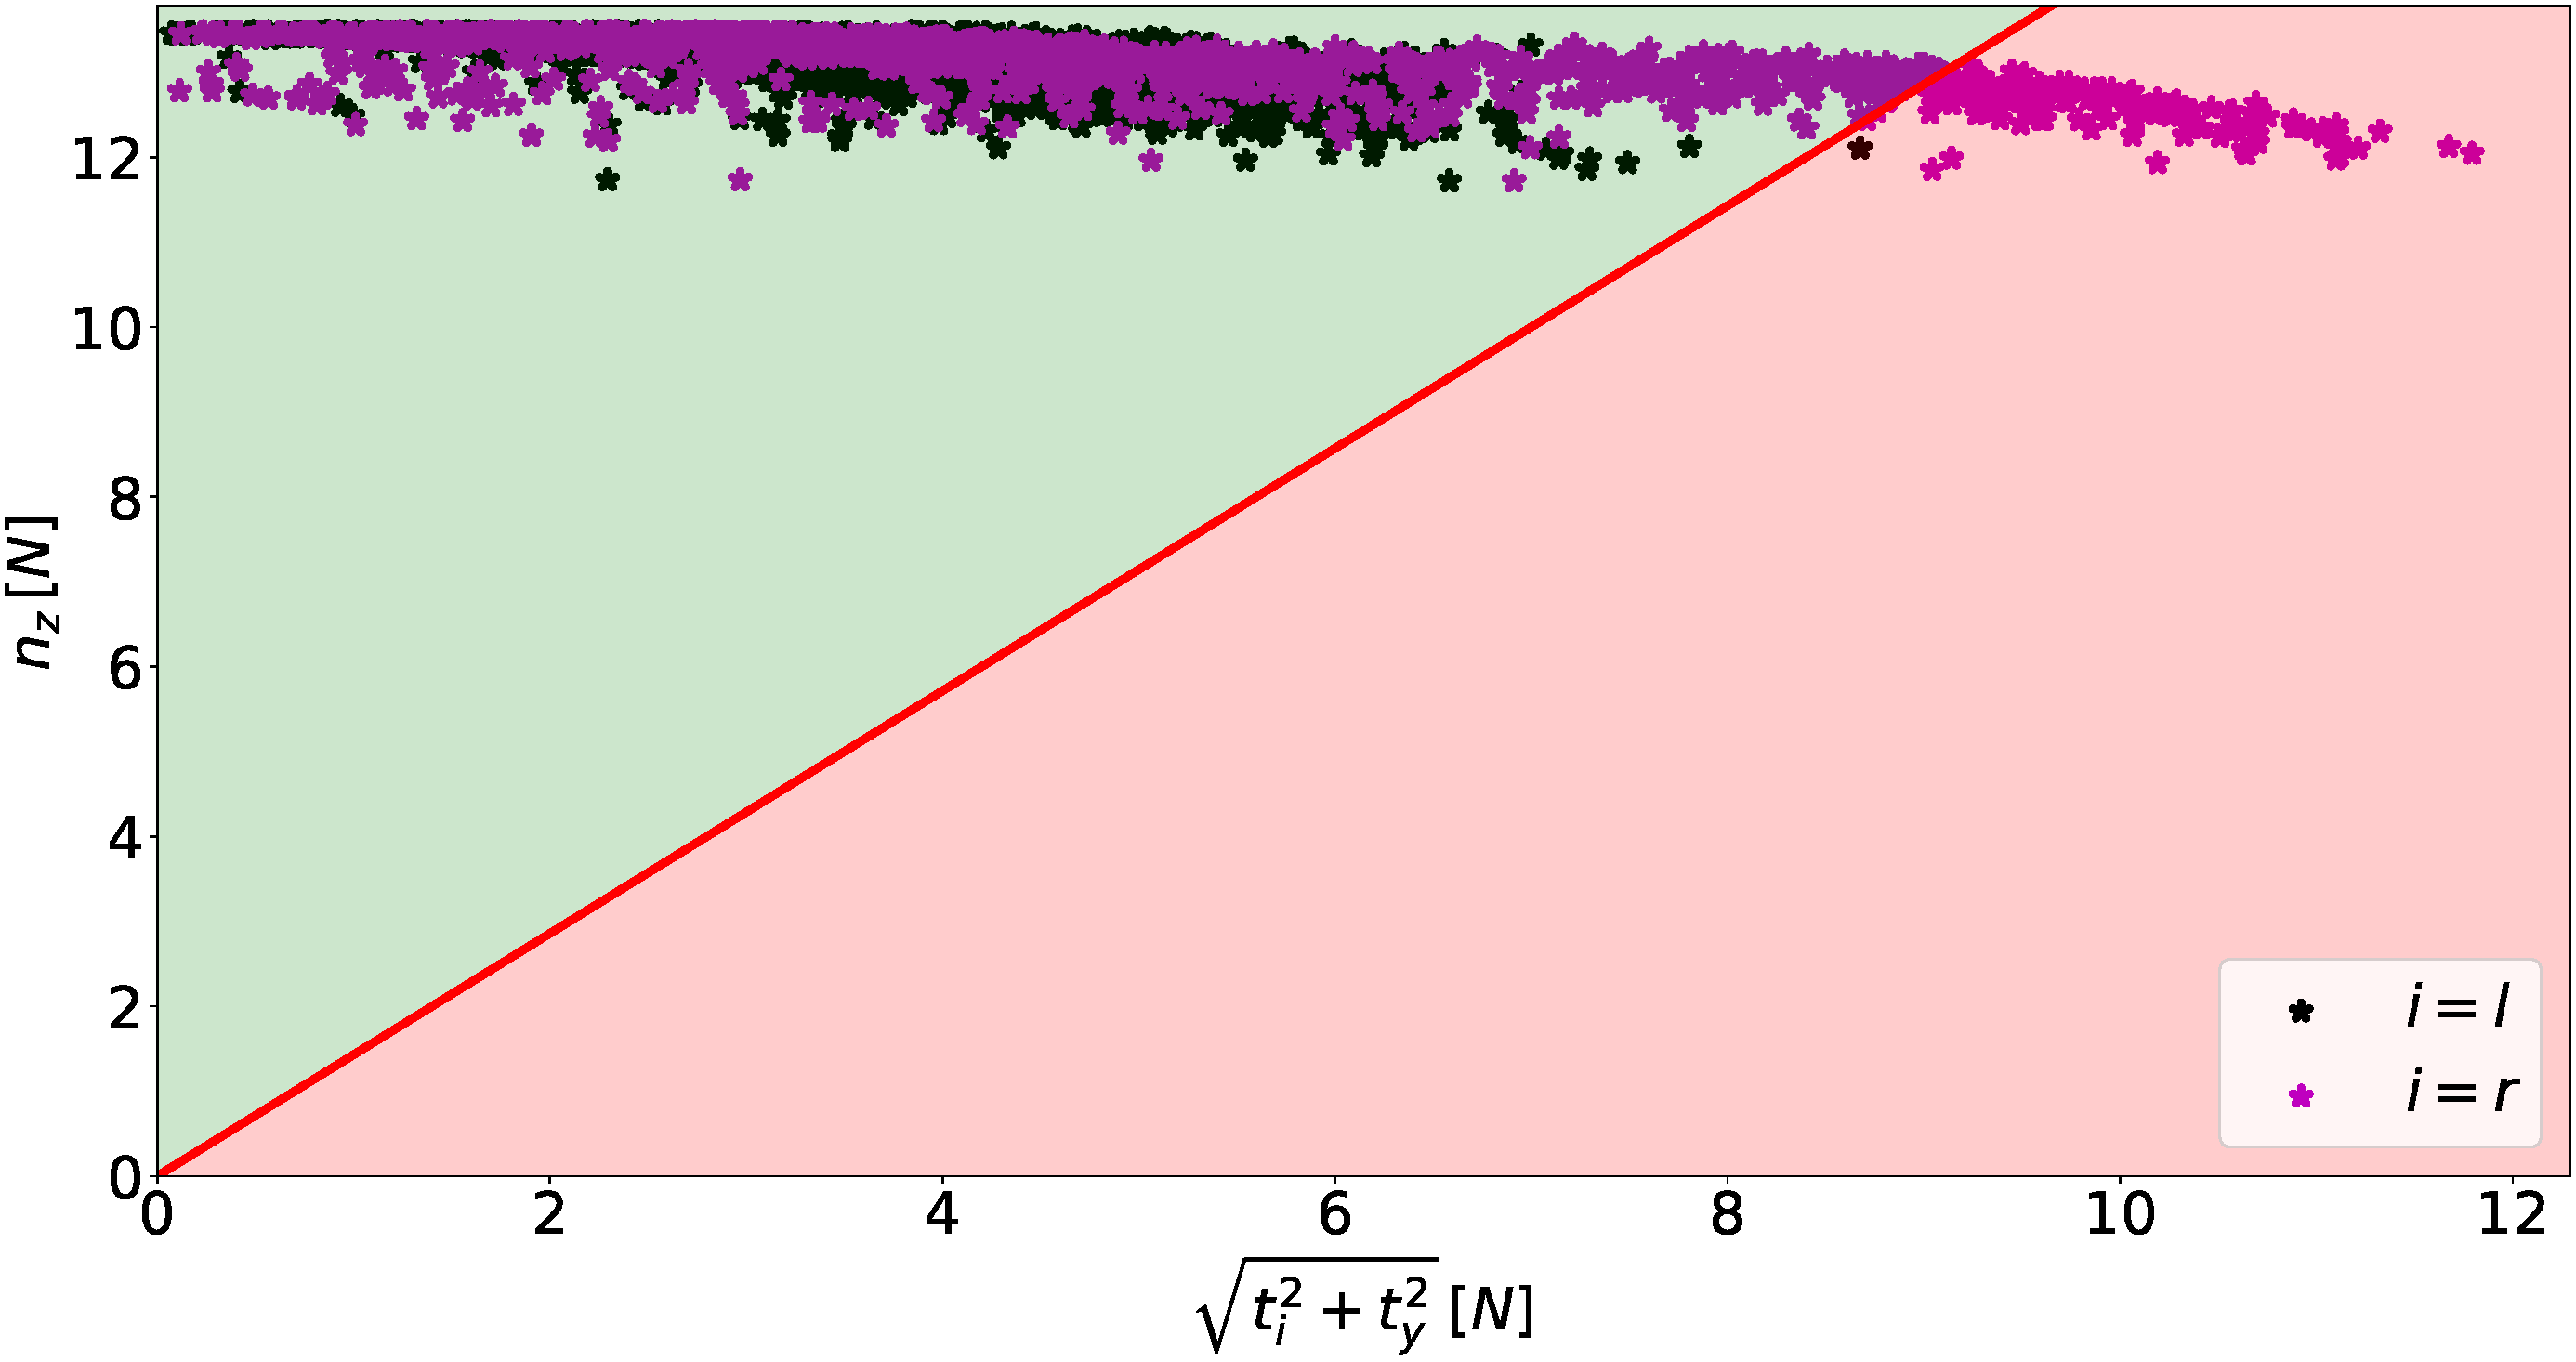
\includegraphics[width=0.325\linewidth]{Figures/Real time one stage OCP on rough terrain/Rough and uneven terrain map/forces_cone_2.pdf}}
    \subfigure[Low rate of change.]{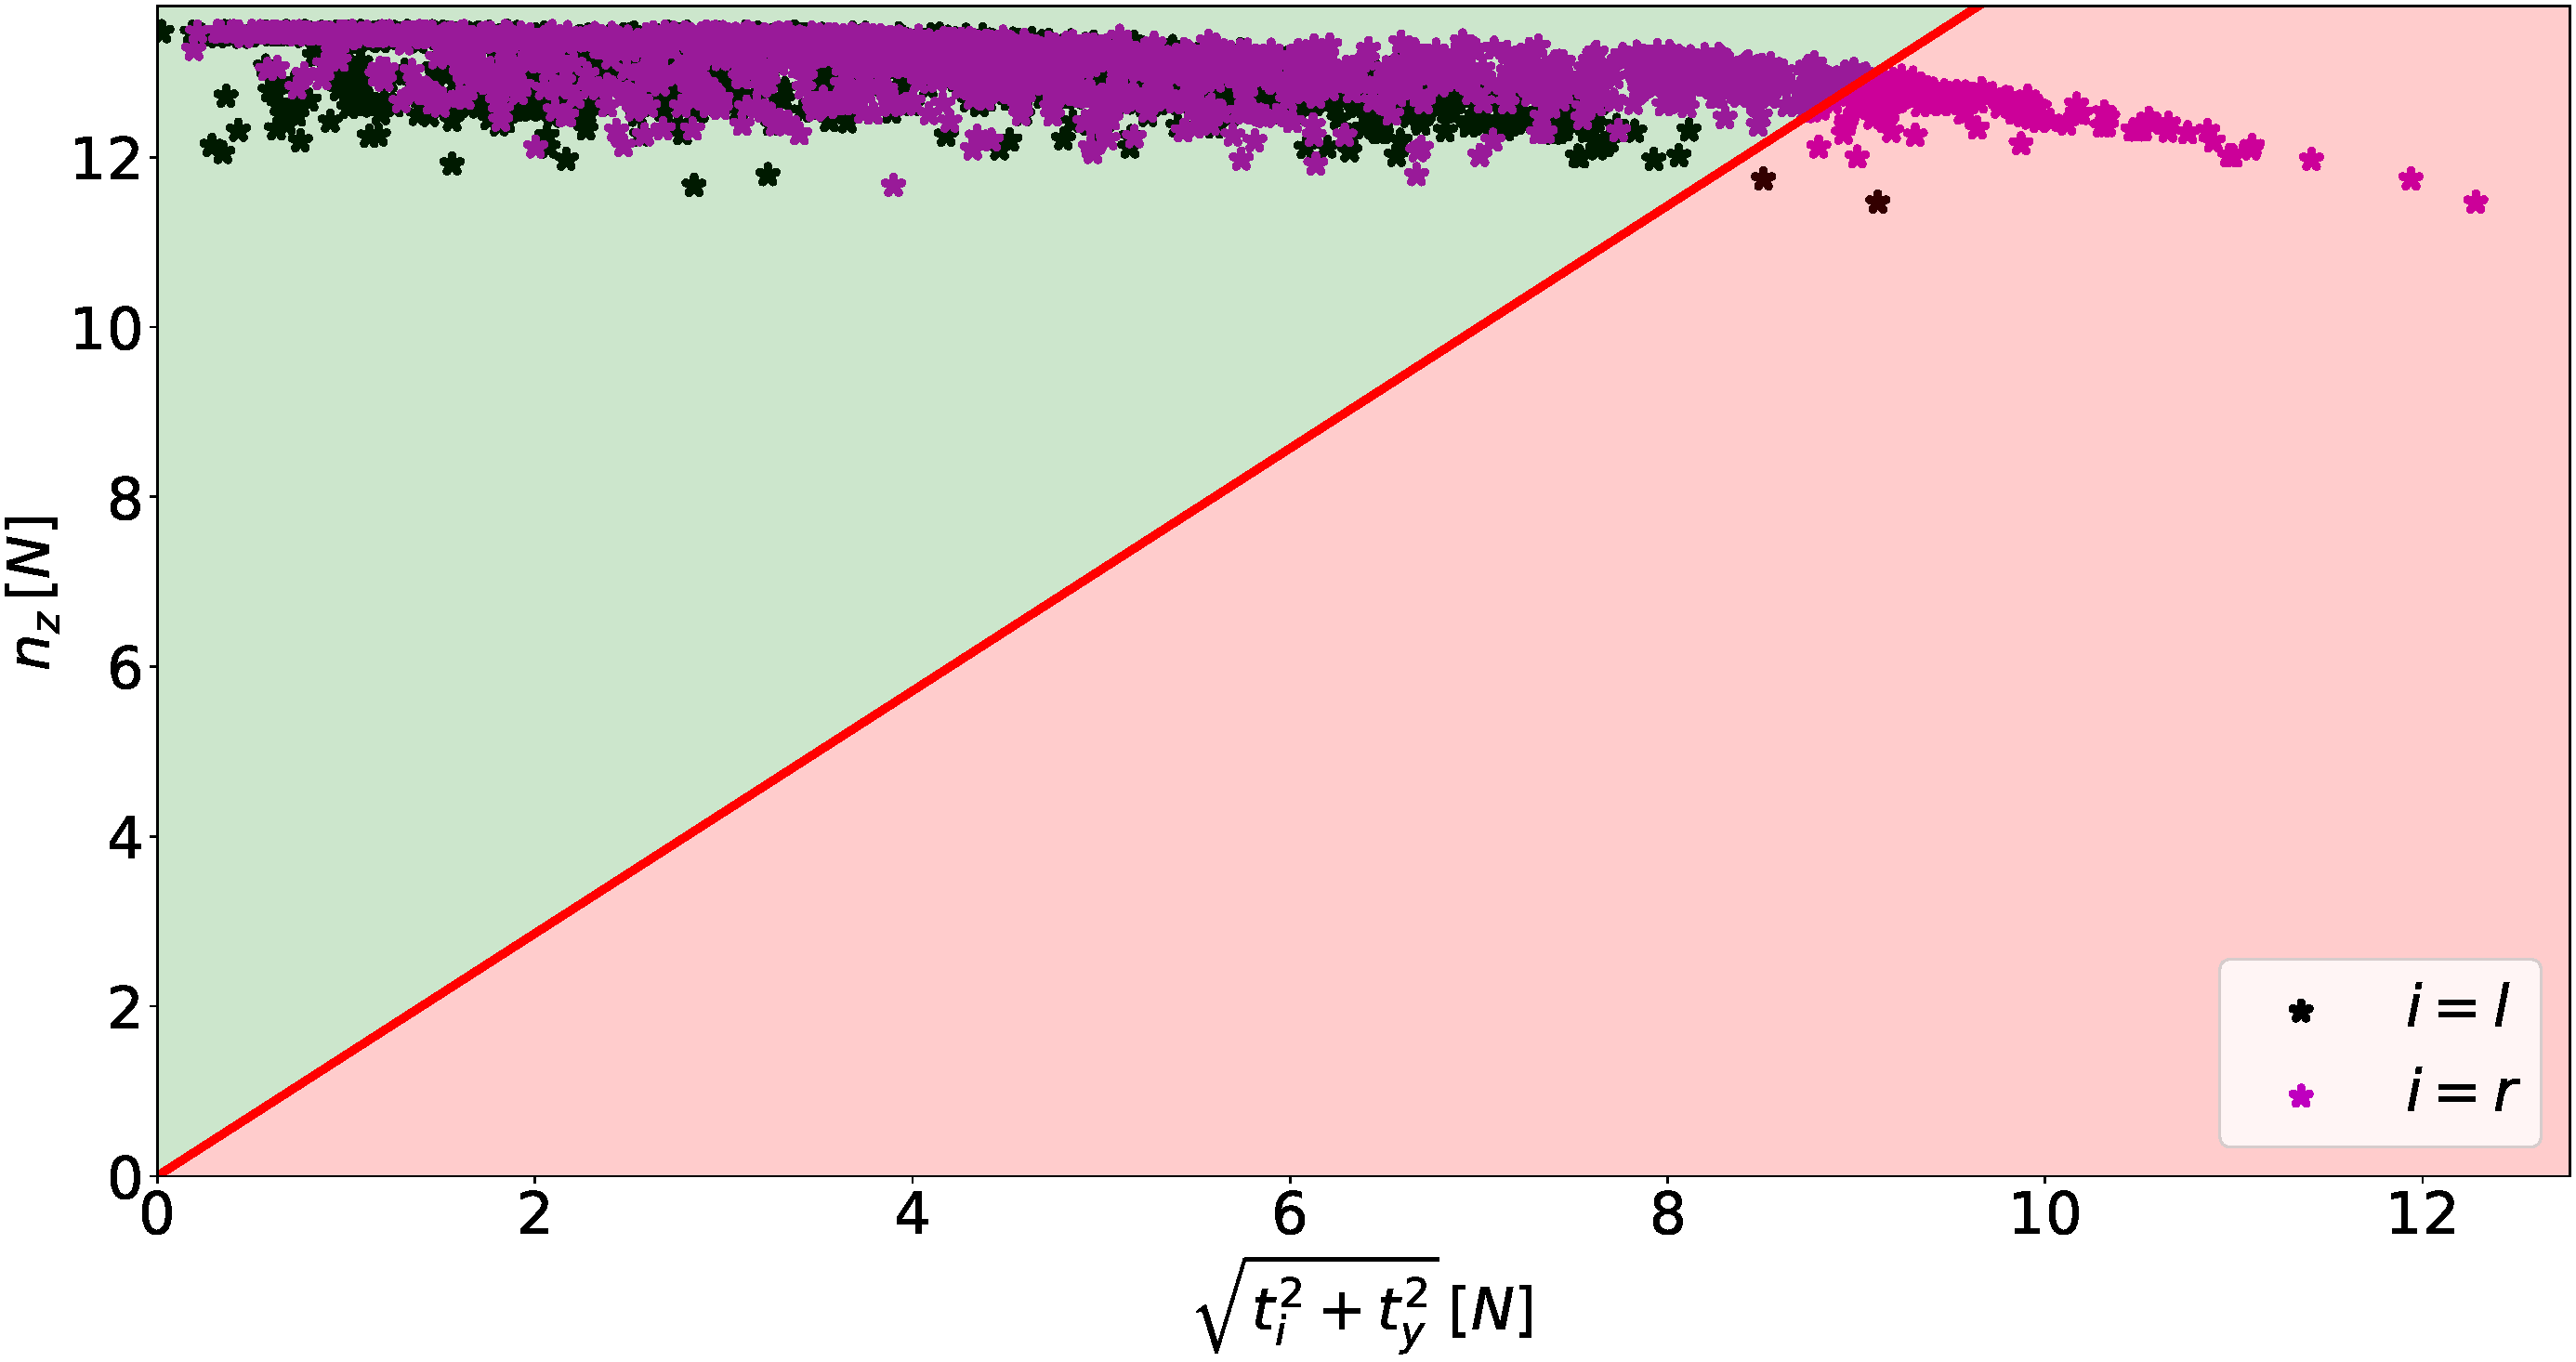
\includegraphics[width=0.325\linewidth]{Figures/Real time one stage OCP on rough terrain/Rough and uneven terrain map/forces_cone_3.pdf}}
    \subfigure[Energy saver.]{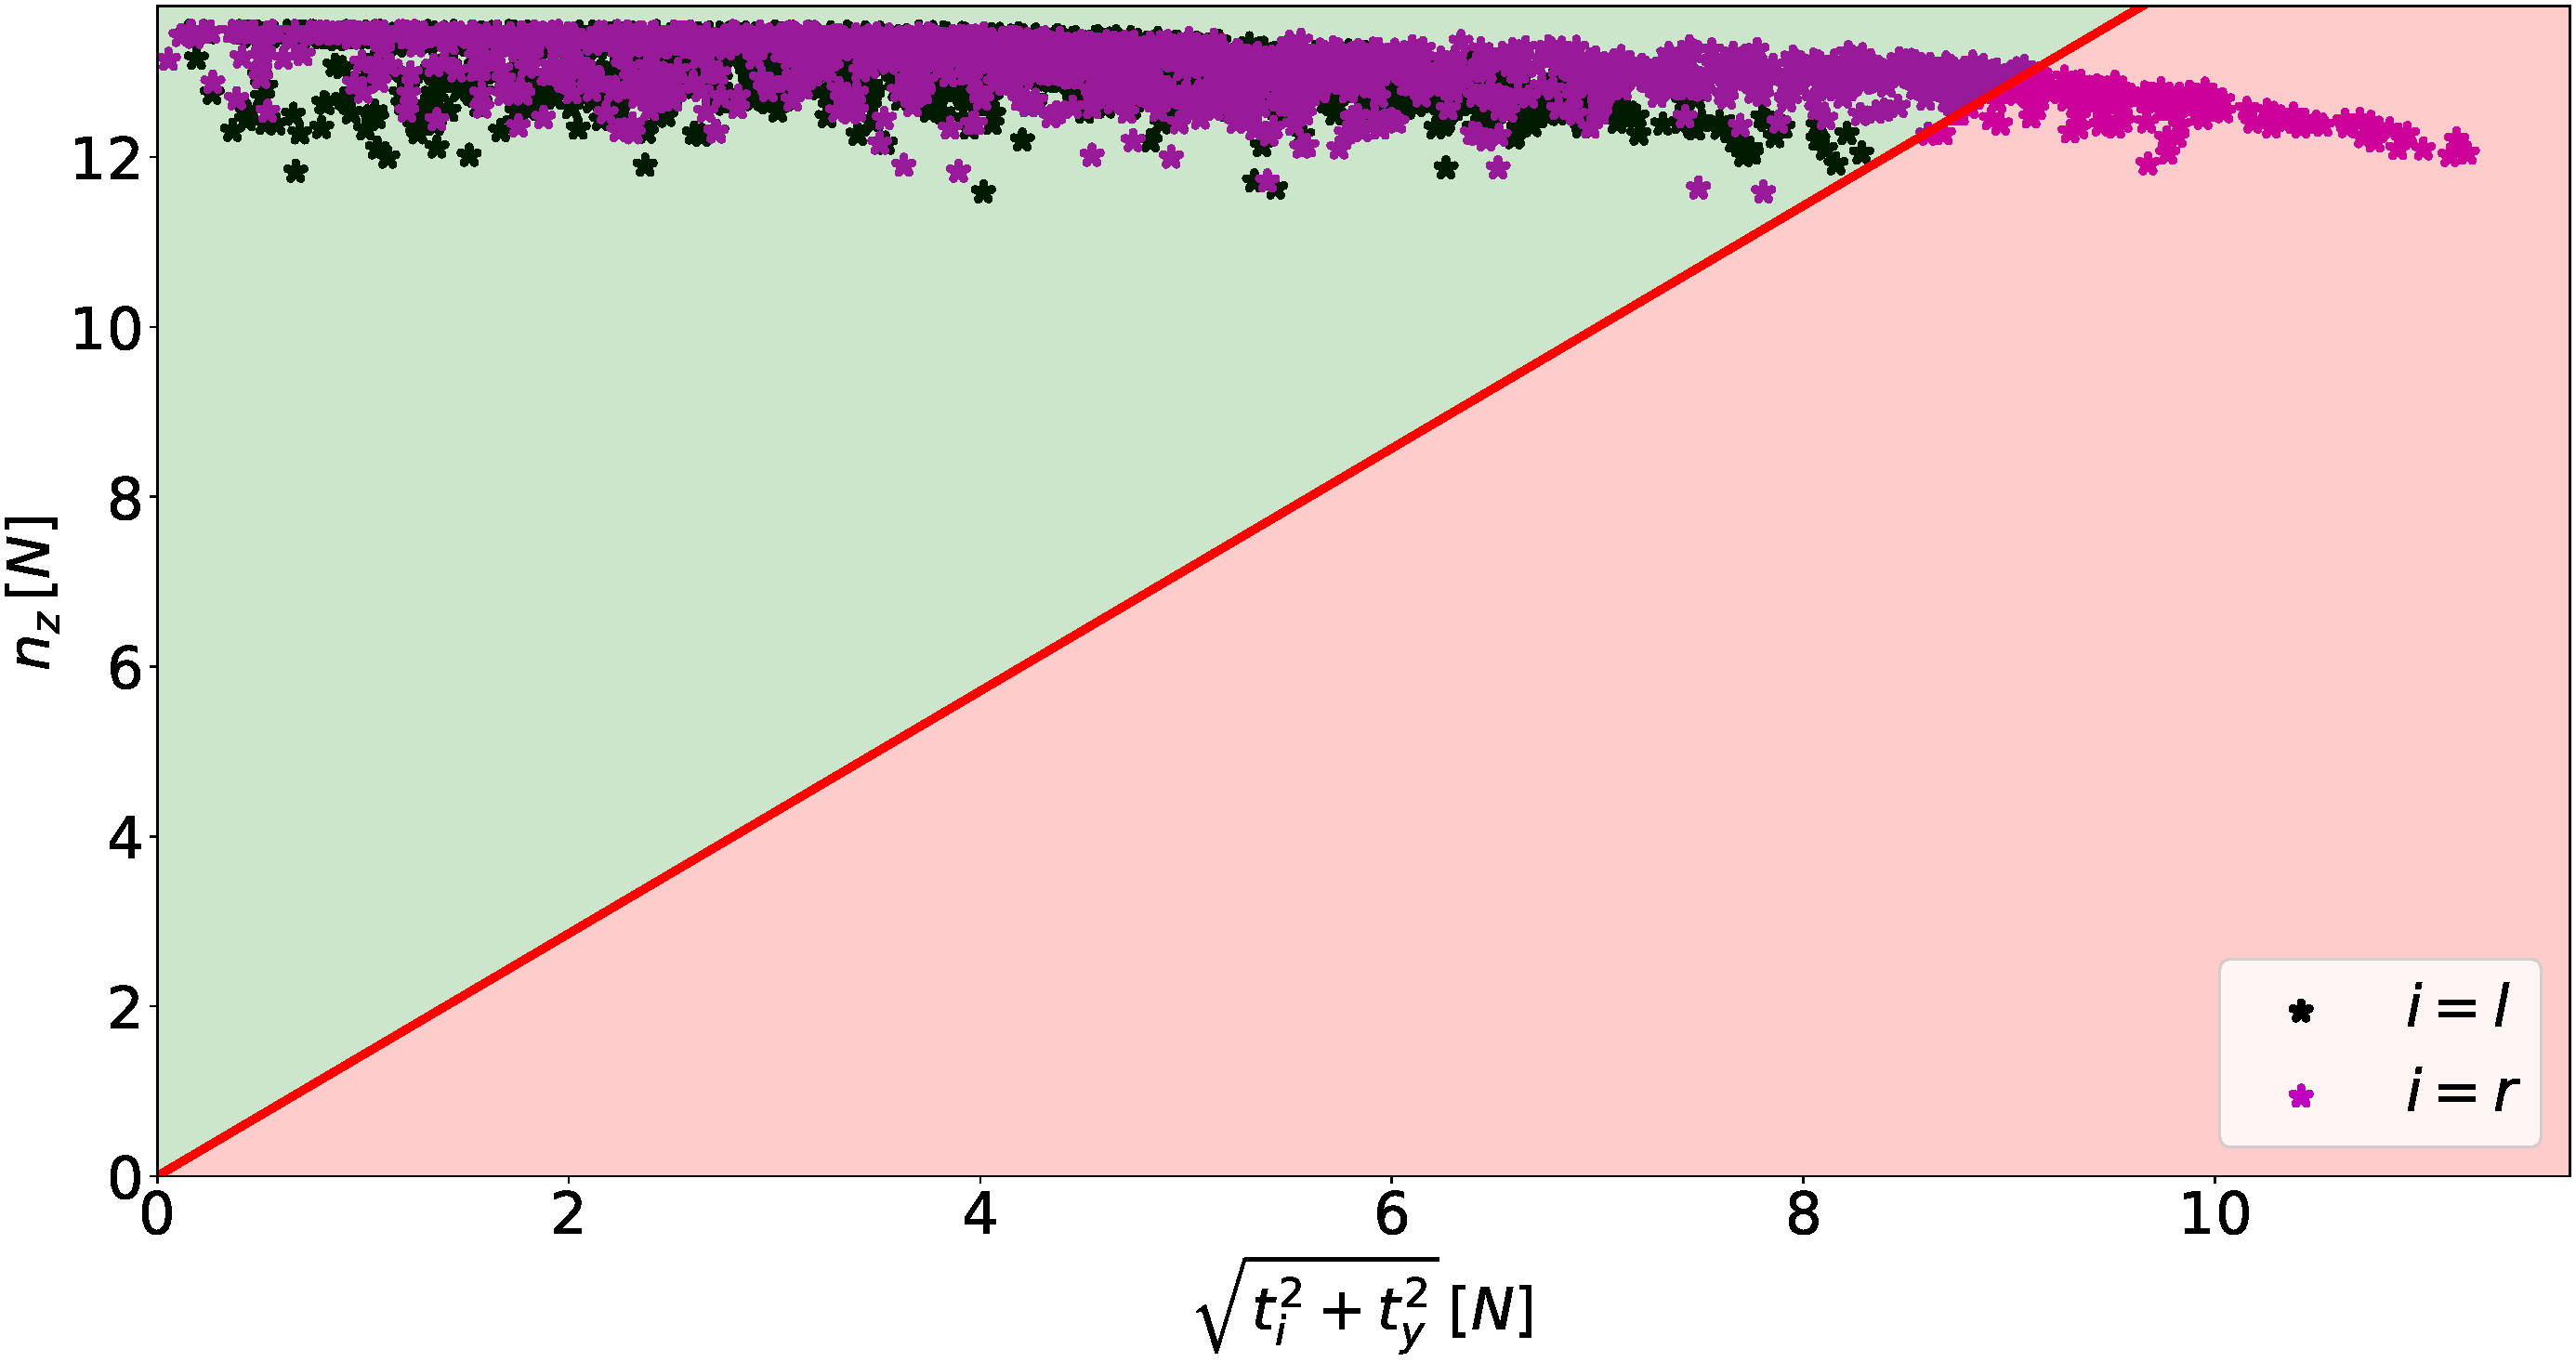
\includegraphics[width=0.49\linewidth]{Figures/Real time one stage OCP on rough terrain/Rough and uneven terrain map/forces_cone_4.pdf}}
    \subfigure[Very low rate of change.]{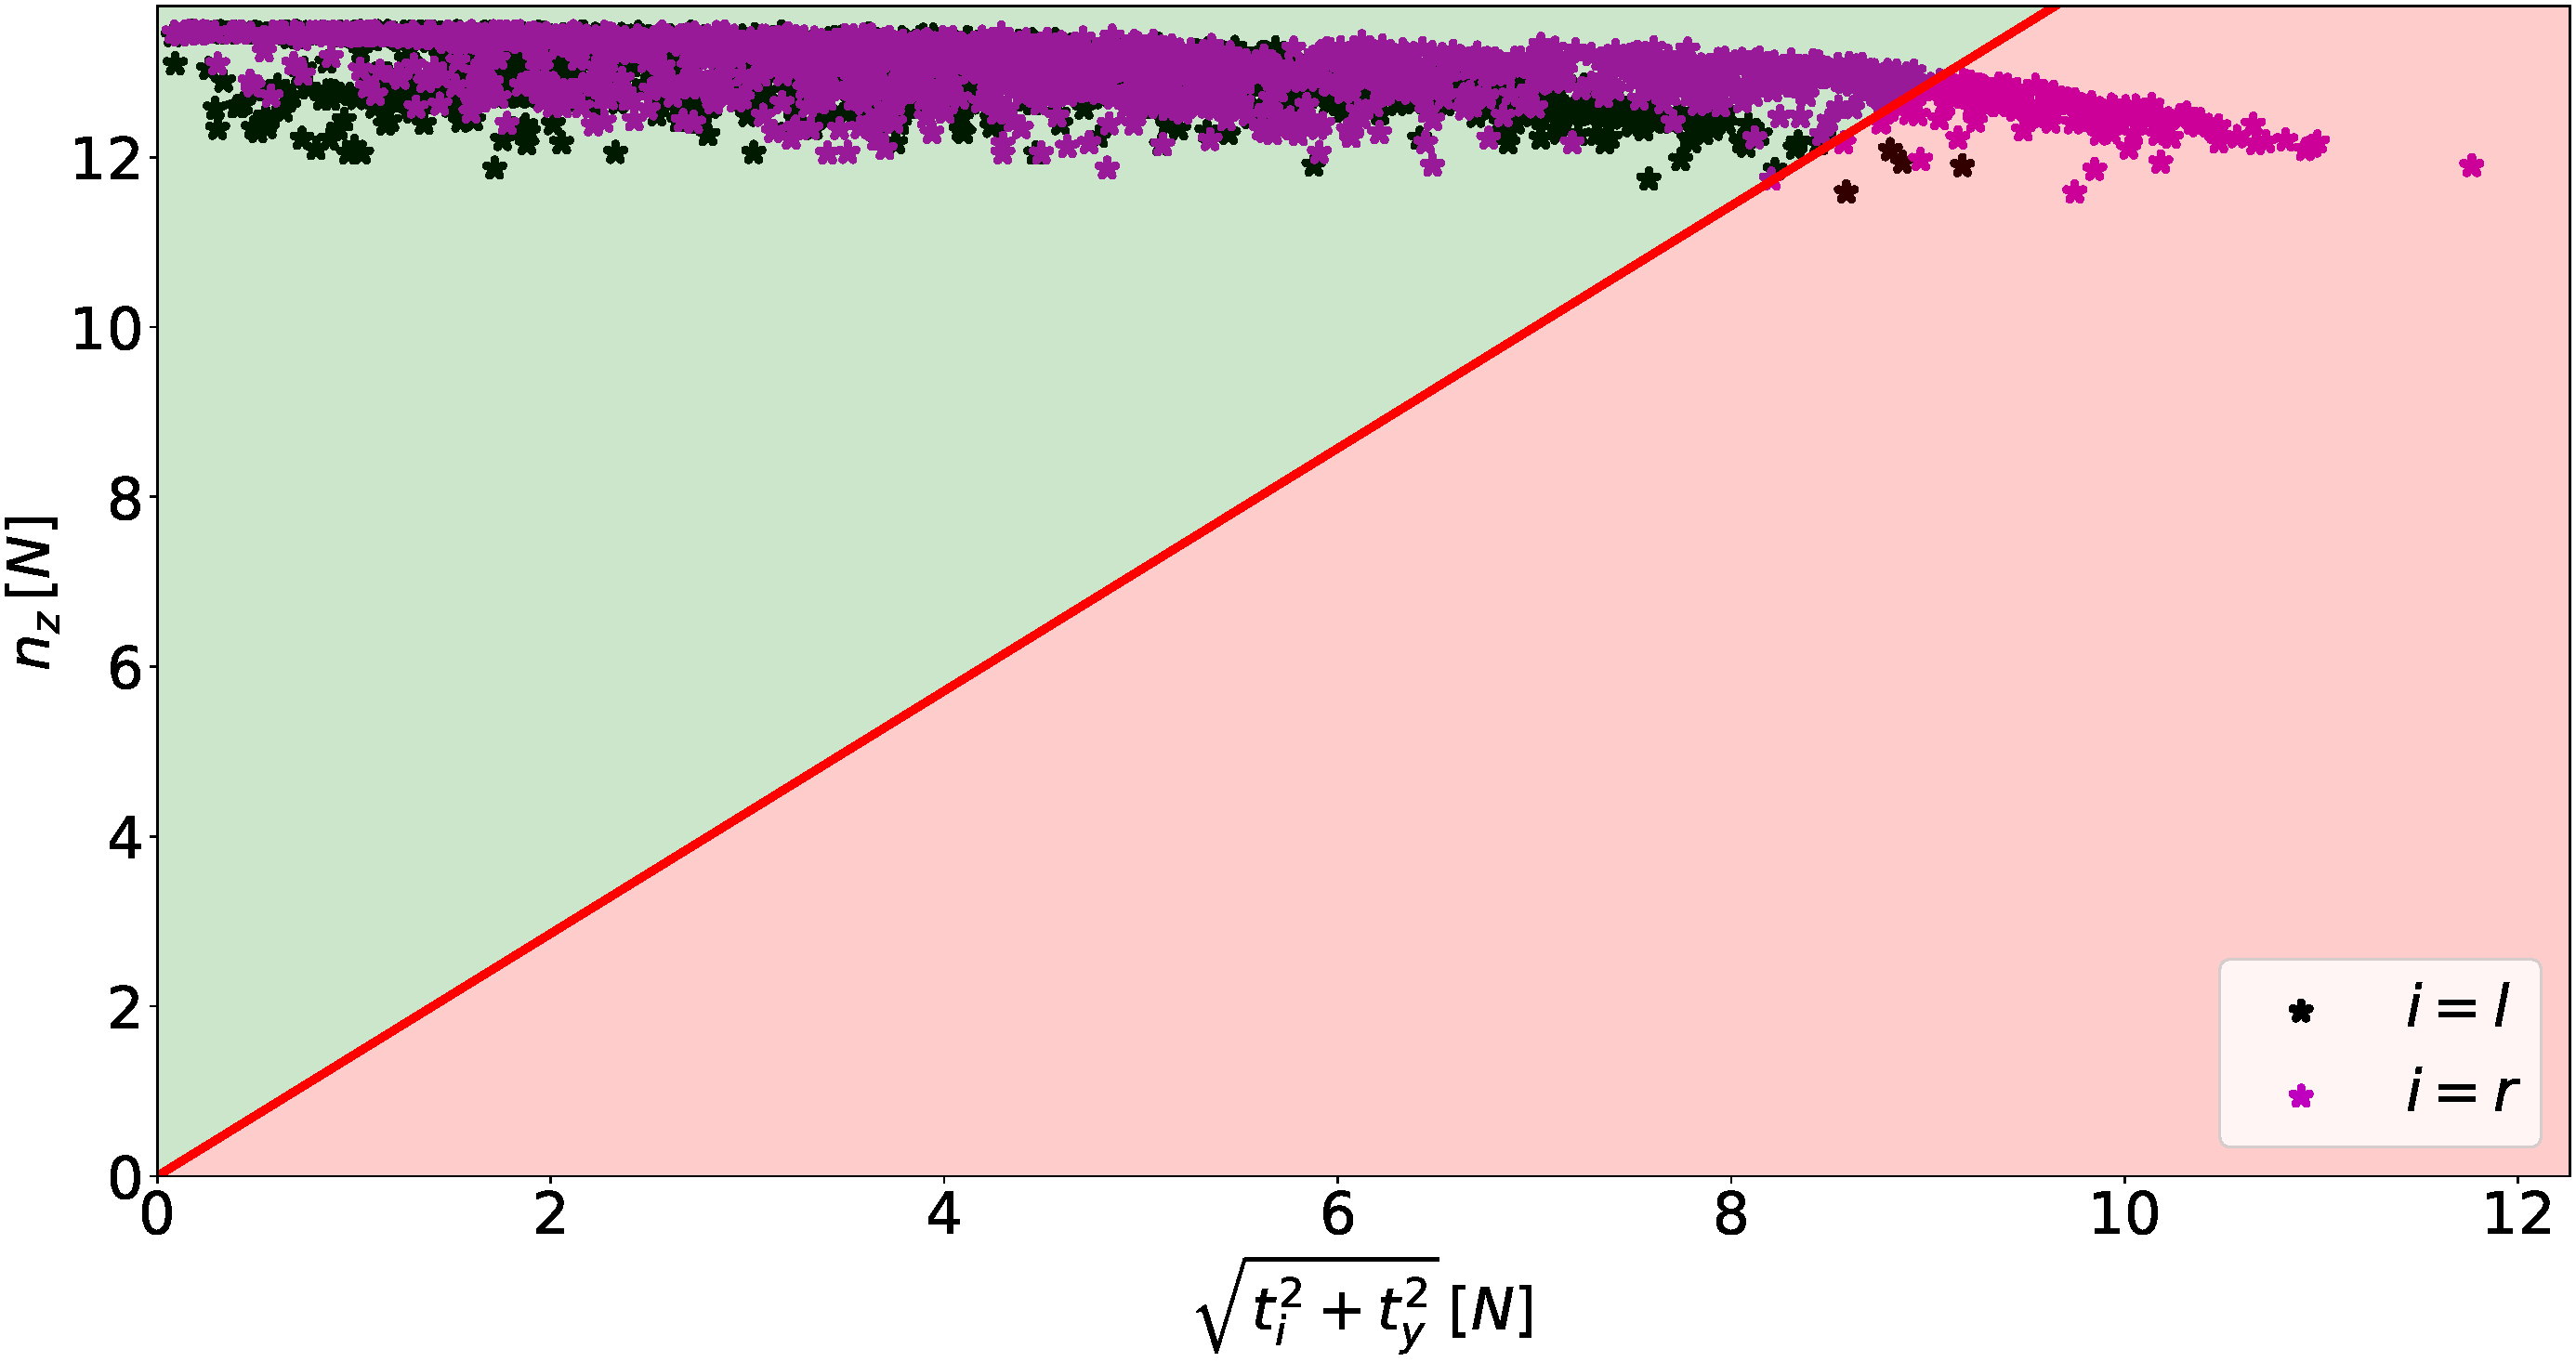
\includegraphics[width=0.49\linewidth]{Figures/Real time one stage OCP on rough terrain/Rough and uneven terrain map/forces_cone_5.pdf}}
  \end{subfigmatrix}
  \caption{Location of wheel traction force within the Coulomb friction cone with respect to each solver.}
  \label{fig:RoughUnevenTerrainForcesConeHill}
\end{figure}

\begin{figure}[!htb]
  \begin{subfigmatrix}{3}
    \subfigure[Traction forces with solver \ti{Moderate rate of change}.]{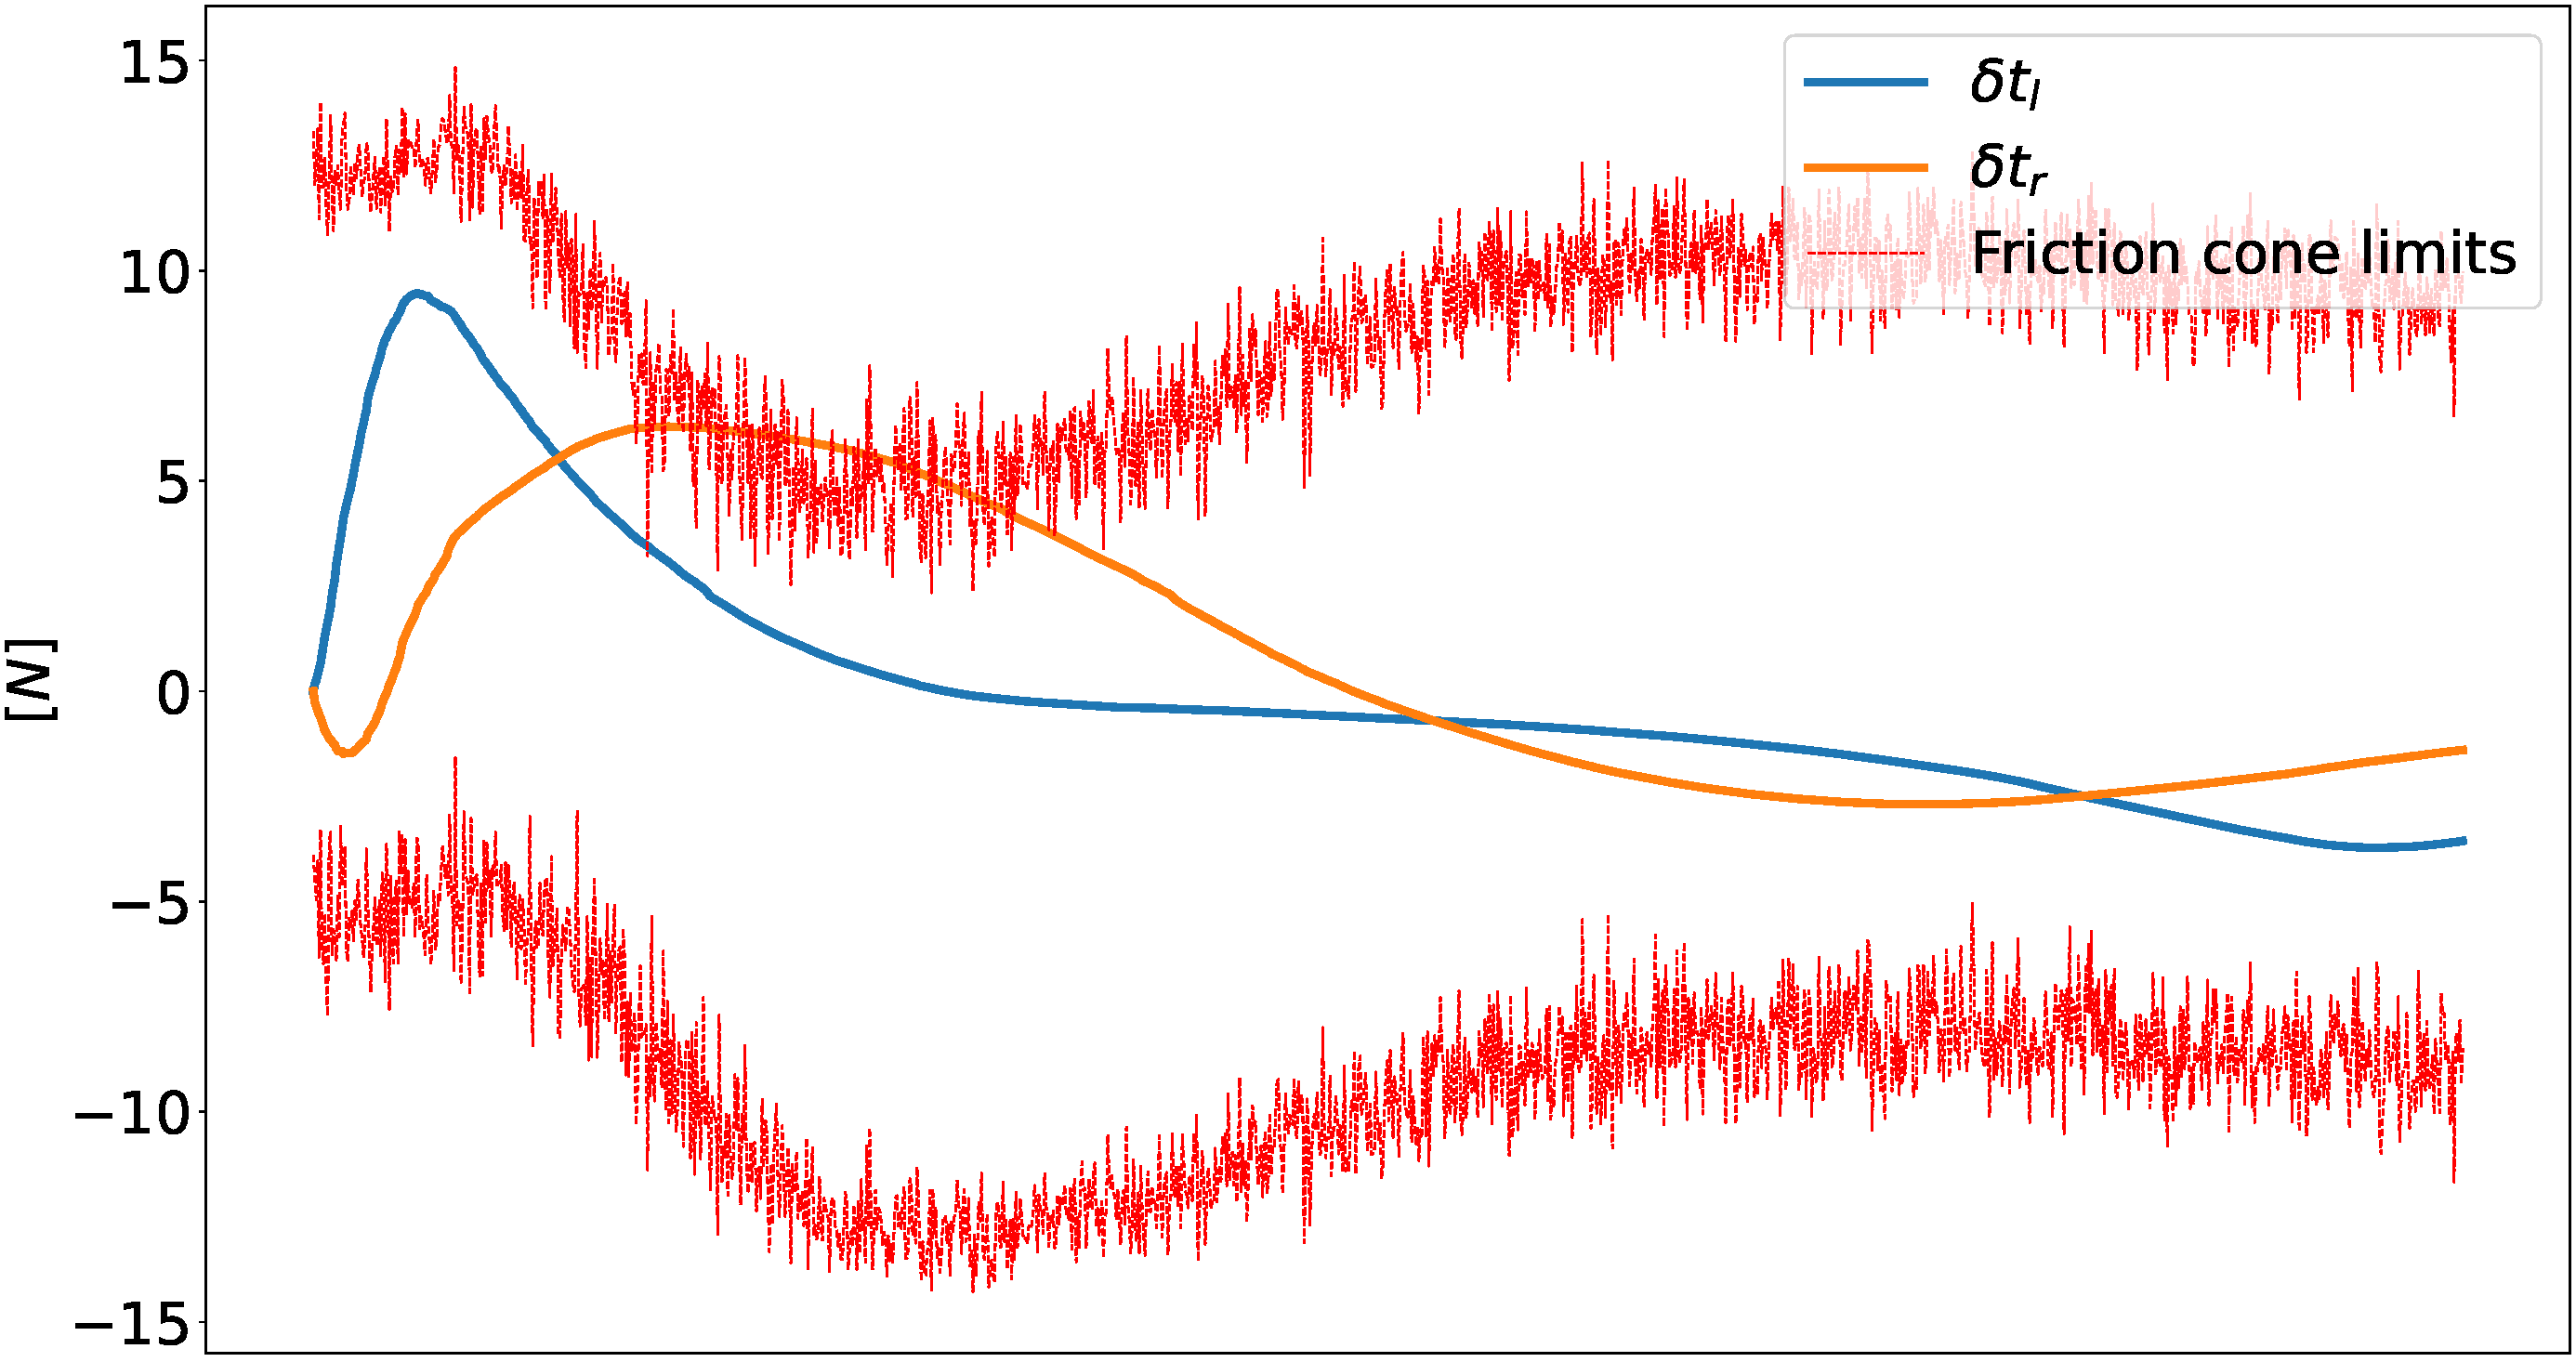
\includegraphics[width=0.325\linewidth]{Figures/Real time one stage OCP on rough terrain/Rough and uneven terrain map/forces_curve_solver_2.pdf}}
    \subfigure[Traction forces with solver \ti{Energy saver}.]{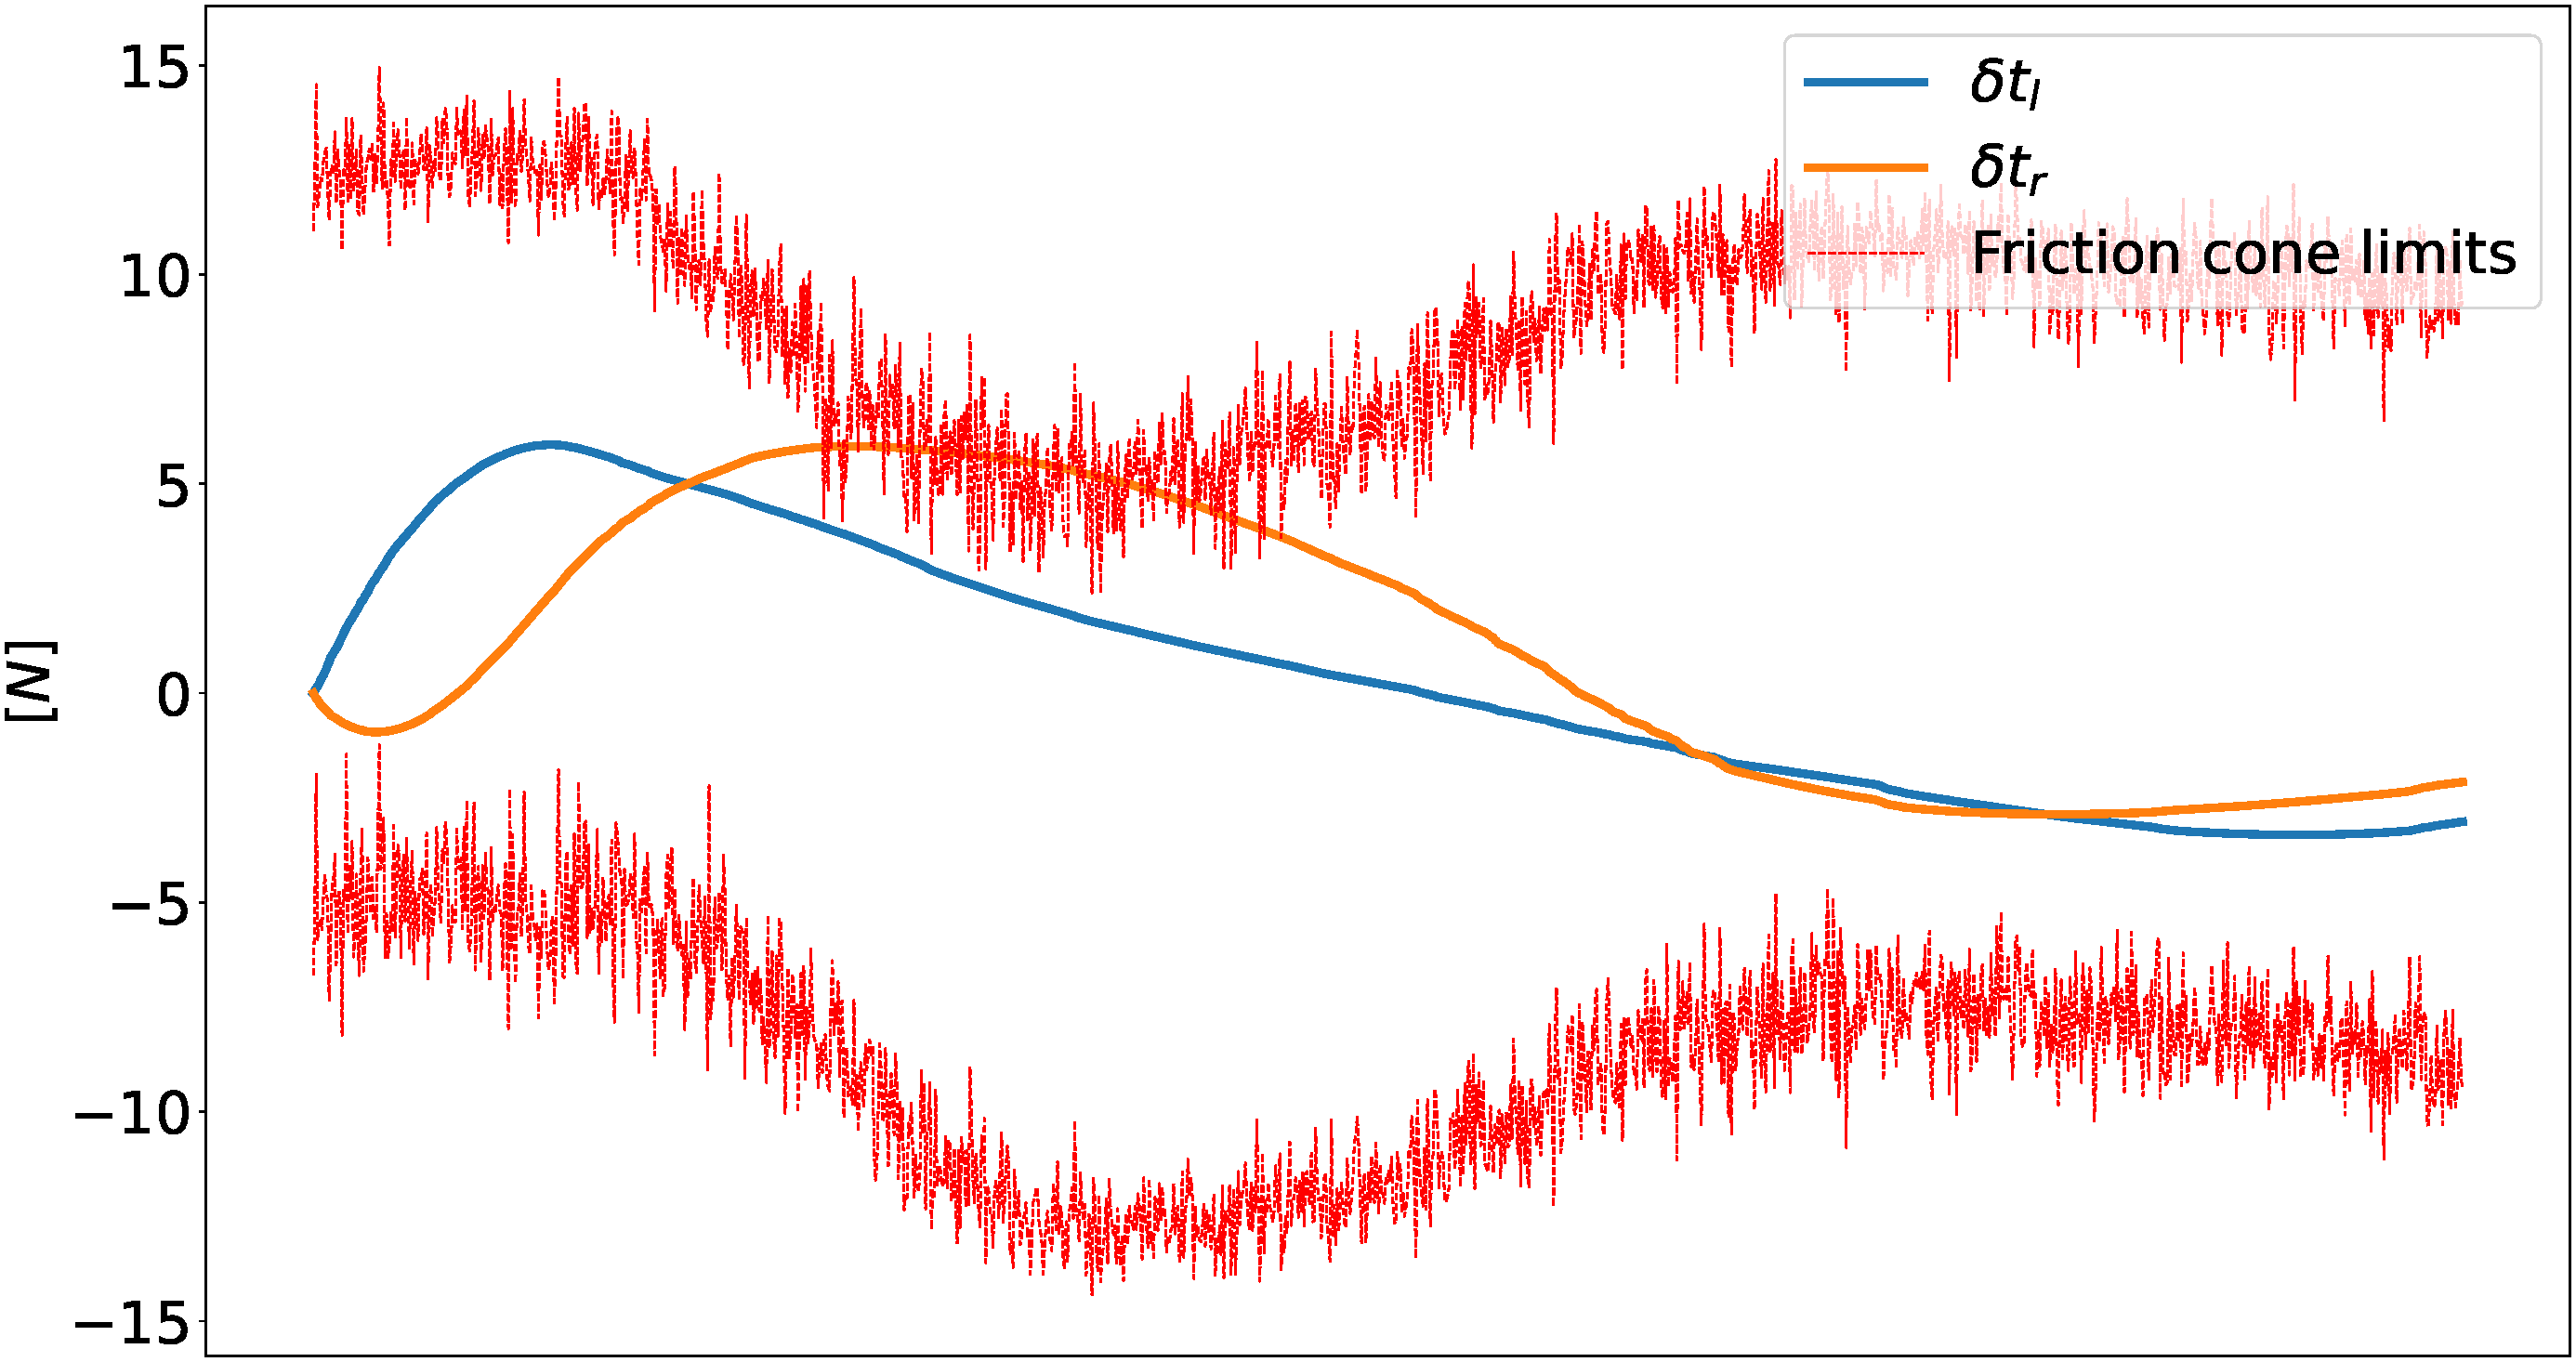
\includegraphics[width=0.325\linewidth]{Figures/Real time one stage OCP on rough terrain/Rough and uneven terrain map/forces_curve_solver_4.pdf}}
    \subfigure[Traction rates with solvers \ti{Moderate rate of change} and \ti{Energy saver}.]{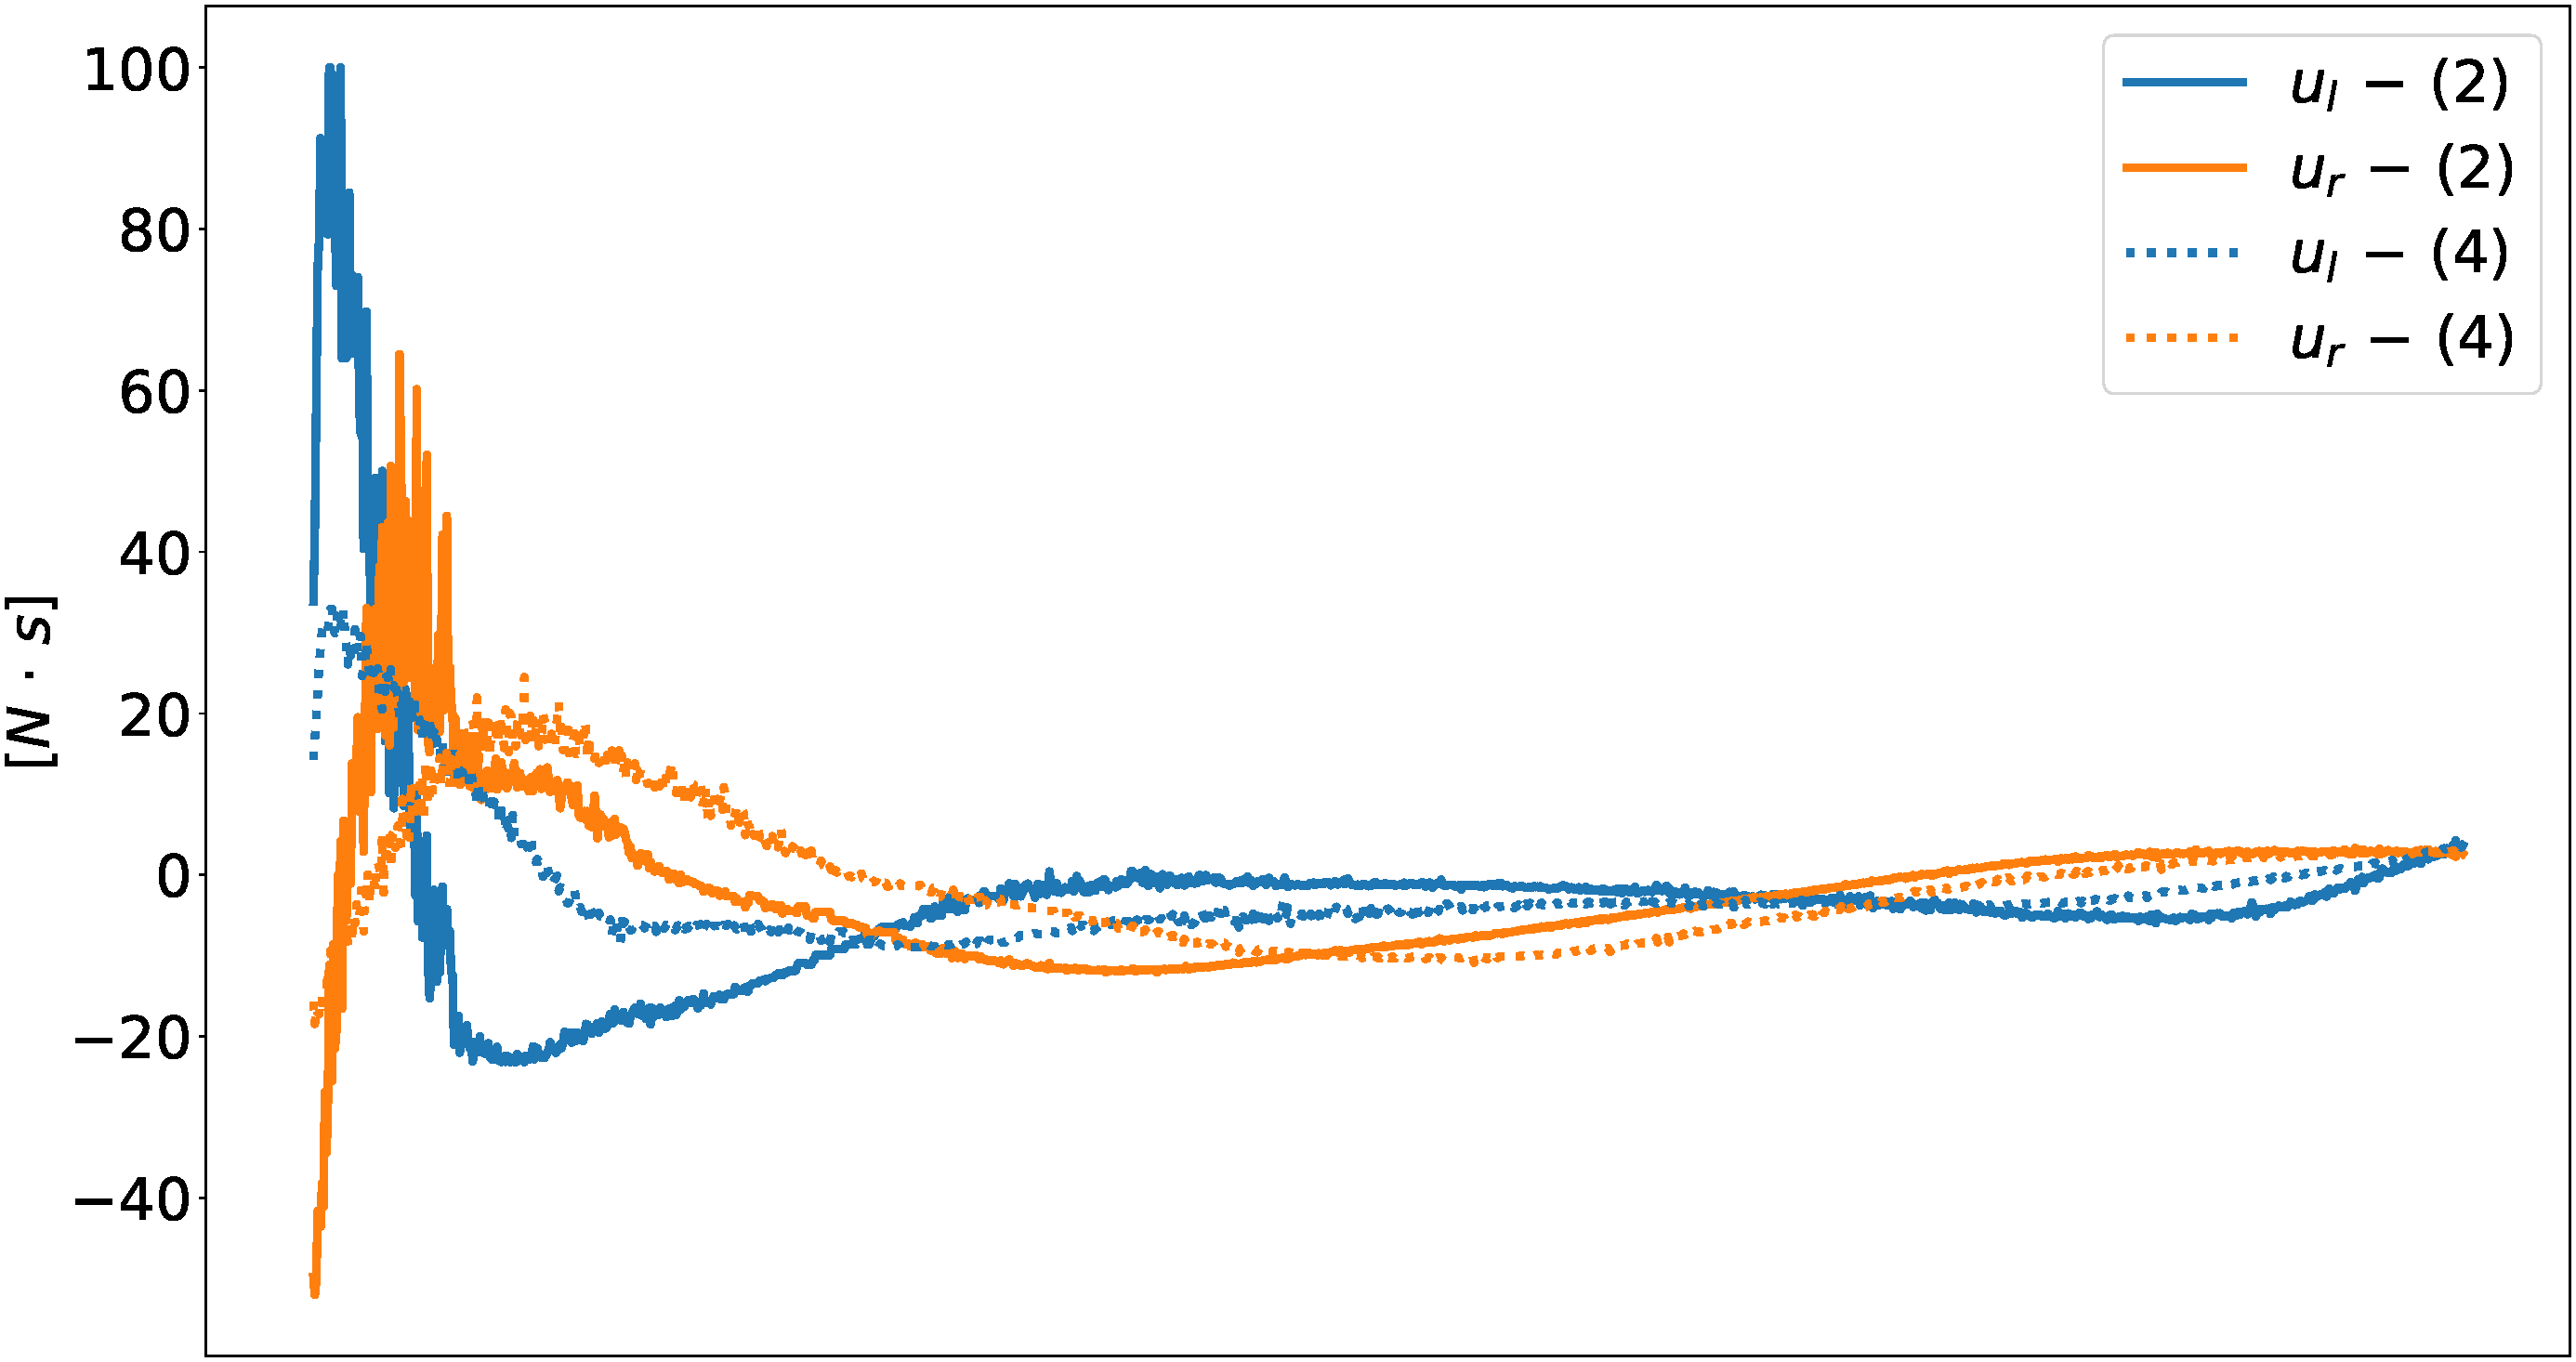
\includegraphics[width=0.325\linewidth]{Figures/Real time one stage OCP on rough terrain/Rough and uneven terrain map/rate_forces_curve_solvers_2_4.pdf}
    \label{subfig:traction_rates_solvers_2_4}}
  \end{subfigmatrix}
  \caption{Traction forces and traction rates.}
  \label{fig:Forces_ForcesRates_Curves}
\end{figure}

Once more, the performance of the tested solvers is presented in table \ref{tab:RoughTerrainSolverPerformanceShortTrack}. All solvers are computationally feasible as the timeouts are very rare and the loop times are far away from the sampling time $T_s$. On other hand, the optimal cost increases when more weights are placed in the traction forces and on its rates. However, avoiding slippage to prevent hazardous events comes first, so placing higher weights on traction rates is a better strategy. These high weights on traction rates also decrease the cumulative traction energy spent by the vehicle, which is desired as a way to save the battery. 

Apart from solver \ti{Fast rate of change} where slippage happens a lot, slippage became much less frequent in the remaining controllers. Moreover, most of the solver fails arise when slippage takes place. As a thumbs up rule, these results have shown that placing higher weights on the traction rates help with avoiding slippage and on saving the battery.

\begin{equation}
\begin{matrix}
\delta\Traction_{min} = \frac{-k-\sqrt{k^2 - 4\,p}}{2} & \delta\Traction_{max} = \frac{-k+\sqrt{k^2 - 4\,p}}{2}\\
k = \frac{m\,g\,\sin(\pitch)}{2}  & p = \frac{(m\,g)^2}{16} \, \left[ \left(\cos(\pitch)\,\sin(\roll)\right)^2 + \sin^2(\pitch)- \left(\FrictionCoefficient\,\cos(\roll)\,\cos(\pitch)\right)^2 \right]
\end{matrix}
\label{eq:forcesLimits}
\end{equation}

\begin{table}[!htb]
  \caption[Solver performance on hilly terrain.]{Solvers performance on rough, uneven terrain. On every solver, one timeout was recorded.}
  \label{tab:RoughTerrainSolverPerformanceShortTrack}
  \renewcommand{\arraystretch}{1.2}
  \centering
  \small
  \begin{tabular}[]{lcccccc}
	\toprule
	& \shortstack{Loop\\time [ms]} & \shortstack{Solver\\time [ms]} & Cost & \shortstack{Solver fails\\/slippage[\%]} & \shortstack{Cumulative\\energy}[$N \cdot s$]\\
	\midrule
	\shortstack{Fast rate\\of change} & $(6.09) \pm (4.09)$ & $(1.65) \pm (0.64)$ & $(1236.11) \pm (1144.58)$ & $99.35$ & $9.22$\\
	\shortstack{Moderate rate\\of change} & $(5.95) \pm (4.46)$ & $(1.60) \pm (0.51)$ & $(17.29) \pm (49.18)$ & $87.67$ & $3.11$\\
	\shortstack{Low rate\\of change} & $(5.76) \pm (3.32)$ & $(1.56) \pm (0.40)$ & $(94.00) \pm (184.79)$ & $80.16$ & $2.90$\\
	\shortstack{Energy\\saver} & $(6.19) \pm (3.80)$ & $(1.68) \pm (0.65)$ & $(87.52) \pm (177.70)$ & $88.24$ & $1.84$\\
	\shortstack{Very low\\rate of change} & $(5.63) \pm (3.18)$ & $(1.55) \pm (0.44)$ & $(147.76) \pm (242.53)$ & $84.56$ & $3.62$\\
  	\bottomrule
  \end{tabular}
\end{table}

\subsubsection*{Initial pose away from reference (with solver \ti{Low rate of change})}

Figure \ref{fig:startAwayPathTrackingRough} presents the path tracking results of solver \ti{Low rate of change} with different initial poses that are away from the reference. Table \ref{tab:RoughTerrainSolverPerformance} denotes the respective performance metrics.

This configuration has proved to be one that works well when it comes to guide the mobile robot back to the reference. When the initial yaw is very different from the reference heading, the solver is asked to perform agressive turns to address this deviation. This is why the performance of the solver degrades significantly for the \textcolor{tabblue}{blue}, \textcolor{tabpink}{pink}, \textcolor{tabbrown}{brown} and \textcolor{tabolive}{olive} simulations. 

Fortunately, slippage is rare and the the solver mostly fails when slippage happens. The loop time, $T_c$, is smaller than $T_s$ so the controller is computationally feasible for real-time control.

\begin{figure}[!htb]
  \centering
  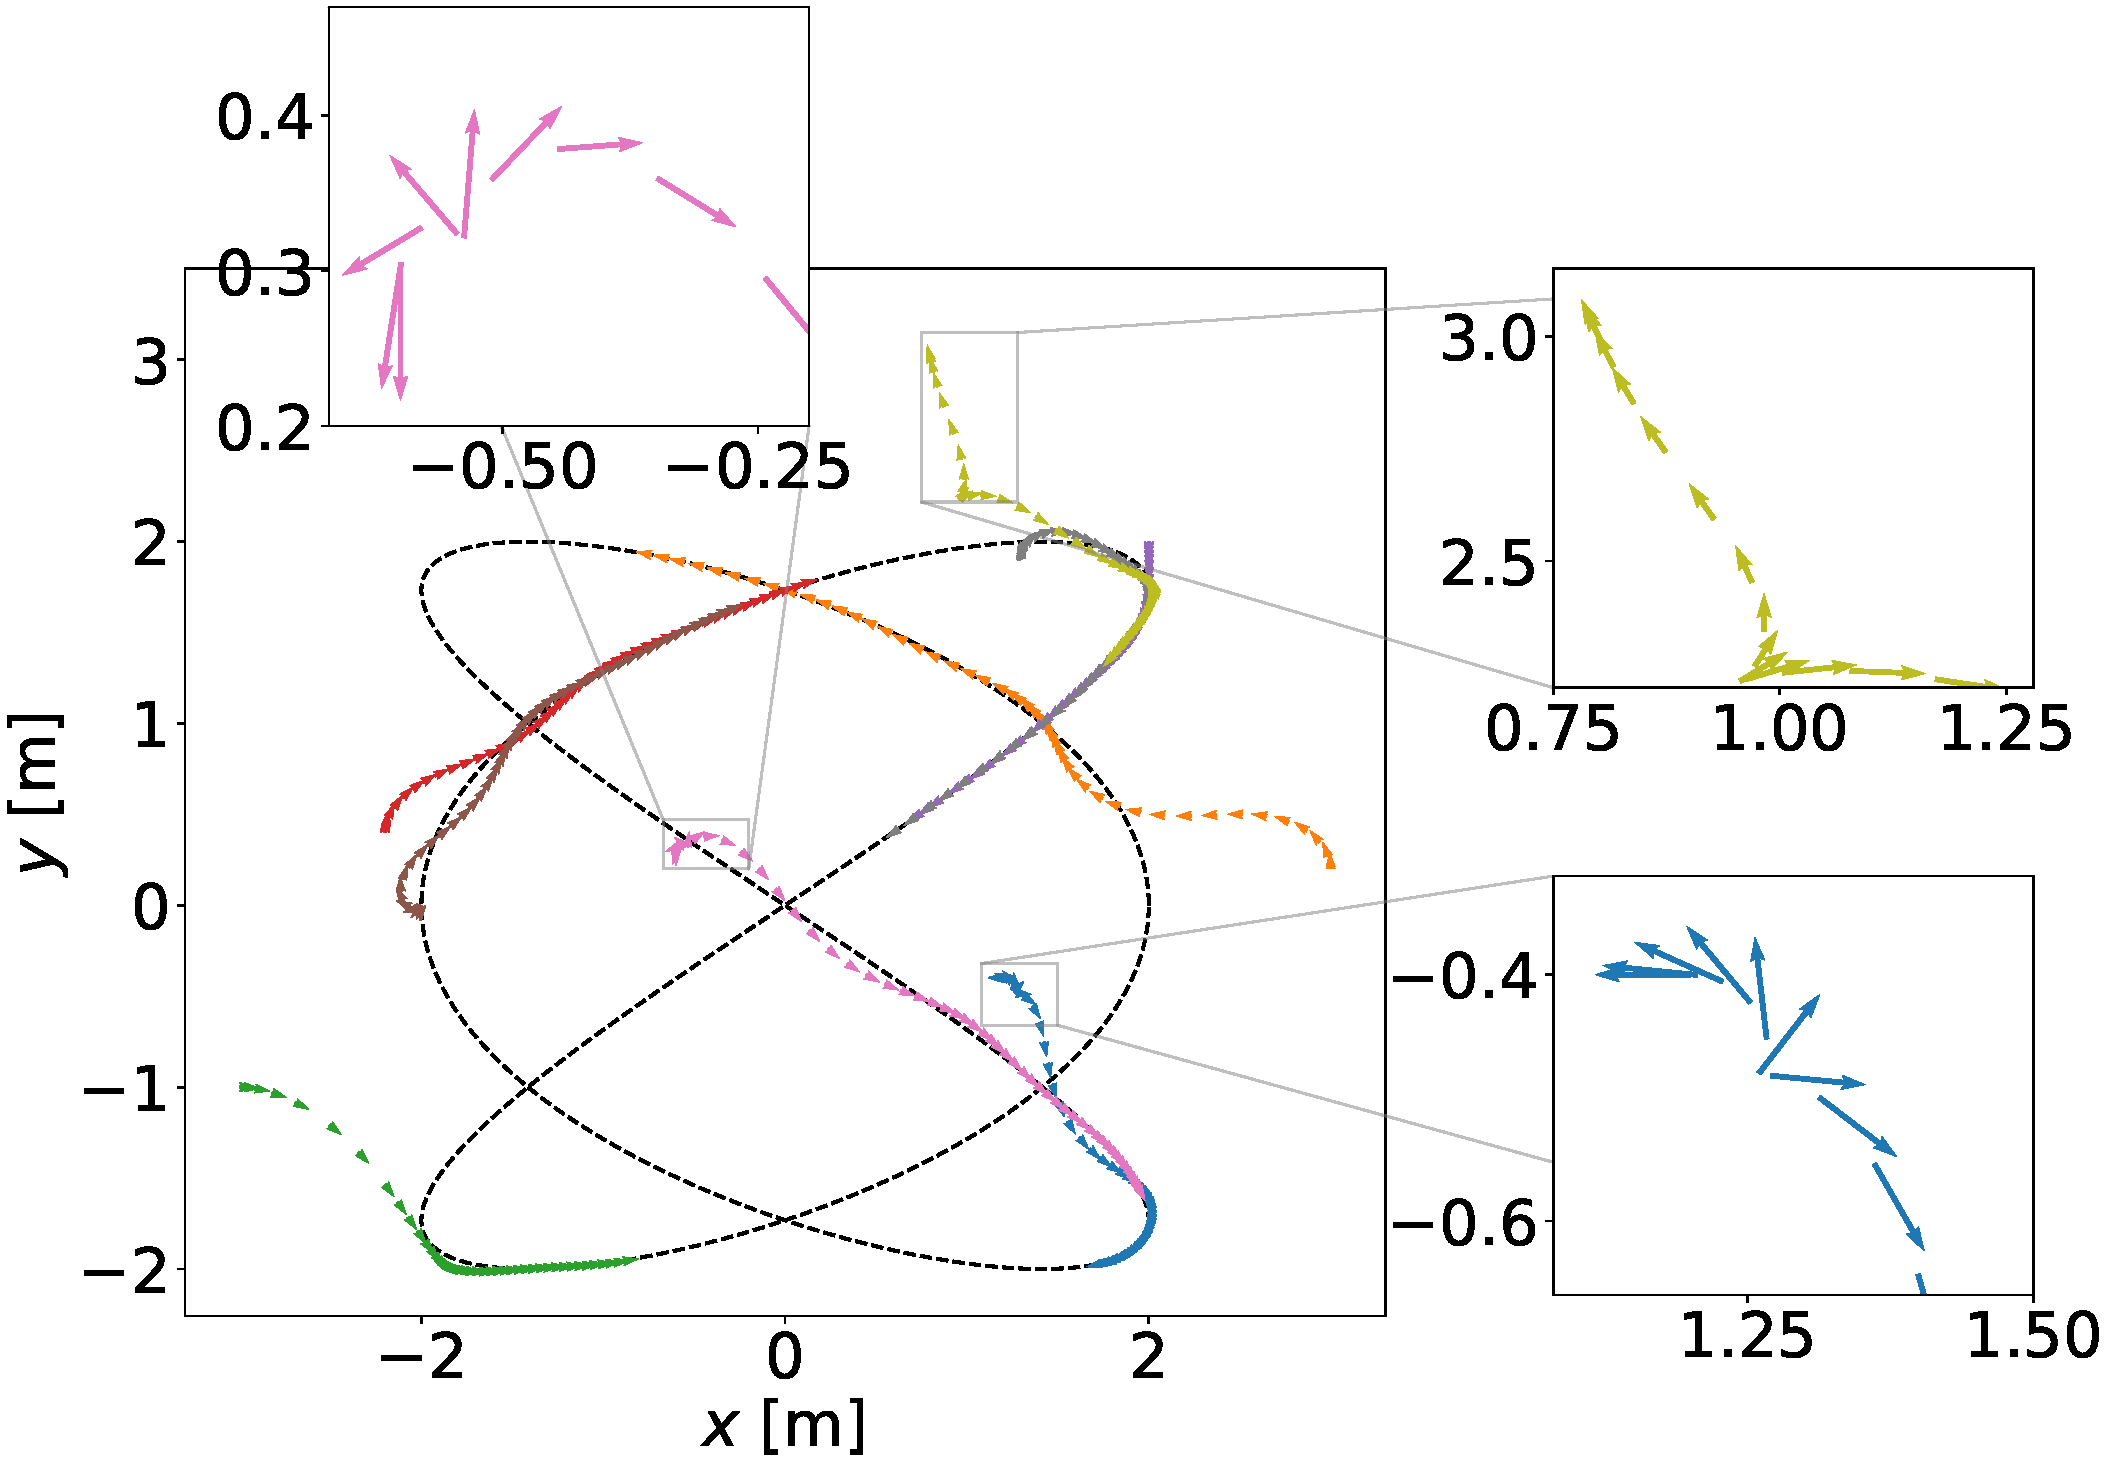
\includegraphics[width=0.99\textwidth]{Figures/Real time one stage OCP on rough terrain/Rough and uneven terrain map/Start_away_from_ref.pdf}
  \caption[Path tracking with initial position away from reference on rough terrain.]{Path tracking with initial position away from reference on rough terrain, where $a=1.0,\,b=1.0,\,c=0.4$.}
  \label{fig:startAwayPathTrackingRough}
\end{figure}

\begin{table}[!htb]
  \caption[Solver \ti{low rate of change} performance on rough, uneven terrain. One timeout was recorded.]{Solver \ti{low rate of change} performance on rough, uneven terrain. One timeout was recorded.}
  \label{tab:RoughTerrainSolverPerformance}
  \renewcommand{\arraystretch}{1.2}
  \centering
  \begin{tabular}[]{lccccc}
	\toprule
	& \shortstack{Loop\\time [ms]} & \shortstack{Solver\\time [ms]} & Cost & \shortstack{Slippage\\events [\%]} & Solver fails [\%]\\
	\midrule
	\textcolor{tabblue}{Blue} & $(5.41) \pm (3.14)$ & $(1.38) \pm (0.39)$ & $(20.78) \pm (64.48)$ & $0.04$ & $0.0$\\
	\textcolor{taborange}{Orange} & $(6.57) \pm (2.16)$ & $(1.78) \pm (0.67)$ & $(13.54) \pm (45.85)$ & $0.02$ & $0.0$\\
	\textcolor{tabgreen}{Green} & $(5.22) \pm (1.71)$ & $(1.33) \pm (0.41)$ & $(7.97) \pm (26.32)$ & $0.0$ & $0.0$\\
	\textcolor{tabred}{Red} & $(4.98) \pm (1.42)$ & $(1.28) \pm 0.29$ & $(2.87) \pm (7.73)$ &  $0.0$ & $0.0$\\
	\textcolor{tabpurple}{Purple} & $(5.08) \pm (1.28)$ & $(1.32) \pm (0.34)$ & $(0.20) \pm (0.67)$ & $0.0$ & $0.0$\\
	\textcolor{tabbrown}{Brown} & $(4.85) \pm (2.12)$ & $(1.30) \pm (0.32)$ & $(9.62) \pm (31.68)$ & $0.42$ & $0.24$\\
	\textcolor{tabpink}{Pink} & $(5.58) \pm (2.53)$ & $(1.49) \pm (0.43)$ & $(29.02) \pm (135.03)$ & $0.38$ & $0.18$\\
	\textcolor{tabgray}{Gray} & $(7.20) \pm (2.22)$ & $(1.92) \pm (0.71)$ & $(2.76) \pm (8.56)$ & $0.0$ & $0.0$\\
	\textcolor{tabolive}{Olive} & $(5.22) \pm (2.94)$ & $(1.34) \pm (0.36)$ & $(39.19) \pm (97.97)$ & $0.88$ & $0.66$\\
  	\bottomrule
  \end{tabular}
\end{table}

The only timeout happens in the first iteration where the initial guess of the solver is searched, so additional overhead is present there. Then, figure \ref{fig:RoughUnevenTerrainForcesConeStartAway} presents the traction forces within the Coulomb friction cone for each simulation. Slippage takes place at high inclination locations, as the normal force $n_z$ is typically lower in these events. Finally, figure \ref{fig:referenceTourStats} depicts the simulation results of a full tour to the reference curve. The same trends come up, although it is useful to point out to the fact that the solver fails when slippage happens.  Moreover, traction rates have a bumpy behaviour due to the need of the controller to balance the vehicle on irregular terrain.

\begin{figure}[!htb]
  \begin{subfigmatrix}{9}
    \subfigure[\textcolor{tabblue}{Blue}]{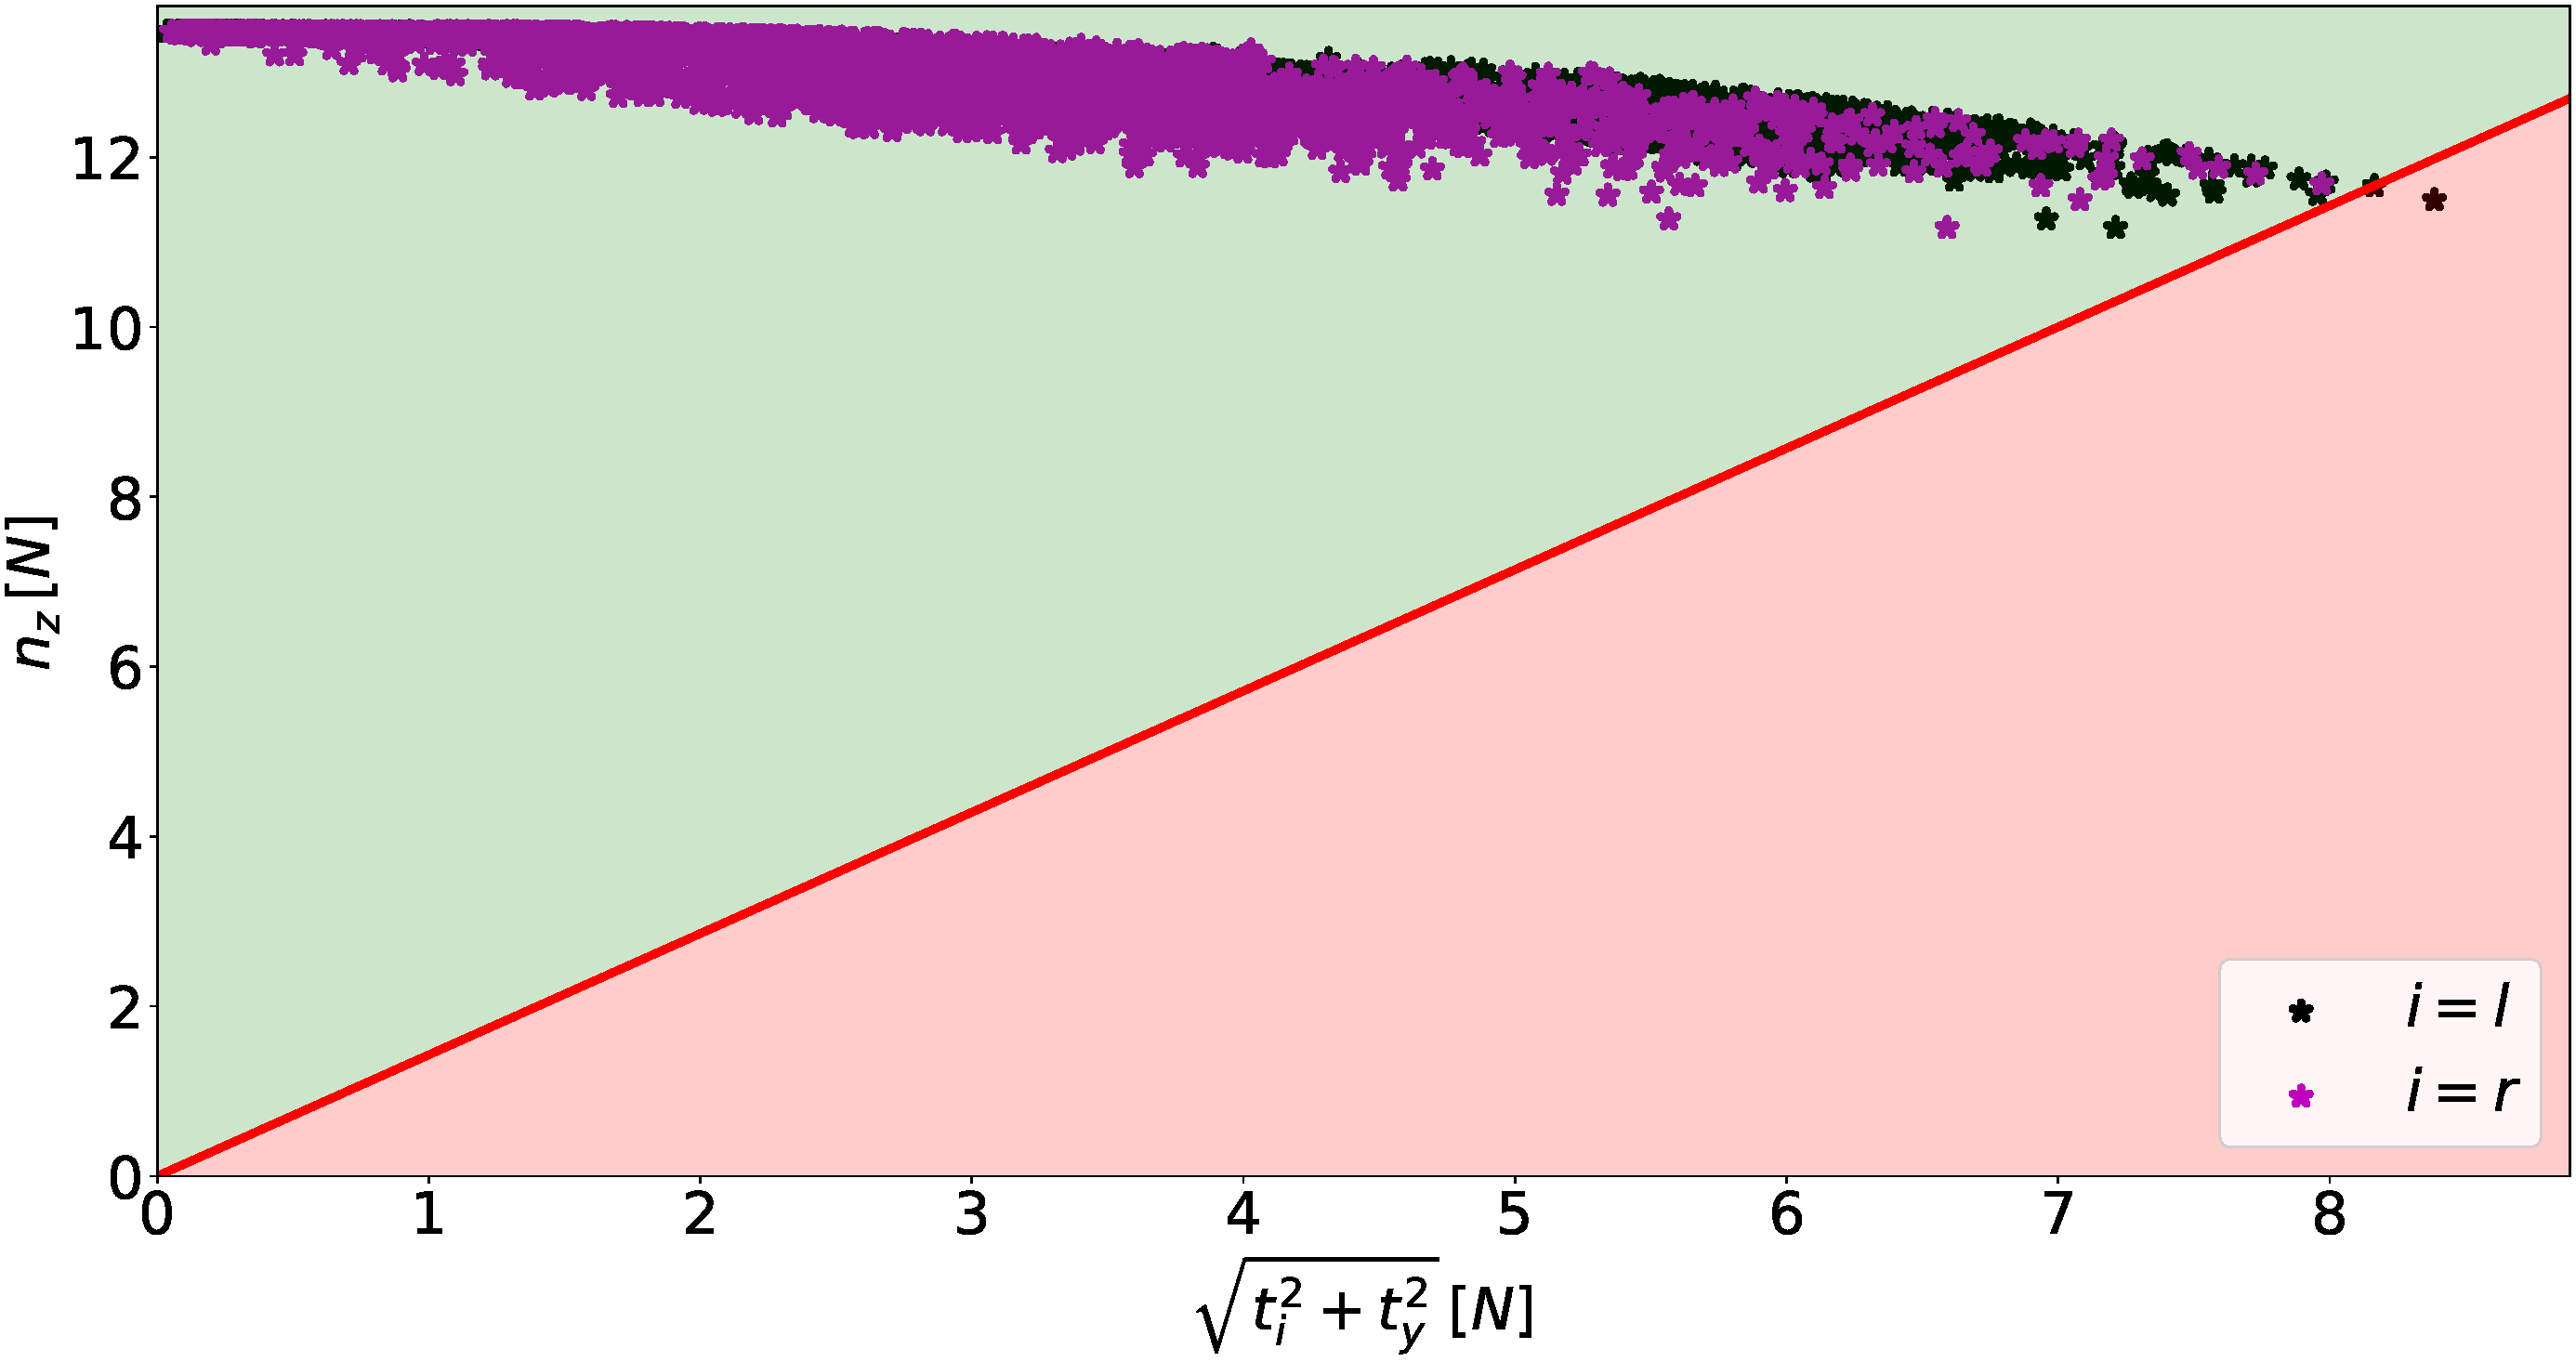
\includegraphics[width=0.325\linewidth]{Figures/Real time one stage OCP on rough terrain/Rough and uneven terrain map/forces_cone_tabblue.pdf}}
    \subfigure[\textcolor{taborange}{Orange}]{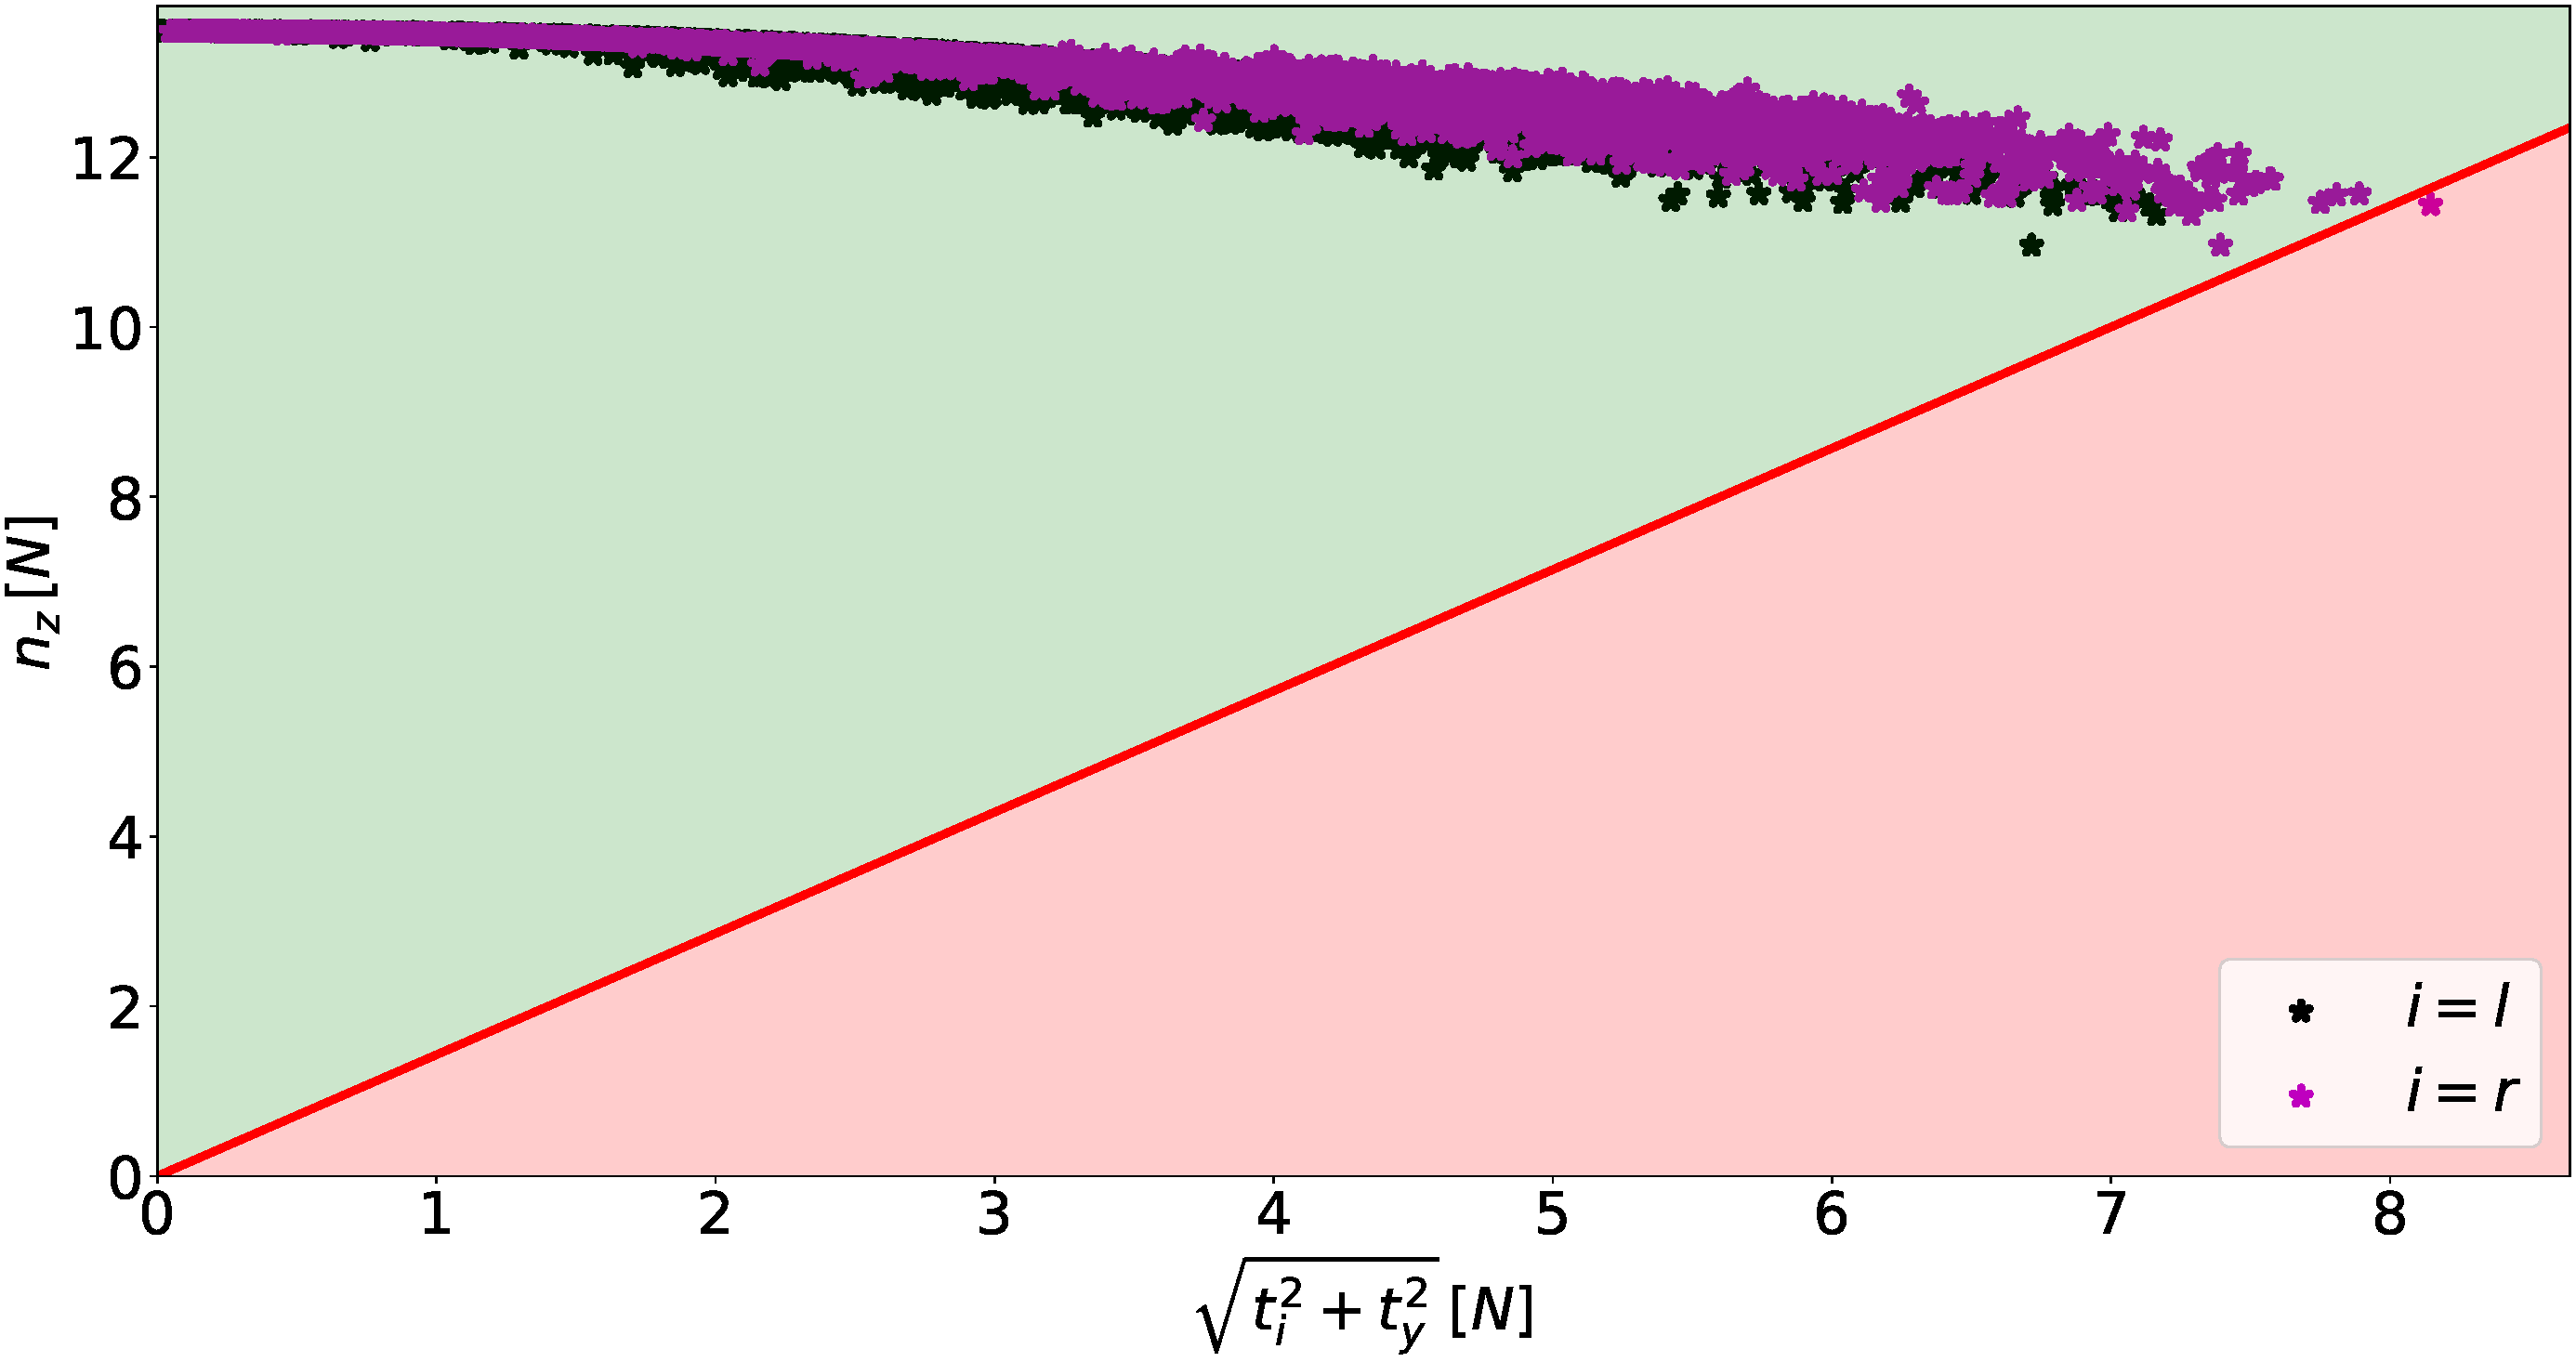
\includegraphics[width=0.325\linewidth]{Figures/Real time one stage OCP on rough terrain/Rough and uneven terrain map/forces_cone_taborange.pdf}}
    \subfigure[\textcolor{tabgreen}{Green}]{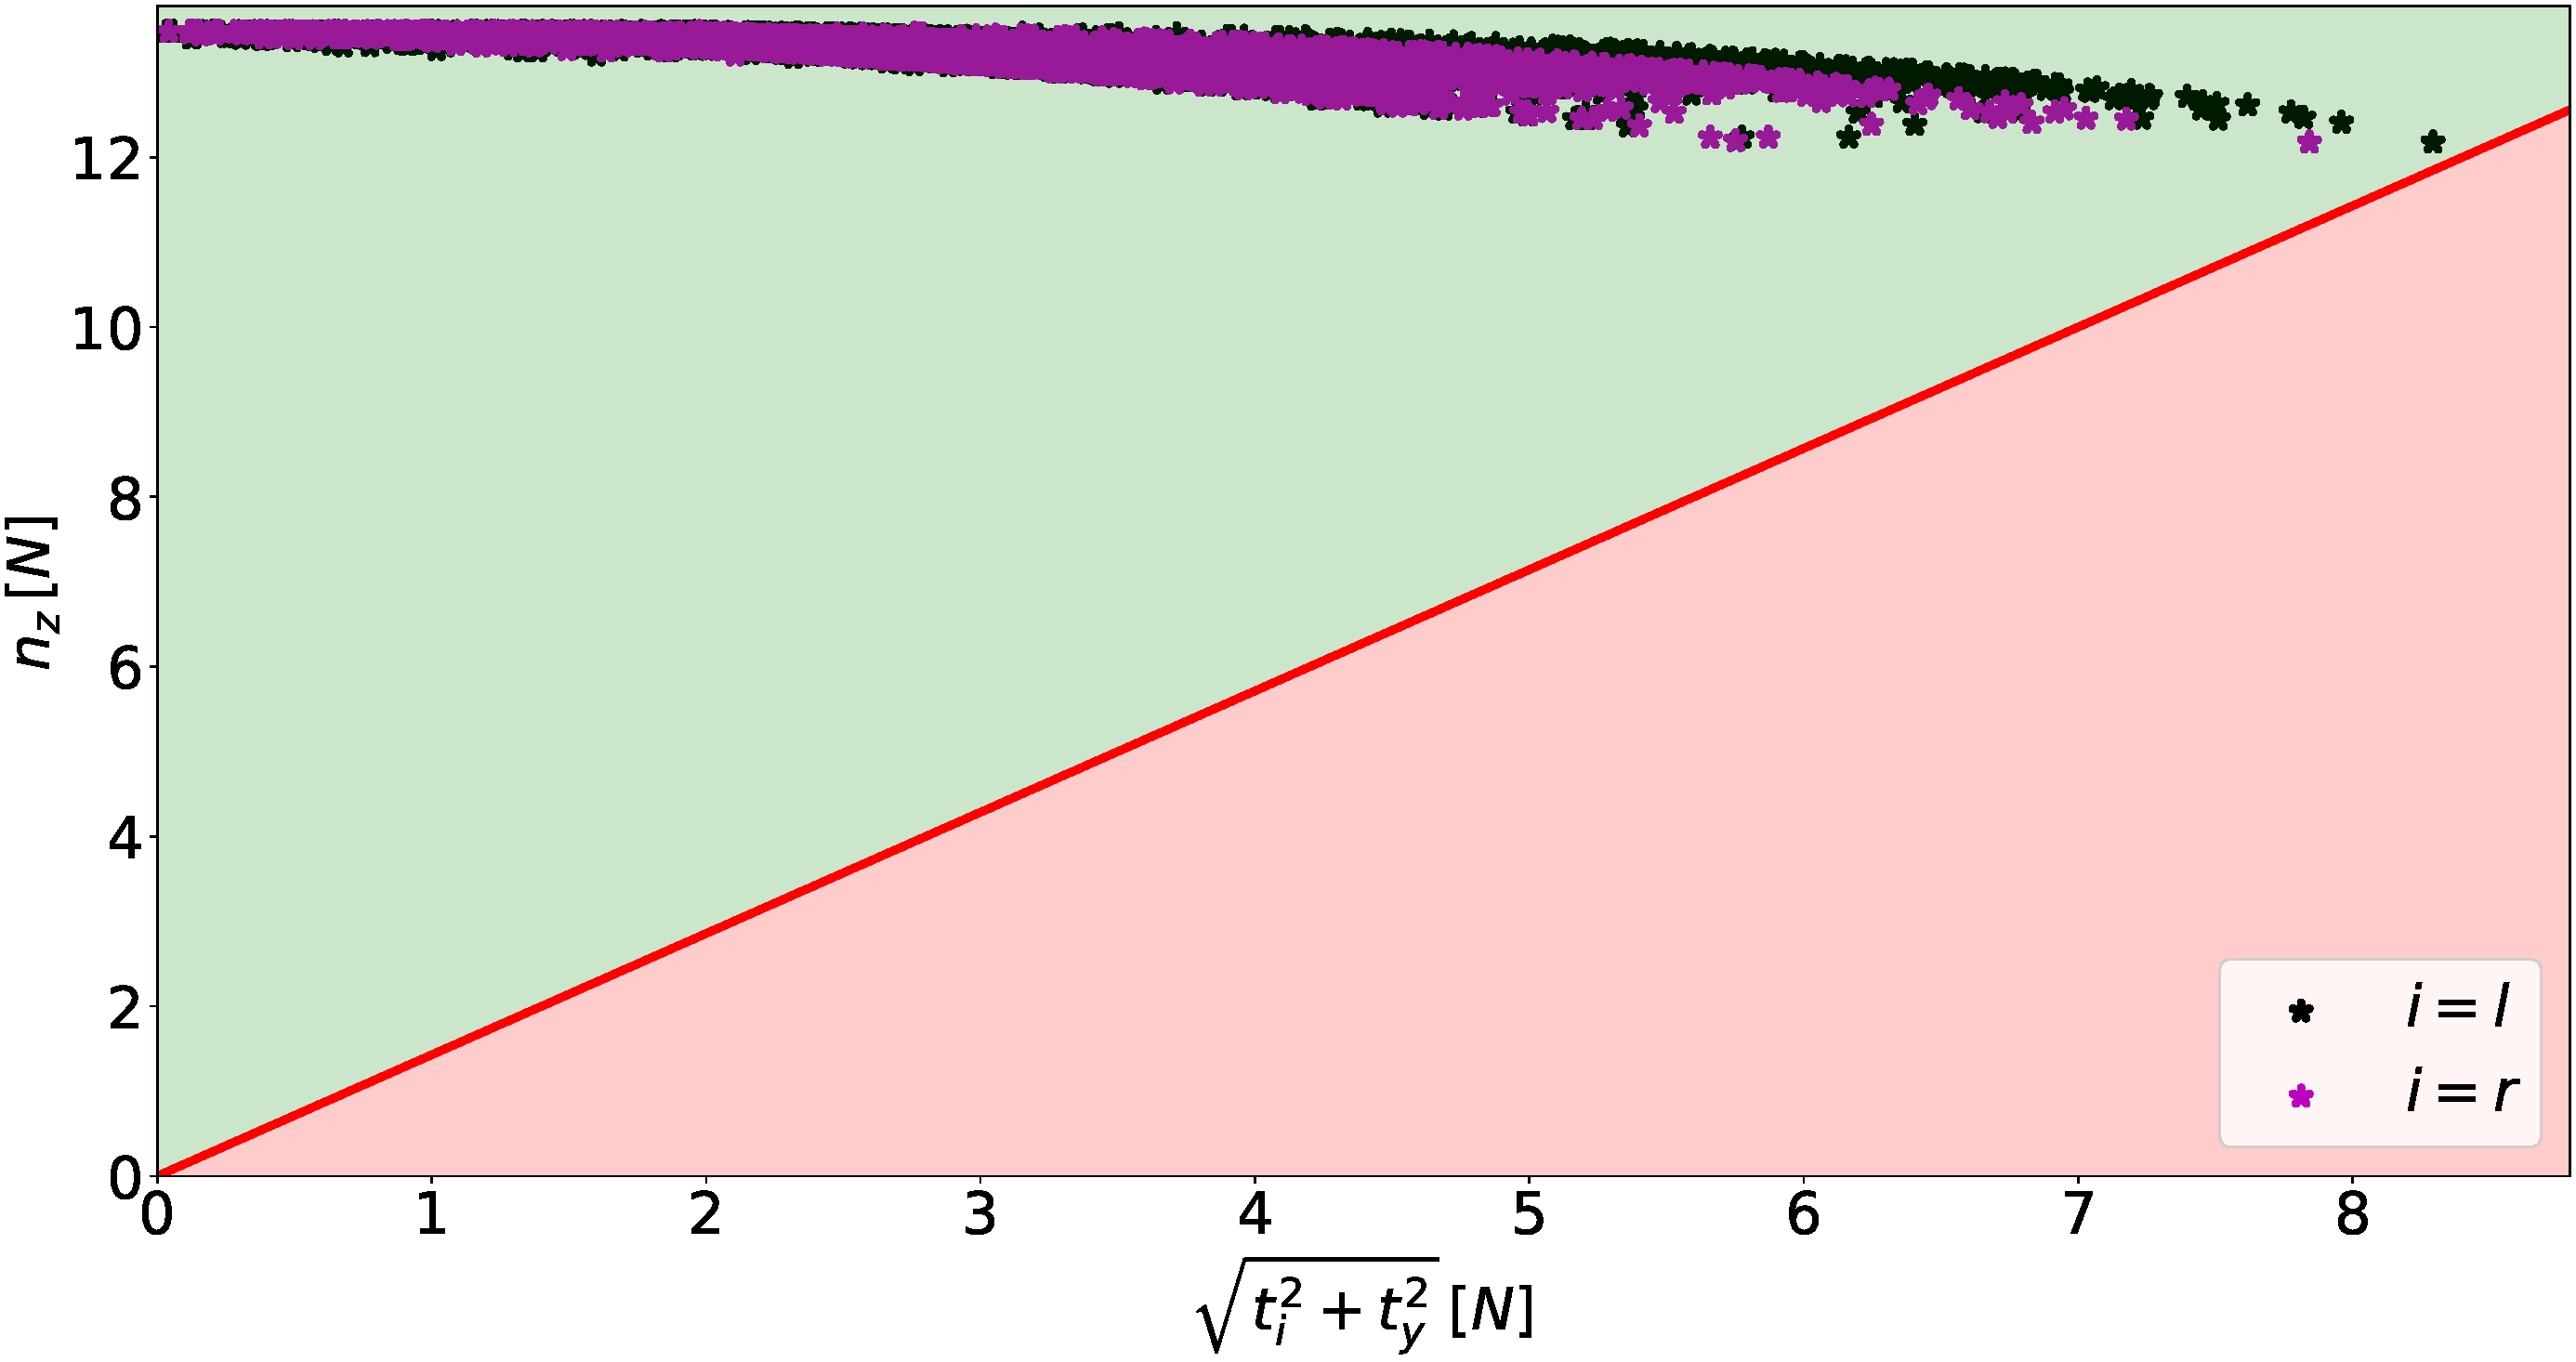
\includegraphics[width=0.325\linewidth]{Figures/Real time one stage OCP on rough terrain/Rough and uneven terrain map/forces_cone_tabgreen.pdf}}
    \subfigure[\textcolor{tabred}{Red}]{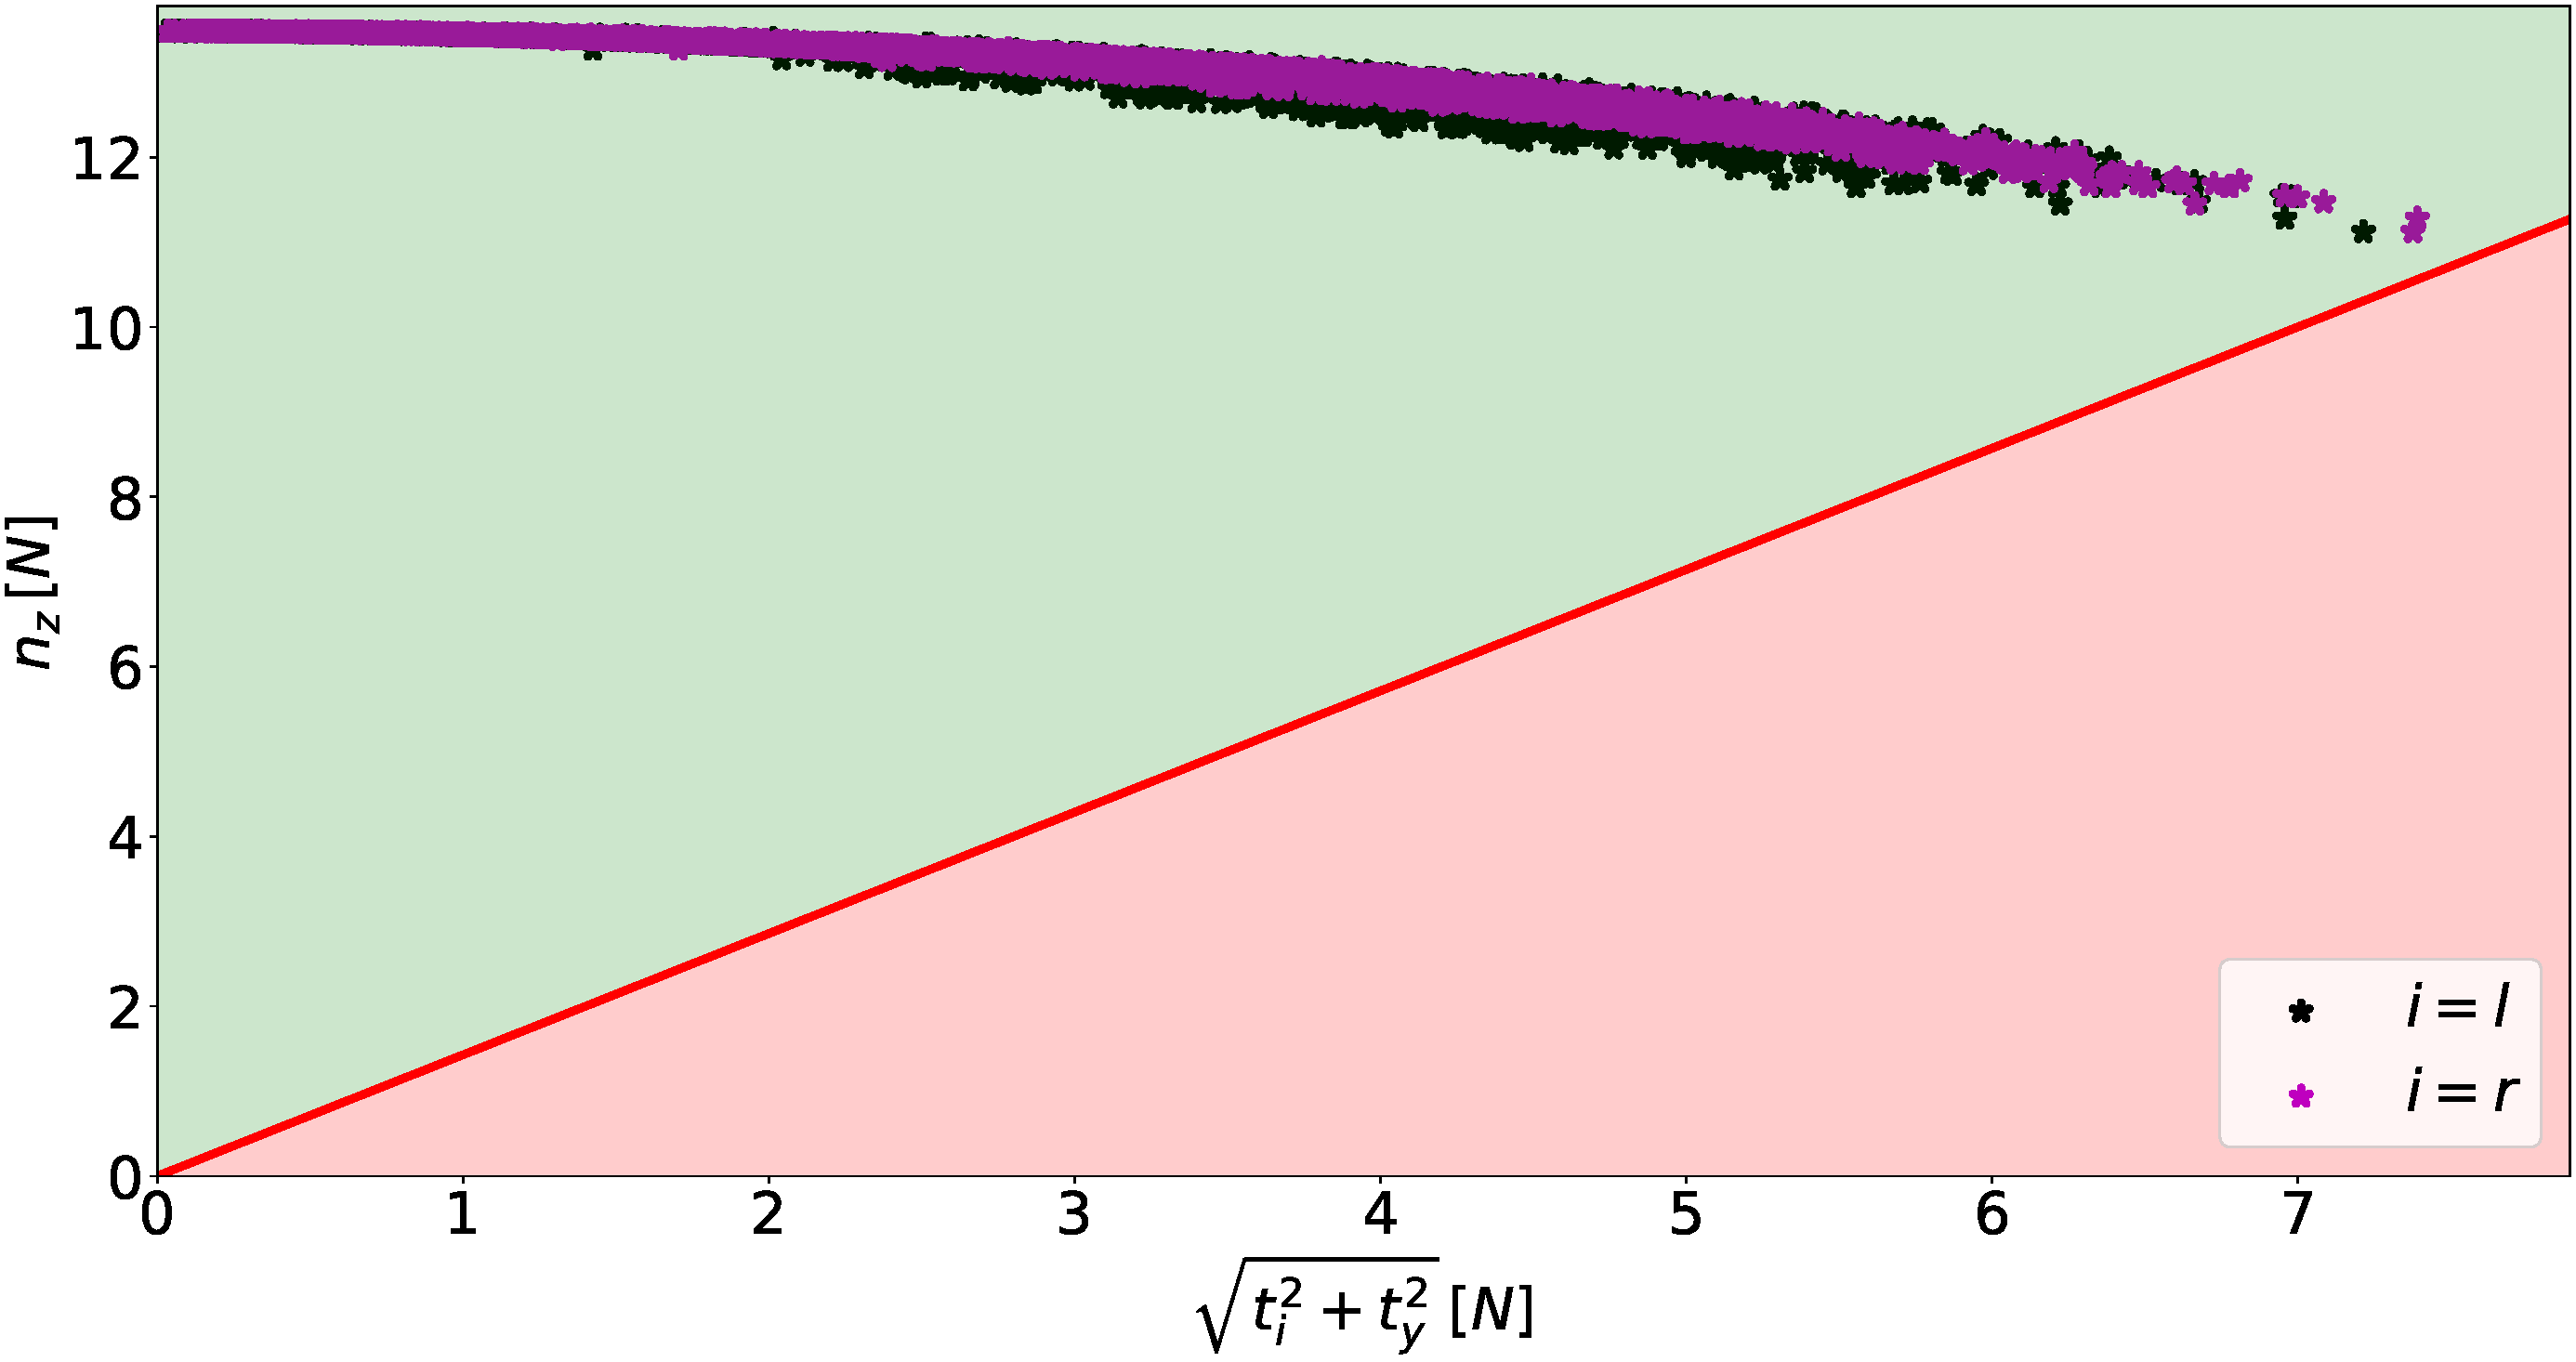
\includegraphics[width=0.325\linewidth]{Figures/Real time one stage OCP on rough terrain/Rough and uneven terrain map/forces_cone_tabred.pdf}}
    \subfigure[\textcolor{tabpurple}{Purple}]{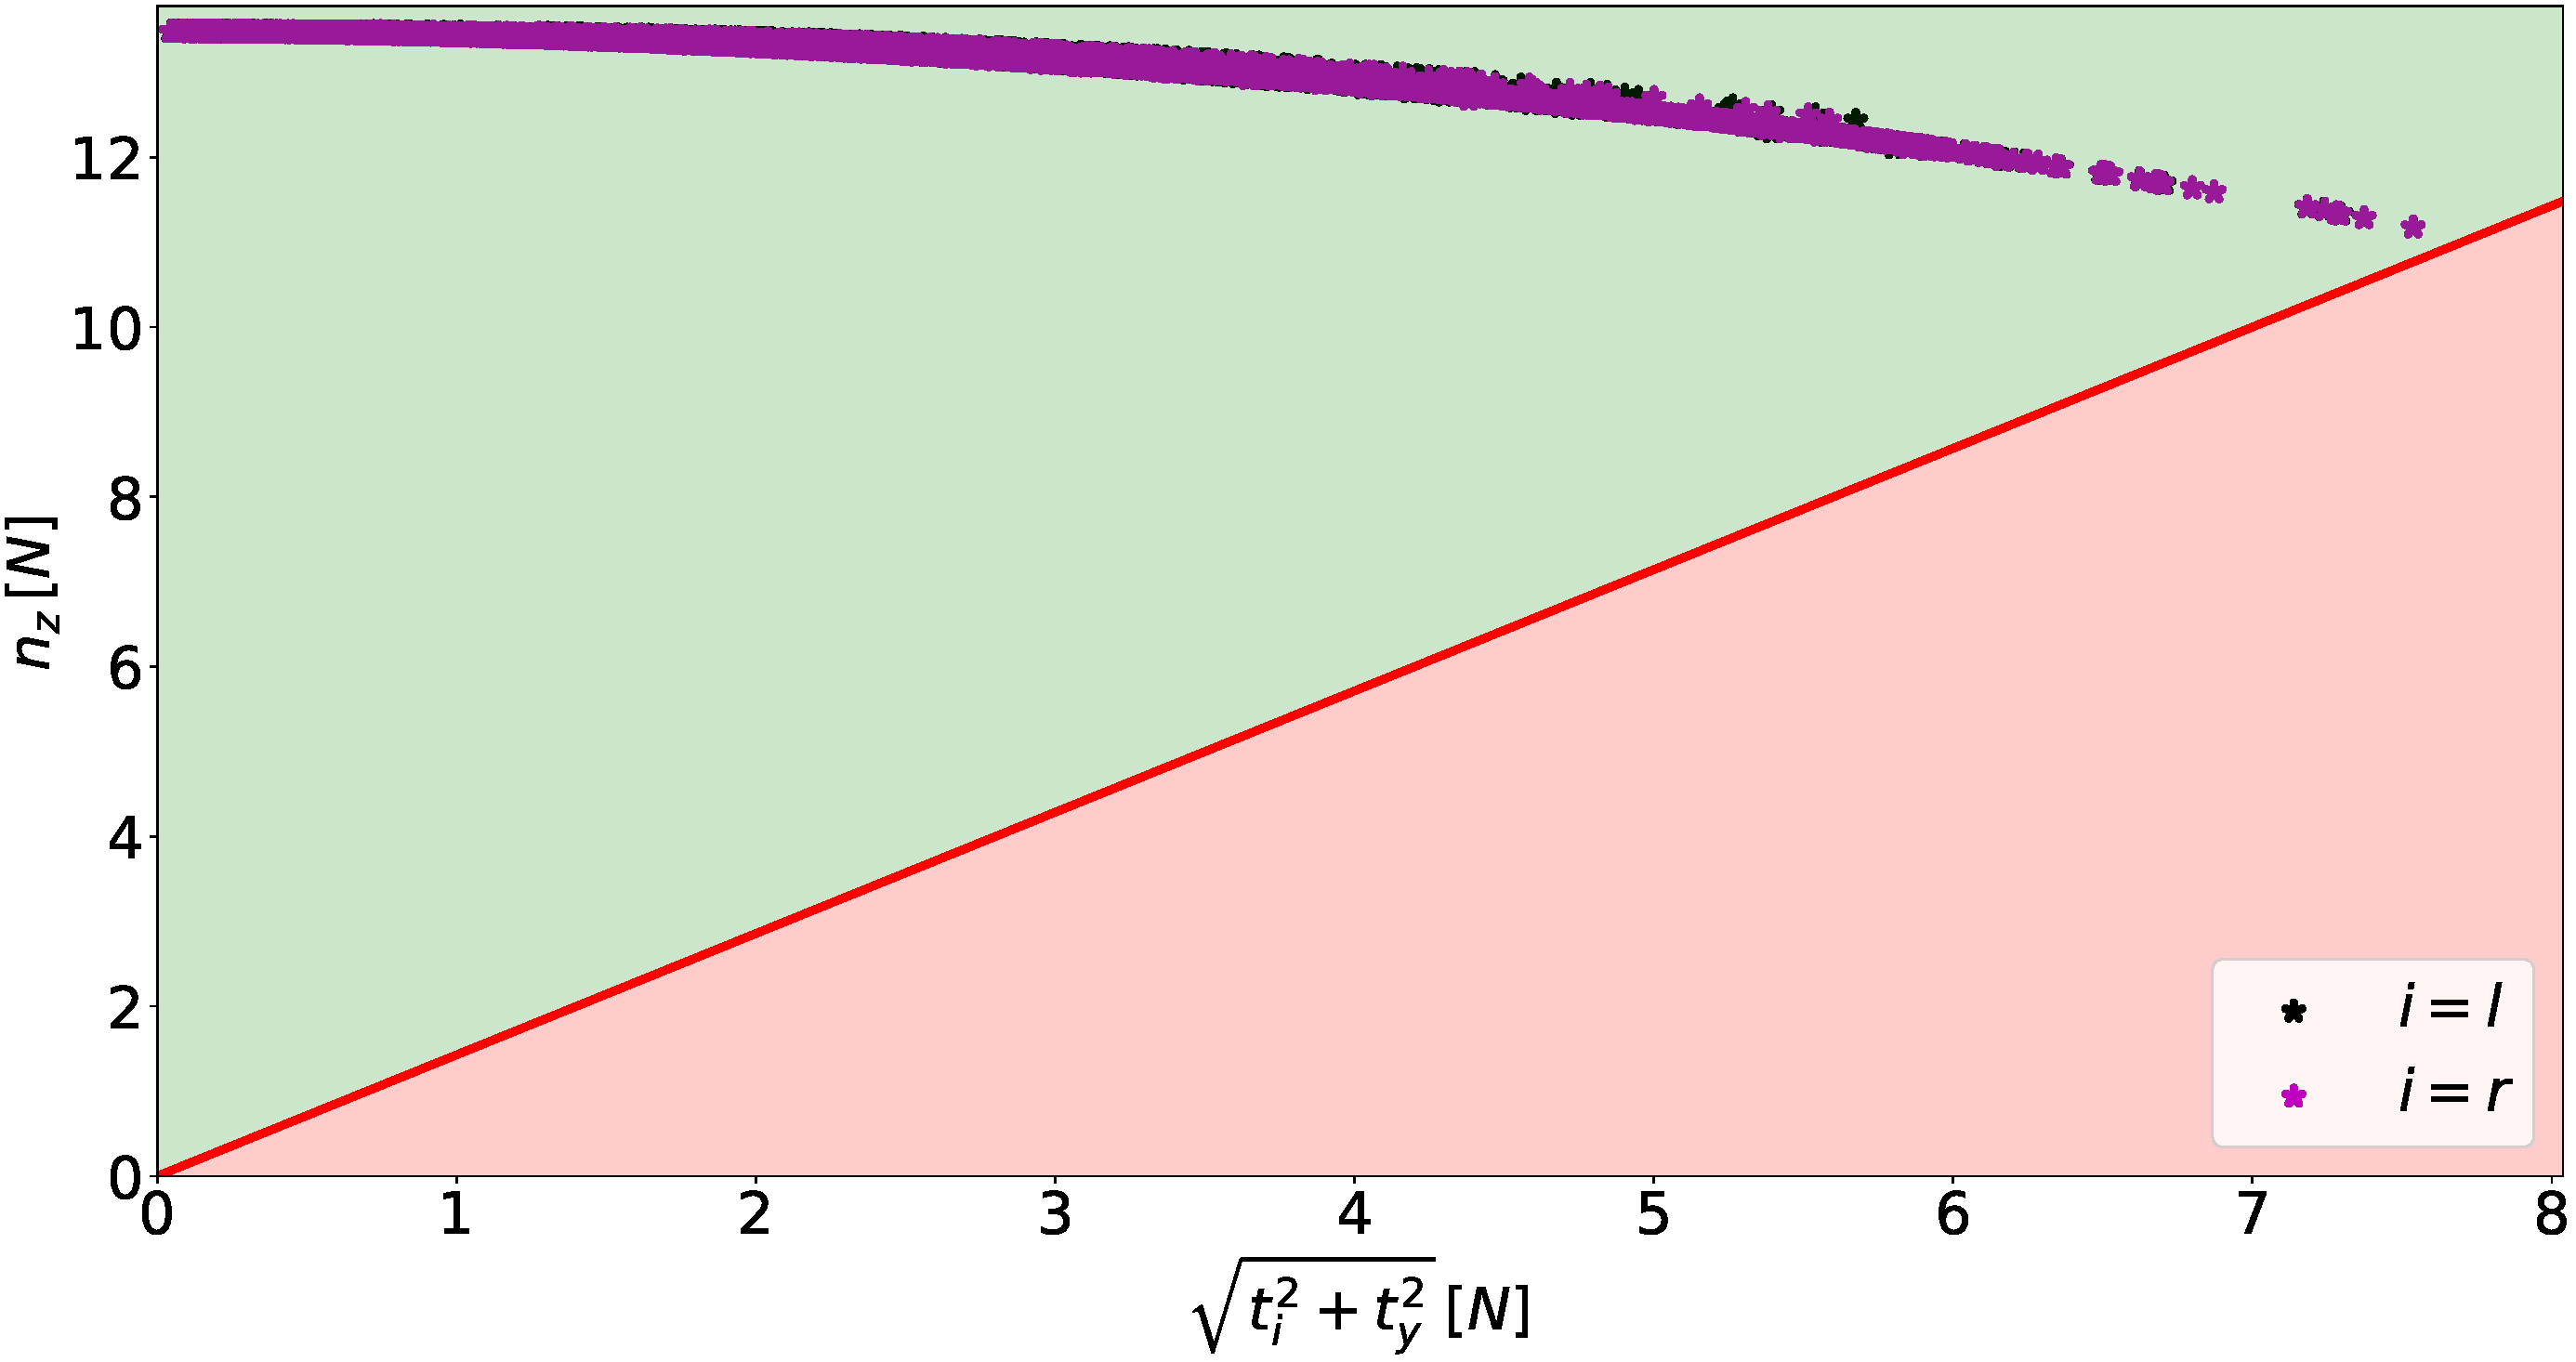
\includegraphics[width=0.325\linewidth]{Figures/Real time one stage OCP on rough terrain/Rough and uneven terrain map/forces_cone_tabpurple.pdf}}
    \subfigure[\textcolor{tabbrown}{Brown}]{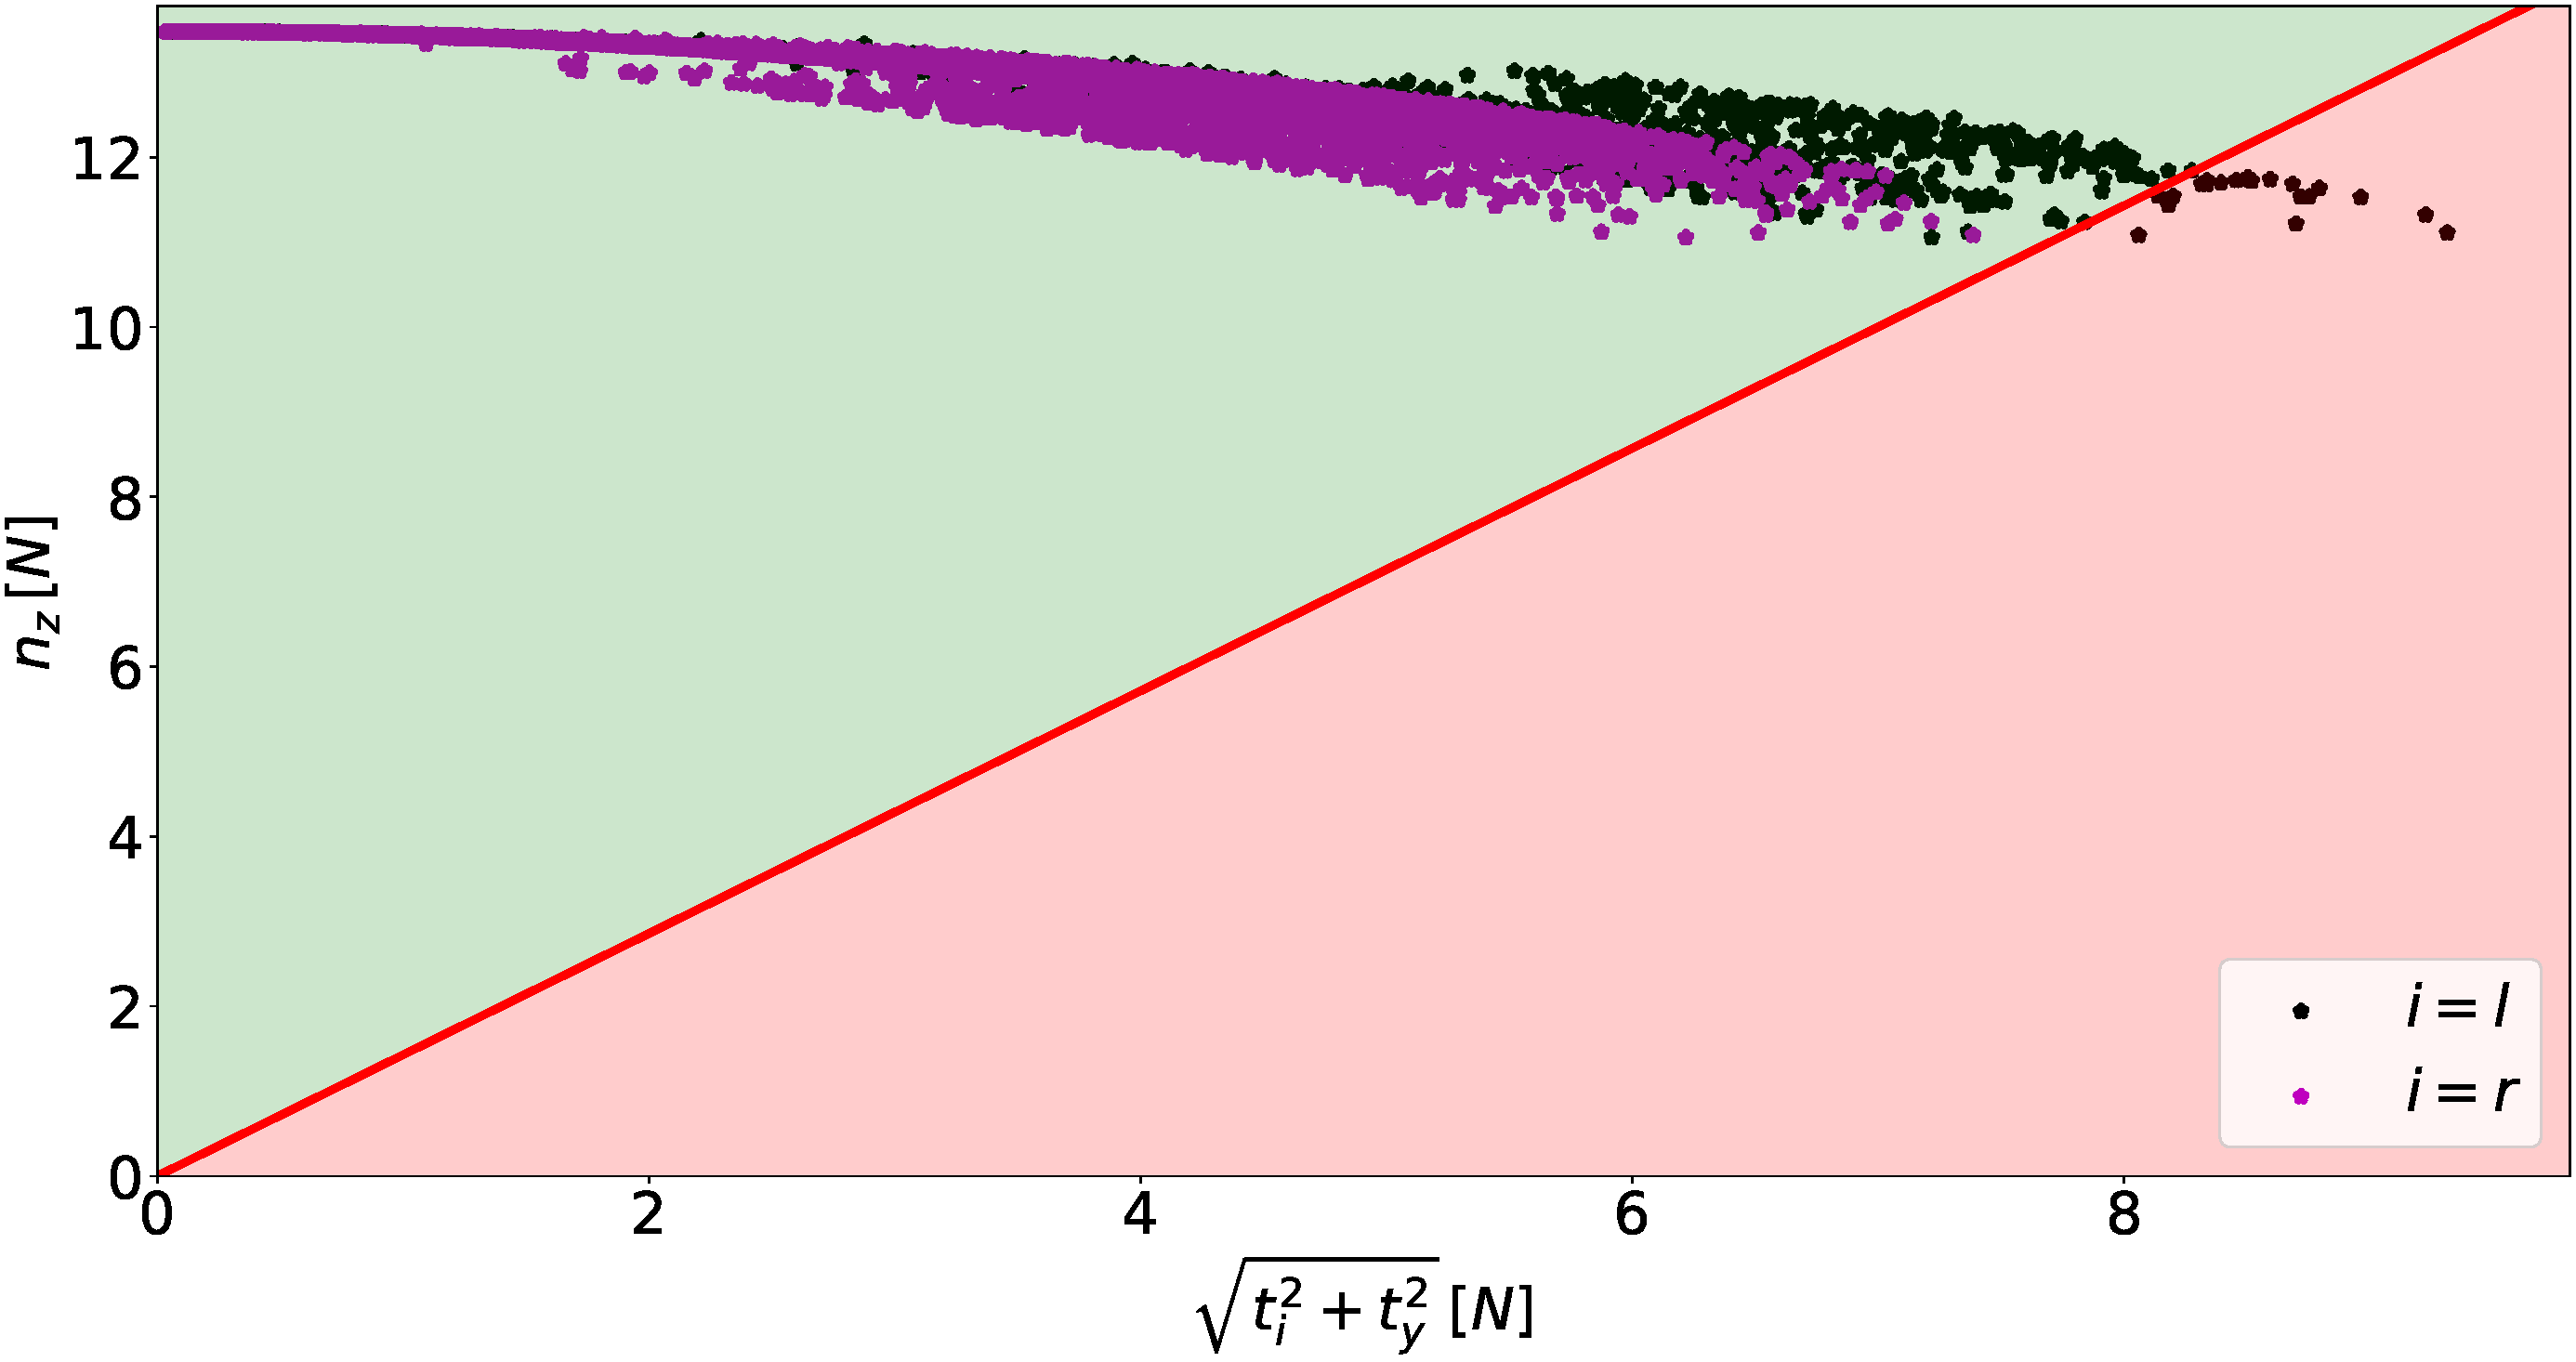
\includegraphics[width=0.325\linewidth]{Figures/Real time one stage OCP on rough terrain/Rough and uneven terrain map/forces_cone_tabbrown.pdf}}
    \subfigure[\textcolor{tabpink}{Pink}]{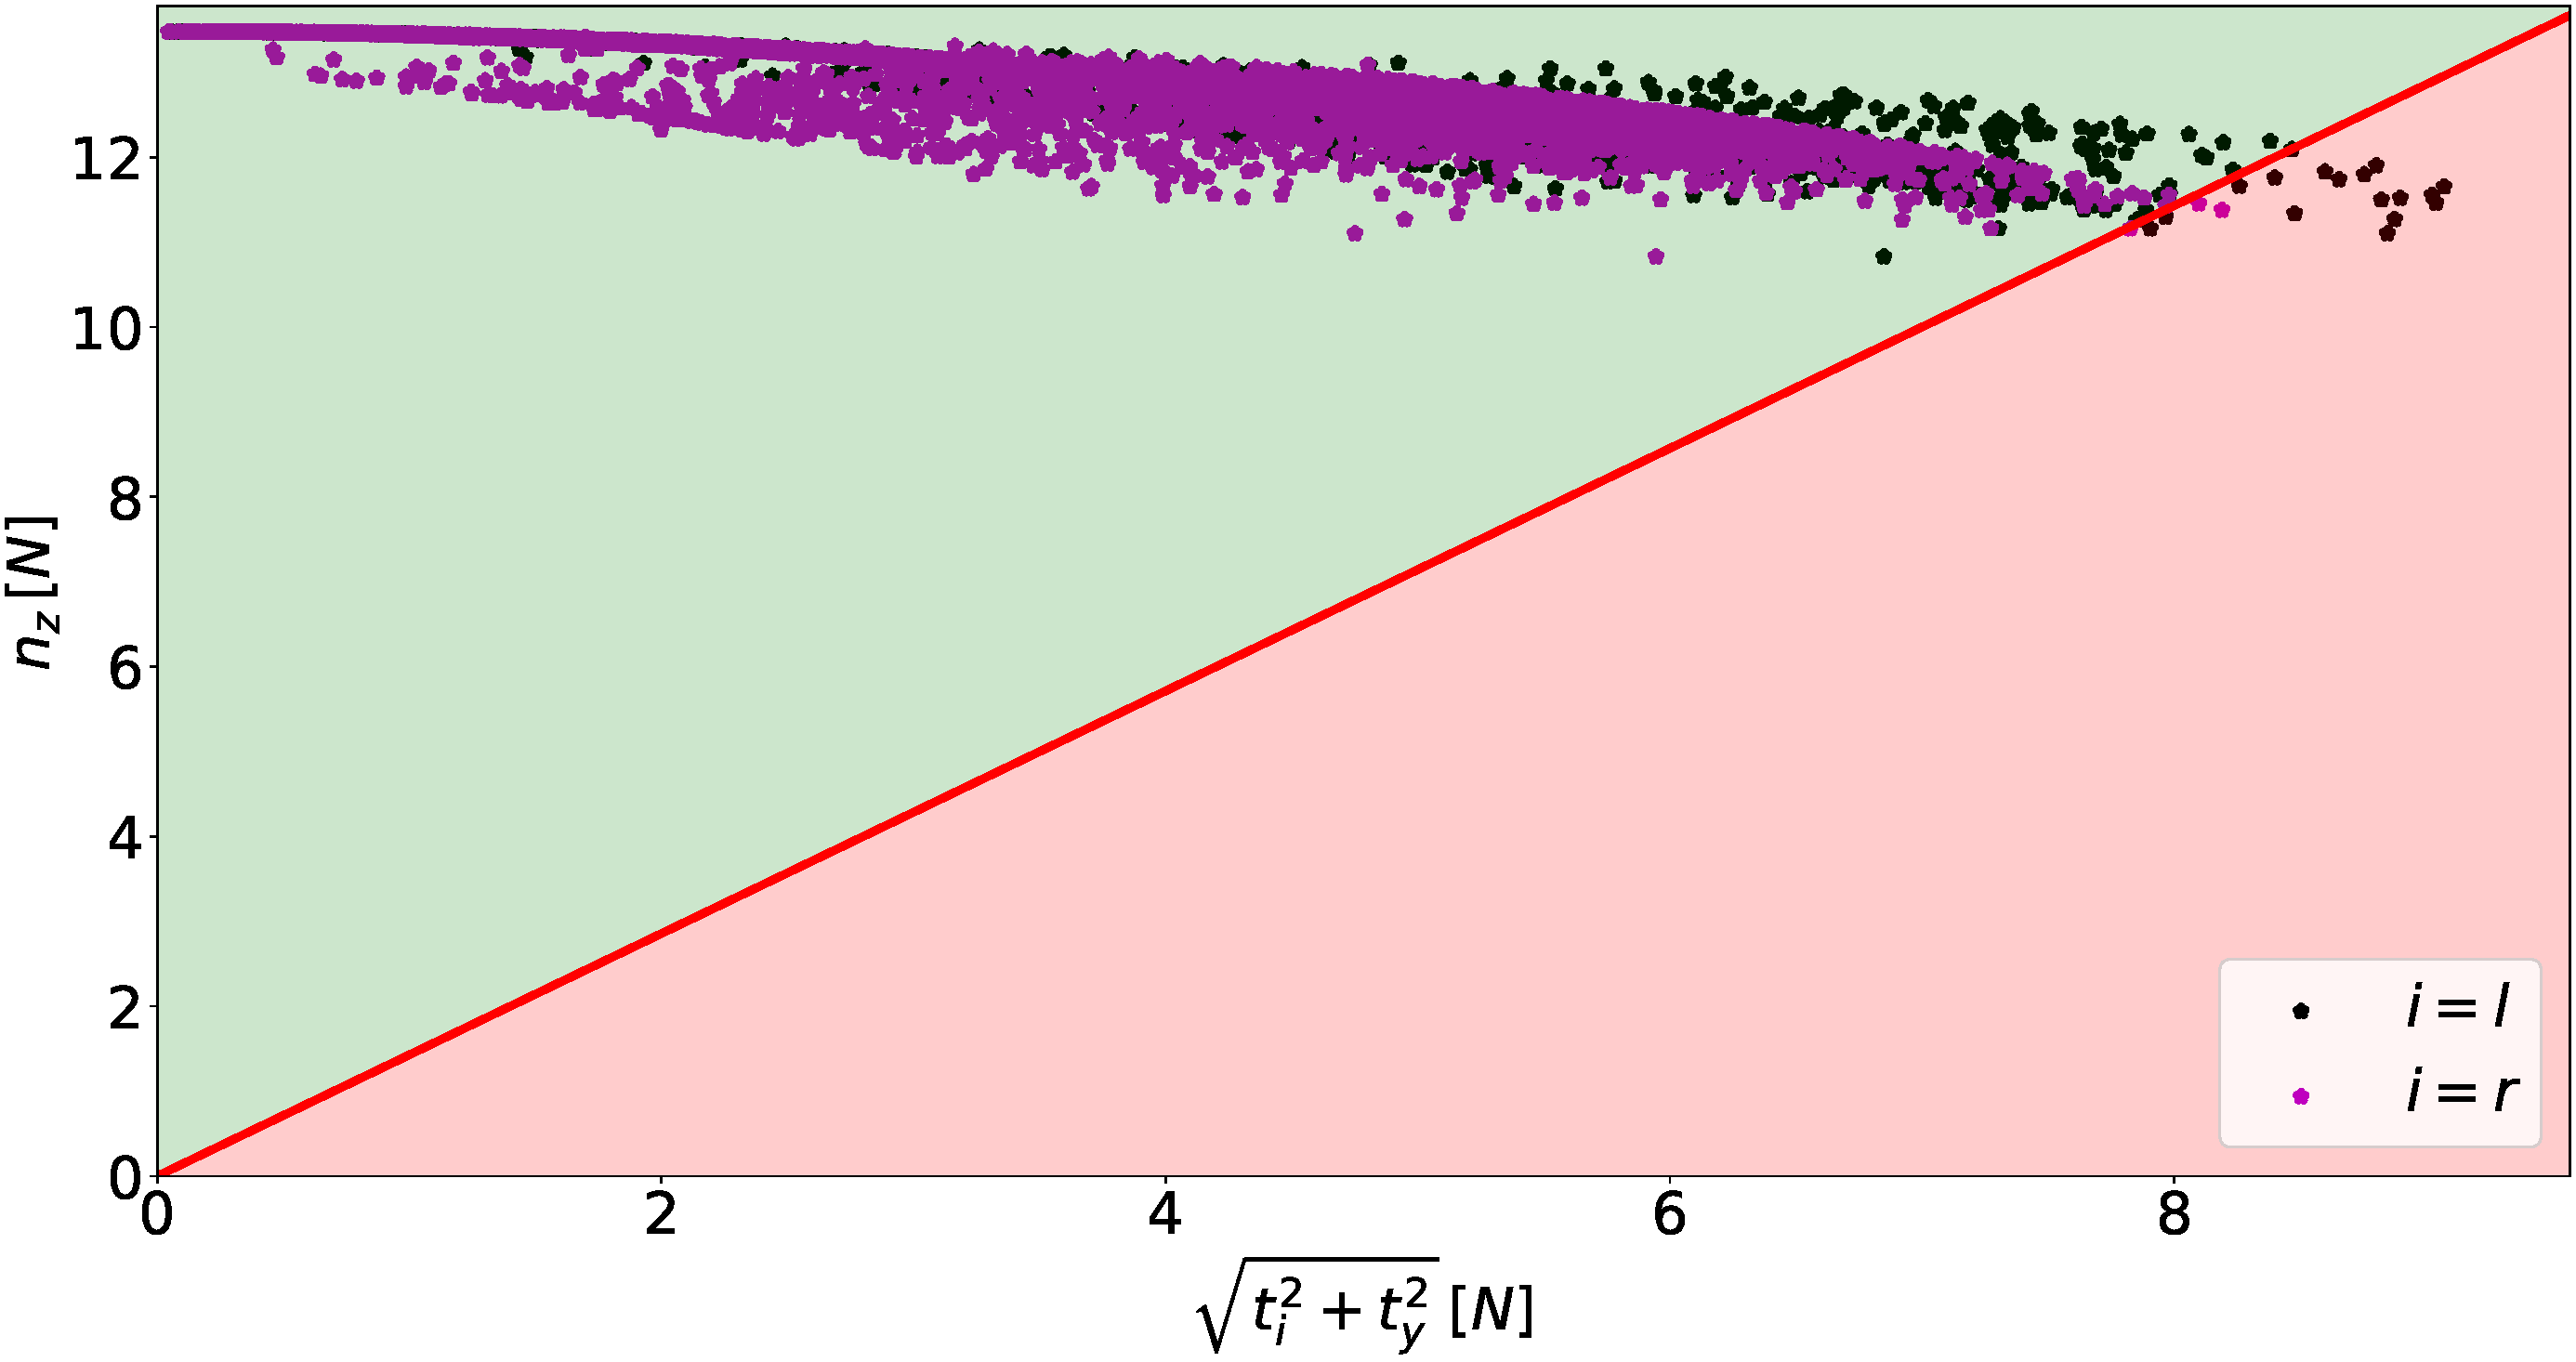
\includegraphics[width=0.325\linewidth]{Figures/Real time one stage OCP on rough terrain/Rough and uneven terrain map/forces_cone_tabpink.pdf}}
    \subfigure[\textcolor{tabgray}{Gray}]{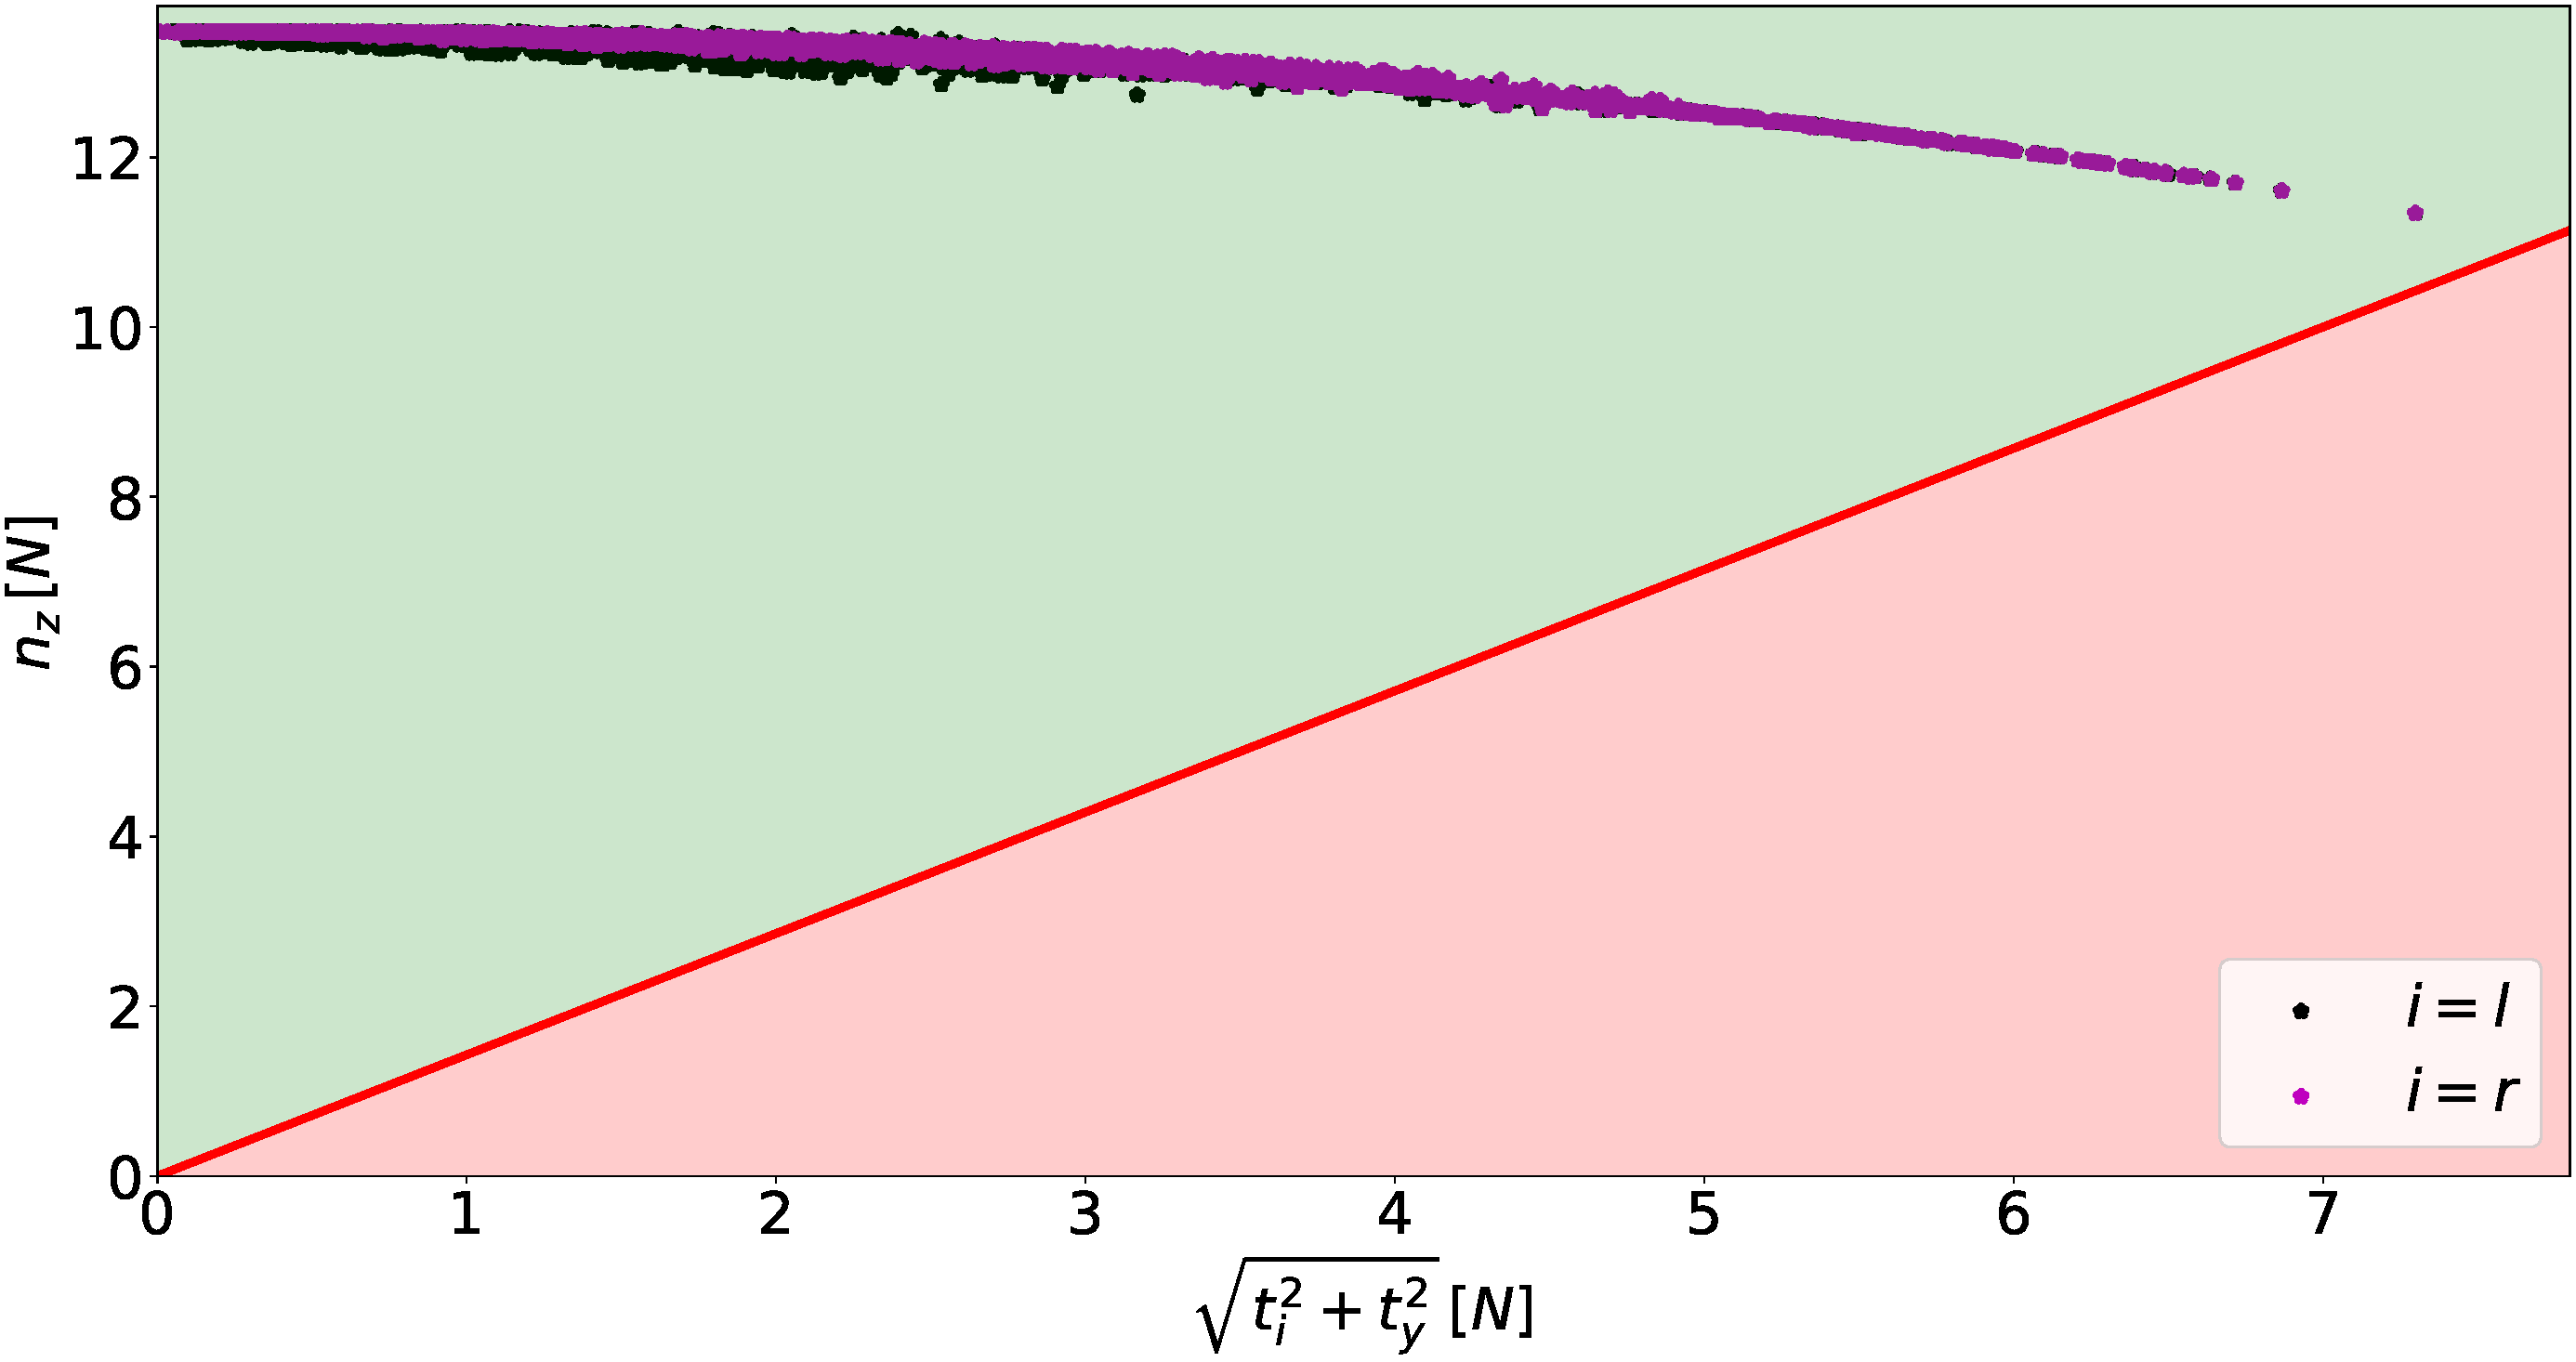
\includegraphics[width=0.325\linewidth]{Figures/Real time one stage OCP on rough terrain/Rough and uneven terrain map/forces_cone_tabgray.pdf}}
    \subfigure[\textcolor{tabolive}{Olive}]{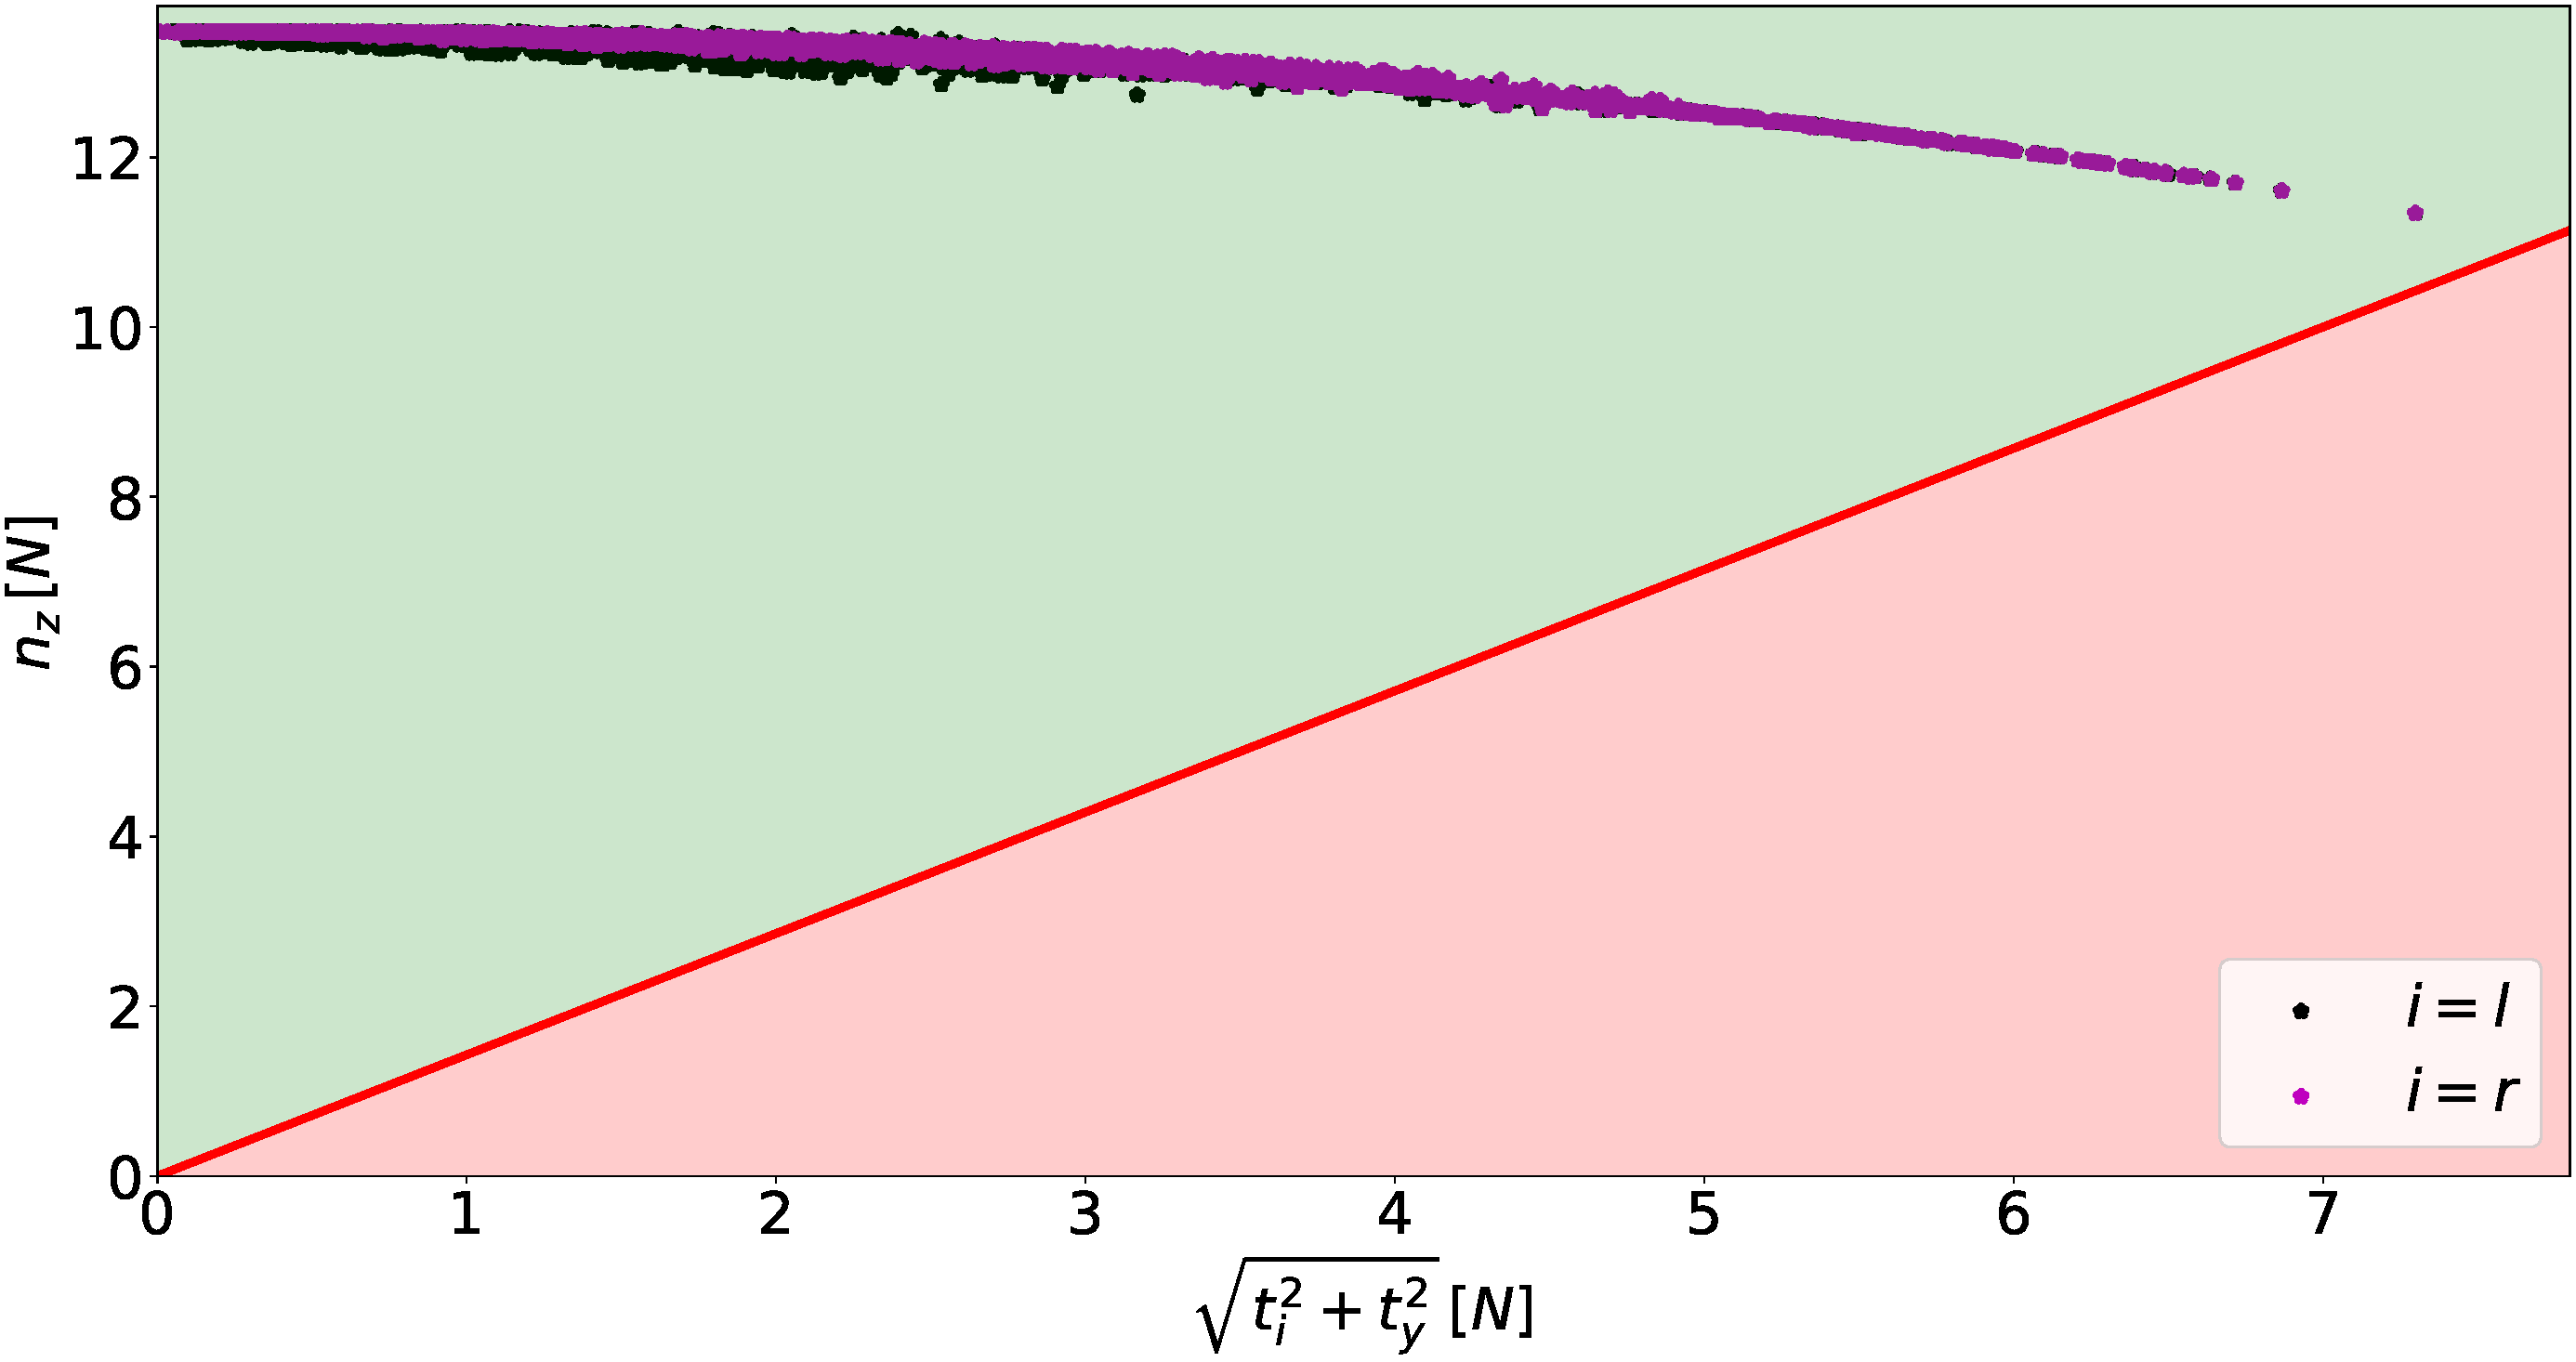
\includegraphics[width=0.325\linewidth]{Figures/Real time one stage OCP on rough terrain/Rough and uneven terrain map/forces_cone_tabgray.pdf}}
  \end{subfigmatrix}
  \caption{Coulomb traction forces cone.}
  \label{fig:RoughUnevenTerrainForcesConeStartAway}
\end{figure}

\subsubsection*{Robustness tests}

To end this chapter, solver \ti{Low rate of change} is subject to the same robustness test that was described in \ref{subsection:realTimeOneStagePlanarOCP}. This time, only set $\x,\,\y \sim \mathcal{N}\left(0.0,\,0.01\right),\; \yaw\sim\mathcal{N}\left(0.0,\,0.001\right)$ of white gaussian noise was applied. The complete tour of the reference is performed, and $100000$ iterations were recorded.

Figure \ref{fig:robustnessResultsSolver3} assembles all the relevant results of this test. Once more, solver \ti{Low rate of change} has proven to be computationally feasible. The recorded optimal time and costs were $(5.31) \pm (1.01)\,[ms]$ and $(20.81) \pm (31.19)$, respectively. Slippage occurs $0.09 \%$ and the solver fails on $0.03 \%$ of the iterations.

Even in the face of disturbances, the solver is able to keep the mobile robot on track, in spite of the significant deviations that noise inflicts. Slippage is rare and the traction rates are roughly kept in the interval $[-5,\,5]\,[N \cdot s]$, which shows that the solver engages on a moderate change of forces.  The velocities are also kept within a safe interval, so that the mobile robot does not reach fast (and unsafe) velocities, mainly due to the low virtual reference speed.

\begin{figure}[!htb]
  \begin{subfigmatrix}{4}
    \subfigure[Optimal cost along path tracking.]{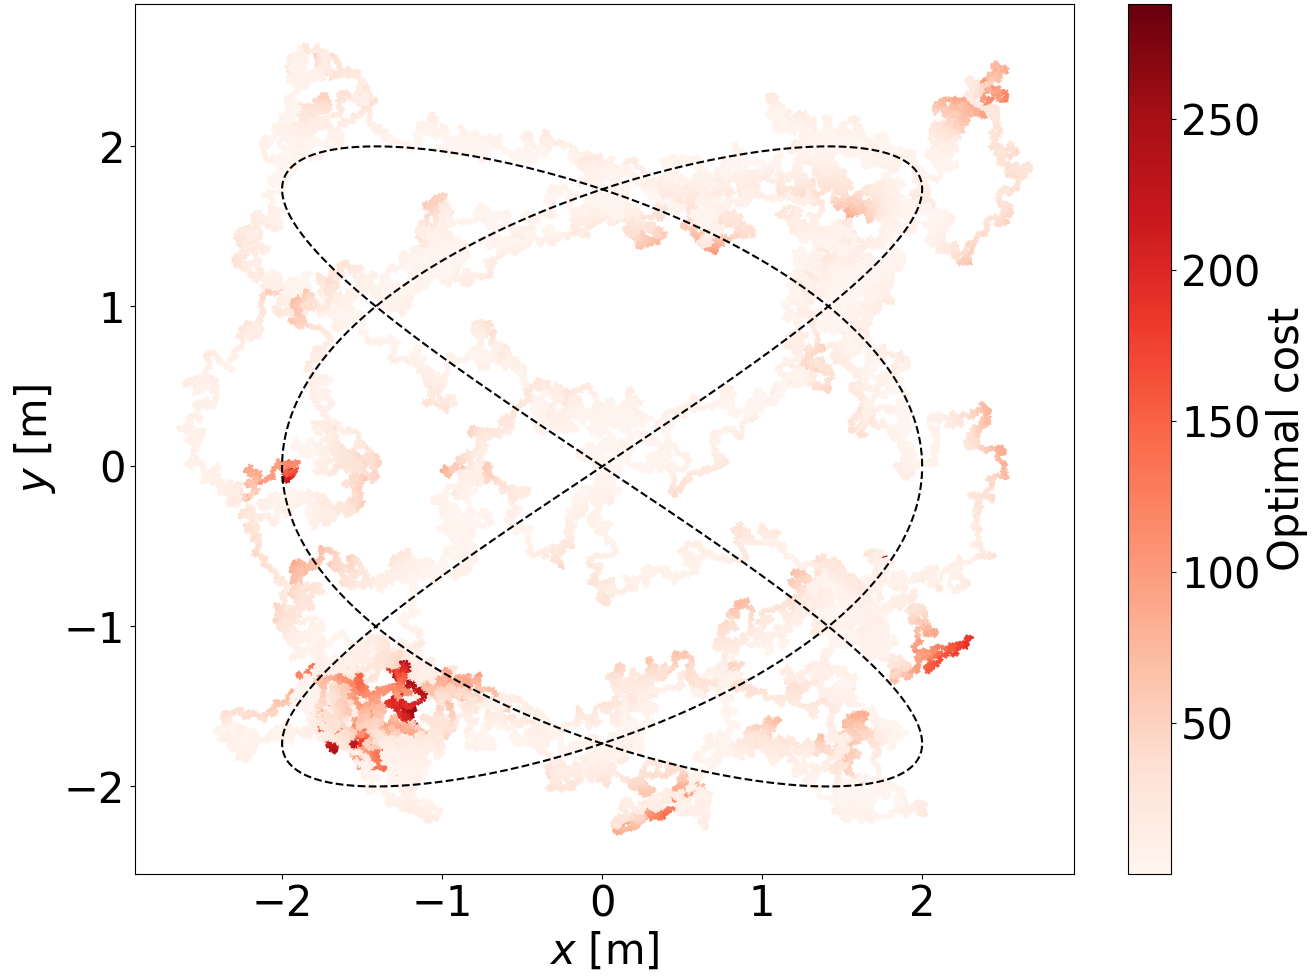
\includegraphics[width=0.49\linewidth]{Figures/Real time one stage OCP on rough terrain/Robustness tests/path_tracking_optimal_cost.png}}
    \subfigure[Optimal time along path tracking.]{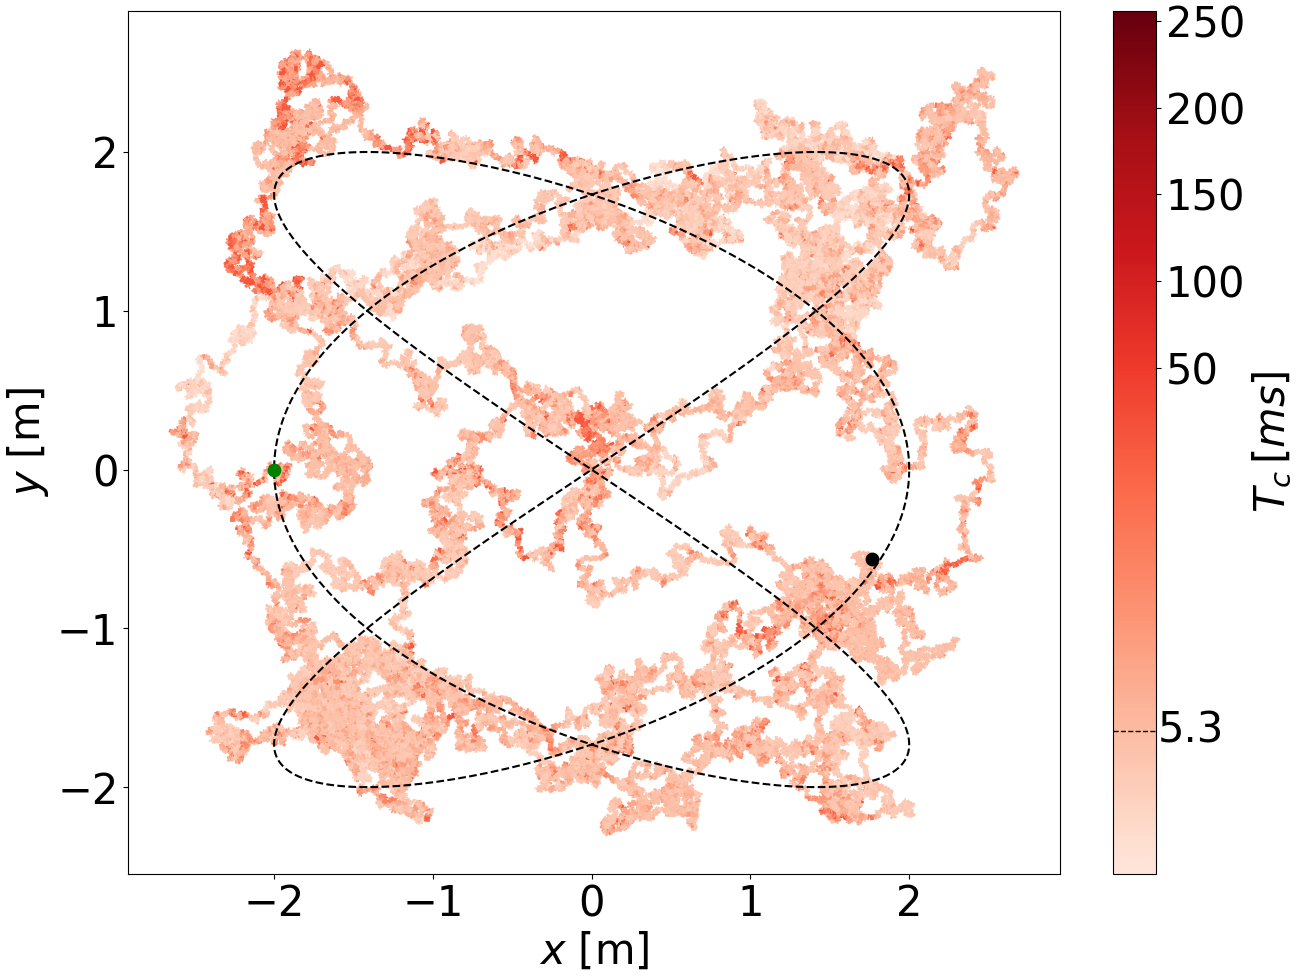
\includegraphics[width=0.49\linewidth]{Figures/Real time one stage OCP on rough terrain/Robustness tests/path_tracking_optimal_time.png}}
    \subfigure[Yaw curve.]{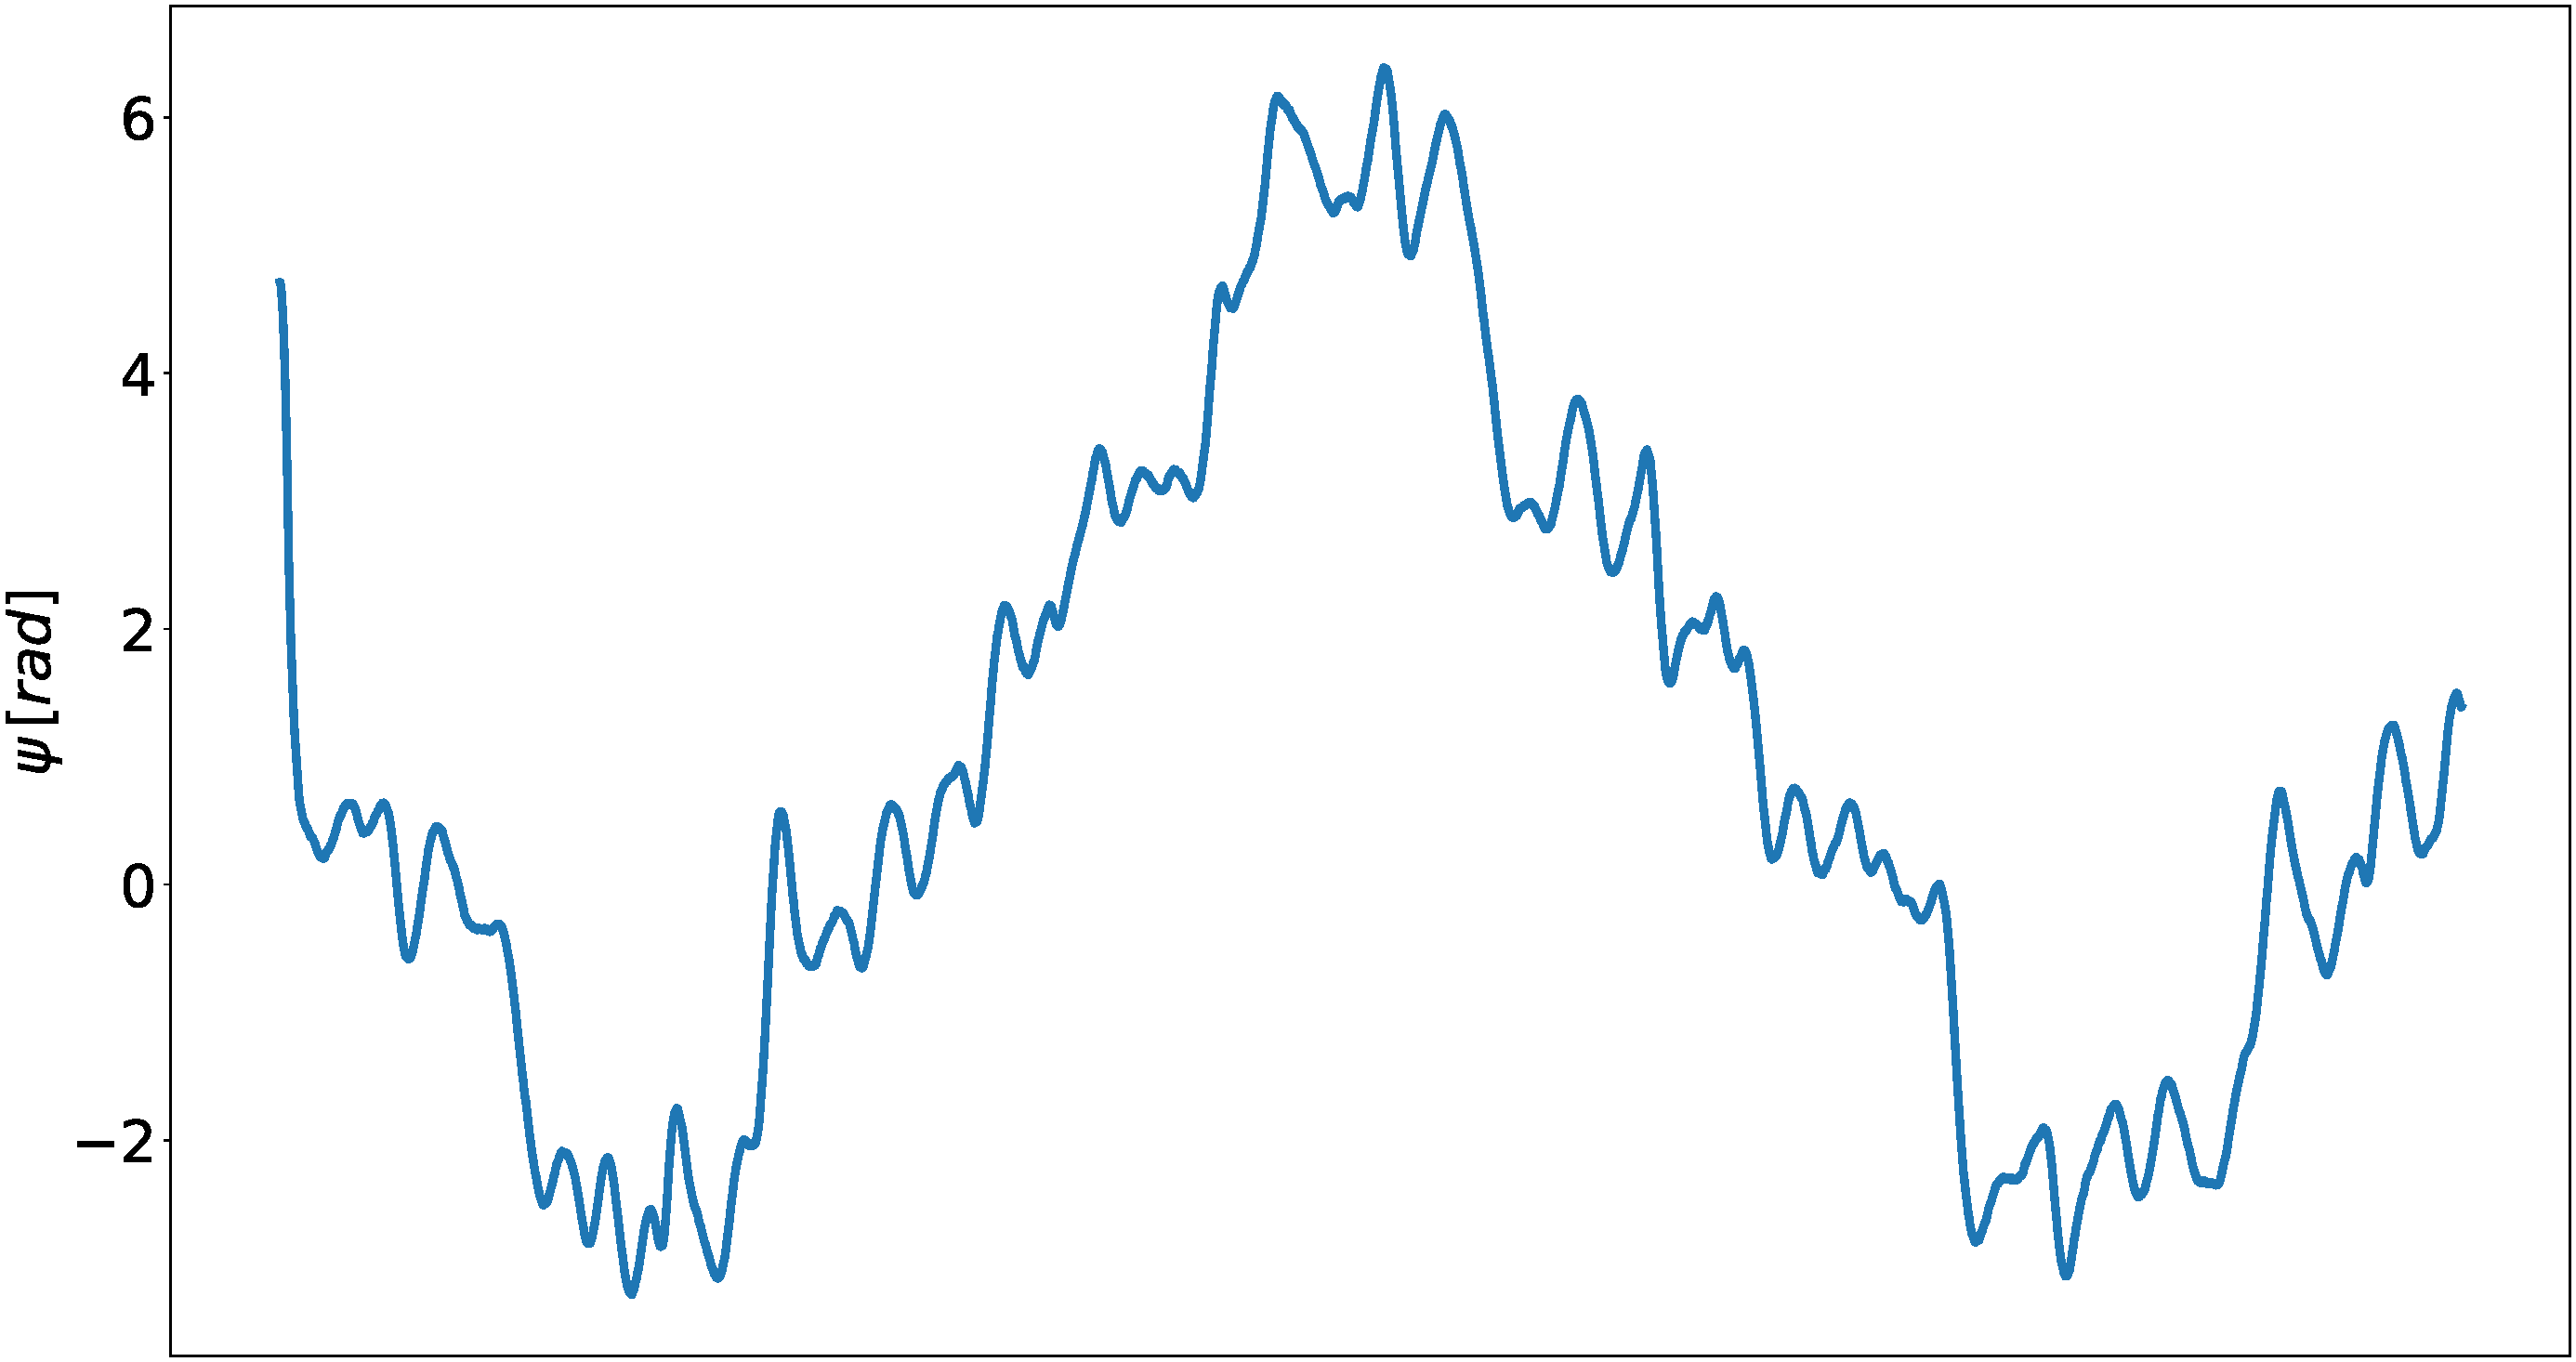
\includegraphics[width=0.49\linewidth]{Figures/Real time one stage OCP on rough terrain/Robustness tests/yaw_curve.pdf}}
    \subfigure[Traction forces on friction cone.]{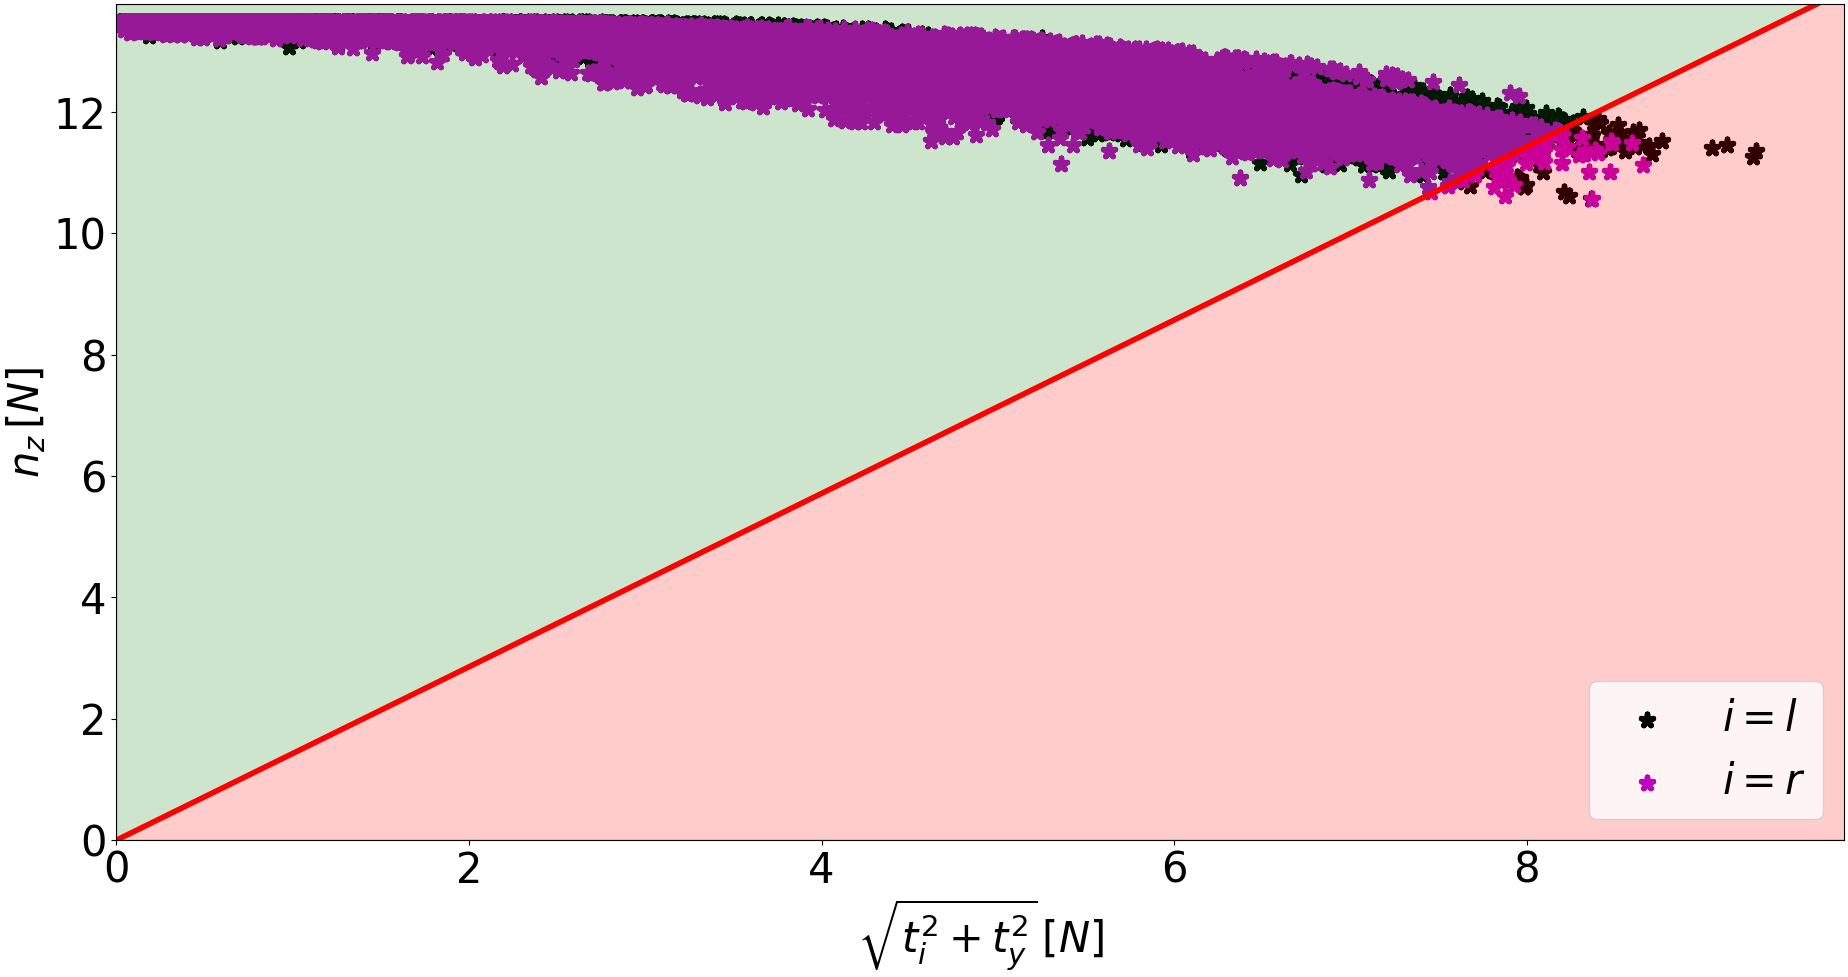
\includegraphics[width=0.49\linewidth]{Figures/Real time one stage OCP on rough terrain/Robustness tests/forces_cone.png}}
    \subfigure[Linear and angular velocity curves.]{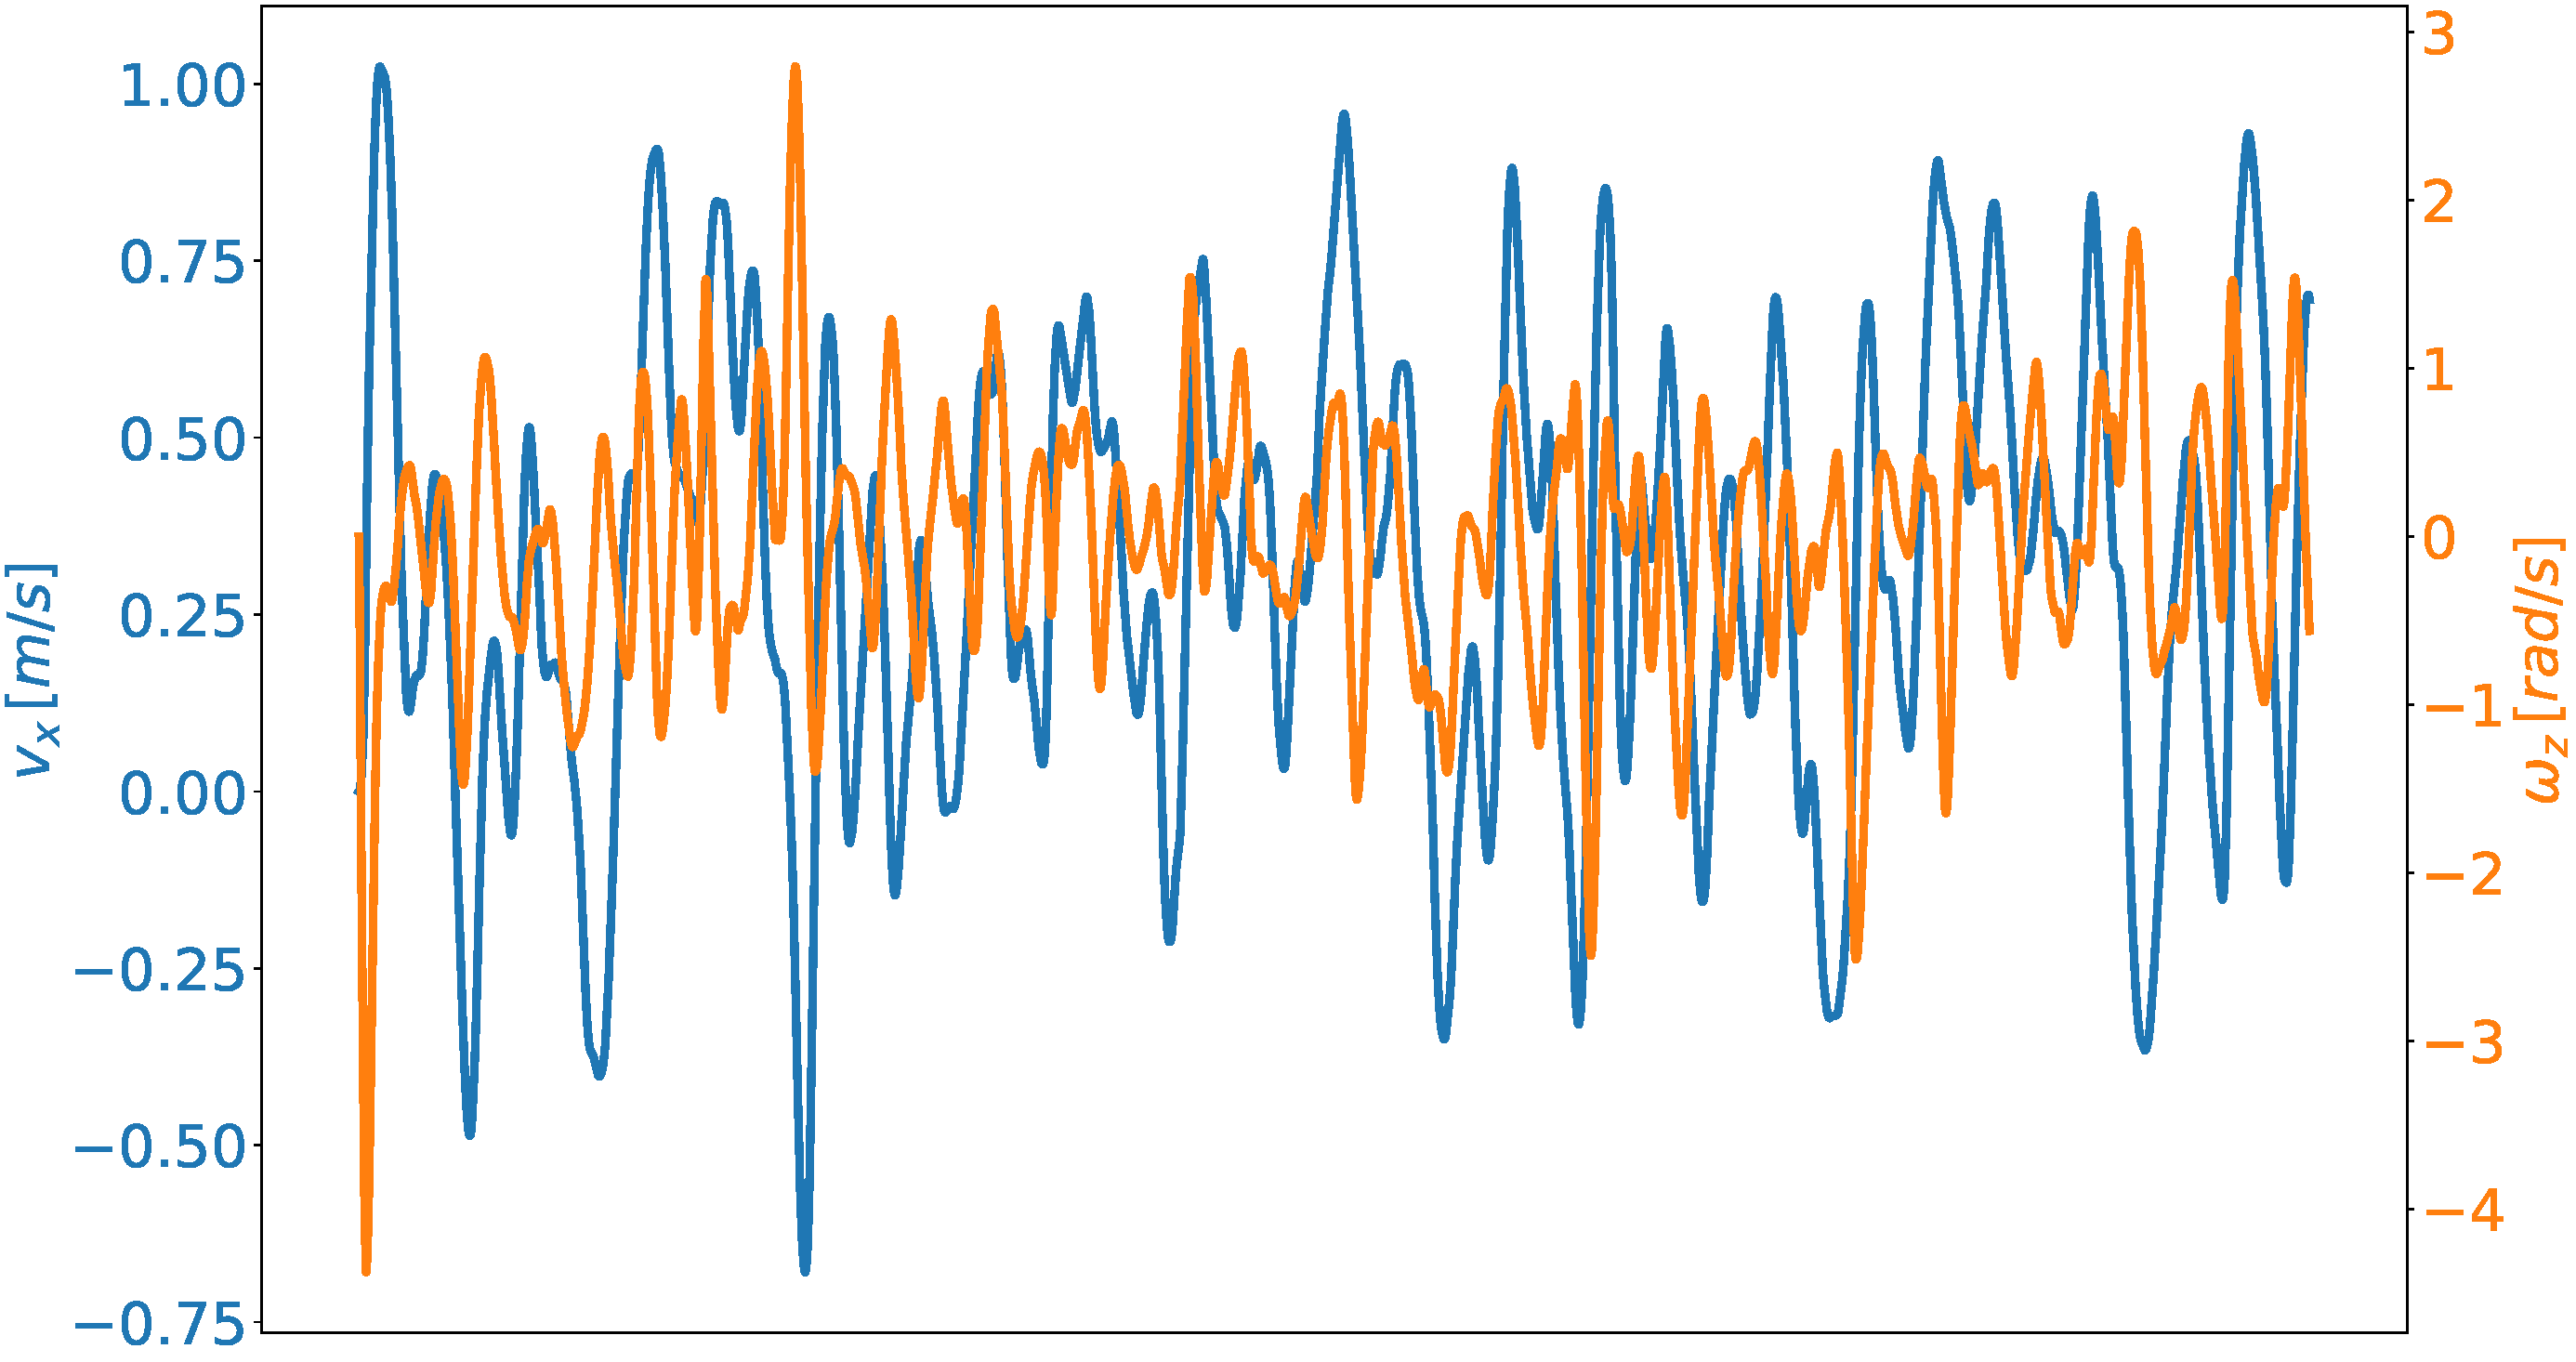
\includegraphics[width=0.49\linewidth]{Figures/Real time one stage OCP on rough terrain/Robustness tests/velocities_curves.pdf}}
    \subfigure[Traction rates.]{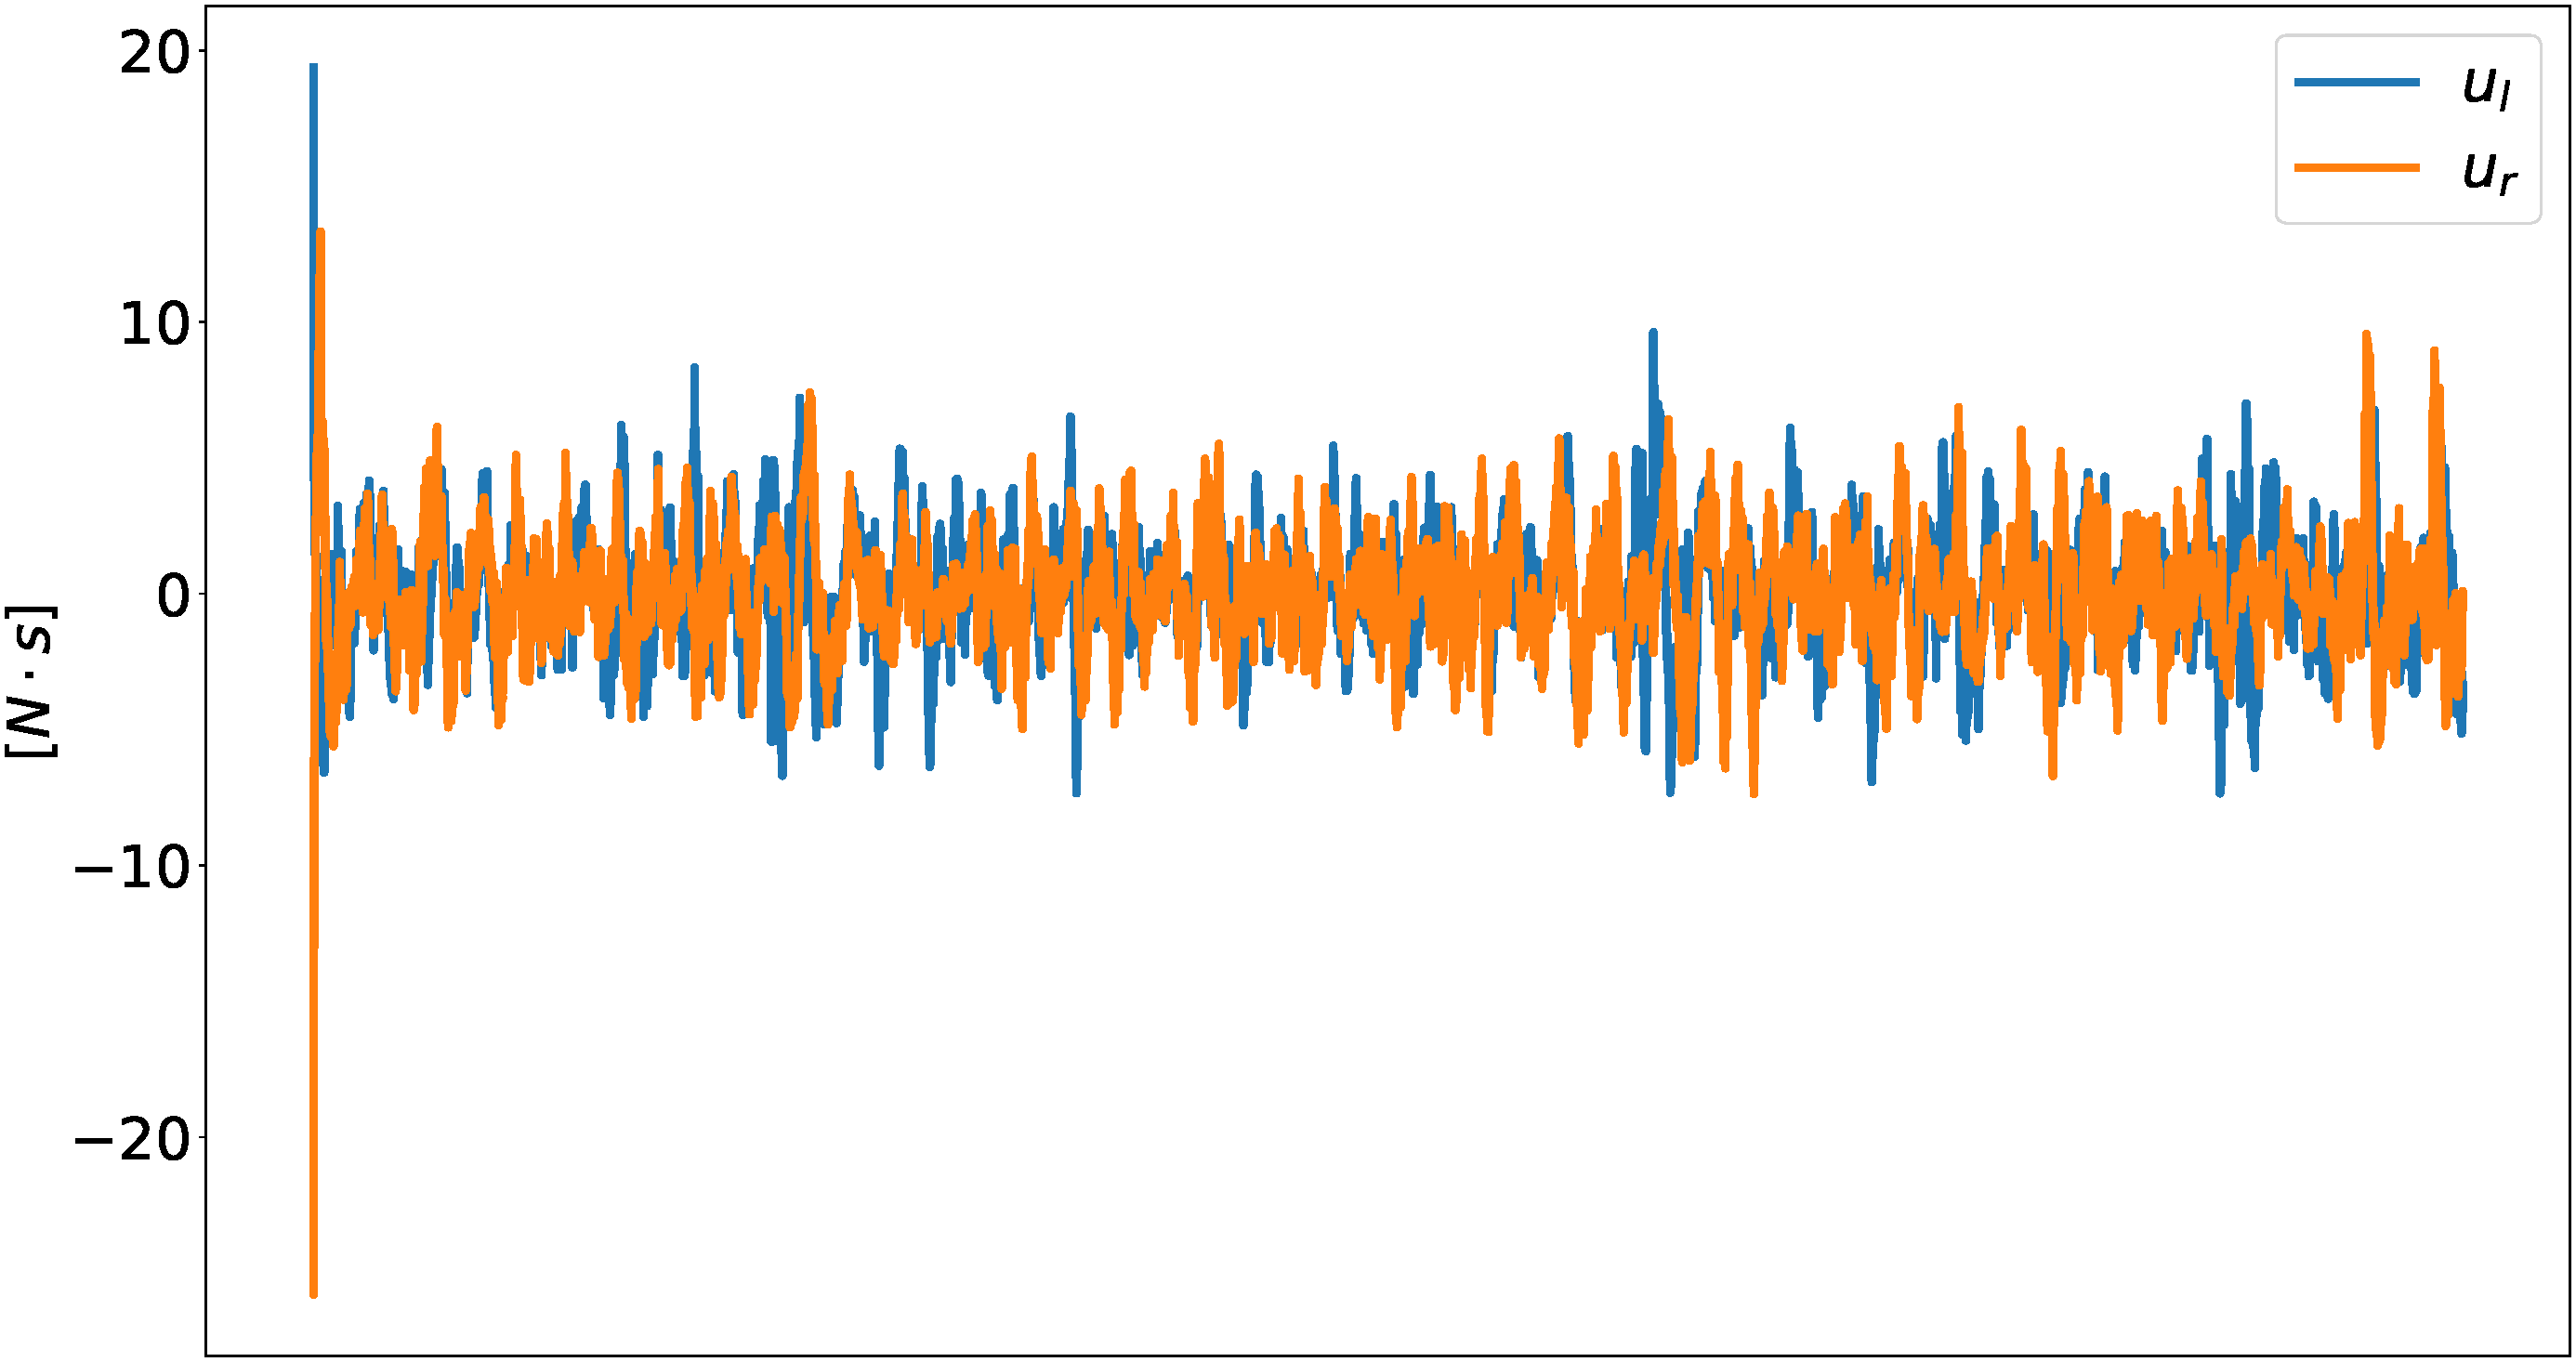
\includegraphics[width=0.49\linewidth]{Figures/Real time one stage OCP on rough terrain/Robustness tests/forces_rate_curve.pdf}}
  \end{subfigmatrix}
  \caption{Robustness test results of solver \ti{Low rate of change}, where $a=1.0,\,b=1.0,\,c=0.4$.}
  \label{fig:robustnessResultsSolver3}
\end{figure}